\documentclass[10pt,a4paper]{article}
\usepackage[a4paper,margin=16mm]{geometry}
\usepackage[T1]{fontenc}
\usepackage{lmodern}
\usepackage{amsmath,amssymb}
\usepackage{graphicx}
\usepackage{booktabs}
\usepackage{longtable}
\usepackage{array}
\usepackage{xcolor}
\usepackage{caption}
\usepackage{subcaption}
\usepackage{tikz}
\usetikzlibrary{arrows.meta,positioning,fit,calc,trees,shapes.misc}
\usepackage[hidelinks]{hyperref}
\usepackage{enumitem}
\usepackage{listings}
\setlist{nosep,leftmargin=1.2em}
\captionsetup{font=small,labelfont=bf}
\setlength{\parskip}{2pt}
\setlength{\emergencystretch}{3em}
\setcounter{tocdepth}{1}

\newcommand{\vect}[1]{\mathbf{#1}}
\newcommand{\code}[1]{\texttt{#1}}
\newcommand{\cli}[1]{\texttt{-{}-#1}}

% ---- status words used by the audit appendix -------------------------------------------------------------
\definecolor{okc}{RGB}{20,120,60}
\definecolor{partc}{RGB}{190,110,0}
\definecolor{nmc}{RGB}{170,40,40}
\newcommand{\sDone}{\textcolor{okc}{\textbf{done}}}
\newcommand{\sPart}{\textcolor{partc}{\textbf{partial}}}
\newcommand{\sNM}{\textcolor{nmc}{\textbf{not measured}}}

% ---- figures: a fallback box is printed while a captured image does not exist yet ---------------------
\newcommand{\pendingbox}[2]{%
  \fbox{\parbox[c][0.5625\dimexpr#2\relax][c]{\dimexpr#2-2\fboxsep-2\fboxrule\relax}{\centering\footnotesize\ttfamily
  figure pending:\\ \detokenize{#1}}}}
\newcommand{\pic}[2]{\IfFileExists{img/#1.jpg}{\includegraphics[width=#2]{img/#1.jpg}}{\IfFileExists{img/#1.png}{\includegraphics[width=#2]{img/#1.png}}{\IfFileExists{#1.png}{\includegraphics[width=#2]{#1.png}}{\pendingbox{#1}{#2}}}}}
\newcommand{\picdia}[2]{\pic{diagrams/#1}{#2}}      % matplotlib diagrams from program data (report/diagrams)
\newcommand{\piclab}[2]{\pic{figures_lab/#1}{#2}}   % in-program renders of single techniques (report/figures_lab)
\newcommand{\picfour}[2]{\IfFileExists{figures_v5/#1.png}{\pic{figures_v5/#1}{#2}}{\pic{figures_v4/#1}{#2}}}   % v4 shot names: the current v5 capture of the same shot
\newcommand{\picthree}[2]{\pic{figures_v3/#1}{#2}}  % v3 set
\newcommand{\pictwo}[2]{\pic{figures/#1}{#2}}       % v2 set
\newcommand{\picfive}[2]{\pic{figures_v5/#1}{#2}}  % v5 set (night-watch game)
\newcommand{\picsix}[2]{\pic{figures_v6/#1}{#2}}   % v6 set (day cycle, soldiers, real CV; RTX 4070 captures)


\definecolor{lstbg}{gray}{0.96}
\lstdefinelanguage{GLSL}{morekeywords={uniform,in,out,flat,vec2,vec3,vec4,mat3,mat4,float,int,bool,void,return,if,else,for,break,continue,const,layout,struct,sampler2D,sampler2DShadow,location,discard,smooth},
  morekeywords=[2]{normalize,dot,cross,reflect,mix,clamp,pow,max,min,abs,sqrt,smoothstep,step,texture,fract,floor,length,sin,cos,exp,any,lessThan,greaterThan,transpose,inverse},sensitive=true,morecomment=[l]{//},morestring=[b]"}
\lstset{basicstyle=\ttfamily\fontsize{6.8}{8}\selectfont,backgroundcolor=\color{lstbg},keywordstyle=\color{blue!60!black}\bfseries,keywordstyle=[2]\color{purple!70!black},
  commentstyle=\color{green!40!black}\itshape,numbers=left,numberstyle=\tiny\color{gray},numbersep=4pt,frame=single,rulecolor=\color{black!25},
  breaklines=true,breakatwhitespace=false,columns=fullflexible,keepspaces=true,showstringspaces=false,captionpos=b,
  aboveskip=4pt,belowskip=2pt,xleftmargin=10pt,framexleftmargin=8pt,tabsize=2,
  literate={→}{$\rightarrow$}1 {×}{$\times$}1 {·}{.}1 {²}{$^2$}1 {≈}{$\approx$}1 {≤}{$\le$}1 {≥}{$\ge$}1 {°}{$^\circ$}1 {—}{--}1 {–}{-}1 {µ}{u}1 {é}{e}1 {ü}{u}1 {α}{a}1 {β}{b}1 {ω}{w}1 {π}{pi}1 {σ}{s}1 {λ}{l}1 {Δ}{D}1 {⁻}{-}1 {¹}{1}1 {χ}{x}1,
  morekeywords={nullptr,constexpr,uint8_t,size_t,uint32_t,auto,std}}
\renewcommand{\lstlistingname}{Listing}
\captionsetup[lstlisting]{font=small,labelfont=bf}
% generated by report/listings.py -- do not edit
\newcommand{\lstCube}{\lstinputlisting[language=C++,firstline=24,lastline=44,caption={Cube generator: 24 vertices, 6 faces \textnormal{(\texttt{src/primitives/Cube.cpp}, lines 24--44)}},label={lst:Cube}]{../src/primitives/Cube.cpp}}
\newcommand{\lstSphere}{\lstinputlisting[language=C++,firstline=7,lastline=63,caption={Sphere generator (northern hemisphere, then reflection) \textnormal{(\texttt{src/primitives/Sphere.cpp}, lines 7--63)}},label={lst:Sphere}]{../src/primitives/Sphere.cpp}}
\newcommand{\lstCylinder}{\lstinputlisting[language=C++,firstline=26,lastline=54,caption={Cylinder / cone / frustum generator \textnormal{(\texttt{src/primitives/Cylinder.cpp}, lines 26--54)}},label={lst:Cylinder}]{../src/primitives/Cylinder.cpp}}
\newcommand{\lstPerspective}{\lstinputlisting[language=C++,firstline=84,lastline=94,caption={Perspective projection matrix \textnormal{(\texttt{src/math/Math3D.cpp}, lines 84--94)}},label={lst:Perspective}]{../src/math/Math3D.cpp}}
\newcommand{\lstLookAt}{\lstinputlisting[language=C++,firstline=107,lastline=116,caption={View matrix lookAt \textnormal{(\texttt{src/math/Math3D.cpp}, lines 107--116)}},label={lst:LookAt}]{../src/math/Math3D.cpp}}
\newcommand{\lstPart}{\lstinputlisting[language=C++,firstline=38,lastline=52,caption={Builder::part: one table row becomes one node \textnormal{(\texttt{src/objects/Builder.cpp}, lines 38--52)}},label={lst:Part}]{../src/objects/Builder.cpp}}
\newcommand{\lstTransform}{\lstinputlisting[language=C++,firstline=14,lastline=14,caption={Local matrix M = T R S \textnormal{(\texttt{src/scene/Transform.h}, lines 14--14)}},label={lst:Transform}]{../src/scene/Transform.h}}
\newcommand{\lstUpdateNode}{\lstinputlisting[language=C++,firstline=44,lastline=49,caption={World matrix = parent world times local (and the explode view) \textnormal{(\texttt{src/scene/Scene.cpp}, lines 44--49)}},label={lst:UpdateNode}]{../src/scene/Scene.cpp}}
\newcommand{\lstBrdf}{\lstinputlisting[language=GLSL,firstline=159,lastline=180,caption={Blinn-Phong and Cook-Torrance (GGX) in one function \textnormal{(\texttt{src/rendering/ShaderSources.cpp}, lines 159--180)}},label={lst:Brdf}]{../src/rendering/ShaderSources.cpp}}
\newcommand{\lstFlatGeom}{\lstinputlisting[language=GLSL,firstline=750,lastline=768,caption={Flat shading: one normal per triangle in a geometry shader \textnormal{(\texttt{src/rendering/ShaderSources.cpp}, lines 750--768)}},label={lst:FlatGeom}]{../src/rendering/ShaderSources.cpp}}
\newcommand{\lstGouraudVert}{\lstinputlisting[language=GLSL,firstline=781,lastline=798,caption={Gouraud shading: lighting per vertex \textnormal{(\texttt{src/rendering/ShaderSources.cpp}, lines 781--798)}},label={lst:GouraudVert}]{../src/rendering/ShaderSources.cpp}}
\newcommand{\lstPractical}{\lstinputlisting[language=GLSL,firstline=136,lastline=145,caption={Practical light attenuation (windowed inverse square) \textnormal{(\texttt{src/rendering/ShaderSources.cpp}, lines 136--145)}},label={lst:Practical}]{../src/rendering/ShaderSources.cpp}}
\newcommand{\lstIndoor}{\lstinputlisting[language=GLSL,firstline=125,lastline=134,caption={Indoor mask \textnormal{(\texttt{src/rendering/ShaderSources.cpp}, lines 125--134)}},label={lst:Indoor}]{../src/rendering/ShaderSources.cpp}}
\newcommand{\lstMoonShadow}{\lstinputlisting[language=GLSL,firstline=332,lastline=341,caption={Cascaded moon shadow lookup with PCF \textnormal{(\texttt{src/rendering/ShaderSources.cpp}, lines 332--341)}},label={lst:MoonShadow}]{../src/rendering/ShaderSources.cpp}}
\newcommand{\lstBump}{\lstinputlisting[language=GLSL,firstline=496,lastline=511,caption={Procedural bump: height gradient tilts the normal \textnormal{(\texttt{src/rendering/ShaderSources.cpp}, lines 496--511)}},label={lst:Bump}]{../src/rendering/ShaderSources.cpp}}
\newcommand{\lstAces}{\lstinputlisting[language=GLSL,firstline=389,lastline=396,caption={Fitted ACES tone-mapping curve \textnormal{(\texttt{src/rendering/ShadersPostFx.cpp}, lines 389--396)}},label={lst:Aces}]{../src/rendering/ShadersPostFx.cpp}}
\newcommand{\lstSsr}{\lstinputlisting[language=GLSL,firstline=44,lastline=83,caption={Screen-space reflection: ray march, bisection, Fresnel, edge fade \textnormal{(\texttt{src/rendering/ShadersPostFx.cpp}, lines 44--83)}},label={lst:Ssr}]{../src/rendering/ShadersPostFx.cpp}}
\newcommand{\lstFlood}{\lstinputlisting[language=C++,firstline=132,lastline=169,caption={MicroMouse flood fill (breadth-first search) from the hiding cells \textnormal{(\texttt{src/ai/HideController.cpp}, lines 132--169)}},label={lst:Flood}]{../src/ai/HideController.cpp}}
\newcommand{\lstDijkstra}{\lstinputlisting[language=C++,firstline=216,lastline=251,caption={Weighted flood fill (Dijkstra) from the objective: distance + exposure + noise \textnormal{(\texttt{src/ai/HideController.cpp}, lines 216--251)}},label={lst:Dijkstra}]{../src/ai/HideController.cpp}}
\newcommand{\lstDescend}{\lstinputlisting[language=C++,firstline=171,lastline=198,caption={Steepest descent through the distance field \textnormal{(\texttt{src/ai/HideController.cpp}, lines 171--198)}},label={lst:Descend}]{../src/ai/HideController.cpp}}
\newcommand{\lstChaikin}{\lstinputlisting[language=C++,firstline=29,lastline=42,caption={Chaikin corner cutting \textnormal{(\texttt{src/ai/HideController.cpp}, lines 29--42)}},label={lst:Chaikin}]{../src/ai/HideController.cpp}}
\newcommand{\lstFollowLine}{\lstinputlisting[language=C++,firstline=384,lastline=456,caption={Line follower: IR sensors, PD steering, differential drive \textnormal{(\texttt{src/ai/HideController.cpp}, lines 384--456)}},label={lst:FollowLine}]{../src/ai/HideController.cpp}}
\newcommand{\lstOtsu}{\lstinputlisting[language=C++,firstline=9,lastline=32,caption={Otsu's threshold \textnormal{(\texttt{src/vision/CvPipeline.cpp}, lines 9--32)}},label={lst:Otsu}]{../src/vision/CvPipeline.cpp}}
\newcommand{\lstDespeckle}{\lstinputlisting[language=C++,firstline=34,lastline=52,caption={Despeckle \textnormal{(\texttt{src/vision/CvPipeline.cpp}, lines 34--52)}},label={lst:Despeckle}]{../src/vision/CvPipeline.cpp}}
\newcommand{\lstLabel}{\lstinputlisting[language=C++,firstline=66,lastline=108,caption={Two-pass union-find labelling \textnormal{(\texttt{src/vision/CvPipeline.cpp}, lines 66--108)}},label={lst:Label}]{../src/vision/CvPipeline.cpp}}
\newcommand{\lstDetect}{\lstinputlisting[language=C++,firstline=180,lastline=189,caption={The image stage: threshold, despeckle, label, moments, filter \textnormal{(\texttt{src/vision/CvPipeline.cpp}, lines 180--189)}},label={lst:Detect}]{../src/vision/CvPipeline.cpp}}
\newcommand{\lstRayGround}{\lstinputlisting[language=C++,firstline=53,lastline=67,caption={Pixel ray to ground point \textnormal{(\texttt{src/ai/DroneController.cpp}, lines 53--67)}},label={lst:RayGround}]{../src/ai/DroneController.cpp}}
\newcommand{\lstPredict}{\lstinputlisting[language=C++,firstline=19,lastline=44,caption={Kalman prediction with white-noise-acceleration Q \textnormal{(\texttt{src/vision/MultiTracker.cpp}, lines 19--44)}},label={lst:Predict}]{../src/vision/MultiTracker.cpp}}
\newcommand{\lstKalman}{\lstinputlisting[language=C++,firstline=55,lastline=74,caption={Kalman measurement update \textnormal{(\texttt{src/vision/MultiTracker.cpp}, lines 55--74)}},label={lst:Kalman}]{../src/vision/MultiTracker.cpp}}
\newcommand{\lstMahal}{\lstinputlisting[language=C++,firstline=46,lastline=53,caption={Mahalanobis distance for gating \textnormal{(\texttt{src/vision/MultiTracker.cpp}, lines 46--53)}},label={lst:Mahal}]{../src/vision/MultiTracker.cpp}}
\newcommand{\lstHungarian}{\lstinputlisting[language=C++,firstline=76,lastline=131,caption={Hungarian algorithm \textnormal{(\texttt{src/vision/MultiTracker.cpp}, lines 76--131)}},label={lst:Hungarian}]{../src/vision/MultiTracker.cpp}}
\newcommand{\lstTriangulate}{\lstinputlisting[language=C++,firstline=133,lastline=146,caption={Two-view triangulation \textnormal{(\texttt{src/vision/MultiTracker.cpp}, lines 133--146)}},label={lst:Triangulate}]{../src/vision/MultiTracker.cpp}}
\newcommand{\lstFlightTime}{\lstinputlisting[language=C++,firstline=43,lastline=50,caption={Round flight-time model for time-on-target \textnormal{(\texttt{src/ai/Squad.cpp}, lines 43--50)}},label={lst:FlightTime}]{../src/ai/Squad.cpp}}
\newcommand{\lstSunDir}{\lstinputlisting[language=C++,firstline=112,lastline=119,caption={Solar position: hour angle, latitude and declination to the unit vector towards the sun \textnormal{(\texttt{src/scene/DayCycle.cpp}, lines 112--119)}},label={lst:SunDir}]{../src/scene/DayCycle.cpp}}
\newcommand{\lstAirMass}{\lstinputlisting[language=C++,firstline=133,lastline=141,caption={Kasten--Young air mass and the per-channel sun transmittance \textnormal{(\texttt{src/scene/DayCycle.cpp}, lines 133--141)}},label={lst:AirMass}]{../src/scene/DayCycle.cpp}}
\newcommand{\lstApparentHeat}{\lstinputlisting[language=C++,firstline=352,lastline=370,caption={Solar loading of passive surfaces, cloud density and cloud shadow (CPU mirror of the shader) \textnormal{(\texttt{src/scene/DayCycle.cpp}, lines 352--370)}},label={lst:ApparentHeat}]{../src/scene/DayCycle.cpp}}
\newcommand{\lstSplineSeg}{\lstinputlisting[language=C++,firstline=71,lastline=88,caption={Centripetal Catmull--Rom segment as a cubic Hermite curve (position, first and second derivative) \textnormal{(\texttt{src/math/Spline.cpp}, lines 71--88)}},label={lst:SplineSeg}]{../src/math/Spline.cpp}}
\newcommand{\lstArcLen}{\lstinputlisting[language=C++,firstline=113,lastline=128,caption={Arc-length parameterisation: binary search in the cumulative chord table \textnormal{(\texttt{src/math/Spline.cpp}, lines 113--128)}},label={lst:ArcLen}]{../src/math/Spline.cpp}}
\newcommand{\lstLegIK}{\lstinputlisting[language=C++,firstline=73,lastline=87,caption={Two-link leg IK (law of cosines) and its forward kinematics \textnormal{(\texttt{src/scene/Gait.cpp}, lines 73--87)}},label={lst:LegIK}]{../src/scene/Gait.cpp}}
\newcommand{\lstFootPath}{\lstinputlisting[language=C++,firstline=59,lastline=71,caption={Ankle trajectory: world-locked stance, cycloid swing with a sine lift \textnormal{(\texttt{src/scene/Gait.cpp}, lines 59--71)}},label={lst:FootPath}]{../src/scene/Gait.cpp}}
\newcommand{\lstArmIK}{\lstinputlisting[language=C++,firstline=268,lastline=294,caption={Two-bone arm IK with a pole vector (rifle hold), result as Euler angles of the shoulder \textnormal{(\texttt{src/scene/Gait.cpp}, lines 268--294)}},label={lst:ArmIK}]{../src/scene/Gait.cpp}}
\newcommand{\lstAStar}{\lstinputlisting[language=C++,firstline=235,lastline=301,caption={Site planner: 8-connected A* with the octile heuristic and no corner cutting \textnormal{(\texttt{src/scene/Garrison.cpp}, lines 235--301)}},label={lst:AStar}]{../src/scene/Garrison.cpp}}
\newcommand{\lstStringPull}{\lstinputlisting[language=C++,firstline=303,lastline=330,caption={Greedy string pulling with sampled clearance checks \textnormal{(\texttt{src/scene/Garrison.cpp}, lines 303--330)}},label={lst:StringPull}]{../src/scene/Garrison.cpp}}
\newcommand{\lstSpeedLaw}{\lstinputlisting[language=C++,firstline=889,lastline=930,caption={Route following: curvature speed law with look-ahead braking \textnormal{(\texttt{src/scene/Garrison.cpp}, lines 889--930)}},label={lst:SpeedLaw}]{../src/scene/Garrison.cpp}}
\newcommand{\lstRandomRoute}{\lstinputlisting[language=C++,firstline=89,lastline=139,caption={Random route of an intruder: ring spawn, via sector, personality, objective switch \textnormal{(\texttt{src/scene/Mission.cpp}, lines 89--139)}},label={lst:RandomRoute}]{../src/scene/Mission.cpp}}
\newcommand{\lstDeriveSeed}{\lstinputlisting[language=C++,firstline=205,lastline=212,caption={Independent random streams from one run seed (splitmix32 finaliser) \textnormal{(\texttt{src/scene/Scene.cpp}, lines 205--212)}},label={lst:DeriveSeed}]{../src/scene/Scene.cpp}}
\newcommand{\lstSensorApply}{\lstinputlisting[language=C++,firstline=83,lastline=135,caption={SensorModel::apply: PSF, fixed pattern, NETD, quantisation, stuck pixels and bad-pixel replacement \textnormal{(\texttt{src/vision/SensorModel.cpp}, lines 83--135)}},label={lst:SensorApply}]{../src/vision/SensorModel.cpp}}
\newcommand{\lstClassify}{\lstinputlisting[language=C++,firstline=191,lastline=199,caption={Blob classes: target, hot clutter, person, clutter \textnormal{(\texttt{src/vision/CvPipeline.cpp}, lines 191--199)}},label={lst:Classify}]{../src/vision/CvPipeline.cpp}}


% ---- "where we are in the pipeline" strip: \pipestrip{k} highlights stage k (1..10) ----------------------------------------
\newcommand{\psnode}[3]{\ifnum#1=#2 \node[draw,rounded corners=1pt,fill=orange!55,minimum width=1.5cm,minimum height=0.75cm,align=center,line width=0.8pt] at (1.62*#1,0) {#3};\else \node[draw,rounded corners=1pt,fill=black!5,minimum width=1.5cm,minimum height=0.75cm,align=center,text=black!60] at (1.62*#1,0) {#3};\fi}
\newcommand{\pipestrip}[1]{\begin{center}\begin{tikzpicture}[font=\fontsize{5.6}{6.4}\selectfont]
 \psnode{1}{#1}{vertex data}
 \psnode{2}{#1}{model\\matrix $TRS$}
 \psnode{3}{#1}{view +\\projection}
 \psnode{4}{#1}{clip/NDC\\viewport}
 \psnode{5}{#1}{raster\\interpolation}
 \psnode{6}{#1}{fragment\\shading}
 \psnode{7}{#1}{depth +\\shadows}
 \psnode{8}{#1}{HDR post\\SSR/TAA}
 \psnode{9}{#1}{heat render\\+ vision}
 \psnode{10}{#1}{tracking +\\decisions}
 \foreach \x in {1,...,9} \draw[-{Latex[length=1mm]},black!50] ({1.62*\x+0.75},0) -- ({1.62*\x+0.87},0);
\end{tikzpicture}\end{center}\vspace{-3mm}}
\newcommand{\picsheet}[2]{\pic{sheets/#1}{#2}}   % Excel workbook screenshots (report/sheets)
% generated by report/sheet_figs.py from sheets/captions.json -- do not edit
\providecommand{\sheetcaption}[1]{\ifcsname sheetcap@#1\endcsname\csname sheetcap@#1\endcsname\else\texttt{#1}\fi}
\providecommand{\sheetfig}[2][\linewidth]{\begin{figure}[htbp]\centering\picsheet{#2}{#1}\caption{\sheetcaption{#2}}\label{fig:sheet:#2}\end{figure}}
\expandafter\def\csname sheetcap@s00_cover_kpis\endcsname{Workbook sheet \emph{0 Cover \& Index}, cells \texttt{A1:I19}: Cover sheet: author block and the two KPI tile rows, every number computed by an Excel formula or exported from the program.}
\expandafter\def\csname sheetcap@s02_cube_indices\endcsname{Workbook sheet \emph{2 Primitive Vertex Data}, cells \texttt{J4:O17}: Cube index buffer: 12 triangles = 36 indices; column O is an Excel formula testing the winding with n0 . ((p1-p0) x (p2-p0)) (green = CCW = front face).}
\expandafter\def\csname sheetcap@s02_sphere_cylinder\endcsname{Workbook sheet \emph{2 Primitive Vertex Data}, cells \texttt{A42:Q55}: Sphere and cylinder vertex data (first 12 vertices each); the check columns |p| = 0.5 and sqrt(x\textasciicircum{}2+y\textasciicircum{}2) = 0.5 confirm the parametrisation.}
\expandafter\def\csname sheetcap@s03_aagun\endcsname{Workbook sheet \emph{3 Object Construction}, cells \texttt{A4:Q3454}: Construction rows of the aa gatling gun (17 rows of 83 shown; row labels are the real sheet rows). Every part is one primitive with S, R (degrees) and T relative to its parent; shading model in the last column. AA Gatling gun: pedestal, yaw / pitch mount, rotating barrel cluster.}
\expandafter\def\csname sheetcap@s03_bunker\endcsname{Workbook sheet \emph{3 Object Construction}, cells \texttt{A4:Q1331}: Construction rows of the command bunker (21 rows of 417 shown; row labels are the real sheet rows). Every part is one primitive with S, R (degrees) and T relative to its parent; shading model in the last column. Command bunker (underground, 400 parts): walls, ramp, blast doors and rooms as cubes and cylinders.}
\expandafter\def\csname sheetcap@s03_flag\endcsname{Workbook sheet \emph{3 Object Construction}, cells \texttt{A4:Q5242}: Construction rows of the flag (16 rows of 61 shown; row labels are the real sheet rows). Every part is one primitive with S, R (degrees) and T relative to its parent; shading model in the last column. Flag: pole and a chain of cloth strips each yawed by a travelling wave.}
\expandafter\def\csname sheetcap@s03_gate\endcsname{Workbook sheet \emph{3 Object Construction}, cells \texttt{A4:Q5159}: Construction rows of the boom barrier (12 rows of 22 shown; row labels are the real sheet rows). Every part is one primitive with S, R (degrees) and T relative to its parent; shading model in the last column. Gate boom barrier: post, counterweight and pivoting boom with stripes.}
\expandafter\def\csname sheetcap@s03_helicopter\endcsname{Workbook sheet \emph{3 Object Construction}, cells \texttt{A4:Q3371}: Construction rows of the scout helicopter (19 rows of 110 shown; row labels are the real sheet rows). Every part is one primitive with S, R (degrees) and T relative to its parent; shading model in the last column. Scout helicopter: fuselage, main rotor and tail rotor groups.}
\expandafter\def\csname sheetcap@s03_mlrs\endcsname{Workbook sheet \emph{3 Object Construction}, cells \texttt{A4:Q3845}: Construction rows of the mlrs rocket truck (21 rows of 158 shown; row labels are the real sheet rows). Every part is one primitive with S, R (degrees) and T relative to its parent; shading model in the last column. MLRS rocket truck: cab, elevating pod frame and rocket tubes.}
\expandafter\def\csname sheetcap@s03_primitive_mix\endcsname{Workbook sheet \emph{3 Object Construction}, cells \texttt{AA3:AI25}: Primitive mix per final object: how many cylinders, spheres, cones, cubes and frusta (and how many group nodes) build each object; Excel COUNTIFS over the 4 549-row construction table.}
\expandafter\def\csname sheetcap@s03_radar\endcsname{Workbook sheet \emph{3 Object Construction}, cells \texttt{A4:Q3566}: Construction rows of the air-defence radar (16 rows of 112 shown; row labels are the real sheet rows). Every part is one primitive with S, R (degrees) and T relative to its parent; shading model in the last column. Air-defence radar: tower and rotating antenna of tiles.}
\expandafter\def\csname sheetcap@s03_rover\endcsname{Workbook sheet \emph{3 Object Construction}, cells \texttt{A4:Q2837}: Construction rows of the target rover (13 rows of 28 shown; row labels are the real sheet rows). Every part is one primitive with S, R (degrees) and T relative to its parent; shading model in the last column. Target rover: chassis, wheels, thermal engine block (heat column drives the thermal camera).}
\expandafter\def\csname sheetcap@s03_sam\endcsname{Workbook sheet \emph{3 Object Construction}, cells \texttt{A4:Q3687}: Construction rows of the sam launcher (20 rows of 121 shown; row labels are the real sheet rows). Every part is one primitive with S, R (degrees) and T relative to its parent; shading model in the last column. SAM launcher: chassis, elevating launcher frame and missile tubes.}
\expandafter\def\csname sheetcap@s03_tank_material\endcsname{Workbook sheet \emph{3 Object Construction}, cells \texttt{A4:X5000}: Tank rows, material and thermal columns: shading, procedural surface, roughness, metalness, heat (thermal-camera value), emissive, animation text.}
\expandafter\def\csname sheetcap@s03_uav\endcsname{Workbook sheet \emph{3 Object Construction}, cells \texttt{A4:Q1427}: Construction rows of the autonomous uav (22 rows of 96 shown; row labels are the real sheet rows). Every part is one primitive with S, R (degrees) and T relative to its parent; shading model in the last column. Autonomous UAV: fuselage, four motor mounts with rotor groups, gimbal yaw / pitch chain, searchlight.}
\expandafter\def\csname sheetcap@s04_inputs_blocks\endcsname{Workbook sheet \emph{4 Transform Matrices}, cells \texttt{AY4:BL22}: Worked example inputs (S, R in degrees, T looked up by component ID with INDEX / MATCH) and the translation, yaw, pitch blocks, plus Ry x Rx.}
\expandafter\def\csname sheetcap@s04_rows_error\endcsname{Workbook sheet \emph{4 Transform Matrices}, cells \texttt{A3:AW40}: Per-component rows of sheet 4 for the UAV gimbal chain: S, R, T inputs, the 3x3 rotation entries and the max-error column (Excel M versus the code's matrix).}
\expandafter\def\csname sheetcap@s04_rows_m\endcsname{Workbook sheet \emph{4 Transform Matrices}, cells \texttt{A3:AW40}: The 12 M entries computed by Excel for the gimbal chain next to the code's matrix, and the max |difference| column.}
\expandafter\def\csname sheetcap@s05_tank_chain\endcsname{Workbook sheet \emph{5 Hierarchy}, cells \texttt{A3:AI1850}: Hierarchy sheet, tank chain: tank root \textgreater{} hull \textgreater{} turret yaw \textgreater{} gun pitch \textgreater{} mantlet / barrel recoil. Depth increases by one per joint.}
\expandafter\def\csname sheetcap@s05_world_matrix\endcsname{Workbook sheet \emph{5 Hierarchy}, cells \texttt{A4:AG1850}: World matrices of the UAV gimbal chain computed by Excel: W = W\_parent x M (each W cell is a sum of products referencing the parent's row and sheet 4), next to the code's values.}
\expandafter\def\csname sheetcap@s06_charts\endcsname{Workbook sheet \emph{6 Geometry Statistics}, cells \texttt{A13:S34}: Memory charts: bytes per mesh indexed versus non-indexed (drawn from the sheet's chart definitions).}
\expandafter\def\csname sheetcap@s06_geometry_stats\endcsname{Workbook sheet \emph{6 Geometry Statistics}, cells \texttt{A4:P11}: Memory of every GPU mesh: indexed versus non-indexed, per-mesh saving and vertex reuse, and the formula vs exporter check.}
\expandafter\def\csname sheetcap@s07_attenuation\endcsname{Workbook sheet \emph{7 Lighting}, cells \texttt{A14:K32}: Distance attenuation 1/(1 + k1 d + k2 d\textasciicircum{}2) for the beacon and the searchlight, and the spotlight cone factor versus angle; all Excel formulas.}
\expandafter\def\csname sheetcap@s07_charts\endcsname{Workbook sheet \emph{7 Lighting}, cells \texttt{M14:Z50}: Attenuation and cone curves drawn from the sheet's scatter charts.}
\expandafter\def\csname sheetcap@s08_comparison\endcsname{Workbook sheet \emph{8 Shading}, cells \texttt{A12:J31}: Same bunker, same camera: flat, Gouraud and Phong override side by side (renders from the program).}
\expandafter\def\csname sheetcap@s08_shading\endcsname{Workbook sheet \emph{8 Shading}, cells \texttt{A4:H13}: Shading models used in the scene: parts using each (COUNTIF), which normal is used, where lighting is evaluated, cost and visual effect.}
\expandafter\def\csname sheetcap@s09_features\endcsname{Workbook sheet \emph{9 Render Pipeline}, cells \texttt{A5:H17}: Per-feature frame cost: configuration, frame time, baseline, feature cost and share (differences computed by Excel).}
\expandafter\def\csname sheetcap@s09_pipeline_passes\endcsname{Workbook sheet \emph{9 Render Pipeline}, cells \texttt{A20:D30}: GPU pass list of one frame (measured): time per pass, share of the total and cumulative time, Excel formulas.}
\expandafter\def\csname sheetcap@s10_testing\endcsname{Workbook sheet \emph{10 Testing}, cells \texttt{A1:G30}: Test sheet: KPI row (tests, passed, failed, pass rate - Excel formulas over the status column) and the first 25 tests with expected and observed results.}
\expandafter\def\csname sheetcap@s14_aagun\endcsname{Workbook sheet \emph{14 Controllable Objects}, cells \texttt{A173:L650}: Controllable AA-1 GATLING: the moving parts and the animation rule of each articulated node, as exported from the code.}
\expandafter\def\csname sheetcap@s14_derived\endcsname{Workbook sheet \emph{14 Controllable Objects}, cells \texttt{A156:D169}: Derived figures computed by Excel from the specification table (e.g. turret 360 degrees = 360 / slew rate).}
\expandafter\def\csname sheetcap@s14_doors\endcsname{Workbook sheet \emph{14 Controllable Objects}, cells \texttt{A173:L650}: Controllable BLAST DOORS: the moving parts and the animation rule of each articulated node, as exported from the code.}
\expandafter\def\csname sheetcap@s14_gate\endcsname{Workbook sheet \emph{14 Controllable Objects}, cells \texttt{A173:L650}: Controllable GATE BARRIER: the moving parts and the animation rule of each articulated node, as exported from the code.}
\expandafter\def\csname sheetcap@s14_helicopter\endcsname{Workbook sheet \emph{14 Controllable Objects}, cells \texttt{A173:L650}: Controllable MH-6 HELICOPTER: the moving parts and the animation rule of each articulated node, as exported from the code.}
\expandafter\def\csname sheetcap@s14_mlrs\endcsname{Workbook sheet \emph{14 Controllable Objects}, cells \texttt{A173:L650}: Controllable MLRS-1 ROCKET TRUCK: the moving parts and the animation rule of each articulated node, as exported from the code.}
\expandafter\def\csname sheetcap@s14_radar\endcsname{Workbook sheet \emph{14 Controllable Objects}, cells \texttt{A173:L650}: Controllable AIR-DEFENCE RADAR: the moving parts and the animation rule of each articulated node, as exported from the code.}
\expandafter\def\csname sheetcap@s14_sam\endcsname{Workbook sheet \emph{14 Controllable Objects}, cells \texttt{A173:L650}: Controllable SAM-1 LAUNCHER: the moving parts and the animation rule of each articulated node, as exported from the code.}
\expandafter\def\csname sheetcap@s14_specs_tank\endcsname{Workbook sheet \emph{14 Controllable Objects}, cells \texttt{A24:F60}: Specification rows of the tank read from the code constants, with the Excel-derived figures in sheet 14 below them.}
\expandafter\def\csname sheetcap@s14_tank\endcsname{Workbook sheet \emph{14 Controllable Objects}, cells \texttt{A173:L650}: Controllable MBT-1 TANK: the moving parts and the animation rule of each articulated node, as exported from the code.}
\expandafter\def\csname sheetcap@s14_uav\endcsname{Workbook sheet \emph{14 Controllable Objects}, cells \texttt{A173:L650}: Controllable UAV-1 DRONE: the moving parts and the animation rule of each articulated node, as exported from the code.}
\expandafter\def\csname sheetcap@s16_effects\endcsname{Workbook sheet \emph{16 Combat \& Effects}, cells \texttt{A43:G54}: Particle effects measured by running the real Combat code: particle count, peak, lifetime and dynamic light for each effect.}
\expandafter\def\csname sheetcap@s16_weapons\endcsname{Workbook sheet \emph{16 Combat \& Effects}, cells \texttt{A35:I40}: Weapons: speeds, blast power, damage radius (= power x kDamageRadiusPerPower), flight time, range, reload and guidance; formulas over the constants table.}
\expandafter\def\csname sheetcap@s18_params_footprint\endcsname{Workbook sheet \emph{18 Computer Vision}, cells \texttt{A40:E59}: Derived camera figures (pixels per degree, horizontal FOV, gate radius) and the ground footprint of one pixel versus UAV altitude, all Excel formulas.}
\expandafter\def\csname sheetcap@s18_tests\endcsname{Workbook sheet \emph{18 Computer Vision}, cells \texttt{A63:E73}: Vision tests T130-T137 with their PASS status looked up from the testing sheet (INDEX / MATCH).}
\expandafter\def\csname sheetcap@s19_armour\endcsname{Workbook sheet \emph{19 Squad \& Mission}, cells \texttt{A102:D117}: Armour and damage falloff: damage per round, rounds to kill with one or two UAVs and the reload of one UAV, Excel formulas.}
\expandafter\def\csname sheetcap@s19_combined\endcsname{Workbook sheet \emph{19 Squad \& Mission}, cells \texttt{A65:G71}: Combined strike: launch delay of the nearer UAV so both rounds arrive together (arrival spread = 0).}
\expandafter\def\csname sheetcap@s19_roles\endcsname{Workbook sheet \emph{19 Squad \& Mission}, cells \texttt{A4:C16}: Squad roles and strike phases.}
\expandafter\def\csname sheetcap@s19_waves\endcsname{Workbook sheet \emph{19 Squad \& Mission}, cells \texttt{A74:D100}: Mission constants: waves, base integrity and score parameters from the code.}
\expandafter\def\csname sheetcap@s20_hud_tests\endcsname{Workbook sheet \emph{20 Audio \& HUD}, cells \texttt{A56:E71}: Audio tests with PASS status looked up from sheet 10.}
\expandafter\def\csname sheetcap@s20_mixer\endcsname{Workbook sheet \emph{20 Audio \& HUD}, cells \texttt{A24:C35}: Mixer: sample rate, voices, panning, distance gain, air absorption, Doppler.}
\expandafter\def\csname sheetcap@s20_sounds\endcsname{Workbook sheet \emph{20 Audio \& HUD}, cells \texttt{A4:D21}: Synthesised sounds: trigger, technique and key parameters of all 15 sounds (no sample files).}
\expandafter\def\csname sheetcap@sheet_construction_tank\endcsname{Workbook sheet \emph{3 Object Construction}, cells \texttt{A4:Q3261}: Construction rows of the main battle tank (14 rows of 284 shown; row labels are the real sheet rows). Every part is one primitive with S, R (degrees) and T relative to its parent; shading model in the last column. Main battle tank: hull, tracks, turret yaw, gun pitch and recoil group.}
\expandafter\def\csname sheetcap@sheet_controllables\endcsname{Workbook sheet \emph{14 Controllable Objects}, cells \texttt{A3:L21}: All controllable objects: root, part counts per primitive, group nodes and animated nodes (Excel SUMIFS over the construction sheet).}
\expandafter\def\csname sheetcap@sheet_cv\endcsname{Workbook sheet \emph{18 Computer Vision}, cells \texttt{A4:E16}: Computer-vision pipeline: the 11 stages from the adaptive threshold to the Kalman track life cycle, with the code location of each.}
\expandafter\def\csname sheetcap@sheet_cvnoise\endcsname{Workbook sheet \emph{23 CV Noise \& Seeds}, cells \texttt{A1:H60}: CV Noise \& Seeds: sensor noise configuration, P\_d / false-alarm sweep against NETD, derived stream seeds and the v6 tests with the status looked up from the testing sheet.}
\expandafter\def\csname sheetcap@sheet_daycycle\endcsname{Workbook sheet \emph{21 Day Cycle \& Lighting}, cells \texttt{A1:W40}: Day Cycle \& Lighting: the exported 24 h grid (sun elevation, key intensity, ambient, fog, exposure, solar, beams, waves, cloud-shadow mean) with the Excel recomputation of the sun elevation from latitude, declination and hour, the difference and the OK check.}
\expandafter\def\csname sheetcap@sheet_hierarchy\endcsname{Workbook sheet \emph{5 Hierarchy}, cells \texttt{A3:AI1850}: Hierarchy sheet, UAV gimbal chain: UAV root \textgreater{} gimbal yaw \textgreater{} gimbal pitch \textgreater{} lamp / lens / camera; world position and the Excel-vs-code check, with the animation text of each joint.}
\expandafter\def\csname sheetcap@sheet_lighting\endcsname{Workbook sheet \emph{7 Lighting}, cells \texttt{A4:R8}: The three scene lights plus the ambient term: type, position, direction, colour, intensity, attenuation coefficients (k linear, k quadratic), spot cone angles, role.}
\expandafter\def\csname sheetcap@sheet_memory\endcsname{Workbook sheet \emph{2 Primitive Vertex Data}, cells \texttt{J20:Q39}: Technique 1 (separate triangles) versus Technique 2 (unique vertices + indices) for one face and for the whole cube; every figure is an Excel formula and the last row checks it against the exporter's byte count.}
\expandafter\def\csname sheetcap@sheet_mission\endcsname{Workbook sheet \emph{19 Squad \& Mission}, cells \texttt{A40:F62}: Time-on-target model of the rail rounds: ramp distance, flight time t(d) and its closed-form check against roundFlightTime(d); the last row confirms formula = code.}
\expandafter\def\csname sheetcap@sheet_mmult\endcsname{Workbook sheet \emph{4 Transform Matrices}, cells \texttt{BD11:BQ29}: Worked example for one component (CAMP-55): rotation blocks Ry, Rx, Rz, then R = Ry x Rx x Rz, T x R and finally M = T x R x S, every cell an Excel sum of products; the last block is |M - M\_code|.}
\expandafter\def\csname sheetcap@sheet_soldiers\endcsname{Workbook sheet \emph{22 Soldiers \& Routes}, cells \texttt{A1:Q40}: Soldiers \& Routes: roster with day / night duty, primitive counts per soldier (Excel totals), route lengths, joint tree and gait constants.}
\expandafter\def\csname sheetcap@sheet_vertex_cube\endcsname{Workbook sheet \emph{2 Primitive Vertex Data}, cells \texttt{A4:H29}: Cube vertex buffer: 24 unique vertices (4 per face) as interleaved x, y, z, nx, ny, nz; the face is derived from the normal by an Excel formula. (The lab primitives carry no texture coordinates.)}
\providecommand{\autocaption}[2]{\ifcsname figcap@#1@#2\endcsname\csname figcap@#1@#2\endcsname\else\texttt{#2}\fi}
\providecommand{\autofig}[3][\linewidth]{\begin{figure}[htbp]\centering\pic{#2/#3}{#1}\caption{\autocaption{#2}{#3}}\label{fig:#2:#3}\end{figure}}
\expandafter\def\csname figcap@diagrams@A1_cube_vertices\endcsname{The unit cube generator: 24 vertices (4 per face, each with the face normal) and 36 indices (2 counter-clockwise triangles per face, diagonal 0-2). Indexed storage needs 720 B instead of 864 B. {\footnotesize(Source: \texttt{src/primitives/Cube.cpp: createCube()})}}
\expandafter\def\csname figcap@diagrams@A2_sphere_rings\endcsname{The sphere generator: 614 vertices on 9 rings x 36 slices per hemisphere, 1224 triangles; the normal of every vertex equals its normalised position, the southern half is the mirrored northern half. {\footnotesize(Source: \texttt{src/primitives/Sphere.cpp: createSphere(36, 18)})}}
\expandafter\def\csname figcap@diagrams@A3_cylinder_cone\endcsname{Cylinder, cone and frustum come from one generator: two interleaved rings (bottom z = -0.5, top z = +0.5), side triangles, and a triangle fan per cap; a cone is simply top radius 0, the beam frustum has no caps. {\footnotesize(Source: \texttt{src/primitives/Cylinder.cpp: createCylinder(); Renderer.cpp lines 136-141 (which primitives exist)})}}
\expandafter\def\csname figcap@diagrams@A4_terrain_disc\endcsname{The terrain is a 36 m disc of 49921 vertices (130 rings x 384 slices) built like a cylinder cap and displaced by a height function; the left panel shows the ring structure on a coarse copy, the right panel the real triangles with the entrance-ramp hole. {\footnotesize(Source: \texttt{src/objects/Terrain.cpp: createTerrainDisc(), terrainHeight()})}}
\expandafter\def\csname figcap@diagrams@A5_trs_worked_example\endcsname{Worked example for one real part, the tank's left turret cheek: the unit cube is scaled, rotated about Y and translated into its parent (the turret); the printed matrices are the scene's own, and T*R*S reproduces the node's local matrix. {\footnotesize(Source: \texttt{src/scene/Transform.h: Transform::matrix(); src/math/Math3D.cpp: rotateEulerYXZ(); Tank.cpp (node 'Turret cheek L')})}}
\expandafter\def\csname figcap@diagrams@A6_hierarchy_tank\endcsname{Scene-graph tree of the main battle tank (collapsed: identical siblings are merged): hull -\textgreater{} track groups / turret yaw -\textgreater{} gun pitch -\textgreater{} barrel recoil -\textgreater{} muzzle; each group multiplies its local matrix onto its children. {\footnotesize(Source: \texttt{src/objects/Tank.cpp (rig), src/scene/SceneNode.h; counts from the live Scene})}}
\expandafter\def\csname figcap@diagrams@A6_hierarchy_uav\endcsname{Scene-graph trees of the UAV (gimbal yaw -\textgreater{} gimbal pitch carries lamp and thermal camera; rotors under their motor mounts; rounds on the launcher rails) and of the intruder rover. {\footnotesize(Source: \texttt{src/objects/Uav.cpp, src/objects/Rover.cpp; counts from the live Scene})}}
\expandafter\def\csname figcap@diagrams@B1_barycentric\endcsname{Rasteriser interpolation: every pixel gets barycentric weights of its triangle; colours (Gouraud) or normals (Phong) are mixed with them, shown for a red / green / blue triangle. The right plot shows why the two differ: lighting is not linear in the normal. {\footnotesize(Source: \texttt{OpenGL rasteriser; ShaderSources.cpp Gouraud / Phong varyings (TS\_TERM\_VARYINGS, line \textasciitilde{}652)})}}
\expandafter\def\csname figcap@diagrams@B2_shading_models_coarse\endcsname{The same lit sphere mesh (sphere small) shaded three ways and compared with the exact analytic sphere; RMSE flat 0.143, Gouraud 0.118, Phong 0.112. Lighting uses the shader's own brdf() ported to Python. {\footnotesize(Source: \texttt{ShaderSources.cpp: brdf() 113-139, computeLight() 143-196, compose() 561-566, kFlatGeom \textasciitilde{}676; ShadersPostFx.cpp acesFitted() 387})}}
\expandafter\def\csname figcap@diagrams@B2_shading_models_real\endcsname{The same lit sphere mesh (sphere) shaded three ways and compared with the exact analytic sphere; RMSE flat 0.050, Gouraud 0.039, Phong 0.037. Lighting uses the shader's own brdf() ported to Python. {\footnotesize(Source: \texttt{ShaderSources.cpp: brdf() 113-139, computeLight() 143-196, compose() 561-566, kFlatGeom \textasciitilde{}676; ShadersPostFx.cpp acesFitted() 387})}}
\expandafter\def\csname figcap@diagrams@B3_lambert\endcsname{Lambert's cosine law as used for the diffuse term: intensity falls with cos of the angle between normal and light and is clamped at the terminator; the sphere at the right is lit by this term only. {\footnotesize(Source: \texttt{ShaderSources.cpp brdf() lines 113-139 (diff = radiance * nl)})}}
\expandafter\def\csname figcap@diagrams@C1_specular_lobes\endcsname{Surface shininess as a lobe: Blinn-Phong power n (v1) vs the GGX distribution (PBR); the right plot maps each v1 shininess to its derived roughness (roughness = 1 - log2(n)/8): GGX has a similar core width but a longer tail, which gives the soft halo around highlights. {\footnotesize(Source: \texttt{ShaderSources.cpp brdf() 119-137; Material.h pbrRoughness() line 61})}}
\expandafter\def\csname figcap@diagrams@C2_fresnel_geometry\endcsname{The G and F factors of the Cook-Torrance BRDF: Smith-Schlick shadowing, Schlick Fresnel for a dielectric (F0 = 0.04) and for the UAV's metal parts, and the resulting specular response when the view sweeps through the mirror direction for three roughness values. {\footnotesize(Source: \texttt{ShaderSources.cpp brdf() lines 127-137, computeLight() line 148 (F0 = mix(0.04, albedo, metalness))})}}
\expandafter\def\csname figcap@diagrams@C3_specular_grid\endcsname{Roughness x metalness grid of lit spheres: low roughness gives a small bright highlight, high roughness a wide dim one; with metalness the diffuse term vanishes (1 - metalness) and F0 takes the albedo, so the highlight is tinted. {\footnotesize(Source: \texttt{ShaderSources.cpp brdf() 113-139, computeLight() 143-150, compose() 561-566})}}
\expandafter\def\csname figcap@diagrams@C4_practical_attenuation\endcsname{Practical lights fall off like an inverse square but are multiplied by a smooth window so they reach exactly zero at their range; spot lights add a smoothstep cone. The histogram lists the ranges of the lights actually built into the scene. {\footnotesize(Source: \texttt{ShaderSources.cpp practicalAttenuation() lines 90-100; ranges from Scene::practicalLights()})}}
\expandafter\def\csname figcap@diagrams@D1_ssr_raymarch\endcsname{How a puddle mirrors the scene: the reflected ray is stepped in world space, every sample is projected to the screen and its depth compared with the depth buffer; the first crossing (within a thickness) is refined by six bisections and the scene colour at that pixel is added, faded near the screen edge and for long marches. {\footnotesize(Source: \texttt{ShadersPostFx.cpp kCombineFrag reflection() lines 44-81 (constants 0.04, 1.09, 0.03, thickness 0.15 + 0.04 t + 0.01 d, 6 bisections)})}}
\expandafter\def\csname figcap@diagrams@D2_fresnel_reflectivity\endcsname{Reflection strength: the Fresnel term makes grazing views mirror-like while the composite keeps at least 35 \%; the lit pass decides per surface how much reflection it asks for (wet top faces, polished metal, puddles). {\footnotesize(Source: \texttt{ShadersPostFx.cpp lines 75-77, 91; ShaderSources.cpp compose() 576-582, terrainShade() 541-546})}}
\expandafter\def\csname figcap@diagrams@E1_planner_grids\endcsname{The four fields the infiltrating rover plans on: the free-cell occupancy grid, the exposure to the two UAVs, the per-rover noise field of two seeds and the resulting step cost (all dumped from the live HideController of the scene). {\footnotesize(Source: \texttt{src/ai/HideController.cpp: setStaticOccluders(), computeVisibility(), noiseAt(), floodFillToObjective()})}}
\expandafter\def\csname figcap@diagrams@E2_flood_dijkstra\endcsname{Weighted MicroMouse flood field (Dijkstra from the objective) for two seeds with the same start and objective: the cost-to-go heat map, the steepest-descent cell route and the smoothed guide line; different noise fields make different routes. {\footnotesize(Source: \texttt{src/ai/HideController.cpp: floodFillToObjective() lines 213-247, descend() 144-172, replan() 262-282})}}
\expandafter\def\csname figcap@diagrams@E3_flood_bfs\endcsname{The v4 hiding behaviour: cells hidden from the UAV become goals, a breadth-first flood fill gives every free cell its step distance to cover, and the rover walks down the field (MicroMouse). Compared with the Dijkstra field, all steps cost the same. {\footnotesize(Source: \texttt{src/ai/HideController.cpp: computeVisibility(), floodFill() lines 120-142, descend()})}}
\expandafter\def\csname figcap@diagrams@E4_path_chaikin\endcsname{Chaikin corner cutting turns the staircase of grid cells into the smooth guide line the line follower tracks; three passes at 1/4 - 3/4 points, shown step by step on the real route. {\footnotesize(Source: \texttt{src/ai/HideController.cpp: chaikin() lines 28-41, replan() lines 262-282})}}
\expandafter\def\csname figcap@diagrams@E5_ir_sensors\endcsname{The line follower: five IR reflectance sensors on a bar 0.31 m ahead of the robot read whether they are over the 10 cm guide line; the weighted mean of the active offsets is the error that drives a PD controller and the differential-drive wheel speeds. Drawn from a real frame of a simulated drive. {\footnotesize(Source: \texttt{src/ai/HideController.cpp: followLine() lines 308-366; constants kSensorForward, kSensorSpacing, kLineHalfWidth, kKp, kKd})}}
\expandafter\def\csname figcap@diagrams@E6_rover_trace\endcsname{A recorded drive of the intruder rover: its path over the occupancy grid and, for a 22 s window, the sensor bits, line error, PD steering command and left / right wheel speeds (error and PD command are reconstructed from the recorded sensor bits with the controller's formulas). {\footnotesize(Source: \texttt{src/ai/HideController.cpp followLine(); data from Scene::update() with figdata drive})}}
\expandafter\def\csname figcap@diagrams@F10_run_timeline\endcsname{Timeline of a simulated 90 s defence: the two UAVs' roles, the strike phase, the tracks' position uncertainty by life-cycle state, the game events (spotting, lock, launch, combined strike, explosion, kill) and the number of live rovers. {\footnotesize(Source: \texttt{src/scene/Scene.cpp update(); src/ai/Squad.cpp (data: figdata dumpSquad, 90 s, 30 Hz, vision from tests/test\_squad.cpp syntheticBlobs)})}}
\expandafter\def\csname figcap@diagrams@F11_mission_waves\endcsname{Mission waves: wave n sends min(2 + n, 6) intruders (3, 4, 5, then 6), with the scoring and breach rules; the bars are produced by running the real Mission class. {\footnotesize(Source: \texttt{src/scene/Mission.cpp: startWave() lines 24-35, update() 37-75 (data: figdata dumpMission)})}}
\expandafter\def\csname figcap@diagrams@F1_threshold_histogram\endcsname{Adaptive threshold of the image stage: the histogram of a heat frame with the fixed floor 0.80, Otsu's threshold (maximum of the between-class variance) and the threshold actually used, their maximum. A hot frame raises Otsu above the floor; a cold one leaves the floor in charge. {\footnotesize(Source: \texttt{src/vision/CvPipeline.cpp: otsuThreshold() lines 9-32, detectTargets() lines 114-122 (synthetic 320x240 frame through the real functions)})}}
\expandafter\def\csname figcap@diagrams@F2_cv_stages\endcsname{The image stage on a synthetic 320x240 heat frame, run through the real functions: threshold, despeckle, labelling, features and the target filter; the table lists why each component is accepted or rejected. {\footnotesize(Source: \texttt{src/vision/CvPipeline.cpp: detectTargets() lines 106-174, despeckle() 34-52, labelComponents() 66-114})}}
\expandafter\def\csname figcap@diagrams@F3_union_find\endcsname{Two-pass connected-component labelling with union-find on a small 12 x 7 mask: pass 1 gives provisional labels and records that two of them touch (red pixels); pass 2 resolves every label to its root. The picture is checked against the real labelComponents() output. {\footnotesize(Source: \texttt{src/vision/CvPipeline.cpp: labelComponents() lines 66-114, findRoot() 56-64})}}
\expandafter\def\csname figcap@diagrams@F4_blob_moments\endcsname{Blob features from image moments: centroid, bounding box and the principal axes of the pixel distribution (eigenvectors of the second central moments) give the orientation and the elongation used to reject thin streaks; values were recomputed and checked against the real detectTargets(). {\footnotesize(Source: \texttt{src/vision/CvPipeline.cpp: detectTargets() lines 126-158})}}
\expandafter\def\csname figcap@diagrams@F5_kalman_filter\endcsname{The track filter on a rover driving straight, turning and driving straight: noisy ground measurements, the Kalman estimate with 2-sigma ellipses, the position error against the filter's own uncertainty, and the velocity estimate converging from the unknown initial value. Run through the real MultiTracker. {\footnotesize(Source: \texttt{src/vision/MultiTracker.cpp: predict() lines 21-46, kalmanUpdate() 60-82 (data: figdata dumpKalman)})}}
\expandafter\def\csname figcap@diagrams@F6_gating_hungarian\endcsname{Data association for one UAV frame: each track predicts where it should be, the chi-square gate (d\textasciicircum{}2 \textless{} 9.21) removes impossible pairs, and the Hungarian algorithm picks the pairing with the smallest total Mahalanobis cost (note m0 and m1 both fit track 3 but only the globally cheaper pairing wins). {\footnotesize(Source: \texttt{src/vision/MultiTracker.cpp: mahalanobis2() 48-56, hungarian() 84-137, update() 175-190 (data: figdata dumpAssociation)})}}
\expandafter\def\csname figcap@diagrams@F7_triangulation\endcsname{Two-view triangulation: each UAV's pixel becomes a ray, the fused fix is the midpoint of the shortest segment between the rays (residual = segment length); Monte Carlo over pointing noise shows it beats a single ground-plane ray and that a wing UAV at about 90 degrees gives the best geometry. {\footnotesize(Source: \texttt{src/vision/MultiTracker.cpp: triangulate() lines 139-153; Squad.cpp measurement sigma 0.12 + 0.015 r (data: figdata dumpTriangulation)})}}
\expandafter\def\csname figcap@diagrams@F8_squad_state_machine\endcsname{The squad's state machines: the UAV roles (patrol, track, lead / wing, search and back) and the strike phases (tracking, planned, inbound, reacquire), with the lock times and distances that trigger the transitions. {\footnotesize(Source: \texttt{src/ai/Squad.cpp: update() 220-327, planStrike() 176-218; Squad.h constants kSquadLeadLock etc.})}}
\expandafter\def\csname figcap@diagrams@F9_time_on_target\endcsname{Time-on-target: the squad predicts each round's flight time from the distance with a two-phase model (accelerating launch, then 60 m/s, detonating 0.5 m short), launches the farther UAV first and the nearer one later so the blasts coincide; the right plot shows the model against the simulated missile and the distances of this strike. {\footnotesize(Source: \texttt{src/ai/Squad.cpp: roundFlightTime() lines 43-50, planStrike() 193-212; src/scene/Combat.h kMissile* (data: figdata dumpSquad / dumpFlight)})}}
\expandafter\def\csname figcap@diagrams@G1_render_pipeline\endcsname{Overview of one rendered frame: scene graph to world matrices, shadow maps and pre-pass, ambient occlusion and fog, the HDR object pass with Flat / Gouraud / Phong lighting, then SSR, temporal anti-aliasing, exposure, bloom / depth of field and the final filmic composite (or the thermal sensor model). {\footnotesize(Source: \texttt{src/rendering/RendererFrame.cpp (frame order), ShadersPostFx.cpp header comment lines 1-4})}}
\expandafter\def\csname figcap@diagrams@G2_cv_pipeline\endcsname{From heat pixels to a shared track picture and a coordinated strike: image stage (threshold, despeckle, labelling, features, target filter), ground ray, gating and assignment, Kalman update with optional two-view triangulation, track life cycle, and the squad logic. {\footnotesize(Source: \texttt{src/vision/CvPipeline.h header comment, MultiTracker.h header comment, Squad.h header comment})}}
\expandafter\def\csname figcap@diagrams@G3_game_loop\endcsname{One simulation step: input, vision blobs, squad decisions, controllable objects, mission waves, intruder planning and driving, combat and effects, then world matrices and rendering; the rendered thermal images become the next frame's vision input. {\footnotesize(Source: \texttt{src/scene/Scene.cpp: Scene::update() lines 353-445; src/app/App.cpp update() lines 262-285})}}
\expandafter\def\csname figcap@diagrams@H1_daycycle_curves\endcsname{Day cycle from the exported 24 h grid (97 rows): sun elevation with the phase thresholds and the four phase events, and the lighting quantities that follow it (key intensity, daylight weight, practical lamps, exposure key, mean cloud shadow); bottom: the key-light hue (sun reddening by air mass, moon blue at night). {\footnotesize(Source: \texttt{build/scene\_export.json v6.day\_cycle.grid (DayCycle::applyTo, src/scene/DayCycle.cpp)})}}
\expandafter\def\csname figcap@diagrams@H2_kasten_young\endcsname{Left: the Kasten--Young air mass against the plane-parallel 1/sin(e), which diverges at the horizon. Right: the per-channel sun transmittance relative to the zenith path and the normalised disc colour (strip): white at noon, orange-red near the horizon. {\footnotesize(Source: \texttt{src/scene/DayCycle.cpp airMass / sunTransmittance (ported), kSunOpticalDepth from DayCycle.h})}}
\expandafter\def\csname figcap@diagrams@H3_catmull_rom\endcsname{Left: Catmull--Rom curves through the same unevenly spaced control points; the uniform parameterisation overshoots next to the short edges, the centripetal one stays tight without cusps. Right: curvature along the centripetal curve and the walking speed it allows (soldier walk speed 1.3 m/s). {\footnotesize(Source: \texttt{src/math/Spline.cpp evalSegment / curvatureAtDistance and src/scene/Garrison.cpp stepRoute (ported); control points illustrative})}}
\expandafter\def\csname figcap@diagrams@H4_gait_cycle\endcsname{The walk cycle as the program computes it: joint angles over one cycle (left stance shaded), the ankle path relative to the hip (flat world-locked stance, cycloid swing with lift) and stick figures rebuilt by forward kinematics from the same angles. {\footnotesize(Source: \texttt{build/scene\_export.json v6.garrison.gait (gaitPose, footInPelvis, legIK in src/scene/Gait.cpp)})}}
\expandafter\def\csname figcap@diagrams@H5_two_link_ik\endcsname{Two-link IK by the law of cosines: the knee angle from the triangle (hip, knee, ankle), the hip angle from the direction to the target plus the triangle's angle at the hip. The same solver (with a pole vector instead of the planar knee rule) poses the arms on the rifle. {\footnotesize(Source: \texttt{src/scene/Gait.cpp legIK / legFK (ported); thigh and shin lengths from v6.garrison.gait.walk})}}
\expandafter\def\csname figcap@diagrams@H6_spawn_ring\endcsname{Random intruder routes: a spawn bearing drawn uniformly on the ring outside the gate-road gap, up to three via points in a sector around the spawn bearing (driven outermost first, so the chain closes in on the camp), then the objective. Right: the rejection sampler gives a flat bearing histogram with an empty gap at north. {\footnotesize(Source: \texttt{src/scene/Mission.cpp randomRoute (ported, Python RNG); constants from v6.random\_routes and BaseLayout.h})}}
\expandafter\def\csname figcap@diagrams@H7_pd_netd\endcsname{Real-CV statistics against the temporal noise level (NETD), full sensor model (PSF, fixed pattern after NUC, stuck pixels): detection probability of a rover (full size and half size), person recognition, false targets and persons misread as targets per frame; crosses: the same at the default NETD without NUC. Bottom: the synthetic test crop at each NETD with the classified blobs (target = cyan, person = green). {\footnotesize(Source: \texttt{build/figdata\_out/cv\_noise.json (tools/figdata\_main.cpp dumpCvNoise; SensorModel + cv::detectAll)})}}
\expandafter\def\csname figcap@diagrams@attenuation\endcsname{Practical lights fall off like an inverse square but are multiplied by a smooth window so they reach exactly zero at their range; spot lights add a smoothstep cone. The histogram lists the ranges of the lights actually built into the scene. {\footnotesize(Source: \texttt{ShaderSources.cpp practicalAttenuation() lines 90-100; ranges from Scene::practicalLights()})}}
\expandafter\def\csname figcap@diagrams@flood_bfs\endcsname{The v4 hiding behaviour: cells hidden from the UAV become goals, a breadth-first flood fill gives every free cell its step distance to cover, and the rover walks down the field (MicroMouse). Compared with the Dijkstra field, all steps cost the same. {\footnotesize(Source: \texttt{src/ai/HideController.cpp: computeVisibility(), floodFill() lines 120-142, descend()})}}
\expandafter\def\csname figcap@diagrams@flood_dijkstra\endcsname{Weighted (Dijkstra) flood field of the infiltrating rover with the cost-to-go values, the steepest-descent route and the smoothed guide line (seed 11). {\footnotesize(Source: \texttt{src/ai/HideController.cpp: floodFillToObjective(), descend()})}}
\expandafter\def\csname figcap@diagrams@fresnel\endcsname{The G and F factors of the Cook-Torrance BRDF: Smith-Schlick shadowing, Schlick Fresnel for a dielectric (F0 = 0.04) and for the UAV's metal parts, and the resulting specular response when the view sweeps through the mirror direction for three roughness values. {\footnotesize(Source: \texttt{ShaderSources.cpp brdf() lines 127-137, computeLight() line 148 (F0 = mix(0.04, albedo, metalness))})}}
\expandafter\def\csname figcap@diagrams@frustum_ndc\endcsname{The perspective projection: the view frustum of the main camera (fov 50 deg, near 0.05 m, far 600 m), the matrix built by perspective() with its actual numbers, and the resulting non-linear NDC depth, which is why the shaders linearise depth before using it. {\footnotesize(Source: \texttt{src/math/Math3D.cpp: perspective() lines 84-94; src/scene/Camera.h: nearZ = 0.05, farZ = 600, fovDeg = 50})}}
\expandafter\def\csname figcap@diagrams@gating_ellipse\endcsname{Data association for one UAV frame: each track predicts where it should be, the chi-square gate (d\textasciicircum{}2 \textless{} 9.21) removes impossible pairs, and the Hungarian algorithm picks the pairing with the smallest total Mahalanobis cost (note m0 and m1 both fit track 3 but only the globally cheaper pairing wins). {\footnotesize(Source: \texttt{src/vision/MultiTracker.cpp: mahalanobis2() 48-56, hungarian() 84-137, update() 175-190 (data: figdata dumpAssociation)})}}
\expandafter\def\csname figcap@diagrams@ggx_curves\endcsname{Surface shininess as a lobe: Blinn-Phong power n (v1) vs the GGX distribution (PBR); the right plot maps each v1 shininess to its derived roughness (roughness = 1 - log2(n)/8): GGX has a similar core width but a longer tail, which gives the soft halo around highlights. {\footnotesize(Source: \texttt{ShaderSources.cpp brdf() 119-137; Material.h pbrRoughness() line 61})}}
\expandafter\def\csname figcap@diagrams@ir_sensors\endcsname{The line follower: five IR reflectance sensors on a bar 0.31 m ahead of the robot read whether they are over the 10 cm guide line; the weighted mean of the active offsets is the error that drives a PD controller and the differential-drive wheel speeds. Drawn from a real frame of a simulated drive. {\footnotesize(Source: \texttt{src/ai/HideController.cpp: followLine() lines 308-366; constants kSensorForward, kSensorSpacing, kLineHalfWidth, kKp, kKd})}}
\expandafter\def\csname figcap@diagrams@kalman_demo\endcsname{The track filter on a rover driving straight, turning and driving straight: noisy ground measurements, the Kalman estimate with 2-sigma ellipses, the position error against the filter's own uncertainty, and the velocity estimate converging from the unknown initial value. Run through the real MultiTracker. {\footnotesize(Source: \texttt{src/vision/MultiTracker.cpp: predict() lines 21-46, kalmanUpdate() 60-82 (data: figdata dumpKalman)})}}
\expandafter\def\csname figcap@diagrams@path_chaikin\endcsname{Chaikin corner cutting turns the staircase of grid cells into the smooth guide line the line follower tracks; three passes at 1/4 - 3/4 points, shown step by step on the real route. {\footnotesize(Source: \texttt{src/ai/HideController.cpp: chaikin() lines 28-41, replan() lines 262-282})}}
\expandafter\def\csname figcap@diagrams@raster_edges\endcsname{How the GPU decides which pixels a triangle covers: three edge functions are evaluated at every pixel centre; a pixel is inside where all three are non-negative, and the normalised values are exactly the barycentric weights used to interpolate colours, normals and depth. {\footnotesize(Source: \texttt{OpenGL rasteriser (conceptual); weights used by the Gouraud / Phong varyings in ShaderSources.cpp})}}
\expandafter\def\csname figcap@diagrams@rover_trace\endcsname{A recorded drive of the intruder rover: its path over the occupancy grid and, for a 22 s window, the sensor bits, line error, PD steering command and left / right wheel speeds (error and PD command are reconstructed from the recorded sensor bits with the controller's formulas). {\footnotesize(Source: \texttt{src/ai/HideController.cpp followLine(); data from Scene::update() with figdata drive})}}
\expandafter\def\csname figcap@diagrams@ssr_raymarch\endcsname{How a puddle mirrors the scene: the reflected ray is stepped in world space, every sample is projected to the screen and its depth compared with the depth buffer; the first crossing (within a thickness) is refined by six bisections and the scene colour at that pixel is added, faded near the screen edge and for long marches. {\footnotesize(Source: \texttt{ShadersPostFx.cpp kCombineFrag reflection() lines 44-81 (constants 0.04, 1.09, 0.03, thickness 0.15 + 0.04 t + 0.01 d, 6 bisections)})}}
\expandafter\def\csname figcap@diagrams@triangulation\endcsname{Two-view triangulation: each UAV's pixel becomes a ray, the fused fix is the midpoint of the shortest segment between the rays (residual = segment length); Monte Carlo over pointing noise shows it beats a single ground-plane ray and that a wing UAV at about 90 degrees gives the best geometry. {\footnotesize(Source: \texttt{src/vision/MultiTracker.cpp: triangulate() lines 139-153; Squad.cpp measurement sigma 0.12 + 0.015 r (data: figdata dumpTriangulation)})}}
\expandafter\def\csname figcap@figures_lab@buffers_overview\endcsname{The render pipeline buffers of one frame: moon shadow maps, depth, normals, SSAO, fog in-scatter and transmittance, HDR colour and its false-colour log luminance, bloom, reflectivity, final. {\footnotesize(Rendered: \texttt{glGetTexImage of the renderer's internal textures after endFrame (RendererLab.cpp), mapped to 8-bit for display.})}}
\expandafter\def\csname figcap@figures_lab@bump_on_off\endcsname{Surface relief OFF (top) / ON (bottom) on six materials under raking light. {\footnotesize(Rendered: \texttt{Copy of relief\_compare.png (bumpOn flag -\textgreater{} uBumpOff).})}}
\expandafter\def\csname figcap@figures_lab@cv_despeckle\endcsname{Despeckle result, removed pixels in red. {\footnotesize(Rendered: \texttt{Copy of cv\_uN\_c\_despeckle.png.})}}
\expandafter\def\csname figcap@figures_lab@cv_f_external\endcsname{(f) The same simulation frame from an external camera: both UAVs, the confirmed track with its uncertainty, and each UAV's pixel ray to the target. {\footnotesize(Rendered: \texttt{Renderer::beginFrame/endFrame on the live scene, Hud brackets from projectMarker, tracks from the squad's MultiTracker.})}}
\expandafter\def\csname figcap@figures_lab@cv_frame\endcsname{Measurement numbers of the frame: per UAV Otsu / threshold / counts, per blob area, centroid, orientation, elongation, ground point, track id; per track state, sigma, triangulation residual and error against the rover's true position. {\footnotesize(Rendered: \texttt{Written by lab::cvFrame.})}}
\expandafter\def\csname figcap@figures_lab@cv_labels\endcsname{Connected components, a random colour per label. {\footnotesize(Rendered: \texttt{Copy of cv\_uN\_d\_components.png.})}}
\expandafter\def\csname figcap@figures_lab@cv_pipeline_uav1\endcsname{Computer-vision stage on UAV 1's real 320x240 thermal frame: raw heat (ironbow and grey), histogram with the Otsu threshold, threshold mask, despeckle, connected components, centroid / box / principal axes, and the same frame seen from outside. {\footnotesize(Rendered: \texttt{Rendered by the program (--capture --only lab\_cv): raw heat from Renderer::captureUavCamera (view HeatRaw), stages from cv::detectTargetsDebug (the same functions as detectTargets), overlays with the Hud API. Moment chosen automatically: first frame with both UAVs holding a confirmed track.})}}
\expandafter\def\csname figcap@figures_lab@cv_pipeline_uav2\endcsname{The same pipeline on UAV 2's frame at the same instant. {\footnotesize(Rendered: \texttt{As cv\_pipeline\_uav1.png.})}}
\expandafter\def\csname figcap@figures_lab@cv_strip\endcsname{Six frames, 0.15 s apart: the detection box follows the rover; white trail = centroid history. {\footnotesize(Rendered: \texttt{Frames captured while stepping the simulation; cv::detectTargets on each; track id = nearest track to the blob's ground point.})}}
\expandafter\def\csname figcap@figures_lab@cv_thermal\endcsname{Real raw 320x240 heat image of the UAV that sees the rover best, x3, ironbow. {\footnotesize(Rendered: \texttt{Copy of cv\_uN\_a\_raw\_ironbow.png.})}}
\expandafter\def\csname figcap@figures_lab@cv_threshold\endcsname{Threshold mask of that frame with the threshold value printed. {\footnotesize(Rendered: \texttt{Copy of cv\_uN\_b\_mask.png.})}}
\expandafter\def\csname figcap@figures_lab@cv_tracks\endcsname{Tracker output overlaid on the same frame seen from outside: tracks, uncertainty, UAV pixel rays. {\footnotesize(Rendered: \texttt{Copy of cv\_f\_external.png.})}}
\expandafter\def\csname figcap@figures_lab@cv_u1_a_raw_grey\endcsname{(a) Raw heat image of UAV 1 in grey (white-hot palette). {\footnotesize(Rendered: \texttt{As above, palette 1.})}}
\expandafter\def\csname figcap@figures_lab@cv_u1_a_raw_ironbow\endcsname{(a) Raw heat image of UAV 1, 320x240 scaled x3 (nearest), ironbow palette. {\footnotesize(Rendered: \texttt{Hud::heatImage of the R8 heat texture, nearest filter.})}}
\expandafter\def\csname figcap@figures_lab@cv_u1_b0_histogram\endcsname{Histogram (log counts) of the heat image with the fixed floor 204, the Otsu level and the threshold actually used. {\footnotesize(Rendered: \texttt{cv::otsuThreshold + Hud rectangles.})}}
\expandafter\def\csname figcap@figures_lab@cv_u1_b_mask\endcsname{(b) Threshold mask; the printed value is t = max(floor 204, Otsu + 1). {\footnotesize(Rendered: \texttt{Pixels \textgreater{}= CvFrameStats::threshold.})}}
\expandafter\def\csname figcap@figures_lab@cv_u1_c_despeckle\endcsname{(c) After despeckle: pixels with fewer than 2 hot 8-neighbours are removed (red). {\footnotesize(Rendered: \texttt{cv::despeckle on the mask; removed = mask and not cleaned.})}}
\expandafter\def\csname figcap@figures_lab@cv_u1_d_components\endcsname{(d) Connected components (two-pass labelling, union-find, 8-connectivity), one random colour per label. {\footnotesize(Rendered: \texttt{cv::labelComponents; colour = hash of the label.})}}
\expandafter\def\csname figcap@figures_lab@cv_u1_e_overlay\endcsname{(e) Accepted blobs: bounding box (cyan), centroid (white cross), principal axes from the second central moments (yellow = major, magenta = minor, length 2 sigma); rejected components in red. {\footnotesize(Rendered: \texttt{Moments recomputed from the labelled pixels; the target filter is CvConfig (area, hot core, elongation).})}}
\expandafter\def\csname figcap@figures_lab@cv_u2_a_raw_grey\endcsname{(a) UAV 2 raw heat image (grey). {\footnotesize(Rendered: \texttt{As cv\_u1\_a\_raw\_grey.png.})}}
\expandafter\def\csname figcap@figures_lab@cv_u2_a_raw_ironbow\endcsname{(a) UAV 2 raw heat image (x3, ironbow). {\footnotesize(Rendered: \texttt{As cv\_u1\_a\_raw\_ironbow.png.})}}
\expandafter\def\csname figcap@figures_lab@material_grid\endcsname{PBR roughness x metalness grid plus Blinn-Phong row. {\footnotesize(Rendered: \texttt{Copy of materials\_grid.png.})}}
\expandafter\def\csname figcap@figures_lab@materials_blinnphong_row\endcsname{Blinn-Phong row: shininess 4, 16, 64, 256. {\footnotesize(Rendered: \texttt{uPbr = 0.})}}
\expandafter\def\csname figcap@figures_lab@materials_grid\endcsname{Material grid: 5 x 5 spheres, roughness 0.1-0.9 (columns) x metalness 0 / 0.25 / 0.5 / 0.75 / 1 (rows), copper albedo, lit by a moon-like directional light and one point lamp; below, the Blinn-Phong row (shininess 4 / 16 / 64 / 256). {\footnotesize(Rendered: \texttt{Real PBR shader (GGX / Cook-Torrance, uPbr = 1) on a LabStage of unit spheres; the Blinn-Phong row uses RenderSettings::pbr = false. HIGH quality, no fog.})}}
\expandafter\def\csname figcap@figures_lab@materials_pbr_grid\endcsname{The 5 x 5 PBR grid alone. {\footnotesize(Rendered: \texttt{As materials\_grid.png.})}}
\expandafter\def\csname figcap@figures_lab@pipeline_buffers\endcsname{Internal render buffers of one frame. {\footnotesize(Rendered: \texttt{Copy of buffers\_overview.png (scaled to 1600 px).})}}
\expandafter\def\csname figcap@figures_lab@reflections_compare\endcsname{Wet ground in rain: SSR off, SSR on, the reflectivity buffer (surface target alpha) and the amplified difference. {\footnotesize(Rendered: \texttt{RenderSettings::ssrOn on the live scene (wetness 1, rain 1, ULTRA); buffer read with Renderer::labReadBuffer.})}}
\expandafter\def\csname figcap@figures_lab@relief_compare\endcsname{Procedural surface relief OFF (top) and ON (bottom) on corrugated metal, steel plate, HESCO, concrete, rock and asphalt under raking light. {\footnotesize(Rendered: \texttt{RenderSettings::bumpOn -\textgreater{} uniform uBumpOff in surfaceBump(); cubes on a LabStage, HIGH quality.})}}
\expandafter\def\csname figcap@figures_lab@shading_models\endcsname{UAV with flat / Gouraud / Phong override and wireframe. {\footnotesize(Rendered: \texttt{Copy of shading\_uav\_compare.png (scaled to 1600 px).})}}
\expandafter\def\csname figcap@figures_lab@shading_sphere_compare\endcsname{A coarse 10x6 sphere (top row) and the stock 36x18 sphere (bottom row): flat facets, Gouraud Mach bands and a lost / smeared highlight, Phong, and the triangles. {\footnotesize(Rendered: \texttt{Renderer::labSphereResolution swaps the sphere mesh; Blinn-Phong terms (pbr = false) so the highlight shows the interpolation difference.})}}
\expandafter\def\csname figcap@figures_lab@shading_uav_compare\endcsname{The UAV (hierarchical composite of unit primitives) with the shading override flat / Gouraud / Phong and a hidden-line wireframe of its triangles. {\footnotesize(Rendered: \texttt{RenderSettings::shading = Flat / Gouraud / Phong, isolate = Autonomous UAV; wire: view Diagnostic + EdgeMode::HiddenLine.})}}
\expandafter\def\csname figcap@figures_lab@shadow_cascades\endcsname{Moon shadow map near cascade and world cascade (depth). {\footnotesize(Rendered: \texttt{glGetTexImage of the 2-layer shadow array.})}}
\expandafter\def\csname figcap@figures_lab@ssr_on_off\endcsname{Screen-space reflections off / on, reflectivity buffer, difference. {\footnotesize(Rendered: \texttt{Copy of reflections\_compare.png (scaled to 1600 px).})}}
\expandafter\def\csname figcap@figures_lab@surface_patterns\endcsname{Procedural albedo patterns of the surface materials (relief off). {\footnotesize(Rendered: \texttt{Copy of relief\_off.png.})}}
   % sheet captions from sheets/captions.json
% generated by report/gen_tables.py -- do not edit
\newcommand{\nTests}{289}
\newcommand{\nObjects}{29}
\newcommand{\nPass}{289}
\newcommand{\nFail}{0}
\newcommand{\nLeaves}{5\,414}
\newcommand{\nEmissive}{220}
\newcommand{\memIndexed}{2\,408\,832}
\newcommand{\memNonIndexed}{7\,125\,408}
\newcommand{\exportSchema}{6}
\newcommand{\partsBunker}{400}
\newcommand{\partsUav}{158}
\newcommand{\partsRoverAll}{156}
\newcommand{\partsTank}{255}
\newcommand{\partsHeli}{91}
\newcommand{\partsAa}{78}
\newcommand{\partsRadar}{108}
\newcommand{\partsBarrier}{20}
\newcommand{\partsWindsock}{15}
\newcommand{\partsFlag}{47}
\newcommand{\partsBase}{1253}
\newcommand{\partsEnv}{652}
\newcommand{\partsBackdrop}{120}
\newcommand{\partsRover}{52}
\newcommand{\nTrackLinks}{240}
\newcommand{\bunkerBudget}{400 parts: Blast door assembly 28, Bunk room 28, Bunker shell 21, Command room 81, Entrance trench 130, Exit shaft 14, Generator room 31, Surface installations 39, Tunnel 28}
\newcommand{\nShotsPending}{0}
\newcommand{\nShots}{75}

% generated by report/gen_v6.py -- do not edit
\newcommand{\dcLat}{22.8}
\newcommand{\dcDecl}{-4.6}
\newcommand{\dcSunrise}{06:08}
\newcommand{\dcSunset}{17:52}
\newcommand{\dcNoonElev}{62.6}
\newcommand{\dcCycle}{290.6}
\newcommand{\dcDaySec}{10.0}
\newcommand{\dcNightSec}{13.3}
\newcommand{\dcTwiSlow}{1.5}
\newcommand{\dcScrub}{2}
\newcommand{\dcQuant}{1}
\newcommand{\dcNightBelow}{-6}
\newcommand{\dcDayAbove}{4}
\newcommand{\dcBeamsBelow}{-2}
\newcommand{\dcSunI}{3.2}
\newcommand{\dcDayKey}{-2.8}
\newcommand{\dcSolarGain}{0.12}
\newcommand{\dcCloudAlt}{120}
\newcommand{\dcCloudCov}{0.45}
\newcommand{\dcNoonCloud}{0.75}
\newcommand{\dcGridRows}{97}
\newcommand{\dcEvDawn}{05:43}
\newcommand{\dcEvDayBreak}{06:27}
\newcommand{\dcEvDusk}{17:36}
\newcommand{\dcEvNightFalls}{18:20}
\newcommand{\dcWaveHours}{11.2}
\newcommand{\tabDayGrid}{%
\begin{tabular}{@{}llrrlrcrrrccr@{}}\toprule
Clock & Phase & $e$ ($^\circ$) & $A$ ($^\circ$) & Key & $I_\text{key}$ & key colour & $\log_2 k$ & day & lamps & beams & waves & cloud\\\midrule
00:00 & NIGHT & -71.8 & 360 & moon & 0.95 & (0.55, 0.62, 0.80) & -5.20 & 0.00 & 1.00 & on & yes & 1.00\\
04:00 & NIGHT & -29.4 & 82 & moon & 0.95 & (0.55, 0.62, 0.80) & -5.20 & 0.00 & 1.00 & on & yes & 1.00\\
05:30 & NIGHT & -8.7 & 91 & moon & 0.95 & (0.55, 0.62, 0.80) & -5.20 & 0.00 & 1.00 & on & yes & 1.00\\
05:45 & DAWN & -5.2 & 93 & moon & 0.89 & (0.55, 0.62, 0.80) & -5.05 & 0.10 & 1.00 & on & -- & 1.00\\
06:00 & DAWN & -1.8 & 94 & moon & 0.06 & (0.55, 0.62, 0.80) & -4.54 & 0.42 & 0.69 & -- & -- & 1.00\\
06:15 & DAWN & +1.7 & 96 & sun & 0.47 & (0.29, 0.11, 0.01) & -3.87 & 0.77 & 0.01 & -- & -- & 0.90\\
06:30 & DAY & +5.1 & 97 & sun & 1.86 & (0.58, 0.37, 0.15) & -3.24 & 0.99 & 0.00 & -- & -- & 0.93\\
07:00 & DAY & +11.9 & 100 & sun & 3.20 & (0.80, 0.66, 0.46) & -2.80 & 1.00 & 0.00 & -- & -- & 0.56\\
09:00 & DAY & +38.2 & 116 & sun & 3.20 & (0.96, 0.93, 0.88) & -2.80 & 1.00 & 0.00 & -- & -- & 0.72\\
12:00 & DAY & +62.6 & 180 & sun & 3.20 & (0.99, 0.99, 0.97) & -2.80 & 1.00 & 0.00 & -- & -- & 0.75\\
15:00 & DAY & +38.2 & 244 & sun & 3.20 & (0.96, 0.93, 0.88) & -2.80 & 1.00 & 0.00 & -- & -- & 0.98\\
17:00 & DAY & +11.9 & 260 & sun & 3.20 & (0.80, 0.66, 0.46) & -2.80 & 1.00 & 0.00 & -- & -- & 0.71\\
17:30 & DAY & +5.1 & 263 & sun & 1.86 & (0.58, 0.37, 0.15) & -3.24 & 0.99 & 0.00 & -- & -- & 0.99\\
17:45 & DUSK & +1.7 & 264 & sun & 0.47 & (0.29, 0.11, 0.01) & -3.87 & 0.77 & 0.01 & -- & -- & 0.42\\
18:00 & DUSK & -1.8 & 266 & moon & 0.06 & (0.55, 0.62, 0.80) & -4.54 & 0.42 & 0.69 & -- & -- & 1.00\\
18:15 & DUSK & -5.2 & 267 & moon & 0.89 & (0.55, 0.62, 0.80) & -5.05 & 0.10 & 1.00 & on & -- & 1.00\\
18:30 & NIGHT & -8.7 & 269 & moon & 0.95 & (0.55, 0.62, 0.80) & -5.20 & 0.00 & 1.00 & on & yes & 1.00\\
19:00 & NIGHT & -15.6 & 272 & moon & 0.95 & (0.55, 0.62, 0.80) & -5.20 & 0.00 & 1.00 & on & yes & 1.00\\
21:00 & NIGHT & -42.9 & 286 & moon & 0.95 & (0.55, 0.62, 0.80) & -5.20 & 0.00 & 1.00 & on & yes & 1.00\\
\bottomrule\end{tabular}}
\newcommand{\nSoldiers}{8}
\newcommand{\soldierParts}{75}
\newcommand{\soldierGroups}{20}
\newcommand{\soldierDepth}{7}
\newcommand{\soldierFriendly}{1.2}
\newcommand{\nRoutes}{17}
\newcommand{\routeTotal}{953}
\newcommand{\routeMinClear}{0.29}
\newcommand{\routeMaxKappa}{135.31}
\newcommand{\garrisonParts}{600}
\newcommand{\soldierPrims}{39 spheres, 20 cylinders, 16 cubes}
\newcommand{\shiftStart}{06:24}
\newcommand{\shiftEnd}{17:36}
\newcommand{\tabRoster}{%
\begin{tabular}{@{}rlp{6.6cm}p{5.2cm}@{}}\toprule
\# & Duty & Day shift (06:24--17:36) & Night shift\\\midrule
1 & Sentry & guard: inner gate and gate road (INNER GATE -\textgreater{} GATE ROAD) & guard: inner gate (INNER GATE)\\
2 & Watch & guard: watchtower and east wood look-out (WATCHTOWER -\textgreater{} EAST WOOD) & guard: sandbag guard post (SANDBAG POST)\\
3 & Gunner & walk: patrol loop on the east apron & guard: machine-gun nest (MG NEST)\\
4 & Mechanic & work: wrench at the parked tank and the helicopter (MBT-2 ENGINE DECK -\textgreater{} HELICOPTER) & off duty: bunk room (south bunk) (BUNK ROOM)\\
5 & Logistics & work: carry crates from the depot to the ammunition bunker (FUEL DEPOT -\textgreater{} AMMO BUNKER) & off duty: bunk room (mess table) (MESS BENCH)\\
6 & Technician & work: inspect the radar and the AA gun (RADAR -\textgreater{} AA GUN PIT) & work: plotting table in the command room (COMMAND ROOM)\\
7 & Patrol & walk: patrol loop inside the compound & guard: east guard tower (GUARD TOWER E)\\
8 & Runner & run: running loop on the south apron & off duty: bunk room (north bunk) (BUNK ROOM)\\
\bottomrule\end{tabular}}
\newcommand{\tabRoutes}{%
\begin{tabular}{@{}rrlrrrr@{}}\toprule
Route & Length (m) & Type & Ctrl pts & Segments & max $\kappa$ (1/m) & min clearance (m)\\\midrule
0 & 6.1 & open & 3 & 2 & 2.18 & 0.91\\
1 & 6.0 & open & 3 & 2 & 0.94 & 0.90\\
2 & 17.9 & open & 5 & 4 & 2.22 & 0.49\\
3 & 17.7 & open & 5 & 4 & 1.54 & 0.53\\
4 & 44.2 & closed & 7 & 7 & 135.31 & 0.39\\
5 & 67.3 & open & 10 & 9 & 0.87 & 0.37\\
6 & 67.2 & open & 12 & 11 & 0.77 & 0.35\\
7 & 76.0 & open & 8 & 7 & 0.40 & 0.29\\
8 & 76.3 & open & 10 & 9 & 0.30 & 0.35\\
9 & 13.4 & open & 2 & 1 & 0.00 & 0.50\\
10 & 13.4 & open & 2 & 1 & 0.00 & 0.60\\
11 & 85.5 & closed & 19 & 19 & 3.68 & 0.48\\
12 & 59.2 & closed & 9 & 9 & 65.73 & 0.48\\
13 & 107.0 & open & 24 & 23 & 3.95 & 0.37\\
14 & 111.1 & open & 23 & 22 & 2.78 & 0.37\\
15 & 70.0 & open & 18 & 17 & 1.51 & 0.37\\
16 & 114.4 & open & 22 & 21 & 5.29 & 0.36\\
\bottomrule\end{tabular}}
\newcommand{\tabGait}{%
\begin{tabular}{@{}lrr@{}}\toprule
Parameter & Walk & Run\\\midrule
speed (m/s) & 1.30 & 3.40\\
stride per cycle (m) & 1.30 & 2.00\\
duty factor (stance fraction) & 0.60 & 0.42\\
swing lift (m) & 0.10 & 0.18\\
pelvis bob (m) & 0.020 & 0.035\\
arm swing ($^\circ$) & 18 & 35\\
cadence (steps/min) & 120 & 204\\
thigh / shin / hip height (m) & \multicolumn{2}{c}{0.46 / 0.44 / 0.98}\\
\bottomrule\end{tabular}}
\newcommand{\gaitThigh}{0.46}
\newcommand{\gaitShin}{0.44}
\newcommand{\nControllables}{24}
\newcommand{\nPossessable}{18}
\newcommand{\rrSpawnJitter}{1.2}
\newcommand{\rrNorthGapDeg}{18}
\newcommand{\rrViaSectorDeg}{70}
\newcommand{\rrViaMinR}{4}
\newcommand{\rrViaMaxR}{15}
\newcommand{\rrMaxVia}{3}
\newcommand{\rrSwitchProbability}{0.3}
\newcommand{\rrSwitchMinS}{8}
\newcommand{\rrSwitchMaxS}{22}
\newcommand{\tabRandomRoutes}{%
\begin{tabular}{@{}lrl@{}}\toprule
Constant (\code{Mission.h}) & Value & Unit\\\midrule
\code{kSpawnJitter} & 1.2 & m\\
\code{kNorthGapDeg} & 18 & deg\\
\code{kViaSectorDeg} & 70 & deg\\
\code{kViaMinR} & 4 & m\\
\code{kViaMaxR} & 15 & m\\
\code{kMaxVia} & 3 & via points\\
\code{kSwitchProbability} & 0.3 & probability\\
\code{kSwitchMinS} & 8 & s\\
\code{kSwitchMaxS} & 22 & s\\
\bottomrule\end{tabular}}
\newcommand{\tabSeeds}{%
\begin{tabular}{@{}lrr@{}}\toprule
Stream & $k$ & \code{deriveSeed(42, k)}\\\midrule
mission & 1 & \texttt{3856264912}\\
combat & 2 & \texttt{3549116748}\\
squad & 3 & \texttt{1397300444}\\
garrison & 4 & \texttt{2244032364}\\
sensor UAV-1 & 100 & \texttt{2058751654}\\
sensor UAV-2 & 101 & \texttt{1096196794}\\
\bottomrule\end{tabular}}
\newcommand{\seedBase}{42}
\newcommand{\patrolRadii}{11.5 / 12.3}
\newcommand{\patrolAmps}{4.5 / 3.6}
\newcommand{\snNetdDn}{2.0}
\newcommand{\snFpnGainSigma}{0.01}
\newcommand{\snFpnOffsetSigma}{1.5}
\newcommand{\snColumnSigma}{0.8}
\newcommand{\snJitterDeg}{0.08}
\newcommand{\snDropProb}{0.01}
\newcommand{\snNucResidual}{0.25}
\newcommand{\snCvFloor}{204}
\newcommand{\snCvCore}{230}
\newcommand{\snStuckFrac}{2\times10^{-4}}
\newcommand{\tabSensor}{%
\begin{tabular}{@{}lrl@{}}\toprule
Parameter & Value & Unit\\\midrule
\code{netdDn} & 2 & DN (8-bit)\\
\code{fpnGainSigma} & 0.01 & gain\\
\code{fpnOffsetSigma} & 1.5 & DN\\
\code{columnSigma} & 0.8 & DN\\
\code{psf} & 1 & bool (3x3 binomial)\\
\code{jitterDeg} & 0.08 & deg (1 sigma)\\
\code{dropProb} & 0.01 & per frame\\
\code{stuckFrac} & 0.0002 & of pixels\\
\code{nucResidual} & 0.25 & of the fixed pattern\\
\code{cvFloor} & 204 & 8-bit level\\
\code{cvCore} & 230 & 8-bit level\\
\bottomrule\end{tabular}}
\newcommand{\cvFrames}{500}
\newcommand{\cvJitterPx}{0.48}
\newcommand{\tabPd}{%
\begin{tabular}{@{}lrrrrrr@{}}\toprule
NETD (DN) & $P_d$ & $P_d$ far & false / frame & person$\to$target & person found & centroid RMS (px)\\\midrule
0 & 1.000 & 1.000 & 0.000 & 0.000 & 1.000 & 0.140\\
1 & 1.000 & 0.996 & 0.000 & 0.000 & 1.000 & 0.140\\
2 & 1.000 & 0.990 & 0.000 & 0.000 & 1.000 & 0.142\\
4 & 1.000 & 0.964 & 0.000 & 0.000 & 0.998 & 0.153\\
8 & 1.000 & 0.938 & 0.030 & 0.054 & 0.944 & 0.180\\
\midrule 2, no NUC & 1.000 & 0.972 & 0.006 & 0.008 & 0.992 & 0.147\\
\bottomrule\end{tabular}}
\newcommand{\cvPdFarNom}{0.990}
\newcommand{\cvPdFarWorst}{0.938}
\newcommand{\cvFalseWorst}{0.030}
\newcommand{\cvNetdWorst}{8}
\newcommand{\cvNoNucFalse}{0.006}
\newcommand{\cvNoNucPerson}{0.008}
\providecommand{\tobs}[1]{\ifcsname tobs@#1\endcsname\csname tobs@#1\endcsname\else\texttt{#1?}\fi}
\expandafter\def\csname tobs@T237\endcsname{parse 1,\allowbreak{} clock 1,\allowbreak{} seeds 2567648742 2081894225 (repeat 1),\allowbreak{} glyph 1}
\expandafter\def\csname tobs@T238\endcsname{forced 1,\allowbreak{} smooth 1,\allowbreak{} battle night 1,\allowbreak{} dawn -12.8 -\textgreater{} 17.3 deg,\allowbreak{} camp day 1,\allowbreak{} dusk 9.2 -\textgreater{} -2.5 deg,\allowbreak{} finale -22.5 deg}
\expandafter\def\csname tobs@T239\endcsname{dusk 1,\allowbreak{} replaced 1,\allowbreak{} shift kept 1,\allowbreak{} merged 1 (1 banners,\allowbreak{} count 2),\allowbreak{} texts 1,\allowbreak{} map 1 (16:9 x 240..1680),\allowbreak{} help 1 1 1 1,\allowbreak{} table 1}
\expandafter\def\csname tobs@T300\endcsname{all ok}
\expandafter\def\csname tobs@T301\endcsname{centroid dirt 409 gravel 4761 concrete 1366 metal 1280 grass 3195 Hz; map 1}
\expandafter\def\csname tobs@T302\endcsname{ITD 31.5 smp (0.656 ms),\allowbreak{} gains L 0.081 R 0.289,\allowbreak{} shadow 1800 Hz,\allowbreak{} rear 6000 Hz; rendered lag 35 smp,\allowbreak{} ILD 11.0 dB}
\expandafter\def\csname tobs@T303\endcsname{measured 646 / 560 Hz,\allowbreak{} engine pitch 1.078 / 0.933}
\expandafter\def\csname tobs@T304\endcsname{peak 0.821,\allowbreak{} limiter min gain 0.72,\allowbreak{} battle -12.0 dBFS,\allowbreak{} night bed -32.1 dBFS}
\expandafter\def\csname tobs@T305\endcsname{cricket/bird ratio night 14.0 dB,\allowbreak{} day 1.4 dB; bird band day vs night +11.9 dB; underground -31.3 dB}
\expandafter\def\csname tobs@T306\endcsname{near min 0.35,\allowbreak{} after 4 s 0.999,\allowbreak{} far min 0.90}
\expandafter\def\csname tobs@T307\endcsname{bunker 1.00 / 0.00,\allowbreak{} tail -66.2 / -79.1 dB,\allowbreak{} HF/LF occluded -60.0 vs open -43.8 dB,\allowbreak{} level -32.1 vs -19.5 dBFS}
\expandafter\def\csname tobs@T308\endcsname{taps 2 (0.163 s g 0.14,\allowbreak{} 0.385 s g 0.08),\allowbreak{} inside 1,\allowbreak{} pre-wall echo 0.0e+00,\allowbreak{} treeline echo -27.5 dB vs tail -22.3 dB,\allowbreak{} onset 0.293 s}
\expandafter\def\csname tobs@T309\endcsname{identical 1 (576000 samples),\allowbreak{} seed 8 differs in 575904,\allowbreak{} footsteps 20,\allowbreak{} radio 1,\allowbreak{} ui 1}
\expandafter\def\csname tobs@T309b\endcsname{rifle peak 0.50 echo 0.028 det 1; tick 0.08 s duck 1.00 (blast 0.35),\allowbreak{} centroid metal 4362 dirt 2702 Hz; HF/LF tilt in -24.5 out -13.9 dB,\allowbreak{} rumble +6.0 dB; rover 180 -\textgreater{} 1105 Hz,\allowbreak{} -28.6 -\textgreater{} -20.6 dBFS}
\expandafter\def\csname tobs@T190\endcsname{sunrise 06:08 sunset 17:52 noon e 62.60 az 180.0; az 08:00 107.2,\allowbreak{} 16:00 252.8; |s|-1 6.0e-08,\allowbreak{} sin e err 1.2e-07}
\expandafter\def\csname tobs@T191\endcsname{0 violations,\allowbreak{} 228 night samples (11.4 h of waves)}
\expandafter\def\csname tobs@T192\endcsname{all fields identical at 6 night hours and in Scene\{\}}
\expandafter\def\csname tobs@T193\endcsname{noon I 3.20 col (0.99 0.99 0.97) off 0.40 deg key -2.80 sky.z 0.68; 17:36 col (0.49 0.27 0.08) e 3.7 tw 0.99}
\expandafter\def\csname tobs@T194\endcsname{period 290.6 s; events: Dawn DayBreak Dusk NightFalls ; end 23:00; wrap 0.500; fast 2,\allowbreak{} back 1,\allowbreak{} dither 1}
\expandafter\def\csname tobs@T195\endcsname{max offset 0.612 deg,\allowbreak{} 25 changes,\allowbreak{} 25 distinct directions}
\expandafter\def\csname tobs@T196\endcsname{5295 passive leaves,\allowbreak{} peak 0.752 (Fire embers,\allowbreak{} heat 0.74),\allowbreak{} range worst 0.750,\allowbreak{} 0.50 -\textgreater{} 0.620,\allowbreak{} night err 0.0e+00}
\expandafter\def\csname tobs@T197\endcsname{hour 14.000,\allowbreak{} auto 1,\allowbreak{} jumped 1,\allowbreak{} sun error 0.0000 m,\allowbreak{} sun leaf 1}
\expandafter\def\csname tobs@T198\endcsname{mean 0.725 (min 0.40 max 1.00); drift err 6.0e-07,\allowbreak{} in-place change 0.553; night |1-s| max 0.00}
\expandafter\def\csname tobs@T199\endcsname{hour 0.802 '00:48 NIGHT AUTO',\allowbreak{} '17:42 DUSK MANUAL',\allowbreak{} 0 events}
\expandafter\def\csname tobs@T280\endcsname{16 stages,\allowbreak{} 16 unique,\allowbreak{} order ok}
\expandafter\def\csname tobs@T281\endcsname{sum err 1.5e-05,\allowbreak{} reconstruction err 0.0012 px,\allowbreak{} 0 mismatches}
\expandafter\def\csname tobs@T282\endcsname{split: 0 double 0 missing; fan: 0 double 0 missing}
\expandafter\def\csname tobs@T283\endcsname{560 pixels: perspective 0.0002 m,\allowbreak{} affine 39.30 m}
\expandafter\def\csname tobs@T284\endcsname{worst 0}
\expandafter\def\csname tobs@T285\endcsname{clip 4.8e-07,\allowbreak{} pixel (1236.73,\allowbreak{} 450.60) vs (1236.73,\allowbreak{} 450.60),\allowbreak{} centre (800.0,\allowbreak{} 500.0),\allowbreak{} behind clipped 1}
\expandafter\def\csname tobs@T286\endcsname{round trip 0.00018,\allowbreak{} d(near) 0.00000,\allowbreak{} d(far) 1.00000,\allowbreak{} d(10 m) 0.995083 vs 0.995083}
\expandafter\def\csname tobs@T287\endcsname{identity=1 box blur 3x3=1 Gaussian 5x5=1 Sobel Gx=0 Sobel Gy=0 Sobel |G|=0 Laplacian=0 sharpen=1 emboss=1 | symmetric}
\expandafter\def\csname tobs@T288\endcsname{id 0,\allowbreak{} box 0,\allowbreak{} lap 2.4e-07,\allowbreak{} sobel edge 4.00 away 0.00}
\expandafter\def\csname tobs@T289\endcsname{sum 257,\allowbreak{} even 1,\allowbreak{} bin13 5,\allowbreak{} red[63] 5}
\expandafter\def\csname tobs@T290\endcsname{err 0,\allowbreak{} mean (-0.055,\allowbreak{} 0.000)}
\expandafter\def\csname tobs@T291\endcsname{mono 1 bounded 1 top 1.000,\allowbreak{} sRGB mono 1 jump 2.5e-06,\allowbreak{} e 2.828 0.354 2.828}
\expandafter\def\csname tobs@T292\endcsname{worst 9.7e-06}
\expandafter\def\csname tobs@T293\endcsname{law 3.6e-07,\allowbreak{} F 0.040 / 1.000,\allowbreak{} hit 1 after 37 steps at (0.00,\allowbreak{} 2.79,\allowbreak{} -12.00)}
\expandafter\def\csname tobs@T294\endcsname{Tank / Turret (Cylinder) | \#17,\allowbreak{} front face | 1.5000 0.2500 0.1250 | 0.992993  = 12.50 m | -1.00 +1.00 -1.00 | 0.750 | AO 0.420 visible sky | neighbour sky (no geometry)}
\expandafter\def\csname tobs@T295\endcsname{2 rows,\allowbreak{} first '(0,\allowbreak{} 3)'}
\expandafter\def\csname tobs@T296\endcsname{36 / 36 agree,\allowbreak{} 14 front}
\expandafter\def\csname tobs@T297\endcsname{11343 pixels}
\expandafter\def\csname tobs@T298\endcsname{4 3 6}
\expandafter\def\csname tobs@T299\endcsname{0.7297 0.3000,\allowbreak{} ends 0.0 1.0,\allowbreak{} mono 1}
\expandafter\def\csname tobs@T240\endcsname{view 9.54e-07,\allowbreak{} round trip 0.000 deg,\allowbreak{} fwd 1.24e-07,\allowbreak{} slerp ends 0.000 mid 0.000 deg,\allowbreak{} inverse 9.54e-07,\allowbreak{} fov 0.0000}
\expandafter\def\csname tobs@T241\endcsname{start 0.00e+00,\allowbreak{} end 0.00e+00,\allowbreak{} 36 frames (0.60 s),\allowbreak{} monotone 1,\allowbreak{} first step 0.596 m,\allowbreak{} max step 2.47 m of 37.0 m}
\expandafter\def\csname tobs@T242\endcsname{non-increasing 1,\allowbreak{} final 0.0000 m,\allowbreak{} active 0}
\expandafter\def\csname tobs@T243\endcsname{letterbox 1 (mid 0.110),\allowbreak{} kick 1,\allowbreak{} hit 1,\allowbreak{} ease 1 (9.9326 vs 9.9326)}
\expandafter\def\csname tobs@T244\endcsname{9 ticks,\allowbreak{} N 1 NE 1 NW 1,\allowbreak{} offset 150.0 (in 1),\allowbreak{} behind -300.0 (in 0),\allowbreak{} heading 1}
\expandafter\def\csname tobs@T245\endcsname{cruise 8.00 (moved 7.11 m),\allowbreak{} boost 23.99 along x 1,\allowbreak{} glide 0.0058,\allowbreak{} wheel 60..1}
\expandafter\def\csname tobs@T246\endcsname{16 sources: soldiers 8,\allowbreak{} UAVs 2,\allowbreak{} tank 1,\allowbreak{} heli 1,\allowbreak{} AA 1,\allowbreak{} launchers 2,\allowbreak{} radar 1,\allowbreak{} unique 1,\allowbreak{} excluded 1,\allowbreak{} stable 1}
\expandafter\def\csname tobs@T247\endcsname{48 poses checked,\allowbreak{} 0 bad}
\expandafter\def\csname tobs@T248\endcsname{ascending 1 (16 entries,\allowbreak{} nearest SOLDIER 1 SENTRY 13.0 m),\allowbreak{} rows 1 (22 shown from 18),\allowbreak{} outside 1,\allowbreak{} visible 1}
\expandafter\def\csname tobs@T249\endcsname{visited 16 / 16,\allowbreak{} wrap fwd 1 back 1,\allowbreak{} fresh 1}
\expandafter\def\csname tobs@T250\endcsname{11 / 11 picked,\allowbreak{} nearer 1,\allowbreak{} miss 1,\allowbreak{} centre ray 1}
\expandafter\def\csname tobs@T251\endcsname{soldier 15,\allowbreak{} bob 0.040 m,\allowbreak{} eye offset 0.084 m,\allowbreak{} angle 0.02 deg}
\expandafter\def\csname tobs@T252\endcsname{moved 2.84 m,\allowbreak{} possessable again 1}
\expandafter\def\csname tobs@T253\endcsname{slot 0,\allowbreak{} listed 1,\allowbreak{} moved 2.04 m,\allowbreak{} yaw -0.43 rad,\allowbreak{} AI moved 1.19 m,\allowbreak{} alive 1,\allowbreak{} on field 1,\allowbreak{} player slot -1}
\expandafter\def\csname tobs@T254\endcsname{index 0,\allowbreak{} manual 1,\allowbreak{} climb 3.13 m,\allowbreak{} released 1}
\expandafter\def\csname tobs@T255\endcsname{speed 1.10 m/s,\allowbreak{} wheels 1,\allowbreak{} max radius 18.97 m}
\expandafter\def\csname tobs@T256\endcsname{38 frames,\allowbreak{} key stable 1,\allowbreak{} lost 1,\allowbreak{} impact z 27.82}
\expandafter\def\csname tobs@T257\endcsname{F4 1 HOME 1 INS 1 F11 1,\allowbreak{} table 1 (9 rows)}
\expandafter\def\csname tobs@T258\endcsname{gimbal 1,\allowbreak{} belly 1,\allowbreak{} bumper 1}
\expandafter\def\csname tobs@T215\endcsname{counts 485/519/525/471,\allowbreak{} 0 bad,\allowbreak{} via passed 2,\allowbreak{} closed in 16.2 m}
\expandafter\def\csname tobs@T216\endcsname{smallest mean separation 1.38 m}
\expandafter\def\csname tobs@T217\endcsname{speed 0.80..1.25,\allowbreak{} pause max 0.50,\allowbreak{} noise w 8..40,\allowbreak{} 5 lattices,\allowbreak{} 10 s: 5.7 m vs 8.2 m}
\expandafter\def\csname tobs@T218\endcsname{fraction 0.303,\allowbreak{} 0 same,\allowbreak{} objective before 1 after 1}
\expandafter\def\csname tobs@T219\endcsname{0 north,\allowbreak{} 0 off ring,\allowbreak{} worst sector deviation 5.8 \%,\allowbreak{} legacy 1}
\expandafter\def\csname tobs@T220\endcsname{day: 0 waves,\allowbreak{} 0 rovers; night: 1 waves,\allowbreak{} 2 rovers; noon start rovers 0}
\expandafter\def\csname tobs@T221\endcsname{3 alive,\allowbreak{} 3 withdrawn (max r 17.1 m,\allowbreak{} last at 15 s),\allowbreak{} 0 breaches,\allowbreak{} integrity 100 -\textgreater{} 100,\allowbreak{} score 100 -\textgreater{} 100,\allowbreak{} 0 alive after}
\expandafter\def\csname tobs@T222\endcsname{night spot/beacon 1,\allowbreak{} cones 2,\allowbreak{} lights 1; day spot 0 beacon 0 cones 0 lights 0; back 1}
\expandafter\def\csname tobs@T223\endcsname{seed 0 identical,\allowbreak{} 7 vs 8 differ 10.6 m,\allowbreak{} repro 1,\allowbreak{} max r 16.3 / 16.3 m,\allowbreak{} detours 13 / 14}
\expandafter\def\csname tobs@T224\endcsname{soldier 1/0,\allowbreak{} vehicle 1/0,\allowbreak{} 22 marks for 22 controllables (radii match 1)}
\expandafter\def\csname tobs@T260\endcsname{t = 4.5000,\allowbreak{} 0.2500,\allowbreak{} miss,\allowbreak{} 4.6000}
\expandafter\def\csname tobs@T261\endcsname{t = 1.5000,\allowbreak{} 0.7071,\allowbreak{} miss,\allowbreak{} 2.5000}
\expandafter\def\csname tobs@T262\endcsname{t = 2.5000,\allowbreak{} 3.5000,\allowbreak{} miss,\allowbreak{} F = -1.19e-07}
\expandafter\def\csname tobs@T263\endcsname{t = 1.7500,\allowbreak{} 2.5000,\allowbreak{} 2.9000,\allowbreak{} n = (0.894,\allowbreak{} 0.447),\allowbreak{} above: miss}
\expandafter\def\csname tobs@T264\endcsname{2000 hits,\allowbreak{} max |F| = 3.7e-06,\allowbreak{} max normal error 1.8e-07,\allowbreak{} 0 bad}
\expandafter\def\csname tobs@T265\endcsname{1979 hits (1.3 cells / ray),\allowbreak{} worst 15.4 mm,\allowbreak{} 21 trench rays passed through,\allowbreak{} 0 bad}
\expandafter\def\csname tobs@T266\endcsname{0 mismatches,\allowbreak{} 14012 hits,\allowbreak{} 1.8 prim tests / ray (brute force: 600),\allowbreak{} 1189 nodes,\allowbreak{} depth 12}
\expandafter\def\csname tobs@T267\endcsname{0 mismatches,\allowbreak{} refit cost ratio 1.00,\allowbreak{} SAH 24.9 vs median 37.1 (build 26.2)}
\expandafter\def\csname tobs@T268\endcsname{R0 = 0.04000,\allowbreak{} grazing 0.9942,\allowbreak{} Brewster 0.07396 (rs\textasciicircum{}2/2 = 0.07396),\allowbreak{} Schlick 0.0700 vs 0.0892,\allowbreak{} inside 0.07396}
\expandafter\def\csname tobs@T269\endcsname{max error 1.2e-07,\allowbreak{} TIR classification 998 / 998}
\expandafter\def\csname tobs@T270\endcsname{glass: 11 rays (5 refr,\allowbreak{} 5 refl,\allowbreak{} 0 shadow,\allowbreak{} depth 5); mirror: 4 rays,\allowbreak{} radiance 0.0197 vs 0.0197}
\expandafter\def\csname tobs@T271\endcsname{1.0000,\allowbreak{} 0.5000}
\expandafter\def\csname tobs@T272\endcsname{0.3333}
\expandafter\def\csname tobs@T273\endcsname{importance 0.4617,\allowbreak{} uniform 0.4607,\allowbreak{} white Lambert (cosine sampling) 1.0000}
\expandafter\def\csname tobs@T274\endcsname{path 0.0734,\allowbreak{} light 0.0733 (0.1\%),\allowbreak{} worst block 2.4\%}
\expandafter\def\csname tobs@T275\endcsname{identical,\allowbreak{} different}
\expandafter\def\csname tobs@T276\endcsname{5400 prims / 5400 solid leaves,\allowbreak{} 19 lights,\allowbreak{} 736 / 736 centre rays ok,\allowbreak{} BVH depth 21,\allowbreak{} refit ratio 1.00}
\expandafter\def\csname tobs@T277\endcsname{4 rays (first primary on floor),\allowbreak{} 2 shadow rays,\allowbreak{} error 0.0e+00}
\expandafter\def\csname tobs@T278\endcsname{RASTER \textgreater{} HYBRID RT \textgreater{} WHITTED RT \textgreater{} PATH TRACING \textgreater{} LIGHT TRACING \textgreater{} RASTER; sizes 64/48/32/64; rows ok; 99 nodes}
\expandafter\def\csname tobs@T279\endcsname{RMSE 0.1303 -\textgreater{} 0.0082,\allowbreak{} edge 0.195 | 0.770 (truth 0.2 | 0.8)}
\expandafter\def\csname tobs@T225\endcsname{NETD 2.003 DN,\allowbreak{} mean -0.014 DN,\allowbreak{} within 1 sigma 62.2 \%}
\expandafter\def\csname tobs@T226\endcsname{raw 2.072 DN (columns 0.750),\allowbreak{} after NUC 0.574 DN (columns 0.189),\allowbreak{} 15 stuck,\allowbreak{} isolated 1,\allowbreak{} raw 255 1,\allowbreak{} replaced 1}
\expandafter\def\csname tobs@T227\endcsname{centre 64,\allowbreak{} edge 32,\allowbreak{} corner 16,\allowbreak{} sum 256,\allowbreak{} flat unchanged,\allowbreak{} rover peak 247 -\textgreater{} 244}
\expandafter\def\csname tobs@T228\endcsname{P\_d 1.000 (300 / 300),\allowbreak{} centroid RMS 0.143 px}
\expandafter\def\csname tobs@T236\endcsname{300 / 300 frames identical}
\expandafter\def\csname tobs@T229\endcsname{0 false targets,\allowbreak{} 0 hot-clutter blobs in 1000 frames (NUC + bad-pixel map)}
\expandafter\def\csname tobs@T230\endcsname{soldier: target 0,\allowbreak{} person 400 / 400; rover target 400 / 400}
\expandafter\def\csname tobs@T231\endcsname{drop rate 1.02 \%,\allowbreak{} 57 / 300 frames dropped,\allowbreak{} lost 0,\allowbreak{} id changes 0,\allowbreak{} 1 tracks,\allowbreak{} error 0.000 m}
\expandafter\def\csname tobs@T232\endcsname{sigma yaw 0.0794,\allowbreak{} pitch 0.0801 deg,\allowbreak{} corr 0.0031,\allowbreak{} axis RMS 0.1112 deg = 0.67 px at 40 deg / 240 px}
\expandafter\def\csname tobs@T233\endcsname{identical 1,\allowbreak{} detections identical 1,\allowbreak{} seed 78 differs in 86.4 \% of pixels,\allowbreak{} frame 42 vs 43 different}
\expandafter\def\csname tobs@T234\endcsname{0 rounds launched,\allowbreak{} max tracks 0,\allowbreak{} max rovers alive 3,\allowbreak{} kills 0}
\expandafter\def\csname tobs@T235\endcsname{targets 0,\allowbreak{} persons 0,\allowbreak{} hot clutter 100,\allowbreak{} clutter 50,\allowbreak{} pipe as clutter 50 / 50}
\expandafter\def\csname tobs@T200\endcsname{interp 0.0e+00 m,\allowbreak{} kink 0.063 deg,\allowbreak{} length err 0.003 \%,\allowbreak{} step err 0.007 m,\allowbreak{} kappa err 0.7 \%,\allowbreak{} circumference err 0.09 \%}
\expandafter\def\csname tobs@T201\endcsname{leaves 75..75,\allowbreak{} depth 7,\allowbreak{} other prims 0,\allowbreak{} capsule mismatches 0,\allowbreak{} ids unique 1,\allowbreak{} bad names 0 (e.g. 'SOLDIER 1 SENTRY'),\allowbreak{} rifle errors 0}
\expandafter\def\csname tobs@T202\endcsname{walked 6.1 m,\allowbreak{} 11 plants,\allowbreak{} max drift 0.00 cm}
\expandafter\def\csname tobs@T203\endcsname{316/360 reachable,\allowbreak{} FK error 8.3e-07 m,\allowbreak{} far target -\textgreater{} false knee 53.7 deg,\allowbreak{} cycle misses 0}
\expandafter\def\csname tobs@T204\endcsname{corr legs -0.83,\allowbreak{} corr leg/arm -0.93,\allowbreak{} bob peaks 2}
\expandafter\def\csname tobs@T205\endcsname{17 routes,\allowbreak{} 3820 samples,\allowbreak{} min clearance 0.29 m,\allowbreak{} posts 0.50 m,\allowbreak{} max radius 32.5 m,\allowbreak{} 1831 free cells}
\expandafter\def\csname tobs@T206\endcsname{day underground 0,\allowbreak{} night underground 4,\allowbreak{} off duty 3,\allowbreak{} night guards 4,\allowbreak{} day guards 2 (off duty: bunk room (south bunk) (BUNK ROOM))}
\expandafter\def\csname tobs@T207\endcsname{waiting frames 1002,\allowbreak{} passed closed doors 0,\allowbreak{} wall contacts 0,\allowbreak{} settled indoors 4}
\expandafter\def\csname tobs@T208\endcsname{walked 3.50 m,\allowbreak{} run 3.40 m/s,\allowbreak{} stopped at z 21.20 (clearance 0.90),\allowbreak{} CROUCHED\textgreater{}WAVING\textgreater{}IDLE\textgreater{},\allowbreak{} travelling 1}
\expandafter\def\csname tobs@T209\endcsname{face 0.82,\allowbreak{} hands 0.82,\allowbreak{} torso 0.70,\allowbreak{} max 0.82,\allowbreak{} friendly 1.2 m}
\expandafter\def\csname tobs@T210\endcsname{mechanic stops MBT-2 ENGINE DECK;HELICOPTER;MBT-2 ENGINE DECK;HELICOPTER;MBT-2 ENGINE DECK; wrench frames 3861,\allowbreak{} crate pick-ups 3 drops 3,\allowbreak{} carried frames 6207,\allowbreak{} mismatches 0}
\expandafter\def\csname tobs@T211\endcsname{near 1 far 0 duck 1,\allowbreak{} pelvis drop 0.50 m,\allowbreak{} shoulder 140 deg,\allowbreak{} recovered 1}
\expandafter\def\csname tobs@T212\endcsname{tp back 3.20 m up 2.10 m,\allowbreak{} fp eye 1.62 m,\allowbreak{} indoor eye -1.85 / ceiling -0.80}
\expandafter\def\csname tobs@T213\endcsname{excess 0.00 m/s,\allowbreak{} curve min 0.00 / straight max 1.24 m/s,\allowbreak{} departures 8,\allowbreak{} min gap 2.47 s,\allowbreak{} events 8}
\expandafter\def\csname tobs@T214\endcsname{min distance 0.61 m,\allowbreak{} overlap frames 0,\allowbreak{} long waits 0,\allowbreak{} night roster 8}
\newcommand{\nVsixTests}{50}
\newcommand{\nVsixPass}{50}
\newcommand{\tabVsixTests}{%
\begin{tabular}{@{}llrr@{}}\toprule
Work package & Ids & Tests & Pass\\\midrule
Time of day, sky, lighting, clouds (WP-A) & T190--T199 & 10 & 10\\
Soldiers: spline, gait, IK, planner, roster (WP-B) & T200--T214 & 15 & 15\\
Scene integration, random routes, day rules (WP-C) & T215--T224 & 10 & 10\\
Sensor model and real CV (WP-D) & T225--T236 & 12 & 12\\
CLI, director clock, HUD (WP-E) & T237--T239 & 3 & 3\\
\midrule Total v6 & & 50 & 50\\
\bottomrule\end{tabular}}
\newcommand{\tabVsixKeys}{%
\begin{tabular}{@{}p{3.6cm}p{12.4cm}@{}}\toprule
Key & Action (v6)\\\midrule
\texttt{F2} & day/night cycle: automatic \textless{}-\textgreater{} manual clock\\
\texttt{, .} & manual clock: scrub the time of day back / forward (held, 2 h/s)\\
\texttt{/} & jump to the next phase (dawn, day, dusk, night)\\
\texttt{F3} & possess the next soldier (third person; C = first person)\\
\texttt{W A S D, Shift} & possessed soldier: walk / turn, run\\
\texttt{\textbackslash{}} & possessed soldier: stand / crouch / wave; SKY clock: auto / manual\\
\texttt{W S, Enter} & possessed SKY clock: scrub the time, jump to the next phase\\
\bottomrule\end{tabular}}
\newcommand{\runSame}{identical}
\newcommand{\runMdA}{\texttt{955da30e}}
\newcommand{\runMdC}{\texttt{eb3282d9}}
\newcommand{\runGpu}{D3D12 (NVIDIA GeForce RTX 4070)}
\newcommand{\tabRuns}{%
\begin{tabular}{@{}lrrrrrrrrrr@{}}\toprule
Seed & Spawns & Rounds & Hits & Kills (comb.) & Breaches & Wave & Integrity & Withdrawn & Frames dropped & rule violations$^*$\\\midrule
42 (run A) & 22 & 57 & 39 & 9 (7) & 8 & 5 & 20\,\% & 2 & 1.05\,\% & 0 / 0 / 0\\
42 (run B) & 22 & 57 & 39 & 9 (7) & 8 & 5 & 20\,\% & 2 & 1.05\,\% & 0 / 0 / 0\\
43 & 11 & 20 & 13 & 4 (3) & 5 & 3 & 50\,\% & 2 & 0.98\,\% & 0 / 0 / 0\\
\bottomrule\end{tabular}}
\newcommand{\runPhaseEvents}{Dawn 89.4\,s, DayBreak 102.3\,s, Dusk 215.4\,s, NightFalls 228.4\,s}
\newcommand{\runWithdrawA}{179.4\,s, 380.0\,s}
\newcommand{\runWithdrawC}{89.4\,s, 470.0\,s}
\newcommand{\runSpawnPhases}{NIGHT}
\newcommand{\nrCount}{39}
\newcommand{\nrMedian}{8.1}
\newcommand{\nrStaticMax}{3.8}
\newcommand{\nrStaticMinPsnr}{28.0}
\newcommand{\nrStaticN}{10}
\newcommand{\tabNightReg}{%
\begin{tabular}[t]{@{}lrr@{}}\toprule Shot & MAE & PSNR (dB)\\\midrule
\code{bunker\_door} & 0.39 & 45.5\\
\code{camp\_mlrs} & 0.71 & 42.9\\
\code{tank\_closeup} & 1.16 & 39.0\\
\code{aa\_gun\_burst} & 1.76 & 34.8\\
\code{motor\_pool} & 1.78 & 33.5\\
\code{heli\_takeoff} & 1.88 & 34.5\\
\code{bunker\_ramp} & 2.29 & 32.4\\
\code{aa\_gun\_sight} & 2.67 & 31.2\\
\code{radar} & 2.92 & 29.8\\
\code{base\_gate} & 3.07 & 34.1\\
\code{possess\_sam} & 3.52 & 26.7\\
\code{possess\_mlrs} & 3.63 & 26.5\\
\code{base\_overview} & 3.80 & 28.0\\
\code{wave\_banner} & 5.26 & 26.0\\
\code{camp\_under\_nets} & 5.50 & 26.4\\
\code{bunker\_cic} & 5.84 & 28.7\\
\code{possess\_doors} & 6.17 & 22.2\\
\code{tactical\_map} & 7.38 & 20.7\\
\code{possess\_heli\_cockpit} & 7.47 & 23.2\\
\code{plan\_topdown} & 8.10 & 22.0\\
\bottomrule\end{tabular}\quad\begin{tabular}[t]{@{}lrr@{}}\toprule Shot & MAE & PSNR (dB)\\\midrule
\code{helipad} & 8.57 & 22.9\\
\code{possess\_tank\_sight} & 11.33 & 22.2\\
\code{camp\_sam} & 12.40 & 20.6\\
\code{explosion\_smoke} & 14.65 & 20.2\\
\code{uav\_missile\_launch} & 15.11 & 20.7\\
\code{game\_overview} & 20.87 & 18.0\\
\code{possess\_aa\_sight} & 21.96 & 19.6\\
\code{combined\_strike} & 22.04 & 17.1\\
\code{explosion\_mid} & 22.38 & 17.1\\
\code{tank\_fire} & 27.87 & 14.9\\
\code{wreck\_burning} & 28.23 & 16.0\\
\code{kill\_banner} & 28.67 & 15.2\\
\code{bunker\_tunnel} & 31.98 & 16.9\\
\code{thermal\_fpv\_tracks} & 33.64 & 13.5\\
\code{thermal\_fpv} & 40.25 & 11.9\\
\code{possess\_uav\_manual} & 43.67 & 12.5\\
\code{thermal\_fpv\_strike} & 46.58 & 12.2\\
\code{explosion\_early} & 72.64 & 9.8\\
\code{hit\_marker} & 82.79 & 8.4\\
\bottomrule\end{tabular}}
       % v6 numbers and tables (report/gen_v6.py)

\title{\textbf{ThermalSense v6: A Day-and-Night Base-Defence Game Built from Unit Primitives}\\[3pt]
\large Computer Graphics Laboratory --- OpenGL 3.3 simulation with a solar day cycle, an animated garrison, an underground command bunker, controllable machines, two coordinating thermal UAVs with computer vision on a modelled sensor, waves of armoured intruder robots, procedural audio, and a complete audit}
\author{Md.\ Shakhoyat Rahman Shujon \quad Roll: 2107104}
\date{Report for ThermalSense v6 (generated numbers: \texttt{build/test\_results.json}, \texttt{build/scene\_export.json})}

\extrafloats{200}\renewcommand{\topfraction}{0.9}\renewcommand{\bottomfraction}{0.8}\renewcommand{\textfraction}{0.07}\renewcommand{\floatpagefraction}{0.7}\setcounter{totalnumber}{6}\setcounter{topnumber}{4}
\begin{document}
\maketitle
\thispagestyle{empty}

\begin{figure}[h]
  \centering
  \IfFileExists{figures_v5/game_overview.png}{\picfive{game_overview}{\linewidth}}{\picfour{base_overview}{\linewidth}}
  \caption{The v4 base at night, rendered by the program (\cli{capture}). The HESCO wall, guard towers, helipad,
  motor pool, radar and the flag are all made of cubes, spheres and cylinders.}
  \label{fig:hero}
\end{figure}

\begin{abstract}\noindent
ThermalSense began as a lab assignment: build objects only from unit cube, sphere and cylinder primitives
centred at the origin, with a scale/rotation/translation table, and show Flat, Gouraud and Phong shading, three
light sources, a Z-buffer and wireframe edges. Over four stages it grew into a physically based, HDR, night-time
renderer (v2), an RTX\,4070 target with a first-person FLIR thermal camera (v3), and, in v4, a military-base game
scene. The base has an underground, walkable command bunker, an apron with a HESCO wall, guard towers, a helipad,
a motor pool, a flag and a windsock, and \emph{seven user-controllable machines}: a UAV, a main battle tank (80
animated track links), a helicopter, an anti-aircraft Gatling gun, a radar, the bunker's blast doors and the gate
barrier. Three intruder rovers hide from the UAV with a MicroMouse planner; the UAV finds them in its thermal
image, holds a lock for 1.5\,s, and launches laser-guided missiles; the rovers explode into rigid-body debris
and a burning wreck, and respawn. In v5 it became a playable base-defence game: two UAVs patrol, track several intruders with a Kalman multi-target tracker fed by Otsu/union-find vision and two-view triangulation, and strike together with time-on-target; waves, score, base integrity, a game HUD and procedural audio were added, and the camp was made light-disciplined with launchers and nets. Version~6 adds a 24-hour solar cycle (sun position, Kasten--Young sun colour, sky and cloud shadows, presets blended in log space), \nSoldiers{} soldiers who walk centripetal Catmull--Rom routes planned by A* with a gait from forward and two-link inverse kinematics, seeded random intruder routes with a dawn withdrawal, and a microbolometer sensor model (PSF, fixed pattern with NUC, NETD, jitter, drops) whose noisy images are now the only path to a kill. The whole scene has \nLeaves{} parts, all drawn from the lab's primitives.
This report documents every object, transformation, shading model, render pass and game rule, lists the
\nTests{} automated tests (\nPass{} pass), and ends with an audit appendix in which every requirement and every
small detail has a status and an evidence pointer. Frame rates on the RTX\,4070 have \emph{not} been measured yet;
the benchmark command is given in Section~\ref{sec:platform}.
\end{abstract}

\clearpage
{\small\tableofcontents}
\vspace{4mm}

\section{Introduction}\label{sec:intro}
ThermalSense is an interactive OpenGL~3.3 (core profile) base-defence game with a full day--night cycle, written in C++17 with GLFW and GLAD and no
model or image files. Every visible solid is a \emph{part}: one of the lab's unit primitives (cube, sphere, cylinder) drawn with its own
$M=T\,R\,S$ matrix. Two UAVs patrol the base, a computer-vision loop tracks heat sources, and the player or the squad defends the site against intruding rovers. Version~6 adds the sun and the sky (Chapter~\ref{sec:daycycle}), a garrison of \nSoldiers{} animated soldiers (Chapter~\ref{sec:soldiers}), seeded random intruder routes (Chapter~\ref{sec:randompaths}) and a modelled thermal sensor whose noisy images are the only way to a kill (Chapter~\ref{sec:realcv}).

\paragraph{Requirements.} The lab sheet (\texttt{graphics-lab-04.pdf}) asks for a canonical view volume; unit primitives centred at the origin
(36 slices $=10^\circ$); counter-clockwise front faces; indexed drawing (12 floats $+$ 6 indices instead of 18 floats) with an explicit VAO/VBO/EBO layout;
a sphere built from one reflected hemisphere; a cylinder along $z$; an $S,R,T$ table per component with $M=T\cdot R\cdot S$; and every object built from primitives only,
documented in an Excel table (T01--T14). The project proposal adds three shading models (Flat, Gouraud, Phong), three light sources, a hierarchical searchlight, a Z-buffer,
wireframe modes, camera controls and a thermal colour map. Table~\ref{tab:course} lists the course-level deliverables and where they are met.

\begin{table}[h]
\centering\small
\caption{Course checklist and where it is met. ``Pending'' items are separate deliverables.}
\label{tab:course}
\begin{tabular}{@{}p{6.1cm}p{9cm}l@{}}
\toprule
Item & Where / how & Status\\\midrule
Dynamic and controllable objects & \nPossessable{} possessable objects (machines, soldiers, SKY clock), Section~\ref{sec:control} & \sDone\\
Complex motion (v6) & Spline routes with arc length, gait by FK + two-link IK, sun path (Sections~\ref{sec:daycycle}, \ref{sec:soldiers}) & \sDone\\
Complex motion & Track links, spring-damper attitude, rotor cyclic, Gatling spin-up (Section~\ref{sec:control}) & \sDone\\
Report with an audit & This document, Appendix~\ref{app:audit} & \sDone\\
Slide presentation (10 slides, outline on slide 2) & \code{ThermalSense\_Presentation.pptx} & \sDone\\
2-minute video with sound & \code{demo\_v5.mp4}, embedded on the last slide; the v6 cut is not recorded yet & \sPart\\
Excel workbook & generated from \texttt{scene\_export.json}, verified; crops in this report & \sDone\\\bottomrule
\end{tabular}
\end{table}

\paragraph{The site.}
The scene is a base of 36\,m radius (terrain mesh) with a 34\,m HESCO perimeter, surrounded by hills and a tree line. In the middle lies the 20\,m patrol compound where the UAVs and the three intruder
rovers play hide-and-seek, with the command bunker buried under it. Figure~\ref{fig:plan} shows the site plan from \code{src/objects/BaseLayout.h}. All coordinates are world metres, $+Z$ north, $+X$ east, $y$ up.

\begin{figure}[h]
\centering
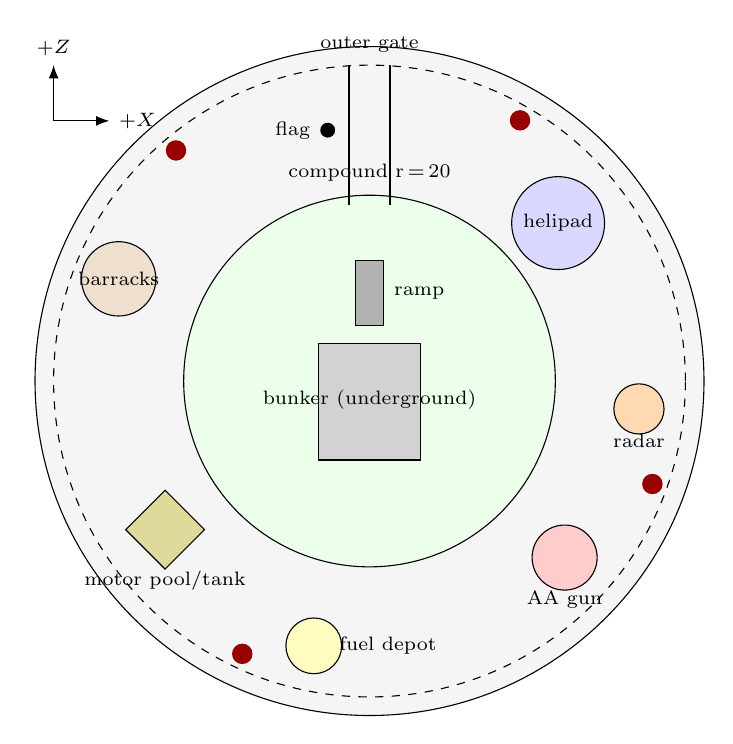
\begin{tikzpicture}[scale=0.118,font=\scriptsize]
  \draw[fill=black!4] (0,0) circle (36);
  \draw[dashed] (0,0) circle (34);
  \draw[fill=green!8,thin] (0,0) circle (20);
  \node[above] at (0,20.5) {compound r\,=\,20};
  % bunker footprint
  \draw[fill=gray!35] (-5.5,-8.5) rectangle (5.5,4);
  \node at (0,-2) {bunker (underground)};
  % ramp
  \draw[fill=gray!60] (-1.5,6) rectangle (1.5,13);
  \node[right] at (1.6,9.5) {ramp};
  % road
  \draw[thick] (-2.2,19) -- (-2.2,34) (2.2,19) -- (2.2,34);
  \node[above] at (0,34.3) {outer gate};
  % helipad
  \draw[fill=blue!15] (20.3,17) circle (5); \node at (20.3,17) {helipad};
  % radar
  \draw[fill=orange!30] (29,-3) circle (2.7); \node[below=2mm] at (29,-3) {radar};
  % AA gun
  \draw[fill=red!20] (21,-19) circle (3.5); \node[below=3mm] at (21,-19) {AA gun};
  % motor pool
  \draw[fill=olive!30,rotate around={45:(-22,-16)}] (-25,-19) rectangle (-19,-13); \node[below=4mm] at (-22,-16) {motor pool/tank};
  % barracks
  \draw[fill=brown!25] (-27,11) circle (4); \node at (-27,11) {barracks};
  % depot
  \draw[fill=yellow!25] (-6,-28.5) circle (3); \node[right=2mm] at (-6,-28.5) {fuel depot};
  % flag
  \fill (-4.5,27) circle (0.8); \node[left=1mm] at (-4.5,27) {flag};
  % towers
  \foreach \a in {60,130,245,340} {\fill[red!60!black] ({32.4*cos(\a)},{32.4*sin(\a)}) circle (1.1);}
  % north arrow
  \draw[-{Latex}] (-34,28) -- (-34,34) node[above] {$+Z$};
  \draw[-{Latex}] (-34,28) -- (-28,28) node[right] {$+X$};
\end{tikzpicture}
\caption{Plan view of the site (from \code{BaseLayout.h}; tower angles are measured from $+X$ towards $+Z$ as in
\code{Base.cpp}). Dark circles: the four guard towers at $r=32.4$\,m.}
\label{fig:plan}
\end{figure}

\subsection{The journey of one frame}
The report follows the data. A \emph{vertex} begins as a number in a unit primitive; the $T\,R\,S$ matrix of its part and the hierarchy above it place it in the world (Chapters~\ref{sec:builder}--\ref{sec:construction}); the view and projection matrices, clipping and the viewport turn
it into a pixel and a depth (Chapter~\ref{sec:geomchain}); the rasteriser interpolates its attributes (Chapter~\ref{sec:interp}); the fragment shader lights it (Chapter~\ref{sec:shading}); the reflection and post passes finish the image (Chapters~\ref{sec:reflection},~\ref{sec:pipeline}).
The scene is then rendered a second time as heat for each UAV; the computer vision turns that image into tracks (Chapter~\ref{sec:vision}) and the squad and rovers act on them (Chapters~\ref{sec:rover}, \ref{sec:squad}), which changes the next frame. A strip at the head of each
chapter marks its place in this pipeline; workbook screenshots accompany the objects they document.

\subsection{System overview}
Figure~\ref{fig:sysov}: the simulation updates a scene graph of primitives; the renderer draws it through the shading and post chain, and renders it again from each UAV's gimbal as a heat image for the vision. Audio and HUD read the game events.
\begin{figure}[h]
\centering
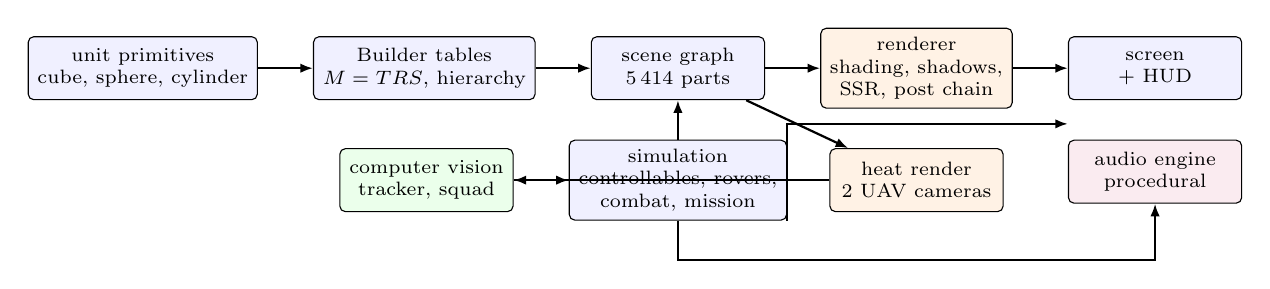
\begin{tikzpicture}[node distance=5mm and 7mm, every node/.style={font=\scriptsize},
  box/.style={draw,rounded corners=2pt,minimum height=8mm,minimum width=22mm,align=center,fill=blue!6},arr/.style={-{Latex[length=1.6mm]},thick}]
  \node[box] (prim) {unit primitives\\cube, sphere, cylinder};
  \node[box,right=of prim] (build) {Builder tables\\$M=TRS$, hierarchy};
  \node[box,right=of build] (scene) {scene graph\\\nLeaves{} parts};
  \node[box,below=of scene] (sim) {simulation\\controllables, rovers,\\combat, mission};
  \node[box,right=of scene,fill=orange!10] (rend) {renderer\\shading, shadows,\\SSR, post chain};
  \node[box,below=of rend,fill=orange!10] (heat) {heat render\\2 UAV cameras};
  \node[box,left=of sim,fill=green!8] (cv) {computer vision\\tracker, squad};
  \node[box,right=of rend] (screen) {screen\\+ HUD};
  \node[box,below=of screen,fill=purple!8] (audio) {audio engine\\procedural};
  \draw[arr] (prim)--(build); \draw[arr] (build)--(scene); \draw[arr] (scene)--(rend); \draw[arr] (rend)--(screen);
  \draw[arr] (scene)--(heat); \draw[arr] (heat)--(cv); \draw[arr] (cv)--(sim); \draw[arr] (sim)--(scene);
  \draw[arr] (sim.south) -- ++(0,-5mm) -| (audio.south); \draw[arr] (sim.south east) |- ([yshift=-3mm]screen.south west) ;
\end{tikzpicture}
\caption{System overview.}\label{fig:sysov}
\end{figure}

\paragraph{How to read this report.} Each chapter states the concept, the mathematics, the project's code (listings are lifted from the source by line range) and the tests or measurements.
Chapters~\ref{sec:prims}--\ref{sec:construction} cover geometry and object construction; \ref{sec:interp}--\ref{sec:pipeline} shading and the render pipeline; \ref{sec:rover} and \ref{sec:vision} the rover and the computer vision;
\ref{sec:v5plan}--\ref{sec:v5media} the game; the later chapters the machines, bunker, platform, tests and results; \ref{sec:daycycle}--\ref{sec:v6results} the v6 day cycle, soldiers, random routes, sensor model and their results. All numbers are generated from the program output.

% =====================================================================
\section{Primitives, Indexed Rendering and Memory}\label{sec:prims}
\pipestrip{1}
Every primitive is a list of unique vertices $(x,y,z,n_x,n_y,n_z)$, 24 bytes each, plus a triangle index list, wound counter-clockwise seen from outside so that \code{GL\_CCW} and back-face culling keep only outward faces. The resolution is $N=36$ slices, $\Delta\phi=10^\circ$. The generators in \code{src/primitives/} are the \emph{only} source of geometry, except the terrain disc (the cylinder cap subdivided into rings and lifted by a height field).

\subsection{Cube, sphere, cylinder, cone and frustum}
\textbf{Cube.} Each face has an outward normal $\vect n$ and in-plane axes $\vect u,\vect v$ with
$\vect u\times\vect v=\vect n$; its corners are
$\vect p_c=\tfrac12\vect n+\tfrac12 s_u\vect u+\tfrac12 s_v\vect v$ with
$(s_u,s_v)\in\{(-,-),(+,-),(+,+),(-,+)\}$, counter-clockwise about $\vect n$, split into $(0,1,2)$ and
$(0,2,3)$. A corner is stored once per face (its normal differs): 24 vertices, 36 indices, 12 triangles (T01--T03).

\textbf{Sphere.} With $r=0.5$, $\theta_k=k\pi/S$, $\phi_j=2\pi j/N$ ($S=18$, $N=36$):
$x=r\sin\theta_k\cos\phi_j$, $y=r\cos\theta_k$, $z=r\sin\theta_k\sin\phi_j$, $\vect n=\vect p/r$. Only the
northern hemisphere is computed; the southern half is its reflection $y\mapsto-y$. A reflection reverses orientation, so each mirrored triangle
$(a,b,c)$ is emitted as $(a',c',b')$. The shared equator gives $2+(S-1)N=614$ vertices and $2N(S-1)=1224$
triangles (T04--T06).

\textbf{Cylinder, cone, frustum.} The axis is the local $z$ axis, $z\in[-0.5,0.5]$. The side joins two rings,
\begin{equation}
  \vect p^{\,b}_j=(r_b\cos\phi_j,\,r_b\sin\phi_j,\,-0.5),\quad
  \vect p^{\,t}_j=(r_t\cos\phi_j,\,r_t\sin\phi_j,\,+0.5),\quad
  \vect n_j=\mathrm{normalize}(\cos\phi_j,\,\sin\phi_j,\,r_b-r_t),
\end{equation}
and each cap is a fan around its own centre. With $r_b=r_t=0.5$ this is the lab cylinder: $4N+2=146$ vertices,
$4N=144$ triangles. With $r_t=0$ the same routine yields the \textbf{cone} (109 vertices, 72 triangles; no degenerate triangles, T36); with $0<r_t<r_b$ and no caps it yields the
searchlight \textbf{frustum} (72 vertices, T10). Cones (pine whorls, missile noses; 259 instances in the export) thus need no extra generator.

\begin{figure}[h]
\centering
\picsheet{sheet_vertex_cube}{\linewidth}
\caption{\sheetcaption{sheet_vertex_cube}}
\end{figure}
\begin{figure}[h]
\centering
\picdia{A1_cube_vertices}{0.92\linewidth}
\caption{The cube: 24 vertices (4 per face with the face normal) and 36 indices; 720\,B indexed against 864\,B flat.}
\end{figure}
\begin{figure}[h]
\centering
\picdia{A2_sphere_rings}{0.92\linewidth}
\caption{The sphere: rings of 36 slices, normals equal to the normalised positions, the southern half mirrored.}
\end{figure}
\begin{figure}[h]
\centering
\picdia{A3_cylinder_cone}{0.92\linewidth}
\caption{Cylinder, cone and frustum from one generator.}
\end{figure}
\begin{figure}[h]
\centering
\picdia{A4_terrain_disc}{0.92\linewidth}
\caption{The terrain disc: ring structure (left) and the real triangles with the entrance-ramp hole (right).}
\end{figure}
\subsection{The generator code}
Listing~\ref{lst:Cube}: each face is a frame $(\vect n,\vect u,\vect v)$ with four counter-clockwise corners. Listing~\ref{lst:Sphere}: the northern hemisphere is generated ring by ring and mirrored. Listing~\ref{lst:Cylinder}: two rings joined by side quads with normals tilted by $r_b-r_t$, plus caps; a top radius of 0 gives the cone.
\lstCube
\lstSphere
\lstCylinder
\paragraph{The terrain disc.} The terrain is the cylinder cap subdivided into $R=130$ rings of $N=384$ slices ($1+RN=49\,921$ vertices, $N(2R-1)=99\,456$ triangles minus 2\,016 cut out for the entrance trench $=97\,440$, T13), radius 36\,m, each vertex lifted to
$y=h(x,z)$: rolling hills, a levelled bunker pad, a creek, a track, a berm and a mound over the bunker. Normals come from central differences of $h$.

\subsection{Indexed rendering and memory}
\sheetfig{s02_cube_indices}
\sheetfig{s06_geometry_stats}
\sheetfig{s06_charts}
Without indexing every triangle stores its three vertices (lab technique 1: 18 floats for a square); with
indexing, unique vertices go to the VBO and triangles reference them through the EBO (technique 2: 12 floats $+$ 6
indices). The VAO records \emph{location 0: offset 0, stride 24\,B} (position) and \emph{location 1: offset 12\,B}
(normal); one VAO+VBO+EBO per primitive is shared by every part. Memory per mesh is
$M_\text{flat}=3T\cdot 24$\,B and $M_\text{indexed}=24V+12T$\,B (Table~\ref{tab:memory}). The six meshes take \memIndexed\,B indexed against \memNonIndexed\,B non-indexed, dominated by the
terrain disc; they serve all \nLeaves{} parts. T12 checks that every indexed mesh is smaller than its flat version.

\begin{table}[h]
\centering\small
\caption{GPU meshes (from \code{build/scene\_export.json}). The terrain's vertex count (49\,921) is that of the 36\,m mesh (T13).}
\label{tab:memory}
% generated by report/gen_tables.py from build/scene_export.json -- do not edit
\begin{tabular}{@{}lrrrrrrr@{}}
\toprule
Mesh & $V$ & Indices & Triangles & Non-indexed (B) & Indexed (B) & Saving & Instances\\\midrule
Cube & 24 & 36 & 12 & 864 & 720 & 16.7\,\% & 2,231\\
Sphere & 614 & 3,672 & 1,224 & 88,128 & 29,424 & 66.6\,\% & 816\\
Cylinder & 146 & 432 & 144 & 10,368 & 5,232 & 49.5\,\% & 2,068\\
Cylinder (frustum) & 72 & 216 & 72 & 5,184 & 2,592 & 50.0\,\% & 3\\
Terrain disc & 49,921 & 292,320 & 97,440 & 7,015,680 & 2,367,384 & 66.3\,\% & 1\\
Cone & 109 & 216 & 72 & 5,184 & 3,480 & 32.9\,\% & 295\\
\midrule
Sum & & & & 7,125,408 & 2,408,832 & 66.2\,\% &\\
\bottomrule
\end{tabular}

\end{table}

\begin{figure}[h]
\centering
\picsheet{sheet_memory}{\linewidth}
\caption{\sheetcaption{sheet_memory}}
\end{figure}
\paragraph{Instancing and culling.} The grass is the unit cube drawn with \code{glDrawElementsInstanced} (per-instance buffer, \code{glVertexAttribDivisor}); the quality preset sets the count: LOW 14\,000, HIGH 35\,000,
ULTRA 140\,000, EPIC 450\,000 blades. Rain streaks, foliage cards and effect sprites use the same mechanism. Every pass culls parts whose bounding sphere $r=\tfrac12\sqrt{s_x^2+s_y^2+s_z^2}$ lies outside one of the six
frustum planes (Gribb--Hartmann, Chapter~\ref{sec:geomchain}).

\paragraph{Tests.} T01--T13 check counts, centring, normal length, winding, sphere reflection, cylinder
axis, index validity and the memory comparison (all \nTests{} tests: Section~\ref{sec:testing}).

% =====================================================================
\section{The Builder Table: One Row per Part}\label{sec:builder}
\pipestrip{2}
\emph{Concept.} An object is not a model file but a \emph{table}: one row per part, saying ``take this primitive, scale it, rotate it, move it'' (the $S,R,T$ table of the lab sheet). A part is a leaf of a scene graph; a group node carries only a transform and a name, and children are placed in the group's frame.

\subsection{One row, one part}
Table~\ref{tab:rows} shows real rows from \code{build/scene\_export.json}. The columns are the arguments of
\code{Builder::part} (Listing~\ref{lst:Part}): parent, name, primitive, scale $S$ (m), rotation $R$ (degrees, applied $R_y$, $R_x$, $R_z$), translation $T$ in the parent's frame, material and purpose.
\begin{table}[h]
\centering\footnotesize
\caption{Rows of the construction table (from the export). A cube is scaled to the box it should become; a cylinder's $z$ is its length.}\label{tab:rows}
\begin{tabular}{@{}llp{2.6cm}p{2.2cm}p{2.8cm}l@{}}
\toprule Part (id) & Primitive & $S$ & $R$ & $T$ & Parent\\\midrule
Hull core (TNK-02) & cube & $1.70,\,0.90,\,5.60$ & $0$ & $0,\,0.80,\,0$ & Hull\\
Track link L00 (TNK-42) & cube & $0.55,\,0.08,\,0.33$ & $0$ & $0,\,1.05,\,-2.80$ & Track L\\
Gatling barrel (AAG-30) & cylinder & $0.07,\,0.07,\,2.0$ & $0$ & $0,\,0.14,\,1.0$ & Barrel cluster\\
Blade 1 (HEL-31) & cube & $0.22,\,0.03,\,3.9$ & $0$ & $0,\,0,\,1.95$ & Blade 1 flap\\
Round nose (UAV-54) & cone & $0.022,\,0.022,\,0.04$ & $0$ & $0,\,0,\,0.105$ & Round\\
Wheel L (ROV-05) & cylinder & $0.16,\,0.16,\,0.07$ & $R_y=90$ & $0.25,\,0.08,\,-0.22$ & Target Rover\\\bottomrule
\end{tabular}
\end{table}

\lstPart

\subsection{From rows to matrices}
A leaf's local matrix is $M=T\,R_y\,R_x\,R_z\,S$ (Listing~\ref{lst:Transform}); its world matrix is the parent's world matrix times $M$, computed top-down once per frame (Listing~\ref{lst:UpdateNode}). The \code{explode} argument
multiplies the translation of every explodable node by $1+0.7\,e$ (Section~\ref{sec:transform}).
\lstTransform
\lstUpdateNode
\emph{Why $T\,R\,S$.} The primitive is a unit cube centred at the origin: $S$ makes the right box about its centre, $R$ tilts it about that centre, $T$ places it. In the
opposite order $T$ would be scaled and rotated as well.

\subsection{Naming and documentation}
Every node has a name, an owning object, a purpose and, if it moves, an \code{animation} text; the exporter writes them to JSON and the workbook reads them, so the report's part counts and hierarchy diagrams are never typed by hand.

% =====================================================================
\section{Transformations and Hierarchies}\label{sec:transform}
\pipestrip{2}
The model matrix of a node and its world matrix are
\begin{equation}
  M = T(\vect t)\,R_y(\psi)\,R_x(\theta)\,R_z(\varphi)\,S(\vect s),\qquad
  W_\text{node} = W_\text{parent}\,M ,
\end{equation}
\begin{equation}
  T=\begin{bmatrix}1&0&0&t_x\\0&1&0&t_y\\0&0&1&t_z\\0&0&0&1\end{bmatrix},\;
  S=\begin{bmatrix}s_x&0&0&0\\0&s_y&0&0\\0&0&s_z&0\\0&0&0&1\end{bmatrix},\;
  R_y(\psi)=\begin{bmatrix}\cos\psi&0&\sin\psi&0\\0&1&0&0\\-\sin\psi&0&\cos\psi&0\\0&0&0&1\end{bmatrix}.
\end{equation}
The primitive is scaled first, then rotated about its own centre, then placed; the other order would scale the
translation too (T14: $(1,0,0)\xrightarrow{S(2)}(2,0,0)\xrightarrow{R_z(90^\circ)}(0,2,0)\xrightarrow{T(1,2,3)}(1,4,3)$).
Normals use $(M^{-1})^T$ (T15, T16). A leaf inherits the product of all its ancestors' $M$: animation code writes only the \emph{local} transform of a few group nodes (a track link's translation, a blade's flap angle, a door's $x$ offset) and \code{Scene::updateWorld()}
recomputes all world matrices top-down in one pass. The pipeline of one vertex is
\begin{equation}
  \vect p_\text{clip}=P\,V\,W_\text{parent}\,T R S\,\vect p_\text{local}.
\end{equation}

\subsection{Worked $M=T\cdot R\cdot S$ examples}
\sheetfig{s04_inputs_blocks}
\sheetfig{s04_rows_error}
\sheetfig{s04_rows_m}
\sheetfig{s05_world_matrix}
Table~\ref{tab:mexamples} lists values copied from \code{build/scene\_export.json}; the workbook rebuilds
$T$, $R$, $S$ and $M$ for every part with cell formulas and checks them against the code. Three rows are expanded to full matrices below.

\begin{table}[h]
\centering\footnotesize
\setlength{\tabcolsep}{3pt}
\caption{Example parts. $S$ in metres, $R$ in degrees ($R_y,R_x,R_z$ order as in the code), $T$ in metres in the
parent's frame. The last column says which ancestor transform moves the part.}
\label{tab:mexamples}
\begin{tabular}{@{}p{2.5cm}l p{2.5cm} p{1.7cm} p{3.2cm} p{3.2cm}@{}}
\toprule
Part (id) & Prim. & $S$ & $R$ & $T$ & Driven by\\\midrule
Track link L17 (TNK-59) & cube & $0.55,\,0.08,\,0.33$ & $R_x=56.74$ & $0,\,0.8242,\,3.2181$ & arc-length parameter (every frame)\\
Track link L03 (TNK-45) & cube & $0.55,\,0.08,\,0.33$ & $0$ & $0,\,1.05,\,-1.7244$ & same; on the top run\\
Blade 1 (HEL-31) & cube & $0.22,\,0.03,\,3.9$ & $0$ & $0,\,0,\,1.95$ & flap node: $R_x=-\beta$, $R_z$=feather; spin node $R_y$\\
Gatling barrel 2 (AAG-31) & cyl. & $0.07,\,0.07,\,2$ & $0$ & $0.121,\,0.07,\,1$ & cluster node $R_z$ = spin angle\\
Array tile c2 r2 (RDR-58) & cube & $0.64,\,0.78,\,0.05$ & $R_y=15$ & $-1.294,\,0,\,0.17$ & azimuth / elevation nodes\\
Door leaf plate (BNK-97) & cube & $1.45,\,2.6,\,0.35$ & $0$ & $0,\,0,\,0$ & leaf node: $T_x=\pm1.5\,s(t)$\\
Wheel L (ROV-05) & cyl. & $0.16,\,0.16,\,0.07$ & $R_y=90$ & $0.25,\,0.08,\,-0.22$ & wheel node $R_z$ = roll angle\\
Missile fin (UAV-55) & cube & $0.002,\,0.03,\,0.03$ & $R_z=45$ & $0,\,0,\,-0.07$ & round node (hidden at launch)\\\bottomrule
\end{tabular}
\end{table}

\paragraph{Track link L17 (front arc).} $R_x(\varphi)$ turns the link's local $+y$ onto the outward
normal of the track path ($\varphi=56.74^\circ$, $\cos\varphi=0.548$, $\sin\varphi=0.836$):
\begin{equation}
M=\begin{bmatrix}0.55&0&0&0\\0&0.08\cos\varphi&-0.33\sin\varphi&0.8242\\0&0.08\sin\varphi&0.33\cos\varphi&3.2181\\0&0&0&1\end{bmatrix}
=\begin{bmatrix}0.55&0&0&0\\0&0.0439&-0.2760&0.8242\\0&0.0669&0.1810&3.2181\\0&0&0&1\end{bmatrix}
\end{equation}
which equals the exported \code{local\_matrix}.

\paragraph{Radar array tile c2 r2.} Column $k$ of 7 sits on an arc of radius $R_a=5$\,m at $\theta_k=(k-4)\cdot7.5^\circ$: $T_x=R_a\sin\theta_k$, $T_z=R_a(1-\cos\theta_k)$, $R_y=-\theta_k$ (for $k=2$: $T=(-1.294,0,0.17)$, $R_y=15^\circ$):
\begin{equation}
M=T R_y(15^\circ)S=\begin{bmatrix}0.64\cos15^\circ&0&0.05\sin15^\circ&-1.294\\0&0.78&0&0\\-0.64\sin15^\circ&0&0.05\cos15^\circ&0.17\\0&0&0&1\end{bmatrix}
=\begin{bmatrix}0.618&0&0.0129&-1.294\\0&0.78&0&0\\-0.166&0&0.0483&0.17\\0&0&0&1\end{bmatrix}.
\end{equation}

\paragraph{Rover wheel and why $R_z$ is the spin.} A cylinder (axis $z$) is scaled,
spun about its own axis by $R_z$, \emph{then} turned onto the $x$ axis by $R_y(90^\circ)$:
\begin{equation}
M_\text{wheel}=T\,R_y(90^\circ)\,R_z(\omega t)\,S=
\begin{bmatrix}0&0&0.07&0.25\\0&0.16&0&0.08\\-0.16&0&0&-0.22\\0&0&0&1\end{bmatrix}\quad(\omega t=0).
\end{equation}

\paragraph{A deep chain: the helicopter blade.}
\begin{equation}
W_\text{blade}=M_\text{root}M_\text{body}M_\text{head}M_\text{tpp}(\tau_f,\tau_l)\,R_y(\Psi)\,M_\text{pivot}(\psi_i)\,
M_\text{flap}(-\beta,\vartheta)\,M_\text{blade},
\end{equation}
with the root carrying position and yaw, the body the spring-damped pitch and roll, the tip-path-plane node
the cyclic tilts $(\tau_f,\tau_l)$, the spin node the azimuth $\Psi$, the pivot the blade's $72^\circ$ offset,
and the flap node the flap $\beta$ and collective feather $\vartheta$ (Section~\ref{sec:control}).

\begin{figure}[h]
\centering
\picdia{A5_trs_worked_example}{0.92\linewidth}
\caption{Worked $T\,R\,S$ example for one real part (from the program's matrices).}
\end{figure}
\begin{figure}[h]
\centering
\picdia{A6_hierarchy_uav}{0.92\linewidth}
\caption{Hierarchy of the UAV with the world-matrix chain of the searchlight.}
\end{figure}
\begin{figure}[h]
\centering
\picdia{A6_hierarchy_tank}{0.92\linewidth}
\caption{Hierarchy of the tank.}
\end{figure}
\subsection{The explode view}
Key \texttt{E} pushes the parts of the bunker, UAV and rover apart: \code{updateNode()} multiplies the translation of every explodable node by $1+0.7\,e$ with $e\in[0,1]$ eased in by the
application. Only local translations are scaled, so children follow their parent's scaled position and a sub-assembly (a wheel with its hub) opens up as a hierarchy rather than
a cloud. The tank, helicopter, AA gun, radar and base are not exploded: their own animation code writes their transforms every frame.

\begin{figure}[h]
\centering
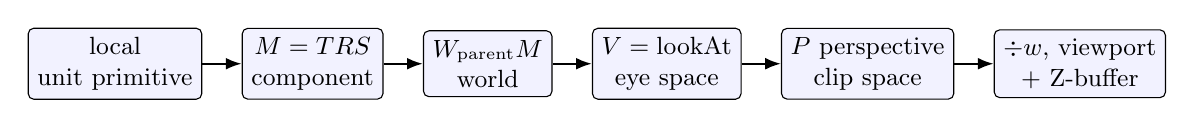
\begin{tikzpicture}[node distance=4mm and 5mm, every node/.style={font=\small},
  box/.style={draw,rounded corners=2pt,minimum height=6.5mm,align=center,fill=blue!5},
  arr/.style={-{Latex[length=2mm]},thick}]
  \node[box] (a) {local\\unit primitive};
  \node[box,right=of a] (b) {$M=TRS$\\component};
  \node[box,right=of b] (c) {$W_\text{parent}M$\\world};
  \node[box,right=of c] (d) {$V=\text{lookAt}$\\eye space};
  \node[box,right=of d] (e) {$P$ perspective\\clip space};
  \node[box,right=of e] (f) {$\div w$, viewport\\+ Z-buffer};
  \foreach \x/\y in {a/b,b/c,c/d,d/e,e/f} \draw[arr] (\x)--(\y);
\end{tikzpicture}
\caption{Vertex pipeline: $\vect p_\text{clip}=P\,V\,W_\text{parent}\,T R S\,\vect p_\text{local}$.}
\label{fig:transform}
\end{figure}

\paragraph{Local axes.} Key \texttt{H} draws the local axes of the UAV hierarchy (UAV, gimbal yaw, gimbal pitch) and the
rover. The searchlight shows why the order matters:
$W_\text{lamp}=W_\text{UAV}\,M_\text{yaw}(\psi_g)\,M_\text{pitch}(\theta_g)$; the spotlight sits at the lens of
$W_\text{lamp}$ and points along its local $+z$ (T21: the lamp moved 0.776\,m when the body moved 0.750\,m).

% =====================================================================
\section{The Objects, Part by Part}\label{sec:construction}
\pipestrip{2}
A composite object is a small scene graph: leaves draw one primitive with their own $S,R,T$; group nodes carry a transform and a name. Table~\ref{tab:parts} is
generated from the export: the scene holds \nLeaves{} leaf parts in \nObjects{} objects. T38 checks that every
leaf is a cube, sphere, cylinder or cone; T70/T67/T96/T99 check each object for ``primitives only, every node named''.

\begin{table}[h]
\centering\small
\caption{Parts per composite object, generated from \code{build/scene\_export.json}. Depth is the deepest group
level. The \emph{Target Rover} row counts all three intruders (\partsRover{} parts each). }
\label{tab:parts}
% generated by report/gen_tables.py from build/scene_export.json -- do not edit
\begin{tabular}{@{}lrrrp{4.6cm}l@{}}
\toprule
Object (export name) & Parts & Groups & Depth & Cube / Sphere / Cylinder / Cone / Frustum & Shading\\\midrule
Terrain & 1 & 1 & 1 & 1 height-field disc & Gouraud 1\\
Backdrop & 120 & 47 & 3 & 0 / 24 / 10 / 86 / 0 & Gouraud 120\\
Environment & 652 & 89 & 3 & 46 / 201 / 237 / 168 / 0 & Gouraud 652\\
Command Bunker & 400 & 17 & 3 & 291 / 19 / 90 / 0 / 0 & Flat 400\\
Autonomous UAV & 158 & 34 & 3 & 68 / 26 / 54 / 8 / 2 & Phong 156,\allowbreak{} Additive beam 2\\
Base & 1253 & 33 & 3 & 558 / 41 / 654 / 0 / 0 & Flat 616,\allowbreak{} Gouraud 637\\
Target Rover & 156 & 12 & 2 & 36 / 72 / 48 / 0 / 0 & Phong 156\\
Main Battle Tank & 255 & 29 & 5 & 170 / 5 / 80 / 0 / 0 & Phong 255\\
Scout Helicopter & 91 & 19 & 7 & 40 / 21 / 28 / 1 / 1 & Phong 90,\allowbreak{} Additive beam 1\\
AA Gatling Gun & 78 & 5 & 4 & 19 / 5 / 54 / 0 / 0 & Phong 78\\
Air-defence radar & 108 & 4 & 4 & 62 / 3 / 42 / 1 / 0 & Phong 108\\
SAM launcher & 112 & 9 & 4 & 74 / 5 / 32 / 1 / 0 & Phong 112\\
MLRS rocket truck & 136 & 22 & 4 & 45 / 9 / 76 / 6 / 0 & Phong 136\\
Main Battle Tank 2 & 255 & 29 & 5 & 170 / 5 / 80 / 0 / 0 & Phong 255\\
Main Battle Tank 3 & 255 & 29 & 5 & 170 / 5 / 80 / 0 / 0 & Phong 255\\
Ammunition bunker & 43 & 2 & 2 & 19 / 10 / 14 / 0 / 0 & Gouraud 43\\
Camp camouflage & 658 & 21 & 2 & 277 / 48 / 309 / 24 / 0 & Gouraud 658\\
Boom barrier & 20 & 2 & 2 & 17 / 2 / 1 / 0 / 0 & Gouraud 20\\
Windsock & 15 & 7 & 7 & 1 / 0 / 14 / 0 / 0 & Gouraud 15\\
Flag & 47 & 14 & 14 & 40 / 2 / 5 / 0 / 0 & Gouraud 47\\
Soldier 1 & 75 & 20 & 7 & 16 / 39 / 20 / 0 / 0 & Phong 75\\
Soldier 2 & 75 & 20 & 7 & 16 / 39 / 20 / 0 / 0 & Phong 75\\
Soldier 3 & 75 & 20 & 7 & 16 / 39 / 20 / 0 / 0 & Phong 75\\
Soldier 4 & 75 & 20 & 7 & 16 / 39 / 20 / 0 / 0 & Phong 75\\
Soldier 5 & 75 & 20 & 7 & 16 / 39 / 20 / 0 / 0 & Phong 75\\
Soldier 6 & 75 & 20 & 7 & 16 / 39 / 20 / 0 / 0 & Phong 75\\
Soldier 7 & 75 & 20 & 7 & 16 / 39 / 20 / 0 / 0 & Phong 75\\
Soldier 8 & 75 & 20 & 7 & 16 / 39 / 20 / 0 / 0 & Phong 75\\
Sky Clock & 1 & 1 & 1 & 0 / 1 / 0 / 0 / 0 & Gouraud 1\\
\midrule
Total & 5414 & 586 & & &\\
\bottomrule
\end{tabular}

\end{table}

\noindent The hierarchy diagrams are generated from the export: \emph{[n]} is the number of leaf
parts below a node, ``$\times k$'' collapses $k$ identical sibling groups, and italic lines summarise leaves directly under a group.

% ---------------------------------------------------------------------
\begin{figure}[h]
\centering
\picsheet{sheet_hierarchy}{\linewidth}
\caption{\sheetcaption{sheet_hierarchy}}
\end{figure}
\subsection{Underground command bunker}
\sheetfig{s03_primitive_mix}
\sheetfig{s03_bunker}
The bunker (\partsBunker{} parts, Flat shading) is underground: an entrance trench follows the vehicle track down a 7\,m ramp
($z=13\to6$) to the blast-door plane at $z=4$; behind it a tunnel leads to the command centre (CIC), a bunk room, a generator room and an emergency shaft with a ladder to a surface
hatch. All rooms share the floor level $y=-3.4$\,m; the terrain stays at least 0.15\,m above the roof slab (T60). Consoles in the CIC use the procedural \emph{Screen} surface. The two door leaves and two beacon spinners are animated (Section~\ref{sec:control}).

\begin{figure}[h]
\centering
\begin{minipage}[t]{0.52\linewidth}\vspace{0pt}% generated by report/gen_tables.py from build/scene_export.json -- do not edit
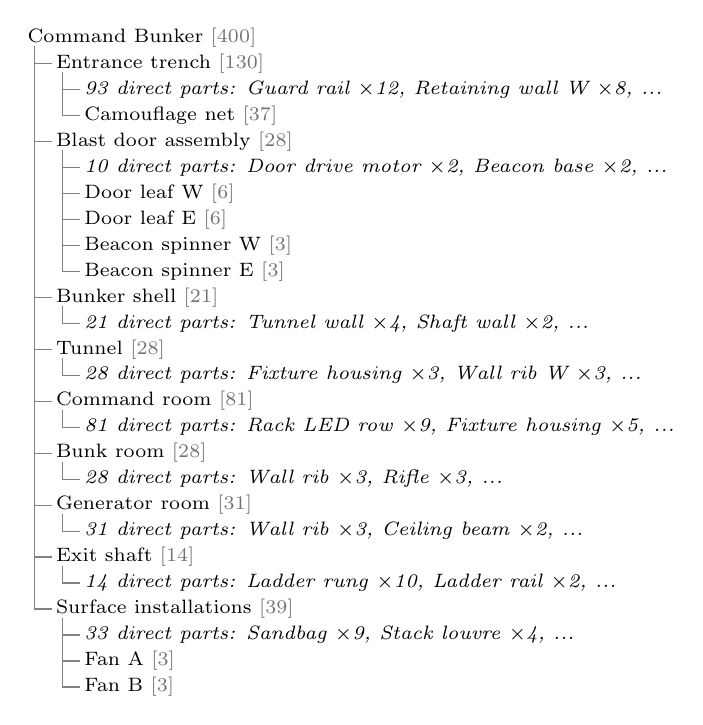
\begin{tikzpicture}[x=0.36cm,y=-0.33cm,font=\scriptsize]
\node[anchor=west,inner sep=0pt] (n0) at (0,0) {Command Bunker \textcolor{black!55}{[400]}};
\node[anchor=west,inner sep=0pt] (n1) at (1,1) {Entrance trench \textcolor{black!55}{[130]}};
\draw[black!50,thin] (0.25,0.35) |- (0.88,1);
\node[anchor=west,inner sep=0pt] (n2) at (2,2) {\textit{93 direct parts: Guard rail $\times$12, Retaining wall W $\times$8, ...}};
\draw[black!50,thin] (1.25,1.35) |- (1.88,2);
\node[anchor=west,inner sep=0pt] (n3) at (2,3) {Camouflage net \textcolor{black!55}{[37]}};
\draw[black!50,thin] (1.25,1.35) |- (1.88,3);
\node[anchor=west,inner sep=0pt] (n4) at (1,4) {Blast door assembly \textcolor{black!55}{[28]}};
\draw[black!50,thin] (0.25,0.35) |- (0.88,4);
\node[anchor=west,inner sep=0pt] (n5) at (2,5) {\textit{10 direct parts: Door drive motor $\times$2, Beacon base $\times$2, ...}};
\draw[black!50,thin] (1.25,4.35) |- (1.88,5);
\node[anchor=west,inner sep=0pt] (n6) at (2,6) {Door leaf W \textcolor{black!55}{[6]}};
\draw[black!50,thin] (1.25,4.35) |- (1.88,6);
\node[anchor=west,inner sep=0pt] (n7) at (2,7) {Door leaf E \textcolor{black!55}{[6]}};
\draw[black!50,thin] (1.25,4.35) |- (1.88,7);
\node[anchor=west,inner sep=0pt] (n8) at (2,8) {Beacon spinner W \textcolor{black!55}{[3]}};
\draw[black!50,thin] (1.25,4.35) |- (1.88,8);
\node[anchor=west,inner sep=0pt] (n9) at (2,9) {Beacon spinner E \textcolor{black!55}{[3]}};
\draw[black!50,thin] (1.25,4.35) |- (1.88,9);
\node[anchor=west,inner sep=0pt] (n10) at (1,10) {Bunker shell \textcolor{black!55}{[21]}};
\draw[black!50,thin] (0.25,0.35) |- (0.88,10);
\node[anchor=west,inner sep=0pt] (n11) at (2,11) {\textit{21 direct parts: Tunnel wall $\times$4, Shaft wall $\times$2, ...}};
\draw[black!50,thin] (1.25,10.35) |- (1.88,11);
\node[anchor=west,inner sep=0pt] (n12) at (1,12) {Tunnel \textcolor{black!55}{[28]}};
\draw[black!50,thin] (0.25,0.35) |- (0.88,12);
\node[anchor=west,inner sep=0pt] (n13) at (2,13) {\textit{28 direct parts: Fixture housing $\times$3, Wall rib W $\times$3, ...}};
\draw[black!50,thin] (1.25,12.35) |- (1.88,13);
\node[anchor=west,inner sep=0pt] (n14) at (1,14) {Command room \textcolor{black!55}{[81]}};
\draw[black!50,thin] (0.25,0.35) |- (0.88,14);
\node[anchor=west,inner sep=0pt] (n15) at (2,15) {\textit{81 direct parts: Rack LED row $\times$9, Fixture housing $\times$5, ...}};
\draw[black!50,thin] (1.25,14.35) |- (1.88,15);
\node[anchor=west,inner sep=0pt] (n16) at (1,16) {Bunk room \textcolor{black!55}{[28]}};
\draw[black!50,thin] (0.25,0.35) |- (0.88,16);
\node[anchor=west,inner sep=0pt] (n17) at (2,17) {\textit{28 direct parts: Wall rib $\times$3, Rifle $\times$3, ...}};
\draw[black!50,thin] (1.25,16.35) |- (1.88,17);
\node[anchor=west,inner sep=0pt] (n18) at (1,18) {Generator room \textcolor{black!55}{[31]}};
\draw[black!50,thin] (0.25,0.35) |- (0.88,18);
\node[anchor=west,inner sep=0pt] (n19) at (2,19) {\textit{31 direct parts: Wall rib $\times$3, Ceiling beam $\times$2, ...}};
\draw[black!50,thin] (1.25,18.35) |- (1.88,19);
\node[anchor=west,inner sep=0pt] (n20) at (1,20) {Exit shaft \textcolor{black!55}{[14]}};
\draw[black!50,thin] (0.25,0.35) |- (0.88,20);
\node[anchor=west,inner sep=0pt] (n21) at (2,21) {\textit{14 direct parts: Ladder rung $\times$10, Ladder rail $\times$2, ...}};
\draw[black!50,thin] (1.25,20.35) |- (1.88,21);
\node[anchor=west,inner sep=0pt] (n22) at (1,22) {Surface installations \textcolor{black!55}{[39]}};
\draw[black!50,thin] (0.25,0.35) |- (0.88,22);
\node[anchor=west,inner sep=0pt] (n23) at (2,23) {\textit{33 direct parts: Sandbag $\times$9, Stack louvre $\times$4, ...}};
\draw[black!50,thin] (1.25,22.35) |- (1.88,23);
\node[anchor=west,inner sep=0pt] (n24) at (2,24) {Fan A \textcolor{black!55}{[3]}};
\draw[black!50,thin] (1.25,22.35) |- (1.88,24);
\node[anchor=west,inner sep=0pt] (n25) at (2,25) {Fan B \textcolor{black!55}{[3]}};
\draw[black!50,thin] (1.25,22.35) |- (1.88,25);
\end{tikzpicture}
\end{minipage}\hfill
\begin{minipage}[t]{0.44\linewidth}\vspace{0pt}
\footnotesize
\begin{tabular}{@{}ll@{}}\toprule
Floor/ceiling & $-3.4$\,m / $-0.8$\,m\\
Ramp & $z$ 13 $\to$ 6, 3\,m wide\\
Door plane & $z=4$, opening $2.6\times2.6$\,m\\
Footprint & $x\in[-5.5,5.5]$, $z\in[-8.5,4]$\\
Walk floors / walls & 12 / 36 boxes (T69)\\
Indoor volumes & 5 (T69)\\
Shading & Flat, all leaves (T67)\\\bottomrule
\end{tabular}
\end{minipage}
\caption{Bunker hierarchy (from the export) and key dimensions (\code{BaseLayout.h}, T67--T69).}
\label{fig:tree-bunker}
\end{figure}

% ---------------------------------------------------------------------
\subsection{The base apron}
The apron (r $\approx$ 20--36\,m) is built by \code{Base.cpp}: \partsBase{} static parts (Flat/Gouraud). It holds the HESCO perimeter (204 cells) with
wire coils, four guard towers at $r=32.4$\,m, the outer gate, road, helipad, motor pool, fuel depot, three Quonset barracks, and the sand-bag rings around the AA-gun
and radar pads. T72 checks that the wall is closed except for one 9--11\,m gate gap; T71 that no part
intersects another object's pad; T77 that nothing is an occluder and every part lies inside $r=36$\,m.

\begin{figure}[h]
\centering
\begin{minipage}[t]{0.56\linewidth}\vspace{0pt}% generated by report/gen_tables.py from build/scene_export.json -- do not edit
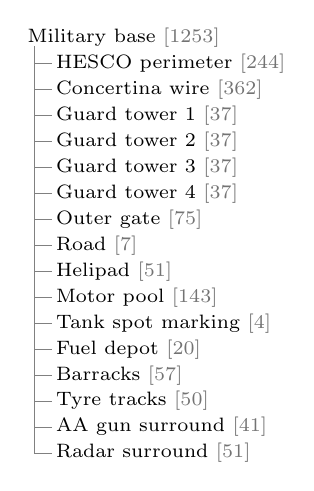
\begin{tikzpicture}[x=0.36cm,y=-0.33cm,font=\scriptsize]
\node[anchor=west,inner sep=0pt] (n0) at (0,0) {Military base \textcolor{black!55}{[1253]}};
\node[anchor=west,inner sep=0pt] (n1) at (1,1) {HESCO perimeter \textcolor{black!55}{[244]}};
\draw[black!50,thin] (0.25,0.35) |- (0.88,1);
\node[anchor=west,inner sep=0pt] (n2) at (1,2) {Concertina wire \textcolor{black!55}{[362]}};
\draw[black!50,thin] (0.25,0.35) |- (0.88,2);
\node[anchor=west,inner sep=0pt] (n3) at (1,3) {Guard tower 1 \textcolor{black!55}{[37]}};
\draw[black!50,thin] (0.25,0.35) |- (0.88,3);
\node[anchor=west,inner sep=0pt] (n4) at (1,4) {Guard tower 2 \textcolor{black!55}{[37]}};
\draw[black!50,thin] (0.25,0.35) |- (0.88,4);
\node[anchor=west,inner sep=0pt] (n5) at (1,5) {Guard tower 3 \textcolor{black!55}{[37]}};
\draw[black!50,thin] (0.25,0.35) |- (0.88,5);
\node[anchor=west,inner sep=0pt] (n6) at (1,6) {Guard tower 4 \textcolor{black!55}{[37]}};
\draw[black!50,thin] (0.25,0.35) |- (0.88,6);
\node[anchor=west,inner sep=0pt] (n7) at (1,7) {Outer gate \textcolor{black!55}{[75]}};
\draw[black!50,thin] (0.25,0.35) |- (0.88,7);
\node[anchor=west,inner sep=0pt] (n8) at (1,8) {Road \textcolor{black!55}{[7]}};
\draw[black!50,thin] (0.25,0.35) |- (0.88,8);
\node[anchor=west,inner sep=0pt] (n9) at (1,9) {Helipad \textcolor{black!55}{[51]}};
\draw[black!50,thin] (0.25,0.35) |- (0.88,9);
\node[anchor=west,inner sep=0pt] (n10) at (1,10) {Motor pool \textcolor{black!55}{[143]}};
\draw[black!50,thin] (0.25,0.35) |- (0.88,10);
\node[anchor=west,inner sep=0pt] (n11) at (1,11) {Tank spot marking \textcolor{black!55}{[4]}};
\draw[black!50,thin] (0.25,0.35) |- (0.88,11);
\node[anchor=west,inner sep=0pt] (n12) at (1,12) {Fuel depot \textcolor{black!55}{[20]}};
\draw[black!50,thin] (0.25,0.35) |- (0.88,12);
\node[anchor=west,inner sep=0pt] (n13) at (1,13) {Barracks \textcolor{black!55}{[57]}};
\draw[black!50,thin] (0.25,0.35) |- (0.88,13);
\node[anchor=west,inner sep=0pt] (n14) at (1,14) {Tyre tracks \textcolor{black!55}{[50]}};
\draw[black!50,thin] (0.25,0.35) |- (0.88,14);
\node[anchor=west,inner sep=0pt] (n15) at (1,15) {AA gun surround \textcolor{black!55}{[41]}};
\draw[black!50,thin] (0.25,0.35) |- (0.88,15);
\node[anchor=west,inner sep=0pt] (n16) at (1,16) {Radar surround \textcolor{black!55}{[51]}};
\draw[black!50,thin] (0.25,0.35) |- (0.88,16);
\end{tikzpicture}
\end{minipage}\hfill
\begin{minipage}[t]{0.40\linewidth}\vspace{0pt}
\captionsetup{type=figure}
\picfour{base_gate}{\linewidth}
\end{minipage}
\caption{Base hierarchy (left, from the export; the figure ``base\_gate'' (right) shows the outer gate with boom
barrier, booth and towers).}
\end{figure}

% ---------------------------------------------------------------------
\subsection{UAV with launcher rails}
\sheetfig{s03_uav}
The quadcopter (\partsUav{} parts, Phong) has a fuselage, canopy, four rotors, landing gear, LEDs, and the two-axis gimbal
\emph{body $\to$ gimbal yaw $\to$ gimbal pitch $\to$ \{lamp, lens, thermal camera, light frustum\}} shared by the thermal
tracker and the searchlight. Two \emph{launcher rails} (14 parts each) carry two missiles apiece (cylinder body, cone nose, four fins); a round is hidden on launch and
returns after the 10\,s reload (Section~\ref{sec:game}). Rotor-blur discs are translucent ($\alpha<1$, no shadow).

% ---------------------------------------------------------------------
\subsection{Intruder rover}
\sheetfig{s03_rover}
Each of the three intruders is a six-wheeled UGV with \partsRover{} parts: chassis, hull, motor box, six
cylinder wheels (axis turned onto $x$ by $R_y(90^\circ)$, spin $=R_z$), sphere hubs, five IR line sensors and a rotating
scanner. The motor box is the hottest part (thermal value 0.97), which the tracker locks on. The rovers share geometry with distinct part ids (\code{ROV-07}, \code{ROV2-07}, \code{ROV3-07}); a destroyed rover's parts become rigid debris (Section~\ref{sec:game}).

\begin{figure}[h]
\centering
\picsheet{sheet_construction_tank}{\linewidth}
\caption{\sheetcaption{sheet_construction_tank}}
\end{figure}
% ---------------------------------------------------------------------
\subsection{Main battle tank with 80 animated track links}
\sheetfig{s05_tank_chain}
\sheetfig{s03_tank_material}
The tank (\partsTank{} parts, Phong) parks at the motor pool facing the road. The hull carries plates, skirts and lights; the turret a cupola with a machine gun and smoke launchers; the gun is
\emph{gun pitch $\to$ barrel recoil $\to$ barrel, fume extractor, muzzle brake}. Each track has
$40$ link cubes ($\nTrackLinks$ in total) plus seven road wheels, sprocket, idler and rollers. Link
transforms are set each frame from the arc length along a closed stadium-shaped
path (Section~\ref{sec:control}); T80 checks that all 80 links stay on the path (max distance $0$\,m).

\begin{figure}[h]
\centering
\begin{minipage}[t]{0.31\linewidth}\vspace{0pt}% generated by report/gen_tables.py from build/scene_export.json -- do not edit
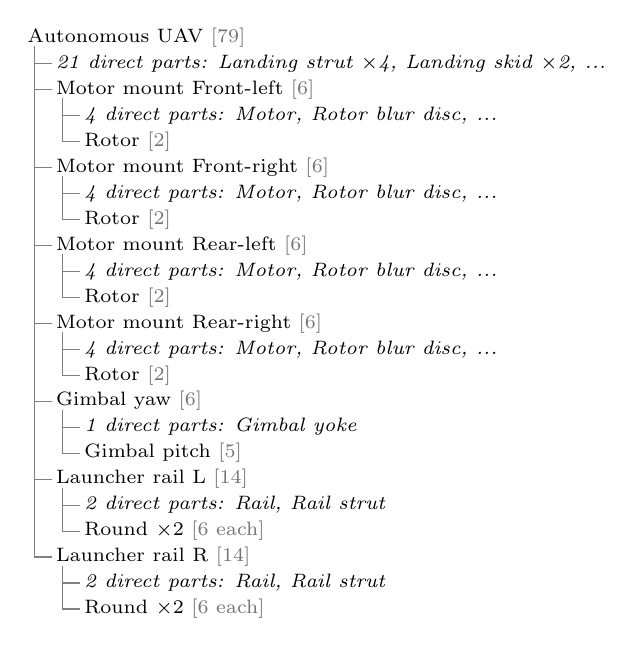
\begin{tikzpicture}[x=0.36cm,y=-0.33cm,font=\scriptsize]
\node[anchor=west,inner sep=0pt] (n0) at (0,0) {Autonomous UAV \textcolor{black!55}{[79]}};
\node[anchor=west,inner sep=0pt] (n1) at (1,1) {\textit{21 direct parts: Landing strut $\times$4, Landing skid $\times$2, ...}};
\draw[black!50,thin] (0.25,0.35) |- (0.88,1);
\node[anchor=west,inner sep=0pt] (n2) at (1,2) {Motor mount Front-left \textcolor{black!55}{[6]}};
\draw[black!50,thin] (0.25,0.35) |- (0.88,2);
\node[anchor=west,inner sep=0pt] (n3) at (2,3) {\textit{4 direct parts: Motor, Rotor blur disc, ...}};
\draw[black!50,thin] (1.25,2.35) |- (1.88,3);
\node[anchor=west,inner sep=0pt] (n4) at (2,4) {Rotor \textcolor{black!55}{[2]}};
\draw[black!50,thin] (1.25,2.35) |- (1.88,4);
\node[anchor=west,inner sep=0pt] (n5) at (1,5) {Motor mount Front-right \textcolor{black!55}{[6]}};
\draw[black!50,thin] (0.25,0.35) |- (0.88,5);
\node[anchor=west,inner sep=0pt] (n6) at (2,6) {\textit{4 direct parts: Motor, Rotor blur disc, ...}};
\draw[black!50,thin] (1.25,5.35) |- (1.88,6);
\node[anchor=west,inner sep=0pt] (n7) at (2,7) {Rotor \textcolor{black!55}{[2]}};
\draw[black!50,thin] (1.25,5.35) |- (1.88,7);
\node[anchor=west,inner sep=0pt] (n8) at (1,8) {Motor mount Rear-left \textcolor{black!55}{[6]}};
\draw[black!50,thin] (0.25,0.35) |- (0.88,8);
\node[anchor=west,inner sep=0pt] (n9) at (2,9) {\textit{4 direct parts: Motor, Rotor blur disc, ...}};
\draw[black!50,thin] (1.25,8.35) |- (1.88,9);
\node[anchor=west,inner sep=0pt] (n10) at (2,10) {Rotor \textcolor{black!55}{[2]}};
\draw[black!50,thin] (1.25,8.35) |- (1.88,10);
\node[anchor=west,inner sep=0pt] (n11) at (1,11) {Motor mount Rear-right \textcolor{black!55}{[6]}};
\draw[black!50,thin] (0.25,0.35) |- (0.88,11);
\node[anchor=west,inner sep=0pt] (n12) at (2,12) {\textit{4 direct parts: Motor, Rotor blur disc, ...}};
\draw[black!50,thin] (1.25,11.35) |- (1.88,12);
\node[anchor=west,inner sep=0pt] (n13) at (2,13) {Rotor \textcolor{black!55}{[2]}};
\draw[black!50,thin] (1.25,11.35) |- (1.88,13);
\node[anchor=west,inner sep=0pt] (n14) at (1,14) {Gimbal yaw \textcolor{black!55}{[6]}};
\draw[black!50,thin] (0.25,0.35) |- (0.88,14);
\node[anchor=west,inner sep=0pt] (n15) at (2,15) {\textit{1 direct parts: Gimbal yoke}};
\draw[black!50,thin] (1.25,14.35) |- (1.88,15);
\node[anchor=west,inner sep=0pt] (n16) at (2,16) {Gimbal pitch \textcolor{black!55}{[5]}};
\draw[black!50,thin] (1.25,14.35) |- (1.88,16);
\node[anchor=west,inner sep=0pt] (n17) at (1,17) {Launcher rail L \textcolor{black!55}{[14]}};
\draw[black!50,thin] (0.25,0.35) |- (0.88,17);
\node[anchor=west,inner sep=0pt] (n18) at (2,18) {\textit{2 direct parts: Rail, Rail strut}};
\draw[black!50,thin] (1.25,17.35) |- (1.88,18);
\node[anchor=west,inner sep=0pt] (n19) at (2,19) {Round $\times$2 \textcolor{black!55}{[6 each]}};
\draw[black!50,thin] (1.25,17.35) |- (1.88,19);
\node[anchor=west,inner sep=0pt] (n20) at (1,20) {Launcher rail R \textcolor{black!55}{[14]}};
\draw[black!50,thin] (0.25,0.35) |- (0.88,20);
\node[anchor=west,inner sep=0pt] (n21) at (2,21) {\textit{2 direct parts: Rail, Rail strut}};
\draw[black!50,thin] (1.25,20.35) |- (1.88,21);
\node[anchor=west,inner sep=0pt] (n22) at (2,22) {Round $\times$2 \textcolor{black!55}{[6 each]}};
\draw[black!50,thin] (1.25,20.35) |- (1.88,22);
\end{tikzpicture}
\end{minipage}\hfill
\begin{minipage}[t]{0.31\linewidth}\vspace{0pt}% generated by report/gen_tables.py from build/scene_export.json -- do not edit
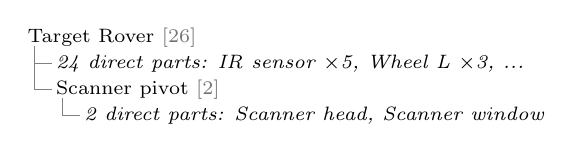
\begin{tikzpicture}[x=0.36cm,y=-0.33cm,font=\scriptsize]
\node[anchor=west,inner sep=0pt] (n0) at (0,0) {Target Rover \textcolor{black!55}{[26]}};
\node[anchor=west,inner sep=0pt] (n1) at (1,1) {\textit{24 direct parts: IR sensor $\times$5, Wheel L $\times$3, ...}};
\draw[black!50,thin] (0.25,0.35) |- (0.88,1);
\node[anchor=west,inner sep=0pt] (n2) at (1,2) {Scanner pivot \textcolor{black!55}{[2]}};
\draw[black!50,thin] (0.25,0.35) |- (0.88,2);
\node[anchor=west,inner sep=0pt] (n3) at (2,3) {\textit{2 direct parts: Scanner head, Scanner window}};
\draw[black!50,thin] (1.25,2.35) |- (1.88,3);
\end{tikzpicture}
\end{minipage}\hfill
\begin{minipage}[t]{0.35\linewidth}\vspace{0pt}% generated by report/gen_tables.py from build/scene_export.json -- do not edit
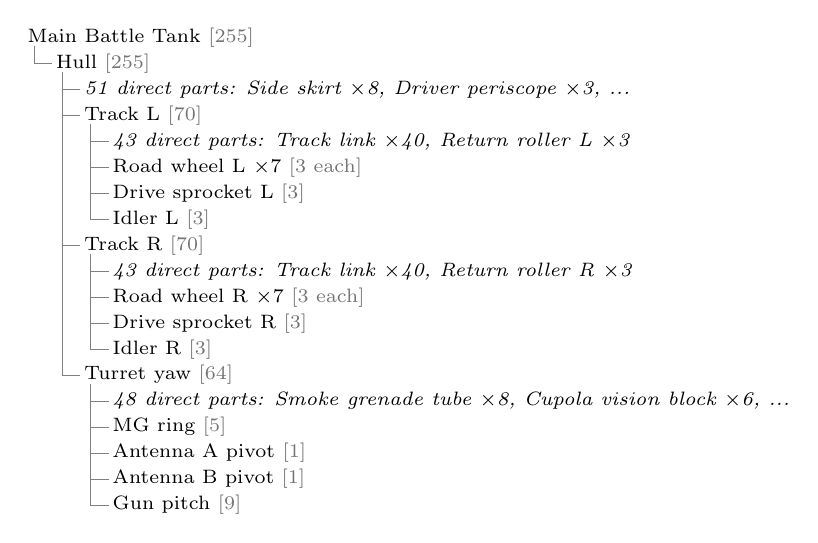
\begin{tikzpicture}[x=0.36cm,y=-0.33cm,font=\scriptsize]
\node[anchor=west,inner sep=0pt] (n0) at (0,0) {Main Battle Tank \textcolor{black!55}{[255]}};
\node[anchor=west,inner sep=0pt] (n1) at (1,1) {Hull \textcolor{black!55}{[255]}};
\draw[black!50,thin] (0.25,0.35) |- (0.88,1);
\node[anchor=west,inner sep=0pt] (n2) at (2,2) {\textit{51 direct parts: Side skirt $\times$8, Driver periscope $\times$3, ...}};
\draw[black!50,thin] (1.25,1.35) |- (1.88,2);
\node[anchor=west,inner sep=0pt] (n3) at (2,3) {Track L \textcolor{black!55}{[70]}};
\draw[black!50,thin] (1.25,1.35) |- (1.88,3);
\node[anchor=west,inner sep=0pt] (n4) at (3,4) {\textit{43 direct parts: Track link $\times$40, Return roller L $\times$3}};
\draw[black!50,thin] (2.25,3.35) |- (2.88,4);
\node[anchor=west,inner sep=0pt] (n5) at (3,5) {Road wheel L $\times$7 \textcolor{black!55}{[3 each]}};
\draw[black!50,thin] (2.25,3.35) |- (2.88,5);
\node[anchor=west,inner sep=0pt] (n6) at (3,6) {Drive sprocket L \textcolor{black!55}{[3]}};
\draw[black!50,thin] (2.25,3.35) |- (2.88,6);
\node[anchor=west,inner sep=0pt] (n7) at (3,7) {Idler L \textcolor{black!55}{[3]}};
\draw[black!50,thin] (2.25,3.35) |- (2.88,7);
\node[anchor=west,inner sep=0pt] (n8) at (2,8) {Track R \textcolor{black!55}{[70]}};
\draw[black!50,thin] (1.25,1.35) |- (1.88,8);
\node[anchor=west,inner sep=0pt] (n9) at (3,9) {\textit{43 direct parts: Track link $\times$40, Return roller R $\times$3}};
\draw[black!50,thin] (2.25,8.35) |- (2.88,9);
\node[anchor=west,inner sep=0pt] (n10) at (3,10) {Road wheel R $\times$7 \textcolor{black!55}{[3 each]}};
\draw[black!50,thin] (2.25,8.35) |- (2.88,10);
\node[anchor=west,inner sep=0pt] (n11) at (3,11) {Drive sprocket R \textcolor{black!55}{[3]}};
\draw[black!50,thin] (2.25,8.35) |- (2.88,11);
\node[anchor=west,inner sep=0pt] (n12) at (3,12) {Idler R \textcolor{black!55}{[3]}};
\draw[black!50,thin] (2.25,8.35) |- (2.88,12);
\node[anchor=west,inner sep=0pt] (n13) at (2,13) {Turret yaw \textcolor{black!55}{[64]}};
\draw[black!50,thin] (1.25,1.35) |- (1.88,13);
\node[anchor=west,inner sep=0pt] (n14) at (3,14) {\textit{48 direct parts: Smoke grenade tube $\times$8, Cupola vision block $\times$6, ...}};
\draw[black!50,thin] (2.25,13.35) |- (2.88,14);
\node[anchor=west,inner sep=0pt] (n15) at (3,15) {MG ring \textcolor{black!55}{[5]}};
\draw[black!50,thin] (2.25,13.35) |- (2.88,15);
\node[anchor=west,inner sep=0pt] (n16) at (3,16) {Antenna A pivot \textcolor{black!55}{[1]}};
\draw[black!50,thin] (2.25,13.35) |- (2.88,16);
\node[anchor=west,inner sep=0pt] (n17) at (3,17) {Antenna B pivot \textcolor{black!55}{[1]}};
\draw[black!50,thin] (2.25,13.35) |- (2.88,17);
\node[anchor=west,inner sep=0pt] (n18) at (3,18) {Gun pitch \textcolor{black!55}{[9]}};
\draw[black!50,thin] (2.25,13.35) |- (2.88,18);
\end{tikzpicture}
\end{minipage}
\caption{Hierarchies of the UAV, the first rover and the tank (export). In the tank, \emph{Hull} owns the suspension heave and the pitch spring, \emph{Turret yaw} is
stabilised against the hull, and both tracks hang under the hull.}
\label{fig:tree-ground}
\end{figure}

% ---------------------------------------------------------------------
\subsection{AA Gatling gun with the six-barrel cluster}
\sheetfig{s03_aagun}
The anti-aircraft gun (\partsAa{} parts, Phong) stands at $(21,-19)$: \emph{mount yaw (360$^\circ$) $\to$ cradle pitch ($-5\ldots85^\circ$) $\to$ barrel cluster}. The cluster is six
2\,m cylinders every $60^\circ$ on a $0.14$\,m circle, spinning about its axis; a pool of 20 shell casings is ejected while firing. The mount also carries a
radome with a rotating search antenna.

% ---------------------------------------------------------------------
\subsection{Helicopter with a cyclic rotor head}
\sheetfig{s03_helicopter}
The scout helicopter (\partsHeli{} parts, MH-6 class) sits on the helipad at $(20.3,\,17)$:
\emph{root (position, yaw) $\to$ body (pitch, roll) $\to$ \{cabin, boom, skids, rotor head $\to$ tip-path plane $\to$
spinning rotor $\to$ five pivots $\to$ flap nodes $\to$ blades; tail rotor; searchlight pan $\to$ tilt\}}, depth 7 at the deepest leaf. Each blade is a $0.22\times0.03\times3.9$\,m cube centred 1.95\,m from the hinge,
so a flap rotation turns it about its root. T96 counts 68 leaves.

% ---------------------------------------------------------------------
\subsection{Radar}
\sheetfig{s03_radar}
The radar (\partsRadar{} parts) at $(29,-3)$ has a plinth, lattice mast, shelter and an
\emph{azimuth head $\to$ elevation yoke $\to$ antenna array} hierarchy. The array is $7\times3$ cube tiles
$0.64\times0.78\times0.05$\,m on a 5\,m arc in $7.5^\circ$ steps (T99), with a feed horn, an IFF bar and a red beacon blinking at 1\,Hz.

\begin{figure}[h]
\centering
\begin{minipage}[t]{0.55\linewidth}\vspace{0pt}% generated by report/gen_tables.py from build/scene_export.json -- do not edit
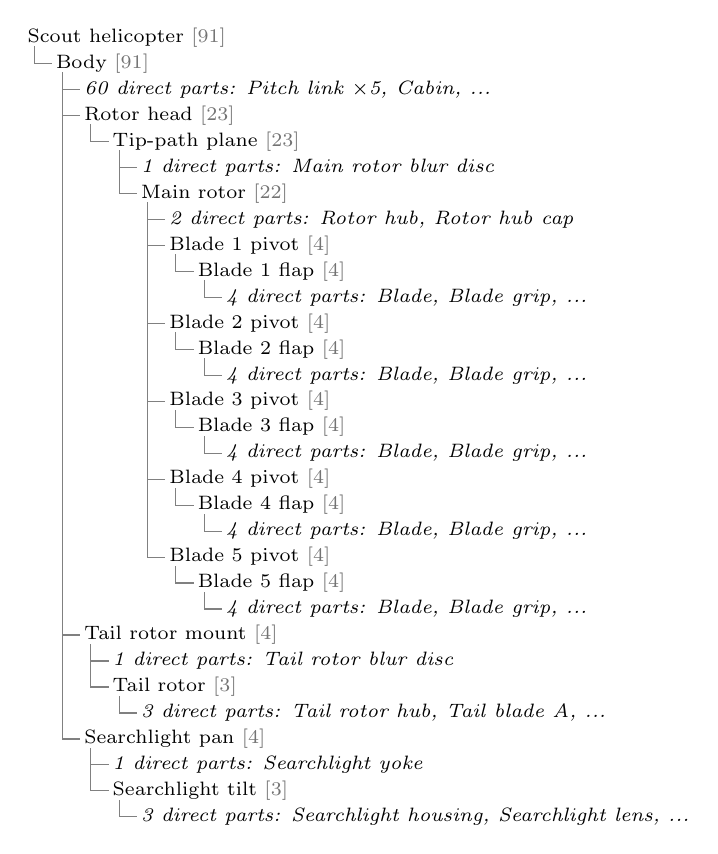
\begin{tikzpicture}[x=0.36cm,y=-0.33cm,font=\scriptsize]
\node[anchor=west,inner sep=0pt] (n0) at (0,0) {Scout helicopter \textcolor{black!55}{[91]}};
\node[anchor=west,inner sep=0pt] (n1) at (1,1) {Body \textcolor{black!55}{[91]}};
\draw[black!50,thin] (0.25,0.35) |- (0.88,1);
\node[anchor=west,inner sep=0pt] (n2) at (2,2) {\textit{60 direct parts: Pitch link $\times$5, Cabin, ...}};
\draw[black!50,thin] (1.25,1.35) |- (1.88,2);
\node[anchor=west,inner sep=0pt] (n3) at (2,3) {Rotor head \textcolor{black!55}{[23]}};
\draw[black!50,thin] (1.25,1.35) |- (1.88,3);
\node[anchor=west,inner sep=0pt] (n4) at (3,4) {Tip-path plane \textcolor{black!55}{[23]}};
\draw[black!50,thin] (2.25,3.35) |- (2.88,4);
\node[anchor=west,inner sep=0pt] (n5) at (4,5) {\textit{1 direct parts: Main rotor blur disc}};
\draw[black!50,thin] (3.25,4.35) |- (3.88,5);
\node[anchor=west,inner sep=0pt] (n6) at (4,6) {Main rotor \textcolor{black!55}{[22]}};
\draw[black!50,thin] (3.25,4.35) |- (3.88,6);
\node[anchor=west,inner sep=0pt] (n7) at (5,7) {\textit{2 direct parts: Rotor hub, Rotor hub cap}};
\draw[black!50,thin] (4.25,6.35) |- (4.88,7);
\node[anchor=west,inner sep=0pt] (n8) at (5,8) {Blade 1 pivot \textcolor{black!55}{[4]}};
\draw[black!50,thin] (4.25,6.35) |- (4.88,8);
\node[anchor=west,inner sep=0pt] (n9) at (6,9) {Blade 1 flap \textcolor{black!55}{[4]}};
\draw[black!50,thin] (5.25,8.35) |- (5.88,9);
\node[anchor=west,inner sep=0pt] (n10) at (7,10) {\textit{4 direct parts: Blade, Blade grip, ...}};
\draw[black!50,thin] (6.25,9.35) |- (6.88,10);
\node[anchor=west,inner sep=0pt] (n11) at (5,11) {Blade 2 pivot \textcolor{black!55}{[4]}};
\draw[black!50,thin] (4.25,6.35) |- (4.88,11);
\node[anchor=west,inner sep=0pt] (n12) at (6,12) {Blade 2 flap \textcolor{black!55}{[4]}};
\draw[black!50,thin] (5.25,11.35) |- (5.88,12);
\node[anchor=west,inner sep=0pt] (n13) at (7,13) {\textit{4 direct parts: Blade, Blade grip, ...}};
\draw[black!50,thin] (6.25,12.35) |- (6.88,13);
\node[anchor=west,inner sep=0pt] (n14) at (5,14) {Blade 3 pivot \textcolor{black!55}{[4]}};
\draw[black!50,thin] (4.25,6.35) |- (4.88,14);
\node[anchor=west,inner sep=0pt] (n15) at (6,15) {Blade 3 flap \textcolor{black!55}{[4]}};
\draw[black!50,thin] (5.25,14.35) |- (5.88,15);
\node[anchor=west,inner sep=0pt] (n16) at (7,16) {\textit{4 direct parts: Blade, Blade grip, ...}};
\draw[black!50,thin] (6.25,15.35) |- (6.88,16);
\node[anchor=west,inner sep=0pt] (n17) at (5,17) {Blade 4 pivot \textcolor{black!55}{[4]}};
\draw[black!50,thin] (4.25,6.35) |- (4.88,17);
\node[anchor=west,inner sep=0pt] (n18) at (6,18) {Blade 4 flap \textcolor{black!55}{[4]}};
\draw[black!50,thin] (5.25,17.35) |- (5.88,18);
\node[anchor=west,inner sep=0pt] (n19) at (7,19) {\textit{4 direct parts: Blade, Blade grip, ...}};
\draw[black!50,thin] (6.25,18.35) |- (6.88,19);
\node[anchor=west,inner sep=0pt] (n20) at (5,20) {Blade 5 pivot \textcolor{black!55}{[4]}};
\draw[black!50,thin] (4.25,6.35) |- (4.88,20);
\node[anchor=west,inner sep=0pt] (n21) at (6,21) {Blade 5 flap \textcolor{black!55}{[4]}};
\draw[black!50,thin] (5.25,20.35) |- (5.88,21);
\node[anchor=west,inner sep=0pt] (n22) at (7,22) {\textit{4 direct parts: Blade, Blade grip, ...}};
\draw[black!50,thin] (6.25,21.35) |- (6.88,22);
\node[anchor=west,inner sep=0pt] (n23) at (2,23) {Tail rotor mount \textcolor{black!55}{[4]}};
\draw[black!50,thin] (1.25,1.35) |- (1.88,23);
\node[anchor=west,inner sep=0pt] (n24) at (3,24) {\textit{1 direct parts: Tail rotor blur disc}};
\draw[black!50,thin] (2.25,23.35) |- (2.88,24);
\node[anchor=west,inner sep=0pt] (n25) at (3,25) {Tail rotor \textcolor{black!55}{[3]}};
\draw[black!50,thin] (2.25,23.35) |- (2.88,25);
\node[anchor=west,inner sep=0pt] (n26) at (4,26) {\textit{3 direct parts: Tail rotor hub, Tail blade A, ...}};
\draw[black!50,thin] (3.25,25.35) |- (3.88,26);
\node[anchor=west,inner sep=0pt] (n27) at (2,27) {Searchlight pan \textcolor{black!55}{[4]}};
\draw[black!50,thin] (1.25,1.35) |- (1.88,27);
\node[anchor=west,inner sep=0pt] (n28) at (3,28) {\textit{1 direct parts: Searchlight yoke}};
\draw[black!50,thin] (2.25,27.35) |- (2.88,28);
\node[anchor=west,inner sep=0pt] (n29) at (3,29) {Searchlight tilt \textcolor{black!55}{[3]}};
\draw[black!50,thin] (2.25,27.35) |- (2.88,29);
\node[anchor=west,inner sep=0pt] (n30) at (4,30) {\textit{3 direct parts: Searchlight housing, Searchlight lens, ...}};
\draw[black!50,thin] (3.25,29.35) |- (3.88,30);
\end{tikzpicture}
\end{minipage}\hfill
\begin{minipage}[t]{0.42\linewidth}\vspace{0pt}% generated by report/gen_tables.py from build/scene_export.json -- do not edit
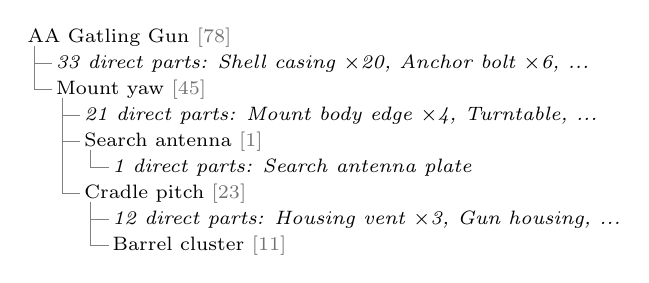
\begin{tikzpicture}[x=0.36cm,y=-0.33cm,font=\scriptsize]
\node[anchor=west,inner sep=0pt] (n0) at (0,0) {AA Gatling Gun \textcolor{black!55}{[78]}};
\node[anchor=west,inner sep=0pt] (n1) at (1,1) {\textit{33 direct parts: Shell casing $\times$20, Anchor bolt $\times$6, ...}};
\draw[black!50,thin] (0.25,0.35) |- (0.88,1);
\node[anchor=west,inner sep=0pt] (n2) at (1,2) {Mount yaw \textcolor{black!55}{[45]}};
\draw[black!50,thin] (0.25,0.35) |- (0.88,2);
\node[anchor=west,inner sep=0pt] (n3) at (2,3) {\textit{21 direct parts: Mount body edge $\times$4, Turntable, ...}};
\draw[black!50,thin] (1.25,2.35) |- (1.88,3);
\node[anchor=west,inner sep=0pt] (n4) at (2,4) {Search antenna \textcolor{black!55}{[1]}};
\draw[black!50,thin] (1.25,2.35) |- (1.88,4);
\node[anchor=west,inner sep=0pt] (n5) at (3,5) {\textit{1 direct parts: Search antenna plate}};
\draw[black!50,thin] (2.25,4.35) |- (2.88,5);
\node[anchor=west,inner sep=0pt] (n6) at (2,6) {Cradle pitch \textcolor{black!55}{[23]}};
\draw[black!50,thin] (1.25,2.35) |- (1.88,6);
\node[anchor=west,inner sep=0pt] (n7) at (3,7) {\textit{12 direct parts: Housing vent $\times$3, Gun housing, ...}};
\draw[black!50,thin] (2.25,6.35) |- (2.88,7);
\node[anchor=west,inner sep=0pt] (n8) at (3,8) {Barrel cluster \textcolor{black!55}{[11]}};
\draw[black!50,thin] (2.25,6.35) |- (2.88,8);
\end{tikzpicture}
\\[3mm]% generated by report/gen_tables.py from build/scene_export.json -- do not edit
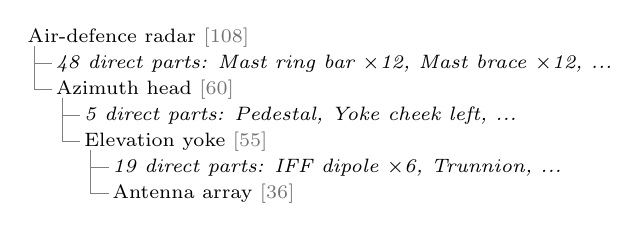
\begin{tikzpicture}[x=0.36cm,y=-0.33cm,font=\scriptsize]
\node[anchor=west,inner sep=0pt] (n0) at (0,0) {Air-defence radar \textcolor{black!55}{[108]}};
\node[anchor=west,inner sep=0pt] (n1) at (1,1) {\textit{48 direct parts: Mast ring bar $\times$12, Mast brace $\times$12, ...}};
\draw[black!50,thin] (0.25,0.35) |- (0.88,1);
\node[anchor=west,inner sep=0pt] (n2) at (1,2) {Azimuth head \textcolor{black!55}{[60]}};
\draw[black!50,thin] (0.25,0.35) |- (0.88,2);
\node[anchor=west,inner sep=0pt] (n3) at (2,3) {\textit{5 direct parts: Pedestal, Yoke cheek left, ...}};
\draw[black!50,thin] (1.25,2.35) |- (1.88,3);
\node[anchor=west,inner sep=0pt] (n4) at (2,4) {Elevation yoke \textcolor{black!55}{[55]}};
\draw[black!50,thin] (1.25,2.35) |- (1.88,4);
\node[anchor=west,inner sep=0pt] (n5) at (3,5) {\textit{19 direct parts: IFF dipole $\times$6, Trunnion, ...}};
\draw[black!50,thin] (2.25,4.35) |- (2.88,5);
\node[anchor=west,inner sep=0pt] (n6) at (3,6) {Antenna array \textcolor{black!55}{[36]}};
\draw[black!50,thin] (2.25,4.35) |- (2.88,6);
\end{tikzpicture}
\end{minipage}
\caption{Hierarchies of the helicopter (left; the tip-path-plane node tilts with the cyclic and each blade flaps and feathers under its own \emph{Blade $i$ flap} node), the AA gun and
the radar (right), from the export. Captures of the same machines are in Fig.~\ref{fig:machines}.}
\label{fig:tree-air}
\end{figure}

% ---------------------------------------------------------------------
\subsection{Gate barrier, windsock and flag}
\sheetfig{s03_gate}
\sheetfig{s03_flag}
Three animated base objects: the possessable \emph{boom barrier} (\partsBarrier{} parts, five red and five white stripes, counterweight, lamps), the \emph{windsock} (\partsWindsock{} parts: pole, swivel, five chained
segments) and the \emph{flag} (\partsFlag{} parts: a flag of 12 chained strips). Windsock and flag share one wind function.

\begin{figure}[h]
\centering
\begin{minipage}[t]{0.32\linewidth}\vspace{0pt}% generated by report/gen_tables.py from build/scene_export.json -- do not edit
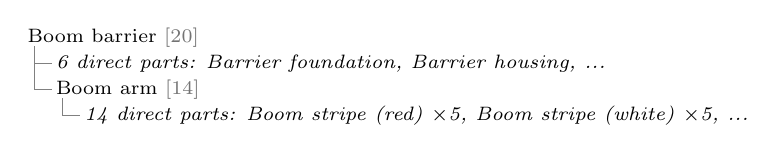
\begin{tikzpicture}[x=0.36cm,y=-0.33cm,font=\scriptsize]
\node[anchor=west,inner sep=0pt] (n0) at (0,0) {Boom barrier \textcolor{black!55}{[20]}};
\node[anchor=west,inner sep=0pt] (n1) at (1,1) {\textit{6 direct parts: Barrier foundation, Barrier housing, ...}};
\draw[black!50,thin] (0.25,0.35) |- (0.88,1);
\node[anchor=west,inner sep=0pt] (n2) at (1,2) {Boom arm \textcolor{black!55}{[14]}};
\draw[black!50,thin] (0.25,0.35) |- (0.88,2);
\node[anchor=west,inner sep=0pt] (n3) at (2,3) {\textit{14 direct parts: Boom stripe (red) $\times$5, Boom stripe (white) $\times$5, ...}};
\draw[black!50,thin] (1.25,2.35) |- (1.88,3);
\end{tikzpicture}
\end{minipage}\hfill
\begin{minipage}[t]{0.32\linewidth}\vspace{0pt}% generated by report/gen_tables.py from build/scene_export.json -- do not edit
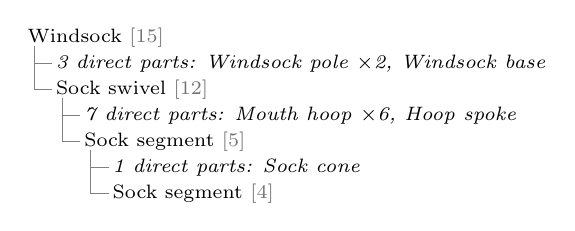
\begin{tikzpicture}[x=0.36cm,y=-0.33cm,font=\scriptsize]
\node[anchor=west,inner sep=0pt] (n0) at (0,0) {Windsock \textcolor{black!55}{[15]}};
\node[anchor=west,inner sep=0pt] (n1) at (1,1) {\textit{3 direct parts: Windsock pole $\times$2, Windsock base}};
\draw[black!50,thin] (0.25,0.35) |- (0.88,1);
\node[anchor=west,inner sep=0pt] (n2) at (1,2) {Sock swivel \textcolor{black!55}{[12]}};
\draw[black!50,thin] (0.25,0.35) |- (0.88,2);
\node[anchor=west,inner sep=0pt] (n3) at (2,3) {\textit{7 direct parts: Mouth hoop $\times$6, Hoop spoke}};
\draw[black!50,thin] (1.25,2.35) |- (1.88,3);
\node[anchor=west,inner sep=0pt] (n4) at (2,4) {Sock segment \textcolor{black!55}{[5]}};
\draw[black!50,thin] (1.25,2.35) |- (1.88,4);
\node[anchor=west,inner sep=0pt] (n5) at (3,5) {\textit{1 direct parts: Sock cone}};
\draw[black!50,thin] (2.25,4.35) |- (2.88,5);
\node[anchor=west,inner sep=0pt] (n6) at (3,6) {Sock segment \textcolor{black!55}{[4]}};
\draw[black!50,thin] (2.25,4.35) |- (2.88,6);
\end{tikzpicture}
\end{minipage}\hfill
\begin{minipage}[t]{0.32\linewidth}\vspace{0pt}% generated by report/gen_tables.py from build/scene_export.json -- do not edit
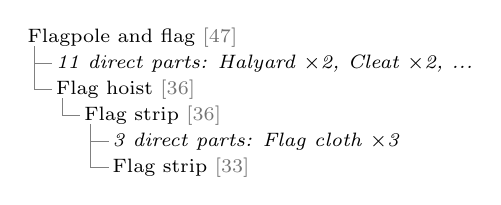
\begin{tikzpicture}[x=0.36cm,y=-0.33cm,font=\scriptsize]
\node[anchor=west,inner sep=0pt] (n0) at (0,0) {Flagpole and flag \textcolor{black!55}{[47]}};
\node[anchor=west,inner sep=0pt] (n1) at (1,1) {\textit{11 direct parts: Halyard $\times$2, Cleat $\times$2, ...}};
\draw[black!50,thin] (0.25,0.35) |- (0.88,1);
\node[anchor=west,inner sep=0pt] (n2) at (1,2) {Flag hoist \textcolor{black!55}{[36]}};
\draw[black!50,thin] (0.25,0.35) |- (0.88,2);
\node[anchor=west,inner sep=0pt] (n3) at (2,3) {Flag strip \textcolor{black!55}{[36]}};
\draw[black!50,thin] (1.25,2.35) |- (1.88,3);
\node[anchor=west,inner sep=0pt] (n4) at (3,4) {\textit{3 direct parts: Flag cloth $\times$3}};
\draw[black!50,thin] (2.25,3.35) |- (2.88,4);
\node[anchor=west,inner sep=0pt] (n5) at (3,5) {Flag strip \textcolor{black!55}{[33]}};
\draw[black!50,thin] (2.25,3.35) |- (2.88,5);
\end{tikzpicture}
\end{minipage}
\caption{Hierarchies of the boom barrier, the windsock and the flag (export). The windsock and the flag are chains in
which every segment is the child of the previous one.}
\end{figure}

% ---------------------------------------------------------------------
\subsection{Environment, terrain and backdrop}
The Gouraud environment (\partsEnv{} parts) holds the compound's fence, watchtower, sandbag walls, tent, supply caches, radio mast,
spruces of cone whorls, broadleaf trees of sphere clumps, bushes, boulders and military dressing (HESCO blocks, jersey chicane, fighting position). The trench strip and the bunker
footprint are cleared of vegetation (T78). The terrain (130 rings $\times$ 384 slices, 49\,921
vertices, 97\,440 triangles, trench hole; T13/T61) has a levelled bunker pad,
a creek, a track, a berm and a mound over the bunker roof (T60). The backdrop (\partsBackdrop{} parts:
hills, a 46-pine tree line, a far radio tower at 100\,m) starts beyond the mesh (T79: nearest part 38.0\,m).

\begin{figure}[h]
\centering
\begin{minipage}[t]{0.6\linewidth}\vspace{0pt}% generated by report/gen_tables.py from build/scene_export.json -- do not edit
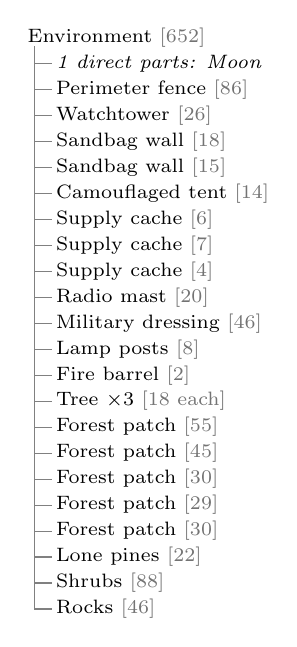
\begin{tikzpicture}[x=0.36cm,y=-0.33cm,font=\scriptsize]
\node[anchor=west,inner sep=0pt] (n0) at (0,0) {Environment \textcolor{black!55}{[652]}};
\node[anchor=west,inner sep=0pt] (n1) at (1,1) {\textit{1 direct parts: Moon}};
\draw[black!50,thin] (0.25,0.35) |- (0.88,1);
\node[anchor=west,inner sep=0pt] (n2) at (1,2) {Perimeter fence \textcolor{black!55}{[86]}};
\draw[black!50,thin] (0.25,0.35) |- (0.88,2);
\node[anchor=west,inner sep=0pt] (n3) at (1,3) {Watchtower \textcolor{black!55}{[26]}};
\draw[black!50,thin] (0.25,0.35) |- (0.88,3);
\node[anchor=west,inner sep=0pt] (n4) at (1,4) {Sandbag wall \textcolor{black!55}{[18]}};
\draw[black!50,thin] (0.25,0.35) |- (0.88,4);
\node[anchor=west,inner sep=0pt] (n5) at (1,5) {Sandbag wall \textcolor{black!55}{[15]}};
\draw[black!50,thin] (0.25,0.35) |- (0.88,5);
\node[anchor=west,inner sep=0pt] (n6) at (1,6) {Camouflaged tent \textcolor{black!55}{[14]}};
\draw[black!50,thin] (0.25,0.35) |- (0.88,6);
\node[anchor=west,inner sep=0pt] (n7) at (1,7) {Supply cache \textcolor{black!55}{[6]}};
\draw[black!50,thin] (0.25,0.35) |- (0.88,7);
\node[anchor=west,inner sep=0pt] (n8) at (1,8) {Supply cache \textcolor{black!55}{[7]}};
\draw[black!50,thin] (0.25,0.35) |- (0.88,8);
\node[anchor=west,inner sep=0pt] (n9) at (1,9) {Supply cache \textcolor{black!55}{[4]}};
\draw[black!50,thin] (0.25,0.35) |- (0.88,9);
\node[anchor=west,inner sep=0pt] (n10) at (1,10) {Radio mast \textcolor{black!55}{[20]}};
\draw[black!50,thin] (0.25,0.35) |- (0.88,10);
\node[anchor=west,inner sep=0pt] (n11) at (1,11) {Military dressing \textcolor{black!55}{[46]}};
\draw[black!50,thin] (0.25,0.35) |- (0.88,11);
\node[anchor=west,inner sep=0pt] (n12) at (1,12) {Lamp posts \textcolor{black!55}{[8]}};
\draw[black!50,thin] (0.25,0.35) |- (0.88,12);
\node[anchor=west,inner sep=0pt] (n13) at (1,13) {Fire barrel \textcolor{black!55}{[2]}};
\draw[black!50,thin] (0.25,0.35) |- (0.88,13);
\node[anchor=west,inner sep=0pt] (n14) at (1,14) {Tree $\times$3 \textcolor{black!55}{[18 each]}};
\draw[black!50,thin] (0.25,0.35) |- (0.88,14);
\node[anchor=west,inner sep=0pt] (n15) at (1,15) {Forest patch \textcolor{black!55}{[55]}};
\draw[black!50,thin] (0.25,0.35) |- (0.88,15);
\node[anchor=west,inner sep=0pt] (n16) at (1,16) {Forest patch \textcolor{black!55}{[45]}};
\draw[black!50,thin] (0.25,0.35) |- (0.88,16);
\node[anchor=west,inner sep=0pt] (n17) at (1,17) {Forest patch \textcolor{black!55}{[30]}};
\draw[black!50,thin] (0.25,0.35) |- (0.88,17);
\node[anchor=west,inner sep=0pt] (n18) at (1,18) {Forest patch \textcolor{black!55}{[29]}};
\draw[black!50,thin] (0.25,0.35) |- (0.88,18);
\node[anchor=west,inner sep=0pt] (n19) at (1,19) {Forest patch \textcolor{black!55}{[30]}};
\draw[black!50,thin] (0.25,0.35) |- (0.88,19);
\node[anchor=west,inner sep=0pt] (n20) at (1,20) {Lone pines \textcolor{black!55}{[22]}};
\draw[black!50,thin] (0.25,0.35) |- (0.88,20);
\node[anchor=west,inner sep=0pt] (n21) at (1,21) {Shrubs \textcolor{black!55}{[88]}};
\draw[black!50,thin] (0.25,0.35) |- (0.88,21);
\node[anchor=west,inner sep=0pt] (n22) at (1,22) {Rocks \textcolor{black!55}{[46]}};
\draw[black!50,thin] (0.25,0.35) |- (0.88,22);
\end{tikzpicture}
\end{minipage}\hfill
\begin{minipage}[t]{0.36\linewidth}\vspace{0pt}\footnotesize
\begin{tabular}{@{}ll@{}}\toprule
Terrain mesh & 130 $\times$ 384, $r=36$\,m\\
Creek depth & $-0.41$\,m (T42)\\
Berm & $+0.44$\,m (T42)\\
Apron level & $-0.30$\,m\\
Far ground top & $-0.35$\,m (T43)\\\bottomrule
\end{tabular}
\end{minipage}
\caption{Environment groups (export, depth 1) and terrain values measured by T42/T43.}
\end{figure}

% =====================================================================
\section{From Object to Pixel: View, Projection, Clipping, Rasterisation, Depth}\label{sec:geomchain}
\pipestrip{3}
A vertex has left its object ($\vect p_\text{world}=W\,\vect p_\text{local}$, Chapters~\ref{sec:builder}--\ref{sec:transform}). This chapter follows it until it is a pixel with a depth:
\begin{equation}
\vect p_\text{clip}=P\,V\,W\,\vect p_\text{local},\qquad \vect p_\text{ndc}=\frac{\vect p_\text{clip}}{w_\text{clip}},\qquad
\begin{pmatrix}x_s\\y_s\\z_s\end{pmatrix}=\begin{pmatrix}(x_\text{ndc}+1)\,W_s/2\\(y_\text{ndc}+1)\,H_s/2\\(z_\text{ndc}+1)/2\end{pmatrix}.
\end{equation}
\emph{Reading: world, then camera frame, then squashed by the lens into a cube, divided by depth, stretched onto the screen.}

\subsection{View matrix: lookAt}
The camera sits at $\vect e$ looking at $\vect c$ with up $\vect u_0$. Its frame is $\vect f=\mathrm{normalize}(\vect c-\vect e)$, $\vect s=\mathrm{normalize}(\vect f\times\vect u_0)$, $\vect u=\vect s\times\vect f$ (right, true up, forward), and the view matrix expresses world points in it:
\begin{equation}
V=\begin{pmatrix}s_x&s_y&s_z&-\vect s\!\cdot\!\vect e\\u_x&u_y&u_z&-\vect u\!\cdot\!\vect e\\-f_x&-f_y&-f_z&\vect f\!\cdot\!\vect e\\0&0&0&1\end{pmatrix}.
\end{equation}
\emph{Reading: translate the eye to the origin, then rotate so that the camera looks down $-z$.} (\code{lookAt}, Listing~\ref{lst:LookAt}.)
\lstLookAt

\subsection{Projection matrix: perspective}
With vertical field of view $\theta$, aspect ratio $a$ and near and far planes $n,f$, and $t=1/\tan(\theta/2)$:
\begin{equation}
P=\begin{pmatrix}t/a&0&0&0\\0&t&0&0\\0&0&-\dfrac{f+n}{f-n}&-\dfrac{2fn}{f-n}\\0&0&-1&0\end{pmatrix}.
\end{equation}
\emph{Reading: $x$ and $y$ are scaled by the focal length; the last row copies $-z_\text{view}$ into $w$, so the later division by $w$ makes distant things smaller.} Depth is non-linear: for $d=-z_\text{view}$,
$z_\text{ndc}=\dfrac{f+n}{f-n}-\dfrac{2fn}{(f-n)\,d}$, so $d=n\mapsto-1$ and $d=f\mapsto+1$; most of the range is spent near the camera, so the depth view linearises it, $z_\text{lin}=2nf/(f+n-z_\text{ndc}(f-n))$. The orthographic matrix of the moon's shadow cascades has no division: $2/(r-l)$, $2/(t-b)$, $-2/(f-n)$ on the diagonal plus a translation column.
\lstPerspective
\paragraph{Worked example.} Take $\theta=60^\circ$ ($t=1.7321$), $a=16/9$, $n=0.1$, $f=200$ and a point at view-space $(1,\,0.5,\,-10)$. Then $x_c=1.7321/1.7778\cdot1=0.9743$, $y_c=1.7321\cdot0.5=0.8660$,
$z_c=\frac{200.1}{199.9}\cdot10-\frac{40}{199.9}=9.810$, $w_c=10$. Dividing by $w_c$: $\vect p_\text{ndc}=(0.0974,\,0.0866,\,0.9810)$, inside $[-1,1]^3$, so it is visible. On a $1920\times1080$ viewport the pixel is $x_s=(0.0974+1)\cdot960=1053.5$,
$y_s=(0.0866+1)\cdot540=586.8$, window depth $z_s=0.9905$.

\subsection{Clipping, NDC and the viewport}
In clip space a point is inside if $-w\le x,y,z\le w$; the hardware clips triangles against these six planes \emph{before} the division (avoiding $w\le0$). Afterwards the visible volume is the cube $[-1,1]^3$ (NDC), and the viewport transform maps it to pixels. The program also culls whole parts: a part's bounding sphere
$r=\tfrac12\sqrt{s_x^2+s_y^2+s_z^2}$ is tested against the six planes of $PV$ (Gribb--Hartmann: plane $=\text{row}_4\pm\text{row}_{1,2,3}$).

\subsection{Back-face culling and rasterisation}
After projection the signed area $\tfrac12[(x_1-x_0)(y_2-y_0)-(x_2-x_0)(y_1-y_0)]$ is positive for front faces; negative ones are discarded (\code{GL\_CCW}, \code{GL\_BACK}). The \emph{rasteriser} then finds the pixels whose centres lie inside the triangle with edge functions
$E_{01}(\vect p)=(x_1-x_0)(y-y_0)-(y_1-y_0)(x-x_0)$ (inside if the three have the same sign), and the barycentric coordinates are the normalised edge functions: $\lambda_2=E_{01}(\vect p)/2A$, and so on ($A$ the triangle area). These $\lambda$ are what Chapter~\ref{sec:interp} interpolates with.
\begin{figure}[h]
\centering
\begin{subfigure}{0.49\linewidth}\picdia{raster_edges}{\linewidth}\caption{edge functions and barycentric weights}\end{subfigure}
\begin{subfigure}{0.49\linewidth}\picdia{frustum_ndc}{\linewidth}\caption{view frustum $\to$ NDC cube}\end{subfigure}
\caption{Rasterisation and the view volume.}
\end{figure}

\subsection{Depth test: the Z-buffer}
Each fragment's depth $z_s$ is compared with the stored value (\code{GL\_LESS}): if smaller, colour and depth are written, otherwise the fragment is discarded. Key \texttt{Z} switches the test off, showing the painter's-order result (e.g.\ the rover through the tree that hides it). The depth buffer is reused by the shadow maps, SSAO, fog, SSR and the vision's ground-ray hits.
\begin{figure}[h]
\centering
\piclab{buffer_03_depth}{0.7\linewidth}
\caption{The depth buffer of the current scene, linearised for display (in-program render, near = dark).}\label{fig:diag}
\end{figure}

\subsection{The workbook view of the same matrices}
The workbook rebuilds $T$, $R$, $S$ and $M=TRS$ of every part with sum-of-products cell formulas ($m_{ij}=\sum_k a_{ik}b_{kj}$) and checks them against the exported matrices: the largest difference is $8.7\times10^{-8}$ on the UAV gimbal chain and $2.4\times10^{-5}$ over the whole workbook (single-precision rounding).
\begin{figure}[h]
\centering
\picsheet{sheet_mmult}{\linewidth}
\caption{\sheetcaption{sheet_mmult}}
\end{figure}

% =====================================================================
\section{Colour Interpolation and the Three Shading Models}\label{sec:interp}
\pipestrip{5}
Flat, Gouraud and Phong shading answer one question: \emph{where in a triangle is the lighting equation evaluated, and how are the values in between obtained?}

\subsection{Barycentric interpolation}
\autofig{diagrams}{B1_barycentric}
Every pixel inside a triangle $\vect p_0,\vect p_1,\vect p_2$ has barycentric coordinates $(\lambda_0,\lambda_1,\lambda_2)$, $\lambda_i\ge0$, $\sum\lambda_i=1$. Any per-vertex quantity $a_i$ (colour, normal, light term) is blended linearly:
\begin{equation}a=\lambda_0a_0+\lambda_1a_1+\lambda_2a_2 .\end{equation}
Under perspective the hardware interpolates with the clip-space $w_i$:
\begin{equation}\lambda_i'=\frac{\lambda_i/w_i}{\sum_j\lambda_j/w_j},\qquad a=\sum_i\lambda_i'a_i,\end{equation}
so colours do not swim on slanted surfaces. Example: intensities $0.2,0.8,0.5$ with $\lambda=(0.2,0.3,0.5)$ give $0.53$.

\subsection{Flat, Gouraud and Phong in one table}
\begin{table}[h]
\centering\small
\caption{The three models as implemented (\code{ShaderSources.cpp}).}\label{tab:shademodels}
\begin{tabular}{@{}llp{4.4cm}p{4.5cm}@{}}
\toprule Model & Lighting evaluated & Interpolated across the triangle & Used for\\\midrule
Flat & once per triangle, at its centroid, with the face normal $\vect N_f$ & nothing (the \code{flat} qualifier) & the bunker and base buildings: sharp architectural facets\\
Gouraud & at every \emph{vertex} & the light terms (colours) & terrain, vegetation, props\\
Phong & at every \emph{fragment} & the normal $\vect N$ (re-normalised) & UAV, rover, tank, helicopter, AA gun, radar: moving highlights\\\bottomrule
\end{tabular}
\end{table}

\paragraph{Flat.} A geometry shader (Listing~\ref{lst:FlatGeom}) computes $\vect N_f=\mathrm{normalize}((\vect p_1-\vect p_0)\times(\vect p_2-\vect p_0))$, evaluates the light once at the centroid $(\vect p_0+\vect p_1+\vect p_2)/3$ and emits the same \code{flat} terms for all three vertices. A zero-area triangle falls back to an up normal.
\lstFlatGeom
\paragraph{Gouraud.} The vertex shader (Listing~\ref{lst:GouraudVert}) calls \code{computeLight(position, normal)} per vertex, with the normal transformed by $(M^{-1})^\top$; the light \emph{terms} are interpolated and the fragment shader multiplies them by the albedo.
\lstGouraudVert
\paragraph{Phong.} The fragment shader re-normalises the interpolated normal and calls \code{computeLight} per pixel: \code{FragColor = shadeFragment(computeLight(vWorld, N), vWorld, N)}.
All three paths end in the same \code{shadeFragment}, so shadows, occlusion, procedural surfaces, fog and thermal output are identical; \emph{only the place where the lighting equation is evaluated differs}. Keys \texttt{O}\,\texttt{F}\,\texttt{G}\,\texttt{P} force one model for the whole scene (T19).

\subsection{What the difference looks like}
\autofig{figures_lab}{shading_sphere_compare}
\autofig{diagrams}{B2_shading_models_real}
\sheetfig{s08_shading}
Gouraud can miss a highlight completely. With $(\vect N\!\cdot\!\vect H)^n$, $n=64$, a vertex whose normal is $20^\circ$ from $\vect H$ gets $\cos^{64}20^\circ\approx0.019$, while a pixel mid-triangle whose interpolated normal points at $\vect H$ gets $1.0$: per-vertex lighting sees only the dark corners, so the highlight vanishes or smears. Flat shading gives each facet a constant grey (exaggerated by \emph{Mach bands}); Gouraud removes the steps but keeps slope breaks at vertex lines. Figure~\ref{fig:shademodels} renders one object with all three models.
\begin{figure}[h]
\centering
\piclab{shading_models}{\linewidth}
\caption{The same sphere and cylinder under Flat, Gouraud and Phong shading (in-program render): facets, linear ramps with missing highlight, and a per-pixel highlight.}\label{fig:shademodels}
\end{figure}
\paragraph{Fragment-dependent factors.} Because Flat and Gouraud light before the fragment stage, shadow-map visibility, ambient occlusion and procedural relief (next chapter) are applied afterwards to the interpolated terms, which are therefore kept separate (moon, beacon, spotlight, practical lights) rather than summed.

% =====================================================================
\section{Lighting, Materials and Surface Detail}\label{sec:shading}
\pipestrip{6}
\subsection{Lambert and Blinn--Phong: diffuse and shininess}
\autofig{diagrams}{B3_lambert}
\autofig{figures_lab}{materials_blinnphong_row}
For a light with direction $\vect L$ (towards the light), normal $\vect N$, view vector $\vect V$ and halfway vector $\vect H=\mathrm{normalize}(\vect L+\vect V)$, the classic model is
\begin{equation}
I=k_d\,\max(\vect N\!\cdot\!\vect L,0)\;+\;k_s\,\max(\vect N\!\cdot\!\vect H,0)^{n}.
\end{equation}
The first term is \emph{Lambert's law}: received energy follows $\cos\theta=\vect N\!\cdot\!\vect L$, scattered evenly. The second is the highlight; the \emph{shininess} $n$ sets its width, which falls to half at $\alpha_{1/2}=\arccos 2^{-1/n}$: $9.4^\circ$ for $n=16$, $4.7^\circ$ for $n=64$, $2.4^\circ$ for $n=256$. This is the \code{uPbr==0} branch of Listing~\ref{lst:Brdf} (key \texttt{B}); \code{uSpecular} is $k_s$, \code{uShininess} is $n$.

\subsection{Cook--Torrance with GGX: roughness and metalness}
\autofig{diagrams}{C3_specular_grid}
The default model treats a surface as microscopic mirrors (\emph{microfacets}); with roughness $\rho$, $\alpha=\rho^2$ and
\begin{equation}
f_s=\frac{D(\vect H)\,G(\vect N,\vect V,\vect L)\,F(\vect V,\vect H)}{4(\vect N\!\cdot\!\vect V)(\vect N\!\cdot\!\vect L)},
\end{equation}
\begin{equation}
D=\frac{\alpha^2}{\pi\bigl((\vect N\!\cdot\!\vect H)^2(\alpha^2-1)+1\bigr)^2},\qquad
G=\prod_{x\in\{V,L\}}\frac{\vect N\!\cdot\!x}{(\vect N\!\cdot\!x)(1-k)+k},\ \ k=\frac{(\rho+1)^2}{8},\qquad
F=F_0+(1-F_0)(1-\vect V\!\cdot\!\vect H)^5 .
\end{equation}
$D$ is the GGX normal distribution (facets facing $\vect H$, with the long tail that makes highlights natural), $G$ the Smith--Schlick masking term (facets hide each other at grazing angles) and $F$ the Schlick Fresnel term (every surface mirrors at grazing angles). The base reflectivity is $F_0=\mathrm{mix}(0.04,\text{albedo},m)$ with metalness $m$: dielectrics reflect 4\,\% white, metals their own colour; the diffuse part is $(1-F)(1-m)$ times Lambert. Listing~\ref{lst:Brdf} is the whole function.
\lstBrdf
\paragraph{Shininess $\leftrightarrow$ roughness.} Materials that give only a shininess get $\rho=\mathrm{clamp}(1-\log_2(n)/8,\,0.08,\,0.95)$ (\code{pbrRoughness}, \code{Material.h}); others set roughness explicitly. Figure~\ref{fig:matgrid} shows roughness against metalness under one light.
\begin{figure}[h]
\centering
\begin{subfigure}{0.58\linewidth}\piclab{material_grid}{\linewidth}\caption{roughness (columns) $\times$ metalness (rows)}\end{subfigure}
\begin{subfigure}{0.40\linewidth}\picdia{ggx_curves}{\linewidth}\caption{$D$ for several $\rho$; Blinn--Phong lobes}\end{subfigure}
\caption{Material response. The highlight narrows and brightens as roughness falls; metals tint the highlight, dielectrics do not.}\label{fig:matgrid}
\end{figure}

\subsection{Light sources and attenuation}
\begin{itemize}
  \item \textbf{L0, moon:} directional, colour $(0.55,0.62,0.80)$, intensity 0.95.
  \item \textbf{L1, beacon:} a point light at the bunker's beacon, colour $(1,0.25,0.10)$, attenuation $1/(1+0.35\,d+0.45\,d^2)$, intensity pulsing $0.6$--$2.0$ at 1\,Hz.
  \item \textbf{L2, UAV searchlight:} a spot with smooth cone between $9^\circ$ and $14^\circ$: $c=\mathrm{clamp}\frac{\cos\gamma-\cos14^\circ}{\cos9^\circ-\cos14^\circ}$, radiance $\propto c^2/(1+0.05\,d+0.03\,d^2)$, intensity 5.
  \item \textbf{Practical lights:} any emissive part declared with \code{asLight(material, intensity, range, cone)} is also a light. The renderer ranks them by distance over range and uploads the \textbf{16} best per view (\code{gatherPracticals}). Falloff is a windowed inverse square (Listing~\ref{lst:Practical}): $f=\mathrm{saturate}(1-(d/R)^4)^2/(1+d^2)$, exactly 0 at the range $R$ (no popping), optionally cut by a spot cone.
  \item \textbf{Dynamic explosion lights:} flashes, burning wrecks and muzzle flashes join the same list and rank ahead of lamps (score halved).
\end{itemize}
\lstPractical
\begin{figure}[h]
\centering
\picdia{attenuation}{0.7\linewidth}
\caption{Attenuation curves of the beacon, the searchlight and a practical lamp (computed from the constants above).}
\end{figure}

\begin{figure}[h]
\centering
\picsheet{sheet_lighting}{\linewidth}
\caption{\sheetcaption{sheet_lighting}}
\end{figure}
\subsection{Shadows: cascades and PCF}
\sheetfig{s07_attenuation}
\sheetfig{s07_charts}
The moon casts shadows with two orthographic cascades in a depth-texture array. The \emph{near cascade} covers the view-frustum slice from the near plane to a split distance (10--14\,m by preset) and follows the camera; the \emph{world cascade} covers a 39\,m sphere around the base, never moves, and is snapped to whole texels so edges do not shimmer (T34). Its static casters are rendered once into a cache; only \code{dynamic} nodes (vehicles, UAVs, debris) are redrawn each frame. The cache key is the explode value plus the foliage setting. Listing~\ref{lst:MoonShadow} blends the cascades over the last 20\,\% of the split distance. Each lookup uses a normal-offset bias and a rotated Poisson disc of 8 (HIGH) or 16 (ULTRA/EPIC) hardware-PCF taps; the fraction of lit taps gives a soft penumbra. The searchlight has its own perspective shadow map along its axis.
\lstMoonShadow
\begin{figure}[h]
\centering
\piclab{shadow_cascades}{0.8\linewidth}
\caption{Moon shadow cascades (colour = cascade).}
\end{figure}

\subsection{Ambient light, indoor mask, thermal heat}
Ambient is a sky/ground hemisphere. The bunker must receive no sky or moonlight: \code{WalkSpace} supplies up to eight indoor boxes and Listing~\ref{lst:Indoor} computes a smooth mask. Inside it ambient is multiplied by $0.012$, moon, beacon and searchlight by $1-\text{mask}$, fog by $1-0.85\,\text{mask}$, and practical lights carry an \emph{inside} flag so a tunnel lamp does not light the surface above.
\lstIndoor
The thermal view reuses the shader with apparent temperature $h=h_0+0.04\min(E,1.5)$ (intrinsic heat plus a little capped absorbed light), minus $0.05$ times the wetness on passive surfaces.

\subsection{Procedural albedo patterns}
There are no image textures. The \code{Surface} enum selects a pattern evaluated from world position with value, fractal ($\mathrm{fbm}$) or cellular noise: concrete, paint chips, bark, lichen, leaves, and the set of Table~\ref{tab:surfaces}. Patterns are triplanar: coordinates are $(x,z)$ on up-facing surfaces and $(z,y)$ or $(x,y)$ on side faces by dominant normal axis, so a pattern continues across a scaled cube without UV unwrap.
\begin{table}[h]
\centering\small
\caption{Procedural surfaces (\code{Surface} values 12--18).}\label{tab:surfaces}
\begin{tabular}{@{}rllp{8.4cm}@{}}
\toprule Id & Name & Used on & Pattern\\\midrule
12 & Corrugated & containers, huts, radar shelter & ribs every 7.6\,cm along world $Y$, dirt runs, rust at the bottom\\
13 & Hesco & HESCO bastion walls & welded wire grid (7.6\,cm) over sand-bag bulges\\
14 & Hazard & bunker door portal, barriers, signs & yellow/black $45^\circ$ stripes with wear\\
15 & Screen & bunker consoles, control panel & dark phosphor, grid, rotating sweep, blips, text bars (emissive)\\
16 & Asphalt & the gate road & aggregate speckle, cracks, polished wheel lanes\\
17 & Camo & tank, helicopter, AA gun, nets & three-blob woodland camouflage\\
18 & SteelPlate & blast doors, armour, radar door & 0.6\,m panels, seam lines, rivet rows, worn edges\\\bottomrule
\end{tabular}
\end{table}
\begin{figure}[h]
\centering
\piclab{surface_patterns}{\linewidth}
\caption{The procedural surfaces on flat boxes (in-program render): concrete, corrugated, HESCO, hazard, screen, asphalt, camo, steel plate.}
\end{figure}

\subsection{Surface relief: procedural bump}
\code{surfaceHeight(q)} in \code{ShaderSources.cpp} gives each procedural material a height field in the same triplanar coordinates as its albedo (concrete pores 1.5\,mm, bark ridges, rock, planks, corrugated ribs 9\,mm, HESCO mesh and bags, asphalt
aggregate, camo paint chips, steel seams $-3$\,mm and rivets $+2$\,mm). Listing~\ref{lst:Bump} shows \code{surfaceBump(P,N)}, which takes central differences $\partial h/\partial u,\partial h/\partial v$ ($\epsilon=4$\,mm) and tilts the normal,
$\vect N_b=\mathrm{normalize}\bigl(\vect N-(h_u\vect T+h_v\vect B)\,k\bigr)$, where $\vect T,\vect B$ is the tangent frame of the dominant face and $k$ fades out from 12 to 40\,m (no far shimmer). Because the Gouraud and Flat paths evaluate lighting before the fragment
stage, the light terms are \emph{re-aimed} by the Lambert ratio
\begin{equation}
k_L=\mathrm{clamp}\!\left(\frac{\max(\vect N_b\!\cdot\!\vect L,0)+0.03}{\max(\vect N\!\cdot\!\vect L,0)+0.03},\,0.3,\,2\right),
\end{equation}
applied to the moon and searchlight diffuse terms ($k_L$) and specular terms ($k_L^2$); a cavity factor $\mathrm{clamp}(0.6+0.4\,\vect N_b\!\cdot\!\vect N+0.5(N_{b,y}-N_y),0.6,1.15)$ darkens pits that face away from the sky, and the bumped normal also feeds the SSR surface buffer. The bump is active
only in HDR on HIGH and above (\code{uGroundDetail}); screens, foliage and the ground have their own code. \lstBump
\begin{figure}[h]
\centering
\piclab{bump_on_off}{\linewidth}
\caption{Bump off (left) and on (right) for corrugated metal, HESCO and steel plate: ribs, mesh and rivets catch the light (in-program render).}
\end{figure}
The planned \emph{reflection probe} (a low-resolution sky cubemap for metal and glass) is \textbf{not} implemented; reflections still come from SSR and the analytic sky.


% =====================================================================
\section{Reflection and the Post Chain}\label{sec:reflection}
\pipestrip{8}
A rasteriser has no ray tracing, so reflection is faked from what is already on screen; no image or cube map is used.

\subsection{Specular ambient and wet surfaces}
\autofig{diagrams}{D2_fresnel_reflectivity}
Every shaded point adds a specular \emph{ambient} term $t_{sa}$ from the sky colour (modulated by ambient occlusion), so smooth metal shows a faint sky reflection even in the dark. Rain adds a water film on up-facing surfaces:
$\text{film}=w\cdot\mathrm{clamp}(1.4\,N_y+0.1,0,1)$ with the wetness $w\in[0,1]$; wet porous materials (concrete, wood, soil, HESCO, asphalt) darken by up to 45\,\%, roughness drops towards 0.3, and the ground shader mirrors the practical lights with a
per-fragment GGX highlight. The reflectivity stored for the next pass is $\max(0.45\,\text{film},\;m\,(1-\rho)^2\,0.6)$: wet ground and polished metal reflect, rough paint does not.

\subsection{Screen-space reflection (SSR)}
The main pass writes a second render target with the world normal and that reflectivity. A later pass (Listing~\ref{lst:Ssr}, key \texttt{F7}) reconstructs the world position $\vect P$ of each reflective pixel from depth, reflects the view direction, $\vect R=\mathrm{reflect}(\vect V,\vect N)$, and \emph{marches} $\vect Q(t)=\vect P+t\vect R$:
\begin{enumerate}
  \item \textbf{Ray march.} Start at $t=0.04(1+\text{jitter})$ (per-pixel jitter that TAA averages out) and grow the step, $t\leftarrow1.09\,t+0.03$, for 48 steps (64 on EPIC). Each sample is projected to the screen, $\vect q=\tfrac12\,\text{clip}_{xy}/\text{clip}_w+\tfrac12$;
  leaving the screen or going behind the camera ends the march.
  \item \textbf{Hit test.} The sample's linear depth (the clip $w$) is compared with the depth buffer at $\vect q$; a hit is a ray behind the surface by less than $0.15+0.04\,t+0.01\,d_0$ ($d_0$ = distance of $\vect P$ from the camera), growing with distance so far gaps are not missed.
  \item \textbf{Bisection.} Six bisection steps between the last miss $t_a$ and the hit $t_b$ find the crossing and remove stair-stepping.
  \item \textbf{Weights.} The fetched colour is multiplied by an \emph{edge fade} (smoothstep over 7\,\% of each border), a \emph{distance fade}, and the Fresnel factor
  $F=0.02+0.98(1-\vect N\!\cdot\!(-\vect V))^5$ mixed as $\mathrm{mix}(0.35,1,F)$.
\end{enumerate}
\lstSsr
\begin{figure}[h]
\centering
\piclab{ssr_on_off}{\linewidth}
\caption{Screen-space reflection off (left) and on (right) on wet ground: lamp posts and vehicles appear in the puddles (in-program render, key \texttt{F7}).}
\end{figure}
\begin{figure}[h]
\centering
\begin{subfigure}{0.48\linewidth}\picdia{ssr_raymarch}{\linewidth}\caption{ray march and bisection}\end{subfigure}
\begin{subfigure}{0.48\linewidth}\picdia{fresnel}{\linewidth}\caption{Schlick Fresnel vs.\ angle}\end{subfigure}
\caption{The geometry of the SSR march and the Fresnel weight.}
\end{figure}
Limits: SSR reflects only what is on screen, and reflections on rough surfaces are not blurred; there is no environment probe.

\subsection{The post chain in brief}
The linear HDR scene then passes through the chain of Chapter~\ref{sec:pipeline}: TAA, bloom, auto-exposure and \textbf{tone mapping} with the fitted ACES curve of Listing~\ref{lst:Aces}, $\mathrm{ACES}(x)=\frac{x(2.51x+0.03)}{x(2.43x+0.59)+0.14}$, followed by the sRGB transfer, vignette and grain.
\lstAces
\begin{figure}[h]
\centering
\piclab{pipeline_buffers}{\linewidth}
\caption{Intermediate buffers of one frame (in-program render): depth, normal, ambient occlusion, fog, HDR scene, bloom, final.}
\end{figure}

% =====================================================================
\section{Rendering Pipeline}\label{sec:pipeline}
\pipestrip{8}
The frame is rendered in linear light into a multisampled HDR target and post-processed. The passes in
Fig.~\ref{fig:frame} match the GPU timer labels in \code{Renderer.cpp}/\code{RendererFrame.cpp}: \emph{uav camera (CV), shadow maps, pre-pass, ssao, volumetric fog, scene,
combine + ssr, taa, exposure / agc, lens flare, depth of field, resolve, bloom, composite}. This chapter is a pass-by-pass overview; shadows,
lighting, SSR and tone mapping are explained once, in Chapters~\ref{sec:shading} and~\ref{sec:reflection}.

\begin{figure}[h]
\centering
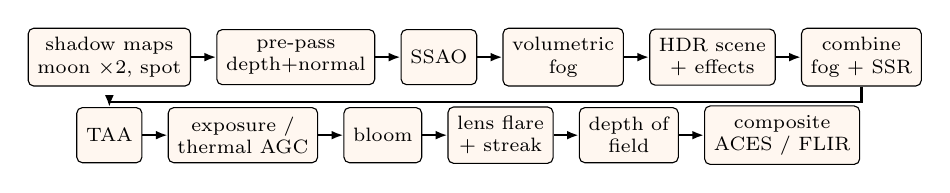
\begin{tikzpicture}[node distance=2.6mm and 3.2mm, every node/.style={font=\scriptsize},
  box/.style={draw,rounded corners=2pt,minimum height=7mm,align=center,fill=orange!6},
  arr/.style={-{Latex[length=1.5mm]},thick}]
  \node[box] (s) {shadow maps\\moon $\times2$, spot};
  \node[box,right=of s] (p) {pre-pass\\depth+normal};
  \node[box,right=of p] (a) {SSAO};
  \node[box,right=of a] (f) {volumetric\\fog};
  \node[box,right=of f] (m) {HDR scene\\+ effects};
  \node[box,right=of m] (c) {combine\\fog + SSR};
  \node[box,below=of s] (t) {TAA};
  \node[box,right=of t] (e) {exposure /\\thermal AGC};
  \node[box,right=of e] (b) {bloom};
  \node[box,right=of b] (l) {lens flare\\+ streak};
  \node[box,right=of l] (d) {depth of\\field};
  \node[box,right=of d] (o) {composite\\ACES / FLIR};
  \foreach \x/\y in {s/p,p/a,a/f,f/m,m/c,t/e,e/b,b/l,l/d,d/o} \draw[arr] (\x)--(\y);
  \draw[arr] (c.south) -- ++(0,-2mm) -| (t.north);
\end{tikzpicture}
\caption{The frame. A separate raw heat render from the gimbal camera ($320\times240$, no post-processing) feeds the
thermal tracker.}
\label{fig:frame}
\end{figure}

\subsection{Shadows}
\autofig{diagrams}{G1_render_pipeline}
Two moon cascades and a spot map are rendered first; cascade fitting, the static cache, snapping and PCF are described in Chapter~\ref{sec:shading}.
The world cascade covers a sphere of radius $r=\texttt{kBaseRadius}+3=39$\,m, i.e.\ $2r/4096=1.9$\,cm per texel on EPIC and 3.8\,cm at 2048.
The cascade centre is snapped in light space, $c'=\lfloor c/\Delta\rfloor\Delta$, $\Delta=2r/\text{res}$ (T34). A node is dynamic if \code{SceneNode::dynamic} is set
(the Scene marks the UAVs, the rovers and every controllable object other than a drone controller's own root).

\subsection{SSAO, volumetric fog, bloom}
\textbf{SSAO} samples a normal-oriented hemisphere (8 samples HIGH, 16 EPIC) around each pixel of the depth/normal
pre-pass (half resolution, full resolution on EPIC) and is blurred depth-aware. \textbf{Volumetric fog} ray-marches a
height fog $\sigma(y)=\sigma_0e^{-0.22y}$ lit by the moon, the beacon and the practical lights with single
scattering, $L\mathrel{+}=T\,L_\text{in}(1-e^{-\sigma\Delta s})$, $T\mathrel{*}=e^{-\sigma\Delta s}$ (24 steps HIGH, 48
ULTRA, 64 EPIC at half resolution). The searchlight shaft is a thin cone that a coarse march would miss, so the ray is
intersected analytically with the cone $(\vect d\cdot\vect a)^2=\cos^2\gamma\,|\vect x-\vect s|^2$ and only that
interval is sampled, using the spot shadow map. \textbf{Bloom} uses a soft-knee threshold, a 13-tap downsample chain and a tent upsample.

\subsection{TAA, SSR, DOF, motion blur, flare, auto-exposure, tone mapping}
\begin{itemize}
  \item \textbf{TAA}: Halton jitter, reprojection from the full-resolution depth, Catmull--Rom history, YCoCg variance
  clipping, cut detection; captures accumulate 8 frames. Switch: \texttt{F6}.
  \item \textbf{SSR}: reflections on wet ground from the surface buffer (Section~\ref{sec:reflection}). Switch: \texttt{F7}.
  \item \textbf{Lens flare}: ghosts, halo and an anamorphic streak from the bloom chain; off indoors. Switch: \texttt{F8}.
  \item \textbf{Auto-exposure}: log-average luminance, adapted over time, clamped to $\pm1.5$\,EV around $\log_2 L=-5.2$ so night stays dark. Switch: \texttt{F9}; \texttt{+}/\texttt{-} adjust manually.
  \item \textbf{Depth of field}: golden-angle bokeh gather (\texttt{F10}); \textbf{motion blur}: from depth reprojection (cinematic shots and video).
  \item \textbf{ACES}: the curve of Listing~\ref{lst:Aces} (Chapter~\ref{sec:reflection}), sRGB, scotopic (Purkinje) shift and split toning, vignette and grain.
\end{itemize}

\subsection{Thermal sensor model}
In THERMAL view (key \texttt{V}; \texttt{Y} switches between the gimbal and external view) heat is
rendered as a scalar and the sensor pass applies: automatic gain control from the frame's heat range, digital detail enhancement against a wide local mean, a palette (\texttt{T}: ironbow, white-hot, rainbow,
black-hot), temporal noise, fixed-pattern column/row offsets, dead pixels, a narcissus vignette, heat shimmer above
hot parts and a periodic NUC shutter freeze (\texttt{Q} forces one). The zoom (mouse wheel) is WFOV/MFOV/NFOV at
40/20/8$^\circ$. The FLIR-style HUD shows compass, gimbal scales, telemetry and the target box with slant range and track state.
Explosion particles and scorch marks write a heat value too, so a fireball is a bright blob and a wreck stays hot while it cools.

\subsection{Effects renderer}
Explosions and weapons are drawn by \code{EffectsRenderer} (\code{rendering/Effects.cpp}) as instanced
quads (the lab's unit cube, only its $+Z$ face used), one instance being $4\times$\code{vec4}. All kinds share one program and one premultiplied-alpha blend state
\code{glBlendFunc(ONE, ONE\_MINUS\_SRC\_ALPHA)}: smoke writes (lit colour$\cdot\alpha$, $\alpha$), emissive sprites write
(HDR colour, $\sim0$), so ``additive'' and ``alpha'' differ only in the alpha value. Smoke, trail and
dust are drawn sorted back to front, then the emissive group (fire, flash, sparks, embers, tracers, shock waves), also sorted, because
the fire's soot edge needs the order. Scorch decals and projectile bodies are drawn after the solids with the
depth test. The eight particle types are listed in Table~\ref{tab:fx}; the particle cap is 4\,000 (T104), and low-priority smoke, trail and
dust are dropped first.

\begin{table}[h]
\centering\small
\caption{Effect particle types (\code{EffectType}, \code{EffectsData.h}) and their role. Brightness is scaled at spawn in
\code{Combat::spawn} (flash $\times0.12$, fire $\times0.14$, spark and ember $\times0.45$) to land at a few HDR units under the
night exposure.}
\label{tab:fx}
\begin{tabular}{@{}rllp{9.3cm}@{}}
\toprule
Id & Type & Blend & Role\\\midrule
0 & Fire & emissive & fireball puff, orange $\to$ red $\to$ dark, soot edge\\
1 & Smoke & lit, alpha & grows, dark grey (explosion) or light grey (exhaust)\\
2 & Spark & emissive & tiny hot streak along its velocity\\
3 & Flash & emissive & very short bright sphere (detonation, muzzle flash)\\
4 & Shockwave & emissive & expanding faint ring on the ground\\
5 & Trail & lit, alpha & thin missile and shell exhaust puff\\
6 & Dust & lit, alpha & brown dust kicked by blasts, tracks, rotor wash\\
7 & Ember & emissive & glowing debris speck that falls and cools\\\bottomrule
\end{tabular}
\end{table}

\subsection{Quality presets}
\sheetfig{s09_pipeline_passes}
\sheetfig{s09_features}
\begin{table}[h]
\centering\small
\caption{Presets from \code{qualityProfile()} (RendererFrame.cpp); EPIC is auto-selected on NVIDIA / discrete GPUs
(override with \cli{quality}). Values not listed keep the HIGH defaults.}
\label{tab:presets}
\begin{tabular}{@{}lrrrrrrrr@{}}
\toprule
Preset & MSAA & Moon / spot map & SSAO & PCF & Fog steps & Grass blades & Rain drops & Fireflies\\\midrule
LOW & 2 & 1024 / off & off & 8 & off & 14\,000 & 6\,000 & 60\\
HIGH & 4 & 2048 / 1024 & 8 & 8 & 24 & 35\,000 & 14\,000 & 200\\
ULTRA & 8 & 4096 / 2048 & 16 & 16 & 48 & 140\,000 & 36\,000 & 400\\
EPIC & 4 + TAA & 4096 / 2048 & 16, full res & 16 & 64 & 450\,000 & 60\,000 & 700\\\bottomrule
\end{tabular}
\end{table}
Also: SSR, DOF and motion blur are on for ULTRA and EPIC; TAA on for HIGH and above; foliage density 0.2 / 0.5 / 0.7 / 1.0.

% =====================================================================
\section{Rover Intelligence: MicroMouse and Line Following}\label{sec:rover}
\pipestrip{10}
The intruder rover is a differential-drive robot split as in a MicroMouse / line-follower competition: a grid \emph{planner} and a \emph{controller} that follows the planned line with five infrared sensors (both in \code{ai/HideController.cpp}).

\subsection{The grid}
\autofig{diagrams}{E1_planner_grids}
The compound is $80\times80$ cells of 0.5\,m over $[-20,20]^2$. A cell is \emph{free} if vertical segments through the robot's body (centre plus eight points on its radius, up to 0.8\,m) miss every static part, with a 0.30\,m planning margin. A cell is \emph{hidden} from an observer (a UAV) if segments from five body points to it are blocked by an occluder. The test maps the segment into the primitive's unit space with $W^{-1}$, so spheres, cones and cylinders are intersected exactly (T25, T31, T37), and a 2\,m bucket grid makes it fast (T44: identical to brute force over 516 occluders).

\subsection{Flood fill: BFS for hiding}
When hiding, the goals are the hidden cells; the \emph{flood fill} is a breadth-first search over the 4-neighbourhood that stores in each free cell its step count $D$ to the nearest goal, the wave a MicroMouse spreads from the maze centre (Listing~\ref{lst:Flood}). Preferred goals are hidden cells whose free neighbours are all hidden (deep shadow); otherwise any hidden cell.
\lstFlood
\begin{figure}[h]
\centering
\begin{subfigure}{0.49\linewidth}\picdia{flood_bfs}{\linewidth}\caption{BFS distance field to the hidden cells}\end{subfigure}
\begin{subfigure}{0.49\linewidth}\picdia{flood_dijkstra}{\linewidth}\caption{Weighted field to the objective}\end{subfigure}
\caption{The two distance fields on the real compound grid (from the program's data). Dark = near the goal; white cells are blocked.}\label{fig:flood}
\end{figure}

\subsection{Weighted flood fill: Dijkstra for infiltration}
\autofig{diagrams}{E2_flood_dijkstra}
When infiltrating, the rover has an \emph{objective} (a camp asset). Dijkstra's algorithm with a priority queue computes the field from the objective cell; stepping into a cell costs, in $1/16$ units,
\begin{equation}c(\text{cell})=16+24\,[\text{exposed}]+\lfloor24\,n(\text{cell})\rfloor,\end{equation}
where \emph{exposed} means some UAV can see the cell and $n\in[0,1)$ is a value-noise field seeded per rover. A step costs one cell-length, plus 1.5 if exposed, plus up to 1.5 of random preference: rovers favour shadow and each picks different corridors (the ``random paths'' of T144) yet reaches the objective (T143). Exposure is recomputed at each replan (every 1.6\,s).
\lstDijkstra

\subsection{Steepest descent and Chaikin smoothing}
The path is read off the field by \emph{steepest descent}: step to the smallest neighbour until a goal is reached, keeping the current heading among equals so the route has few turns (Listing~\ref{lst:Descend}). The staircase of cell centres is rounded by Chaikin's corner cutting: every segment $\vect a\vect b$ is replaced by the points at $\tfrac14$ and $\tfrac34$ of its length, $\vect q=\tfrac34\vect a+\tfrac14\vect b$, $\vect r=\tfrac14\vect a+\tfrac34\vect b$, three times (Listing~\ref{lst:Chaikin}), converging to a quadratic B-spline. The line starts under the robot along its heading.
\lstDescend
\lstChaikin
\begin{figure}[h]
\centering
\picdia{path_chaikin}{0.8\linewidth}
\caption{A staircase route (cell centres) and its Chaikin-smoothed virtual line (real route from the planner).}
\end{figure}

\subsection{Line follower: IR sensors, PD steering, differential drive}
The planned line is \emph{virtual}, 10\,cm wide. Five IR sensors at lateral offsets $x_i=-0.12+0.06\,i$ m sit 0.31\,m ahead of the robot centre; sensor $i$ is \emph{active} if within 5\,cm of the line. The normalised error from the mean active offset is
\begin{equation}e=\frac{1}{0.12}\cdot\frac{\sum_{i\in\text{active}}x_i}{|\text{active}|}\in[-1,1].\end{equation}
A PD controller gives the angular velocity, $\omega=K_pe+K_d\,\dot e$ with $K_p=3.2$, $K_d=0.25$ (clamped to $\pm2.5$\,rad/s), and speed falls with error, $v=v_\text{max}(1-0.6|e|)$, $v_\text{max}=0.75$\,m/s. The differential drive converts $(v,\omega)$ to track speeds
$v_{L,R}=v\mp\omega W/2$ ($W=0.5$\,m), limited to 2\,m/s$^2$ wheel acceleration, and integrates $v=\tfrac12(v_L+v_R)$, $\dot\psi=(v_R-v_L)/W$. With no sensor on the line the robot sweeps towards the line's side and replans after 0.8\,s; if blocked it pivots and, after 1.2\,s, reverses.
\lstFollowLine
\begin{figure}[h]
\centering
\begin{subfigure}{0.49\linewidth}\picdia{ir_sensors}{\linewidth}\caption{sensor bar on the line: error $e$ vs.\ pattern}\end{subfigure}
\begin{subfigure}{0.49\linewidth}\picdia{rover_trace}{\linewidth}\caption{a driven path against the planned line}\end{subfigure}
\caption{The line follower. Left: the five sensors and the resulting error; right: a rover's actual trace over its virtual line.}
\end{figure}

\subsection{Behaviours and tests}
\emph{Hide}: goals are hidden cells, BFS field. \emph{Infiltrate}: goal is the objective, Dijkstra field, route committed for 1.6\,s. \emph{Evade}: a UAV within 5\,m switches the rover to hiding for 4\,s, then it resumes. Tests: T27 (BFS field valid, descent reaches a goal: start value 8, 8 cells), T28 (the rover drives into the UAV's blind spot within 60\,s), T143--T145 (infiltration, random routes ending 4.32\,m apart after 25\,s, evasion).

% =====================================================================
\section{Computer Vision: How a UAV Sees the Rovers}\label{sec:vision}
\pipestrip{9}
Each UAV carries a thermal camera on its gimbal. The autonomy never reads a rover's position: everything it knows comes from a $320\times240$ image of apparent temperature. Figure~\ref{fig:cvoverview} follows one frame to a confirmed, fused, predicted track.
\begin{figure}[h]
\centering
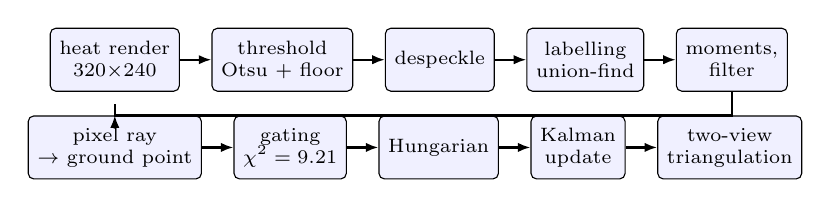
\begin{tikzpicture}[node distance=3mm and 4mm, every node/.style={font=\scriptsize},
  box/.style={draw,rounded corners=2pt,minimum height=8mm,align=center,fill=blue!6},arr/.style={-{Latex[length=1.6mm]},thick}]
  \node[box] (a) {heat render\\$320{\times}240$};
  \node[box,right=of a] (b) {threshold\\Otsu + floor};
  \node[box,right=of b] (c) {despeckle};
  \node[box,right=of c] (d) {labelling\\union-find};
  \node[box,right=of d] (e) {moments,\\filter};
  \node[box,below=of a] (f) {pixel ray\\$\to$ ground point};
  \node[box,right=of f] (g) {gating\\$\chi^2=9.21$};
  \node[box,right=of g] (h) {Hungarian};
  \node[box,right=of h] (i) {Kalman\\update};
  \node[box,right=of i] (j) {two-view\\triangulation};
  \foreach \x/\y in {a/b,b/c,c/d,d/e,f/g,g/h,h/i,i/j} \draw[arr] (\x)--(\y);
  \draw[arr] (e.south) -- ++(0,-3mm) -| (f.north);
\end{tikzpicture}
\caption{The vision chain, per UAV frame (top) and shared by the squad (bottom).}\label{fig:cvoverview}
\end{figure}

\subsection{The thermal image}
\autofig{diagrams}{G2_cv_pipeline}
The scene is drawn again from the gimbal pose into a $320\times240$ target ($40^\circ$ vertical field of view) with the \emph{raw heat} output instead of colour. Each material has an intrinsic temperature $h_0$ (ground $0.15$, bunker $0.34$, a rover's motor box $0.97$, a charred wreck $0.95$ cooling
as $0.3+0.65e^{-t/40\,\text{s}}$) plus a little absorbed light and ground noise; the result is read back as 8-bit values (heat $\times255$). Rovers are the only ground-level parts hotter than $0.9$; static props stay below the blob threshold (T41: hottest prop $0.74$), as do tyre footprints ($\le0.51$) and the wreck.
\begin{figure}[h]
\centering
\begin{subfigure}{0.49\linewidth}\piclab{cv_thermal}{\linewidth}\caption{raw heat image (UAV 0)}\end{subfigure}
\begin{subfigure}{0.49\linewidth}\piclab{cv_threshold}{\linewidth}\caption{after Otsu + floor threshold}\end{subfigure}\\[1mm]
\begin{subfigure}{0.49\linewidth}\piclab{cv_despeckle}{\linewidth}\caption{after despeckle}\end{subfigure}
\begin{subfigure}{0.49\linewidth}\piclab{cv_labels}{\linewidth}\caption{labelled blobs, centroids, orientation}\end{subfigure}
\caption{The image stage on a real frame, one picture per step.}\label{fig:cvstages}
\end{figure}

\subsection{Threshold: Otsu and a fixed floor}
\autofig{diagrams}{F1_threshold_histogram}
Otsu's method picks the level $t$ that splits the 256-bin histogram into a dark and a bright class by maximising the between-class variance
$\sigma_b^2(t)=\omega_0(t)\,\omega_1(t)\,[\mu_0(t)-\mu_1(t)]^2$ ($\omega$ class probabilities, $\mu$ class means). The threshold is $\max(204,\ t_\text{Otsu}+1)$: the floor (heat 0.80) stops a dark frame from producing targets,
Otsu raises the level in warm clutter (T132: bimodal image, $t=40$).
\lstOtsu

\subsection{Despeckle}
A hot pixel with fewer than two hot 8-neighbours is removed: single-pixel noise disappears, real blobs survive (T130: 396 speckle pixels removed, three discs kept).
\lstDespeckle

\subsection{Connected components: two-pass union-find}
\autofig{diagrams}{F3_union_find}
The \emph{first pass} scans row by row; a hot pixel takes the smallest root among its labelled 8-neighbours (W, NW, N, NE) or a new label, and
\emph{records those labels as equivalent} in a union-find forest (path compression; the larger root points to the smaller). The \emph{second pass} replaces each label by its root and renumbers $1..n$. A U-shaped blob whose arms got different labels is merged (T131).
\lstLabel

\subsection{Blob features: moments, orientation, elongation}
\autofig{diagrams}{F4_blob_moments}
One pass accumulates $n,\sum x,\sum y,\sum x^2,\sum y^2,\sum xy$ per component. The centroid is $(\bar x,\bar y)=(\sum x/n,\sum y/n)$ and the second central moments
$\mu_{20}=\frac{\sum x^2}{n}-\bar x^2$, $\mu_{02}=\frac{\sum y^2}{n}-\bar y^2$, $\mu_{11}=\frac{\sum xy}{n}-\bar x\bar y$ form the covariance matrix $C=\begin{bmatrix}\mu_{20}&\mu_{11}\\\mu_{11}&\mu_{02}\end{bmatrix}$ whose eigenvalues are
\begin{equation}\lambda_{1,2}=\frac{\mu_{20}+\mu_{02}}{2}\pm\sqrt{\Bigl(\frac{\mu_{20}-\mu_{02}}{2}\Bigr)^2+\mu_{11}^2}.\end{equation}
The \emph{orientation} of the major axis is $\tfrac12\operatorname{atan2}(2\mu_{11},\mu_{20}-\mu_{02})$ and the \emph{elongation} is $\sqrt{\lambda_1/\lambda_2}$ ($\lambda_2$ is floored at $1/12$, the variance of a single pixel). A blob is a target if its area is 2--2500 pixels (bigger is a fire), it contains a pixel $\ge230$ (an engine) and, from 6 pixels up, its elongation is at most 6 (thin streaks are tracers). T132 checks a bar: orientation $0^\circ$, elongation 10.3. The normalised coordinates
$u=2(\bar x+0.5)/320-1$, $v=1-2(\bar y+0.5)/240$ go to the geometry step; Listing~\ref{lst:Detect} is the whole image stage.
\lstDetect

\subsection{From pixel to ground point}
\sheetfig{s18_params_footprint}
The camera looks along the pitch node's $+Z$. A pixel $(u,v)$ defines the ray direction $\vect d=\mathrm{normalize}\bigl(W_\text{cam}\,(-u\,t_x,\ v\,t_y,\ 1)^\top\bigr)$ with $t_y=\tan(20^\circ)$, $t_x=t_y\cdot320/240$ (image right is local $-X$). The ground point
is where the ray meets the terrain, found by marching in 5\,cm steps until $y\le h(x,z)+h_b$ (Listing~\ref{lst:RayGround}). $h_b=0.2$\,m (\code{kSquadBlobHeight}) is the height of the rover's hot body; stopping at the ground itself would put a single-view fix about 0.27\,m beyond the rover. The standard deviation grows with range, $\sigma=0.12+0.015\,r$\,m.
\lstRayGround

\subsection{Kalman filter: one track per rover}
Each track holds $\vect x=(x,z,v_x,v_z)^\top$ and a $4\times4$ covariance $P$. The prediction over $\Delta t$ uses a constant-velocity model with white-noise acceleration of standard deviation $\sigma_a=1.5$\,m/s$^2$:
\begin{equation}
\vect x^-=F\vect x,\quad P^-=FPF^\top+Q,\quad F=\begin{bmatrix}I_2&\Delta t\,I_2\\0&I_2\end{bmatrix},\quad
Q=\sigma_a^2\begin{bmatrix}\tfrac{\Delta t^4}{4}I_2&\tfrac{\Delta t^3}{2}I_2\\\tfrac{\Delta t^3}{2}I_2&\Delta t^2I_2\end{bmatrix}.
\end{equation}
Only the position is measured: $H=[I_2\ 0]$, $R=\sigma^2I_2$. The update is
\begin{equation}
\vect y=\vect z-H\vect x^-,\quad S=HP^-H^\top+R,\quad K=P^-H^\top S^{-1},\quad \vect x=\vect x^-+K\vect y,\quad P=(I-KH)P^-.
\end{equation}
$S$ is $2\times2$ and inverted in closed form. A new track starts at the measurement with position variance $\sigma^2$ and velocity variance $4\,\text{m}^2/\text{s}^2$. T135: position error below 0.25\,m (late maximum 0.164\,m) and velocity 0.96\,m/s for a
1.2\,m/s target; the estimated velocity lets the squad aim ahead (Chapter~\ref{sec:squad}).
\lstPredict
\lstKalman
\begin{figure}[h]
\centering
\begin{subfigure}{0.49\linewidth}\picdia{kalman_demo}{\linewidth}\caption{noisy measurements, filtered track, velocity}\end{subfigure}
\begin{subfigure}{0.49\linewidth}\picdia{gating_ellipse}{\linewidth}\caption{gating ellipse and measurements}\end{subfigure}
\caption{The Kalman tracker: raw ground points (dots), filtered track (line), $\chi^2$ gate (ellipse).}
\end{figure}

\subsection{Data association: Mahalanobis gating and the Hungarian algorithm}
A measurement $\vect z$ may belong to a track only if the squared Mahalanobis distance of its innovation, $d^2=\vect y^\top S^{-1}\vect y$, is below $\chi^2_{2,0.99}=9.21$ (two degrees of freedom; 99\,\% of true measurements pass). The gate scales with the track's uncertainty (the ellipse above). For each sensor the gated costs $d^2$ form a track-by-measurement matrix and the \textbf{Hungarian algorithm}
(Kuhn--Munkres, $O(n^3)$, padded square) finds the one-to-one assignment of minimum total cost, so two nearby blobs cannot claim one track (T133: optimal in 50 of 50 random matrices against brute force over 120 permutations).
\lstMahal
\lstHungarian

\subsection{Two-view triangulation}
When both UAVs measure the same track in the same frame, the pixel rays $\vect o_1+s\vect d_1$ and $\vect o_2+t\vect d_2$ are combined. Skew lines rarely intersect, so the point is the midpoint of closest approach: minimising $|\vect o_1+s\vect d_1-\vect o_2-t\vect d_2|^2$ with
$\vect w=\vect o_1-\vect o_2$, $a=\vect d_1\!\cdot\!\vect d_1$, $b=\vect d_1\!\cdot\!\vect d_2$, $c=\vect d_2\!\cdot\!\vect d_2$, $d=\vect d_1\!\cdot\!\vect w$, $e=\vect d_2\!\cdot\!\vect w$ gives the $2\times2$ system
\begin{equation}
\begin{bmatrix}a&-b\\b&-c\end{bmatrix}\begin{bmatrix}s\\t\end{bmatrix}=\begin{bmatrix}-d\\-e\end{bmatrix}
\ \Rightarrow\ s=\frac{be-cd}{ac-b^2},\quad t=\frac{ae-bd}{ac-b^2},
\end{equation}
and $\vect p=\tfrac12(\vect o_1+s\vect d_1+\vect o_2+t\vect d_2)$ with the \emph{residual} $|\vect p_1-\vect p_2|$ as a quality measure. Parallel rays ($ac-b^2\approx0$) and points behind a camera ($s$ or $t<0$) are rejected.
The fused measurement has $\sigma=\max(0.08,\,0.5\min(\sigma_1,\sigma_2)+0.25\,\text{residual})$, tighter than a single ray (T134: 0.051\,m against 0.071\,m); orthogonal rays give the best geometry, hence the wing UAV's $90^\circ$ offset.
\lstTriangulate
\begin{figure}[h]
\centering
\picdia{triangulation}{0.75\linewidth}
\caption{Two rays from two UAVs, their closest points, the midpoint and the residual; the ground-ray estimate for comparison.}
\end{figure}

\begin{figure}[h]
\centering
\picsheet{sheet_cv}{\linewidth}
\caption{\sheetcaption{sheet_cv}}
\end{figure}
\subsection{Track life cycle and merging}
\autofig{figures_lab}{cv_strip}
\sheetfig{s18_tests}
An unmatched measurement starts a \emph{tentative} track; after 3 hits it is \emph{confirmed}; with no update for 0.25\,s it \emph{coasts} (it keeps predicting; the HUD shows it amber with a ``?'') and is deleted after 3\,s. A tentative track that misses 2 frames is deleted at once (T136). Two tracks closer than 1\,m with velocities within 1\,m/s are one target: the younger merges into the older, which keeps its id (the squad's lock is on that id). A tentative younger track is fused into the older as one more Kalman measurement, so the converged velocity survives; a confirmed one hands over its whole state. Ids are never reused.
\begin{figure}[h]
\centering
\begin{subfigure}{0.49\linewidth}\piclab{cv_tracks}{\linewidth}\caption{tracks over the thermal image of UAV 0}\end{subfigure}
\begin{subfigure}{0.49\linewidth}\picfive{thermal_fpv_tracks}{\linewidth}\caption{game capture with all track boxes}\end{subfigure}
\caption{Tracks as the player sees them: boxes with ids, range and ``2-VIEW'' when triangulated.}
\end{figure}

% =====================================================================
\section{Critique and Design Goals (``Night Watch'')}\label{sec:v5plan}
\pipestrip{10}
The brief was a playable base-defence game: rovers that arrive in waves on random MicroMouse and line-follower routes, \emph{two} UAVs that patrol, track with computer vision and strike together, game feedback with sound,
and a base that looks like a hidden army camp. An enemy rover is armoured and needs four to five hits. Table~\ref{tab:crit} lists what the earlier single-UAV program lacked and where the report treats the fix; the design principles are \emph{game first}, \emph{real CV}, \emph{visible coordination} and a \emph{hidden-camp look} instead of more lamps.

\begin{table}[h]
\centering\small
\caption{Problems of the earlier program, the fix and where it is described.}\label{tab:crit}
\begin{tabular}{@{}p{6.4cm}p{6.6cm}p{2.8cm}@{}}
\toprule Problem & Fix & Section\\\midrule
Rovers only hide; fixed count, fixed spawns; deterministic descent paths & waves, random spawns and objectives, noisy-cost Dijkstra, armour (100 HP) & \ref{sec:squad}\\
One UAV, no coordination; no lead or time-on-target & two-UAV squad, roles, line-of-fire check, synchronised strike & \ref{sec:squad}\\
One thresholded blob per frame, no filter, no ids; single-ray position & Otsu, union-find, Kalman, gating, Hungarian, two-view triangulation & \ref{sec:vision}\\
No score, integrity or game markers; no sound & mission rules, HUD markers and banners, procedural audio & \ref{sec:squad}, \ref{sec:v5media}\\
Base lit like a car park; no launchers; vehicles in the open & light discipline, nets, revetments, SAM, MLRS, parked tanks & \ref{sec:v5media}\\
Flat surfaces (albedo only); reflections only in puddles & procedural bump (done); reflection probe (not implemented) & \ref{sec:v5results}\\
\texttt{Scene} as a god object & \code{Mission}, \code{Squad}, \code{CvPipeline}, \code{MultiTracker}, \code{AudioEngine} split out & \ref{sec:squad}\\\bottomrule
\end{tabular}
\end{table}
The report quotes only what the program printed: the unit tests and one headless run (Section~\ref{sec:v5results}).

\paragraph{Version 6: a day, a garrison and a real sensor.} The v5 game still had three weaknesses: it was always night, the camp was empty, and the vision saw a perfect image (plus capture-only scripted strikes). Table~\ref{tab:critsix} lists the v6 answers. Two constraints held throughout: the library defaults reproduce v5 exactly (night preset, seed 0, no garrison), so no earlier test changed, and every new number is exported for the report and the workbook.
\begin{table}[h]
\centering\small
\caption{v5 gaps, the v6 change and where it is described.}\label{tab:critsix}
\begin{tabular}{@{}p{5.6cm}p{7.6cm}p{2.6cm}@{}}
\toprule Gap in v5 & v6 change & Section\\\midrule
Permanent night, fixed lights & solar position, Kasten--Young sun, log-space preset blend, clouds and cloud shadows, solar loading below the CV floor, SKY clock & \ref{sec:daycycle}\\
An empty camp & \nSoldiers{} soldiers: spline routes from A* and string pulling, gait by FK + IK, duty roster with shifts & \ref{sec:soldiers}\\
Same intruders every run & ring spawns, via sectors, personalities, objective switch, dawn withdrawal, one seed with derived streams & \ref{sec:randompaths}\\
Ideal heat image; scripted strikes & sensor model with NUC, jitter and drops; person class; kills only through vision & \ref{sec:realcv}\\
Verification on llvmpipe only & RTX\,4070 captures, night regression, deterministic traces with rule checks & \ref{sec:v6results}\\\bottomrule
\end{tabular}
\end{table}

% =====================================================================
\section{Two-UAV Squad and Mission Rules}\label{sec:squad}
\pipestrip{10}
\subsection{Squad (\code{ai/Squad})}
\autofig{diagrams}{F8_squad_state_machine}
\sheetfig{s19_roles}
\begin{itemize}
  \item \textbf{Patrol.} The UAVs fly breathing orbits (radii 5 and 8\,m at 7.5\,m height) $180^\circ$ apart, cameras sweeping outward.
  \item \textbf{Shared track picture.} Both UAVs' blobs (Section~\ref{sec:vision}) feed one \code{MultiTracker}.
  \item \textbf{Threat ranking and roles.} The confirmed track closest to a camp asset is the target. The UAV with the longer continuous lock is \textbf{lead} (distance breaks ties when lock times differ by $\le0.2$\,s), the other \textbf{wing}. The lead holds a 6.5\,m stand-off orbit at 5\,m height; the wing flies to the point $\pm90^\circ$ around the target (the nearer side), a second attack axis and a good triangulation baseline.
  \item \textbf{Line of fire.} A UAV whose segment to the target is blocked by a static solid detours around it (timer up to 8\,s).
  \item \textbf{Reacquire.} A lost target is searched for 12\,s (\code{kSquadReacquireTime}) round its last position, then patrol resumes.
  \item \textbf{Flicker-tolerant lock.} Lock time survives short dropouts (the track coasts) instead of resetting on one empty frame. A combined strike needs a lead lock $\ge0.8$\,s and a wing lock $\ge0.5$\,s; if the wing does not lock within 2.5\,s the lead strikes alone after 1.3\,s (T138--T142).
\end{itemize}

\subsection{Time-on-target}
\autofig{diagrams}{F9_time_on_target}
\sheetfig{s19_combined}
A round starts at 8\,m/s, accelerates linearly to 60\,m/s in 0.4\,s, then holds 60\,m/s: $d(t)=8t+\tfrac12\tfrac{60-8}{0.4}t^2=8t+65t^2$ for $t\le0.4$\,s, reaching $\tfrac12(8+60)\,0.4=13.6$\,m. The
proximity fuse fires 0.5\,m short, so for a UAV-to-aim distance $D$ let $d=\max(0,D-0.5)$ and
\begin{equation}
T(d)=\begin{cases}\dfrac{-8+\sqrt{64+260\,d}}{130}, & d\le13.6\ \text{m},\\[2mm] 0.4+\dfrac{d-13.6}{60}, & d>13.6\ \text{m}.\end{cases}
\end{equation}
(The quadratic is $65t^2+8t-d=0$.) The aim point is $\vect p+\vect v\,T_\text{max}$ from the Kalman velocity. For a combined strike the farther UAV launches
at once and the nearer after the \textbf{launch delay} $\Delta=T_\text{far}-T_\text{near}$, so both rounds arrive together; each homes on its own laser spot, the predicted target position at its arrival. Each UAV has a 4-round rail; a launched round is replaced after 6\,s (\code{kUavReloadTime}).

\begin{figure}[h]
\centering
\picsheet{sheet_mission}{\linewidth}
\caption{\sheetcaption{sheet_mission}}
\end{figure}
\subsection{Mission (\code{scene/Mission})}
\autofig{diagrams}{F11_mission_waves}
\sheetfig{s19_waves}
\begin{itemize}
  \item \textbf{Waves.} Wave $n$ sends $\min(2+n,6)$ rovers (\code{kMaxRovers}), one every 3.5\,s, from random points on the compound edge (seeded RNG), facing the camp; the next wave starts 6\,s after the last rover is resolved (killed or breached).
  \item \textbf{Objectives.} Each rover gets a random camp asset (one of five) as its objective.
  \item \textbf{Breach.} A rover that reaches its objective is a breach: base integrity $-10\,\%$ (\code{kBreachDamage}). At 0\,\% the base is lost and the mission restarts at wave 1.
  \item \textbf{Score.} $+100$ per kill and $+50$ more for a combined-strike kill ($+150$ total). The HUD shows wave, score, kills (combined), enemies alive and the integrity bar (T143, T180, T181).
\end{itemize}

\subsection{Armoured rovers}
\sheetfig{s19_armour}
Four to five hits make one kill. An intruder has \code{kRoverHealth}\,$=100$ hit points. A blast of power $p$ at distance $d$ inside its damage radius $R=1.6\,p$ deals
$30\,p\,\bigl(1-\tfrac12\min(d/R,1)\bigr)$ (a direct hit counts as $d=0$): a power-1 missile does 30 at the centre and 15 at the edge, so four to seven rounds (usually four direct hits $=120$) are needed. A damaged rover limps and smokes; a hit raises an \code{EnemyHit} event, shown by the HUD as a hit marker. T105 measures five hits to kill. T140 runs the full loop with synthetic vision and printed ``kills 3 (combined 2), launched 7 / 5, score 400, wave 2, breaches 0, fused updates 479''.

\subsection{Rover infiltration}
The rover's planner (\code{HideController}) is the MicroMouse planner with the 5-sensor line follower, driving to the \emph{objective} by a weighted \textbf{Dijkstra} from the objective's cell: one cell step costs $16+24\cdot[\text{exposed}]+\lfloor24\,n(x,z)\rfloor$ in fixed point, where \emph{exposed} marks cells that a UAV can see (not hidden) and $n\in[0,1)$ is a smooth value-noise field seeded per rover, so each rover
gets a different route. A rover \textbf{commits} to a route for 1.6\,s (\code{kInfiltrateReplan}) before re-planning. If a UAV comes within 5\,m
(\code{kEvadeRadius}) it hides for 4\,s (\code{kEvadeTime}), then infiltrates again (T144, T145).

% =====================================================================
\section{Sound, Game HUD and the Hidden Camp}\label{sec:v5media}
\pipestrip{10}
\subsection{Procedural audio (\code{src/audio})}
\sheetfig{s20_sounds}
\sheetfig{s20_mixer}
Like the geometry, the sound uses no files: every clip is synthesised at 48\,kHz from seeded noise, sines and state-variable filters (\code{Dsp.h}). The only third-party code is the single-header
\code{miniaudio} (device output only). \code{AudioEngine} runs live when a device exists and does nothing headless.
\begin{itemize}
  \item \textbf{Continuous sources.} UAV hum: 4 detuned rotors $\times$ 6 blade-pass harmonics ($h^{-1.3}$) at $f=105+7v$\,Hz plus band-passed noise (one source per UAV). Helicopter: 25\,Hz blade-slap train scaled by rotor
  fraction, turbine whine. Tank: 16\,Hz firing-pulse train plus track clatter while driving. Missiles and shells in flight: noise band-passes with Doppler.
  \item \textbf{One-shots.} Launch whoosh (band-pass noise, centre $350\to2750$\,Hz); explosion (6\,ms crack, boom sweeping $100\to30$\,Hz, noise body through a closing low-pass $4\,\text{kHz}\to250$\,Hz, 90\,Hz rumble tail; length $2+1.5\,p$ s; energy grows with power);
  cannon; Gatling (55 shots/s with spin-up); door motor and clunk; wave siren (650--1000\,Hz triangle sweep); breach klaxon; radio beeps for lock, confirm and kill.
  \item \textbf{Ambient bed.} Gusting wind, seven crickets (4.3--5.2\,kHz chirps), 50\,Hz generator hum.
  \item \textbf{Spatial mix.} Equal-power panning from the listener's right vector, gain $\text{ref}/\max(d,\text{ref})$, air absorption (one-pole cut-off $16\,\text{kHz}\,e^{-d/90}$), half-strength Doppler clamped to 0.9--1.1; a 24-voice pool steals the quietest
  voice; master volume then a $\tanh$ soft limiter with ceiling 0.88 ($-1.1$\,dBFS).
  \item \textbf{Offline mix for video.} \cli{record} renders the same engine offline (\code{renderOffline}) frame by frame into a WAV and muxes it into the MP4 with ffmpeg (AAC, 192\,kb/s), so the demo video has sound.
\end{itemize}
Demo mix (10\,s, two drones, lock, launch, explosion, siren): RMS $-22.0$\,dBFS, peak $-4.46$\,dBFS (no clipping). Tests T160--T169 (12 checks) pass. Levels were tuned by RMS and spectrogram only, not by ear.

\subsection{Game HUD (\code{HudMath}, \code{AppHud})}
\sheetfig{s20_hud_tests}
The HUD logic is CPU-only and tested (T170--T178): marker projection with edge arrows, bracket size by distance (10--120\,px at 900p), banner timing and the event queue. It draws (a) \emph{enemy markers}: red brackets with ``ID n  d M'', a health bar, a pulsing LOCK ring on the squad target after 0.5\,s of lock, amber diamonds at the predicted lead points while rounds are inbound, edge arrows off-screen;
(b) \emph{UAV tags} ``UAV-1 LEAD'', ``UAV-2 WING'', ``PATROL'' with lines to the target; (c) a \emph{top bar} with wave, score, kills (combined), enemies, a base-integrity bar (green to red) and the strike state
(``COMBINED STRIKE PLANNED / INBOUND''); (d) \emph{banners}: WAVE n INCOMING, ENEMY SPOTTED, COMBINED STRIKE, ``+100'' / ``+150'', a white X hit marker, BREACH $-10$\,\% with a red edge flash, BASE LOST then RESTARTING; (e) a \emph{tactical mini-map}
(180\,px, north up) with the perimeter, camp assets, UAV triangles, track dots (red confirmed, grey tentative, amber coasting), strike lines and a sweep; (f) in the thermal FPV view, boxes for all confirmed tracks (TRK / LOCK / LOST, range,
``2-VIEW'' when triangulated). The director script has 13 shots in 120\,s; the strike captures are event-driven (they wait for the hit, kill or both rounds in flight).

\subsection{Hidden camp (\code{Launchers}, \code{Base}, \code{Structures})}
\sheetfig{s03_sam}
\sheetfig{s14_sam}
\sheetfig{s03_mlrs}
\sheetfig{s14_mlrs}
\textbf{Light discipline.} Surface practical lights number 11 (sum of intensity $\times$ range 107, against 1748 for a floodlit yard); the bunker keeps its 19 lights with entrance lamps dimmed to red. Windows are blacked out and only tiny red and blue-green markers remain, so the camp reads by moonlight, explosions and the UAV searchlights.
\textbf{Camouflage.} Camo nets (sagging thin cubes with gaps), revetments (rotated cubes) and cut branches cover vehicles, launchers, the bunker entrance and bays (670 dressing parts; 297 net panels).
\textbf{Launchers.} \emph{SAM-1}: a turntable ($\pm170^\circ$ at 22\,$^\circ$/s) carrying a cradle (elevation $0$--$60^\circ$ at 14\,$^\circ$/s, trapezoid velocity profile $v=\min(v_\text{max},\sqrt{2ad})$) with 4 canisters (90 parts); one canister per \texttt{Enter}
(elevation $\ge5^\circ$), a round slides out (8 + 60\,$t$ m/s), 8\,s reload per canister. \emph{MLRS-1}: a truck with a $6\times2$ tube pod (116 parts), mount $\pm165^\circ$ at 18\,$^\circ$/s, elevation $0$--$55^\circ$, a ripple of up to 12 tubes 0.25\,s apart, 15\,s
reload. Both are possessable (\texttt{\textbackslash} stows or readies, arrows aim, \texttt{Enter} fires). \textbf{Static vehicles.} Two parked tanks (226 parts each, turret locked) in earth revetments and an ammo bunker (43 parts); 1371 parts in total in \code{makeLaunchers()}. Tests T150--T159 pass.
Known issues: the MLRS pod can poke through its net when turned sideways; controllables are marked dynamic, so the ~1000 static revetment parts are not in the static shadow cache.


% =====================================================================
\section{Controllable Objects}\label{sec:control}
The scene has \nControllables{} controllable objects, \nPossessable{} of them \emph{possessable}: nine machines, the UAV (manual flight), tank, helicopter, AA gun, radar, blast doors and gate barrier (this section) and the SAM and MLRS launchers (Section~\ref{sec:v5media}); since v6 also the \nSoldiers{} soldiers (\texttt{F3}, Section~\ref{sec:soldiers}) and the SKY clock that carries the sun (Section~\ref{sec:daycycle}). Windsock and flag animate but are not possessable. Each implements \code{Controllable} (\code{scene/Controllable.h}): every frame only the possessed object receives the sampled \code{ControlInput} (move, turn, lift, aim, fire, action) and writes the local transforms of its own node tree in \code{update()}. In walk mode \texttt{Enter} toggles a door or barrier within 3.5\,m (T128). Keys: Appendix~\ref{app:controls}.

\begin{table}[h]
\centering\footnotesize
\setlength{\tabcolsep}{3pt}
\caption{Controllable objects. DOF = independently animated degrees of freedom.}
\label{tab:ctl}
\begin{tabular}{@{}clp{1.7cm}p{5.2cm}p{5.4cm}@{}}
\toprule
Key & Object (HUD name) & Class & Degrees of freedom & Camera views\\\midrule
5 & MBT-1 TANK & \code{Tank} & position (x, z), yaw, left/right track, turret yaw, gun pitch, recoil, hull heave/pitch, 2 antennas, MG ring & chase (9\,m behind, 55$^\circ$), sight (28$^\circ$)\\
6 & MH-6 HELICOPTER & \code{Helicopter} & position (3), yaw, pitch, roll, rotor speed, 5 blades (flap, feather), tail rotor, light pan/tilt & chase / cockpit\\
7 & AA-1 GATLING & \code{AaGun} & mount yaw, cradle pitch, cluster spin, search antenna & chase / sight\\
8 & AIR-DEFENCE RADAR & \code{Radar} & azimuth, elevation tilt, mode, TX lamp & side view (13\,m away), operator view along the beam (60$^\circ$)\\
9 & BLAST DOORS & \code{BlastDoors} & two leaves (slide), beacon spinners & door camera at $(0,-0.3,9)$\\
0 & UAV-1 DRONE & \code{DroneControl} & position (3), yaw, pitch, roll, gimbal yaw/pitch, rail rounds & chase / gimbal camera (40$^\circ$)\\
-- (\texttt{[ ]}) & GATE BARRIER & \code{GateBarrier} & boom angle, lamps & near the gate\\
F3 & SOLDIER 1--8 (v6) & \code{Soldier} & position (x, z), heading, view pitch, 2 legs (hip, knee, ankle) by gait + IK, 2 arms (shoulder 3, elbow) by swing or rifle IK, spine, head, stance (stand / crouch / wave) & chase (3.2\,m behind), first person at eye height 1.62\,m (T212)\\
-- (\texttt{[ ]}) & SKY / TIME OF DAY (v6) & \code{SkyClock} & clock hour (moves the sun sphere), auto / manual, phase jump & from the camp towards the key light\\\bottomrule
\end{tabular}
\end{table}

% ---------------------------------------------------------------------
\begin{figure}[h]
\centering
\picsheet{sheet_controllables}{\linewidth}
\caption{\sheetcaption{sheet_controllables}}
\end{figure}
\subsection{Tank: arc-length track links, skid steer, stabilised turret}
\sheetfig{s14_tank}
\paragraph{Track-link arc-length parameterisation.} The closed track path is a stadium in the hull's $(z,y)$ plane around the
sprocket ($z=-2.8$) and the idler ($z=2.8$), centre height 0.55\,m, radius $R=0.5$\,m, with perimeter
$P=2(2.8-(-2.8))+2\pi R=14.342$\,m. Each side keeps one number, the travelled distance
$\phi_\text{belt}\mathrel{+}=v_\text{track}\,\Delta t$; link $i$ of 40 sits at arc length
$s_i=(\phi_\text{belt}+P\,i/40)\bmod P$, mapped by \code{tankpath::point(s)} to $(z,y,\varphi)$ (top run, front arc, bottom run, rear arc). The link translates by $(0,y,z)$ and
$R_x(\varphi)$ turns its local $+y$ onto the outward normal. The wheels spin by
$\phi_\text{belt}/r_\text{wheel}$, so tread and wheels agree. All 80 links stay on the path (T80) and the belt advances by $v\,\Delta t$ (T81: 16.0000\,m for 16\,m).

\paragraph{Skid steer.} Left and right track speeds are $v_{l,r}=f\pm1.2\,u$ with forward command $f$ (max 8\,m/s, 12\,m/s boosted, 3\,m/s reverse) and turn input $u$, approached at 3.5\,m/s$^2$ (7\,m/s$^2$ braking). The body speed is
$v=(v_l+v_r)/2$ and the yaw rate $\omega=(v_r-v_l)/2.2$ (track separation 2.2\,m; positive yaw is about $+Y$). Equal speeds drive straight (T82); $\pm1.2$\,m/s pivots at $-62.5^\circ$/s (T83). Collision is an
oriented-hull vs.\ box separating-axis test against the static solids; a blocked tank tries to pivot, then slide, then stops; it stays within $r\le31$\,m (T87).
The hull height is the mean terrain height under four track corners (T86: worst error 2.3\,mm).

\paragraph{Suspension, recoil and the stabilised turret.} The hull pitch is a damped spring
$\ddot x=\omega^2(x_\text{target}-x)-2\zeta\omega\dot x$ with $\omega=2\pi\cdot1.6$, $\zeta=0.35$, driven by
$x_\text{target}=\mathrm{clamp}(-0.012\,a,\pm0.06)$ (acceleration $a$): the tank squats when it accelerates and rocks back when it
fires. The antennas use the same spring ($\omega=2\pi\cdot2.2$, $\zeta=0.12$). The turret keeps its \emph{world} yaw when
the hull turns (T84b: hull $-114.8^\circ$, turret unchanged at $-40^\circ$); it slews at 40$^\circ$/s, the gun at 20$^\circ$/s over
$-8\ldots+20^\circ$ (T84). The 120\,m/s shell recoils the barrel 0.35\,m (back in 0.6\,s); reload 3.5\,s, 18 rounds (T85); the range check is in Section~\ref{sec:game} (T101).

% ---------------------------------------------------------------------
\subsection{Helicopter: cyclic flapping and a spring-damper attitude model}
\sheetfig{s14_helicopter}
\paragraph{State machine.} \emph{Parked, Startup, Hover, Fly, Landing.} \code{\textbackslash} starts the engine (rotor
spool-up 6\,s, T90; 300\,rpm, tail rotor 5$\times$ faster) or requests a landing, accepted only at ground speed $\le6$\,m/s, height $\le20$\,m and skid slope $\le0.15$
(T94: slope 0.31 refused, reason shown). Spool-down takes 8\,s; released in flight the helicopter hovers (T95).

\paragraph{Flight limits.} Cruise 15\,m/s (boost 25, reverse 7), climb 4\,m/s, 0.5--40\,m above ground, radius $\le60$\,m (T93), acceleration 8\,m/s$^2$ (12 boosted), yaw 55$^\circ$/s.

\paragraph{Spring-damper attitude.} Pitch and roll follow acceleration and turn rate through
$\ddot x=\omega^2(x_\text{target}-x)-2\zeta\omega\dot x$ with $\omega=5$\,s$^{-1}$, $\zeta=0.8$, bounded to $22^\circ$ pitch and $25^\circ$ roll
(T92: max pitch 22.2$^\circ$, roll 25.5$^\circ$ at 24.5\,m/s).

\paragraph{Rotor cyclic.} The rotor head carries a tip-path-plane node that tilts by the cyclic angles $(\tau_f,\tau_l)$, which
approach their targets exponentially ($T=0.2$\,s). Each of the five blades, $72^\circ$ apart (T91), sits under a flap node rotated by $R_x(-\beta)$, $R_z(\vartheta)$ with
$\beta=\beta_\text{cone}-\tfrac12\tau_f\cos\psi-\tfrac12\tau_l\sin\psi$ and the feather
$\vartheta=\vartheta_\text{coll}+0.6(\tau_f\sin\psi-\tau_l\cos\psi)$ ($\psi$ is the blade azimuth); the blades droop at low rpm. A
translucent blur disc fades in with rotor speed (T96: 0 $\to$ 0.26). Below 4\,m with the rotor above 60\,\% the helicopter kicks up dust (\code{Combat::emitDust}).
The arrows or mouse aim the searchlight (pan $\pm150^\circ$, tilt $-10\ldots90^\circ$ down).

% ---------------------------------------------------------------------
\subsection{AA Gatling gun: spin-up and tracers}
\sheetfig{s14_aagun}
The gun slews in azimuth at 60$^\circ$/s through 360$^\circ$ and in elevation from $-5^\circ$ to $+85^\circ$ (T89). While \texttt{Enter} is held the barrel
cluster spins up linearly to $5$\,rev/s in 0.5\,s and coasts down in 1.5\,s; rounds are released only at full spin, 30 rounds/s ($6$ barrels
$\times5$ rev/s), as tracers at 1000\,m/s with 3.5\,mrad dispersion, from 1550 rounds (T88: first round at
0.517\,s, 60 in 2\,s; spin 5.00 $\to$ 2.50 $\to$ 0.00\,rev/s). Casings are a pool of 20 ballistic parts. Unpossessed, the mount sweeps slowly and never fires (T89: moved 157$^\circ$, fired 0).
The search antenna turns at 1\,rev/s (3 when possessed); the sight camera sits on the cradle.

% ---------------------------------------------------------------------
\subsection{Radar: three modes}
\sheetfig{s14_radar}
\emph{ROTATE}: azimuth advances 72$^\circ$/s (12\,rpm, one turn in 5\,s, T97); \emph{SECTOR}: a sine sweep of $\pm45^\circ$ around a centre
that the user aims, period 6\,s (T98); \emph{STOP}: manual azimuth. Tilt is limited to $-5\ldots+20^\circ$
(T99). Released, the radar returns to ROTATE. Azimuth is measured clockwise from $+Z$, i.e.\ $-$yaw about $+Y$.

% ---------------------------------------------------------------------
\subsection{Blast doors: eased sliding leaves}
\sheetfig{s14_doors}
The two leaves (1.45\,m wide, six parts each, opening 2.6\,m) slide 1.5\,m into the wall pockets with
$x(t)=\pm1.5\,s(t)$, $s(u)=3u^2-2u^3$, over 4\,s. The states are Closed, Opening, Open, Closing, reversible mid-way
(T65: 4.02\,s one way). The doors \emph{start open}; two beacons spin at 300$^\circ$/s while they move. A closed door is a solid box in the walker's collision via
\code{dynamicObstacles()} (T64, T121), as is the lowered barrier arm.

% ---------------------------------------------------------------------
\subsection{Gate barrier, windsock and flag}
\sheetfig{s14_gate}
\textbf{Barrier.} The boom rotates $0\to85^\circ$ about its pivot in 2.5\,s with the same smoothstep easing
$\alpha=85^\circ s(t)$; its lamp blinks at 3\,Hz while moving; below $15^\circ$ the arm is an obstacle box (T73: half-way at 1.25\,s, tip height 6.04\,m). \textbf{Windsock.} A swivel follows the wind direction $200^\circ+25^\circ\sin(0.21t)+10^\circ\sin(0.57t+1.3)$; five chained
segments droop by $20^\circ(1-w)+2.5^\circ$ plus a flutter with a phase lag down the chain ($w\in[0.35,1]$ is the wind strength; T75: 16$^\circ$ at $w=0.36$, 0.7$^\circ$ at $w=1$). \textbf{Flag.} Twelve strips in a chain, each yawed by a travelling
sine wave $\mathrm{yaw}_i=A_i\sin(0.7\,i-\omega t)$, $A_i=(2+4w)(0.3+0.7\,i/11)$ and $\omega=2\pi(0.6+1.4w)$, plus a small pitch term; the rotations accumulate down the chain, so the tip distance stays 2.50--2.52\,m (T74): the flag neither stretches nor collapses.

% ---------------------------------------------------------------------
\subsection{UAV in manual flight}
\sheetfig{s14_uav}
Key \texttt{0} takes the first UAV: forward/back 6\,m/s (9 with Shift), yaw 70$^\circ$/s, climb 3\,m/s, acceleration $\le4$\,m/s$^2$, height 1--40\,m, radius $r\le34$\,m. Pitch and roll follow
$4\,\mathbf v\cdot\hat f+3\,\mathbf a\cdot\hat f$ (clamped to $\pm18^\circ$) with exponential smoothing. The arrows or mouse turn the gimbal (60$^\circ$/s yaw, 40$^\circ$/s pitch,
5--88$^\circ$); \texttt{\textbackslash} toggles \emph{gimbal assist}, in which the gimbal keeps following the tracked target. \texttt{Enter} releases a rail round at the ground point
under the camera centre (Section~\ref{sec:game}); autonomous squad flight is Section~\ref{sec:squad}.

\begin{figure}[h]
  \centering
  \begin{subfigure}{0.325\linewidth}\picfour{possess_tank_sight}{\linewidth}\caption{Tank sight (\texttt{5})}\end{subfigure}
  \begin{subfigure}{0.325\linewidth}\picfour{possess_heli_cockpit}{\linewidth}\caption{Helicopter cockpit (\texttt{6})}\end{subfigure}
  \begin{subfigure}{0.325\linewidth}\picfour{possess_aa_sight}{\linewidth}\caption{AA gun sight (\texttt{7})}\end{subfigure}\\[1mm]
  \begin{subfigure}{0.325\linewidth}\picfour{possess_uav_manual}{\linewidth}\caption{UAV, manual (\texttt{0})}\end{subfigure}
  \begin{subfigure}{0.325\linewidth}\picfour{possess_doors}{\linewidth}\caption{Blast doors (\texttt{9})}\end{subfigure}
  \begin{subfigure}{0.325\linewidth}\picfour{heli_takeoff}{\linewidth}\caption{Helicopter take-off}\end{subfigure}
  \caption{Possession views with the HUD (captures from \code{Capture.cpp}).}
  \label{fig:possess}
\end{figure}

\begin{figure}[h]
  \centering
  \begin{subfigure}{0.325\linewidth}\picfour{tank_closeup}{\linewidth}\caption{Tank at the motor pool}\end{subfigure}
  \begin{subfigure}{0.325\linewidth}\picfour{tank_fire}{\linewidth}\caption{Tank firing}\end{subfigure}\\[1mm]
  \begin{subfigure}{0.325\linewidth}\picfour{helipad}{\linewidth}\caption{Helipad and helicopter}\end{subfigure}
  \begin{subfigure}{0.325\linewidth}\picfour{radar}{\linewidth}\caption{Radar}\end{subfigure}
  \begin{subfigure}{0.325\linewidth}\picfour{aa_gun_burst}{\linewidth}\caption{AA gun burst}\end{subfigure}
  \caption{The machines in the scene.}
  \label{fig:machines}
\end{figure}

\section{Game Logic}\label{sec:game}
The game simulation is deterministic (fixed seeds, no wall-clock time), CPU-only and covered by tests T100--T113. This
section covers what happens to an intruder and to the projectiles; the two-UAV engagement, waves and score are in
Section~\ref{sec:squad}, and the rover's hiding and infiltration planner (MicroMouse flood fill and line follower) in
Section~\ref{sec:rover}. The code is in \code{Scene.cpp} (life cycle, blasts, debris) and \code{Combat.cpp} (weapons, explosions, particles).

\subsection{Intruder life cycle}
\autofig{diagrams}{G3_game_loop}
Each intruder rover is a slot with a \code{Life} state (Fig.~\ref{fig:life}). The mission (Section~\ref{sec:squad}) fills a free slot
with a rover at the compound edge, facing a camp asset; a rover that reaches the asset is a breach and its slot is freed at once.
\begin{figure}[h]
\centering
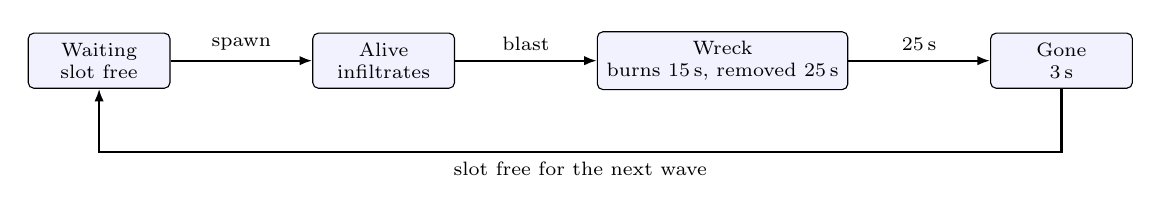
\begin{tikzpicture}[node distance=14mm and 18mm, every node/.style={font=\scriptsize},
  st/.style={draw,rounded corners=2pt,minimum height=7mm,minimum width=18mm,align=center,fill=blue!5},
  arr/.style={-{Latex[length=1.6mm]},thick}]
  \node[st] (w) {Waiting\\slot free};
  \node[st,right=of w] (a) {Alive\\infiltrates};
  \node[st,right=of a] (r) {Wreck\\burns 15\,s, removed 25\,s};
  \node[st,right=of r] (g) {Gone\\3\,s};
  \draw[arr] (w) -- node[above]{spawn} (a);
  \draw[arr] (a) -- node[above]{blast} (r);
  \draw[arr] (r) -- node[above]{25\,s} (g);
  \draw[arr] (g.south) -- ++(0,-8mm) -| node[pos=0.25,below]{slot free for the next wave} (w.south);
\end{tikzpicture}
\caption{Intruder life cycle (\code{Intruder::Life}); constants \code{kWreckBurnTime}=15\,s, \code{kWreckClearTime}=25\,s,
\code{kRespawnDelay}=3\,s; a breach returns the slot directly to Waiting.}
\label{fig:life}
\end{figure}

\begin{itemize}
  \item \textbf{Alive.} The rover infiltrates (Section~\ref{sec:rover}); heat footprints are laid under its wheels and the parked hull. Damage slows it and, below 60 HP, makes it smoke.
  \item \textbf{Wreck.} \code{destroyIntruder()} counts a kill, stops the rover, tells the squad to ignore the wreck, saves every part's material and replaces it by a charred one
  (albedo $\times0.1+(0.015,0.013,0.012)$, roughness 0.95, metalness 0, heat 0.95, no emission), turns all parts except the hull core
  (\emph{Chassis, Upper hull, Motor + battery box}) into rigid-body debris and adds a scorch mark.
  \item \textbf{Burning.} For 15\,s the wreck emits fire, smoke and embers in proportion to the remaining burn fraction;
  the hull cools as $h=0.3+0.65\,e^{-t/40\,\text{s}}$ (visible in the thermal view) and deposits heat on the
  ground (0.25 per second). After 25\,s the wreck is removed and 3\,s later the slot is free; T107 checks wreck $\to$ gone $\to$ alive.
\end{itemize}

\subsection{Engagement rules}\label{sec:engage}
The UAVs' target selection, lock times, friend-or-foe and keep-out rules, wreck discrimination and the combined strike
belong to the squad (Section~\ref{sec:squad}); the thermal detection behind them is Chapter~\ref{sec:vision}. Manual flight
disables the autonomous launch, and \texttt{Enter} releases a rail round at the camera's aim point.

\subsection{Projectiles}
\sheetfig{s16_weapons}
\paragraph{Proportional-navigation homing.} A UAV missile (speed profile in Section~\ref{sec:squad}) homes on its laser spot, the ground point at the centre of the gimbal image. With the spot at
$\vect r$ (vector from the missile), $\hat{\vect v}$ its heading, $V$ its speed and $\hat{\vect l}=\vect r/|\vect r|$ the line of sight,
the commanded turn rate is
\begin{equation}
  \boldsymbol\omega=\frac{4V}{|\vect r|^2}\,(\hat{\vect v}\times\vect r)+2\,(\hat{\vect v}\times\hat{\vect l}),\qquad |\boldsymbol\omega|\le6\ \text{rad/s},
\end{equation}
and the heading is rotated about $\hat{\boldsymbol\omega}$ by $|\boldsymbol\omega|\Delta t$ (Rodrigues' formula). The first term is proportional navigation with $N=4$ for a
stationary spot, the second a heading-error term. The turn limit models limited manoeuvrability. The proximity fuse radius is 0.5\,m, a closest-approach
fuse fires within 3\,m of the spot, and a round self-destructs after 6\,s (T100: a round launched
$30^\circ$ off the line of sight detonates 0.50\,m from the spot after 0.32\,s). Substeps are at most $1/120$\,s.

\paragraph{Ballistic shell.} The tank shell flies at 120\,m/s under gravity without drag; T101 finds a range of 203.8\,m against
$v^2\sin2\alpha/g$ (within $-0.24$\,\%).

\paragraph{Tracer and segment tests.} The AA tracer flies at 1000\,m/s for at most 2.5\,s with no blast at burn-out. At 1000\,m/s a round moves 16.7\,m per
$1/60$\,s step, so impacts are tested as \emph{segments} from the previous to the new position against every target sphere (radius plus fuse), every static solid box
(slab test) and the ground, taking the earliest entry $t\in[0,1]$; nothing tunnels (T102 finds the small target). Blast power: missile 1.0, shell 1.6, tracer 0.15.

\subsection{Blast damage}
\sheetfig{s16_effects}
A blast of power $p$ damages every living intruder within $R=1.6\,p$ metres (\code{kDamageRadiusPerPower}) and the one hit directly. An armoured rover has
\code{kRoverHealth}\,$=100$ HP and loses $30\,p\,(1-\tfrac12\min(d/R,1))$ per blast ($d=0$ for a direct hit), so four direct power-1 hits destroy it (T105: five hits to kill, nothing at $3\,R$);
earlier hits only raise an \code{EnemyHit} event, sparks and dust. Controllable objects within $6\,p$ metres receive \code{onBlast()}; the tank and the AA gun scorch (darken their camouflage). A blast with $p\ge0.3$
spawns a flash (0.12\,s), a fireball of 10--25 fire puffs, a smoke column of 15--40 puffs with a 6--12\,s life, 30--60 sparks, 8--15 embers, a ground shock-wave ring, 10--20 dust
puffs, a decaying point light, camera shake within 25\,m (decaying over 0.8\,s) and a scorch mark of radius $0.9\,p$ (cap 96 marks, 120\,s life). T103 checks that all seven main
particle types appear, the light decays 1 $\to$ 0 and one scorch is left.

\subsection{Rigid-body debris}
Each non-core part becomes an independent rigid body. At the moment of the blast the part's world matrix $W_0$ and origin $\vect c_0$ are stored. The initial velocity points
away from the blast with a lift,
$\vect v_0=\mathrm{normalize}(\vect a+\text{jitter})\,(2.5+3.5\,r)\sqrt p+(0,1.5+3r',0)$ with $\vect a=\vect c_0-\vect b$, its $y$ component clamped to $\ge0$ and raised by 0.6\,m, and the spin has a pseudo-random axis and a rate of
4--14\,rad/s. Each substep ($\le1/120$\,s) applies gravity, moves the body, and composes the rotation with a Rodrigues rotation about the spin axis. The world matrix is
\begin{equation}
  W(t)=T(\vect c(t))\,R(t)\,T(-\vect c_0)\,W_0 ,
\end{equation}
i.e.\ the part is rotated about its own origin and moved to the integrated position. On ground contact (terrain $+0.03$\,m): restitution 0.3 in the normal direction,
horizontal speed $\times0.7$ and spin $\times0.6$ per contact; a piece comes to rest below 0.25\,m/s. T106: 23 pieces, peak height 3.25\,m, all at rest on top of the terrain within
8\,s. Because the hull core stays and the other 23 parts fly, a wreck keeps a recognisable chassis.

\begin{figure}[h]
  \centering
  \begin{subfigure}{0.325\linewidth}\picfour{thermal_fpv_strike}{\linewidth}\caption{Thermal FPV at the strike}\end{subfigure}
  \begin{subfigure}{0.325\linewidth}\picfour{uav_missile_launch}{\linewidth}\caption{Missile launch}\end{subfigure}
  \begin{subfigure}{0.325\linewidth}\picfour{explosion_early}{\linewidth}\caption{Explosion, +0.15\,s}\end{subfigure}\\[1mm]
  \begin{subfigure}{0.325\linewidth}\picfour{explosion_mid}{\linewidth}\caption{Explosion, +1\,s}\end{subfigure}
  \begin{subfigure}{0.325\linewidth}\picfour{explosion_smoke}{\linewidth}\caption{Smoke column, +5\,s}\end{subfigure}
  \begin{subfigure}{0.325\linewidth}\picfour{wreck_burning}{\linewidth}\caption{Burning wreck, +9\,s}\end{subfigure}
  \caption{The strike sequence (captures at the delays set in \code{Capture.cpp}).}
  \label{fig:strike}
\end{figure}


% =====================================================================
\section{The Walkable Bunker}\label{sec:walk}
The command bunker is underground, so the player walks into it. Two CPU-only, unit-tested pieces implement this (T50--T54, T60--T69, T120--T126): the \code{WalkSpace}
(floors, walls and indoor volumes, \code{scene/WalkSpace.h}, built by \code{Bunker.cpp}) and the \emph{walk camera} (\code{Camera::moveWalk}).

\subsection{WalkSpace}
\begin{itemize}
  \item \textbf{Floors.} A \code{WalkFloor} is a rectangle with a floor height at its low and high edge along a slope axis (flat, $x$ or $z$) and a ceiling
  height. The bunker defines 12: the entrance ramp (a linear slope along $z$ from the surface at $z=13$ to $-3.4$\,m at $z=6$), a level
  approach, the door zone, the tunnel, the CIC opening, the command room ($x\in[-5.2,5.2]$, $z\in[-8.2,-2.1]$), the bunk room and doorway, the generator room and doorway, the shaft entrance and the exit shaft.
  Outside every floor the walker stands on the terrain.
  \item \textbf{Which floor.} \code{floorHeight(x,z,feetY)} returns the \emph{highest} floor containing $(x,z)$ that is at most a 0.45\,m step above the feet
  and whose ceiling is above the feet, so a walker on the mound above the rooms stays on the terrain and one in the tunnel is not pulled onto the roof.
  \item \textbf{Walls.} 36 axis-aligned boxes (retaining and cross walls, furniture, jambs). \code{collide()} pushes a vertical cylinder (radius 0.3\,m) out of every box, in two passes
  to settle corners; boxes below the feet or above the head are ignored.
  \item \textbf{Dynamic obstacles.} The closed blast door and a lowered barrier arm are extra boxes each frame (T64, T121).
  \item \textbf{Indoor volumes.} Five boxes (tunnel, CIC, bunk, generator, shaft) form the shader's indoor mask (Section~\ref{sec:shading}).
\end{itemize}
The bunker part budget in test T66 reads: \bunkerBudget. T69: 12 floors, 36 walls, 5 indoor volumes.

\subsection{Walk camera}
Key \texttt{C} cycles Orbit, Free, Chase, UAV CAM and Walk (T55). In walk mode the eye is 1.7\,m above the feet (T51: maximum deviation 0.013\,m over 2\,400 steps), the field of
view $60^\circ$, the speed 1.6\,m/s (4.5 with Shift). Steps are split into $\le0.15$\,m pieces so a fast frame cannot tunnel through a door, and the feet follow the floor after each piece
(T120: ramp deviation 0\,m). The eye stays 0.15\,m below the ceiling (T123), pitch is clamped to $\pm80^\circ$ (T54), the position to a 52\,m radius (T53), and the walker cannot fall into the trench (T52).
A small head bob is added to the rendered eye only.

\subsection{Verified walk-through}
T62 walks from the ramp top to the CIC centre in 367 steps with 0 wall contacts, a maximum step of 0.023\,m and a minimum head room of 2.60\,m. T121: with the doors closed the walker stops at
$z=4.4$\,m (door plane $z=4$) and stays on the ramp ($|x|\le1.2$\,m). T122: with the doors open he reaches the CIC ($z=-6.0$\,m, feet $-3.40$\,m, smallest ceiling gap 0.90\,m).
T126: the director's bunker shot ends in the rooms with a maximum vertical step of 0.118\,m, and T129 checks that the director opens the doors early.

\begin{figure}[h]
  \centering
  \begin{subfigure}{0.49\linewidth}\picfour{bunker_ramp}{\linewidth}\caption{Entrance ramp (walk camera)}\end{subfigure}
  \begin{subfigure}{0.49\linewidth}\picfour{bunker_door}{\linewidth}\caption{Blast doors}\end{subfigure}\\[1mm]
  \begin{subfigure}{0.49\linewidth}\picfour{bunker_tunnel}{\linewidth}\caption{Tunnel}\end{subfigure}
  \begin{subfigure}{0.49\linewidth}\picfour{bunker_cic}{\linewidth}\caption{Command room (CIC)}\end{subfigure}
  \caption{Walking into the bunker (captures \code{bunker\_*}; eye heights 1.7\,m).}
  \label{fig:bunkerwalk}
\end{figure}

% =====================================================================
\section{Platform, Build and Running on the RTX 4070}\label{sec:platform}
The source is C++17 with GLFW (window) or EGL (headless), GLAD (OpenGL 3.3 core loader) and no other library. The Makefile targets are \code{all}, \code{test}, \code{docs} (export, tests, workbook), \code{run} and \code{clean};
\code{HEADLESS=1}, \code{CXX}, \code{CC}, \code{OBJ}, \code{APP} and \code{TESTS} select the build.

\begin{table}[h]
\centering\small
\caption{Build routes. ``Verified'' means done in the development environment (Linux/WSL with a Mesa llvmpipe software GPU).}
\label{tab:build}
\begin{tabular}{@{}p{3.1cm}p{7.6cm}p{4.6cm}@{}}
\toprule
Route & Command & State\\\midrule
Windows one click (MinGW-w64) & \code{run.bat} (builds \code{ThermalSense.exe} if missing, then starts it; arguments pass through) & not run here (no Windows machine)\\
Windows make & \code{mingw32-make -j8} (also builds the tests) & not run here\\
Windows cross-build from Linux & \code{tools/cross\_build\_windows.sh} (zig cc, GLFW linked statically from \code{lib/libglfw3.a}) & cross-link only; the executable has never been run natively\\
Linux with a display & \code{./build.sh} or \code{make -j\$(nproc)}, then \code{./run.sh} (needs \code{libglfw3-dev}, \code{pkg-config}) & GLFW route not exercised here\\
Linux headless (EGL only) & \code{./build.sh -{}-headless} or \code{make HEADLESS=1} & verified (this report's tests)\\
CMake & \code{cmake -B build-cmake \&\& cmake -{}-build build-cmake -j} (\code{-DTS\_HEADLESS\_ONLY=ON} for EGL only) & not re-run\\
Tests (this report) & \code{make -j6 HEADLESS=1 CXX=zcxx CC=zcc OBJ=build/obj-e1 APP=build/ts-e1 TESTS=build/tests-e1 build/tests-e1}\newline\code{./build/tests-e1 build/test\_results.json} & verified: \nTests{} tests, \nFail{} failures\\
Exporter & \code{make docs} $\to$ \code{build/scene\_export.json}, \code{build/test\_results.json} & verified\\\bottomrule
\end{tabular}
\end{table}

\paragraph{Test binary.} The tests link only the CORE sources (no \code{src/app}, no \code{src/rendering}, no GL), so simulation, planner,
combat and walk logic are testable without a GPU. Each area has its own file using the \code{TS\_TEST\_GROUP} macro of
\code{tests/TestKit.h}; the groups are listed in Table~\ref{tab:testareas}.

\subsection{Command-line options}
\begin{table}[h]
\centering\small
\caption{Options (\code{src/main.cpp}, \cli{help}).}
\label{tab:cli}
\begin{tabular}{@{}p{6cm}p{9.8cm}@{}}
\toprule
Option & Meaning\\\midrule
(none) & interactive simulation, F1 lists the controls\\
\cli{capture DIR [-{}-only a,b]} & render the report figures (every shot of \code{shotList()}, or the named ones)\\
\cli{record FILE [SECONDS]} & cinematic video, default 120\,s director sequence (needs ffmpeg)\\
\cli{benchmark FILE} & FPS per preset, per-feature ablation and GPU pass times\\
\cli{trace FILE SECONDS} & UAV / rover behaviour log (4\,Hz CSV)\\
\cli{export-docs FILE} & GPU-free export of every part, matrix and mesh (the exporter binary does the same)\\
\cli{quality low|high|ultra|epic} & preset (default: automatic; EPIC on NVIDIA / discrete GPUs)\\
\cli{size WxH}, \cli{fullscreen} & output size; full screen on the primary monitor\\
\cli{headless}, \cli{gpu N} & EGL context without a window; EGL device index (or environment \code{TS\_EGL\_DEVICE})\\
\cli{fps 30|60}, \cli{encoder NAME}, \cli{ffmpeg PATH} & video frame rate, codec (\code{libx264}, \code{h264\_nvenc}, \code{hevc\_nvenc}) and the ffmpeg executable\\\bottomrule
\end{tabular}
\end{table}

\subsection{Running on the RTX 4070 remote machine}
\begin{enumerate}
  \item \textbf{Windows remote.} Install MinGW-w64, run \code{build.bat} (or rebuild the executable with the cross-build script), then
  \code{run.bat -{}-fullscreen} or \code{run.bat -{}-quality epic -{}-size 2560x1440}. For remote desktop use Parsec or Sunshine + Moonlight, which capture the GPU output. Plain RDP often
  exposes only the Microsoft Basic Render Driver (software), so start the program from a console session or use the headless route.
  \item \textbf{Linux desktop.} \code{sudo apt install build-essential pkg-config libglfw3-dev}; \code{./build.sh \&\& ./run.sh -{}-fullscreen}. On hybrid laptops
  \code{\_\_NV\_PRIME\_RENDER\_OFFLOAD=1 \_\_GLX\_VENDOR\_LIBRARY\_NAME=nvidia ./run.sh}.
  \item \textbf{Linux headless over SSH.} Needs only the NVIDIA driver (EGL) and ffmpeg for video; \code{tools/remote\_setup\_linux.sh} installs everything and builds.
\end{enumerate}
The program logs \code{GL\_RENDERER} at start-up. If it says \code{llvmpipe}, \code{Mesa} or \code{Microsoft Basic Render Driver}, the NVIDIA driver is not in use.

\paragraph{FPS on the RTX 4070 has not been measured.} All captures and tests were produced on a Mesa llvmpipe software renderer, where
a shot takes one to two minutes. To obtain the RTX figures run, on the RTX machine:
\begin{center}\small
\code{ThermalSense -{}-headless -{}-quality epic -{}-benchmark build/benchmark.json}\quad (or without \code{-{}-headless} in a window)
\end{center}
and, for the 4K video, \code{ThermalSense -{}-headless -{}-quality epic -{}-size 3840x2160 -{}-fps 60 -{}-encoder h264\_nvenc -{}-record report/demo\_4k.mp4 60}.
The benchmark writes FPS and ms per frame for each preset, per-feature ablation, draw calls and per-pass GPU times; \code{tools/build\_workbook.py} puts them in the workbook.

\paragraph{Capture shots.} \cli{capture} renders the shots of \code{shotList()} at the sizes set in \code{Capture.cpp}. Each shot sets its own time, camera
and flags; the strike shots are rendered at fixed delays after the impact so that each explosion phase is reproducible.

% =====================================================================
\section{Testing}\label{sec:testing}
\sheetfig{s10_testing}
All tests are CPU-only (no GPU, no window), built and run for this report (Table~\ref{tab:build}); \texttt{build/test\_results.json} holds the id, description, expected and observed text and result of each.
\textbf{\nTests{} tests were run, \nPass{} passed and \nFail{} failed.} Table~\ref{tab:testareas} groups them by area; the complete list is Table~\ref{tab:alltests}
(generated from the JSON by \code{report/gen\_tables.py}).

\begin{table}[h]
\centering\small
\caption{Tests by area (generated).}
\label{tab:testareas}
% generated by report/gen_tables.py -- do not edit
\begin{tabular}{@{}lrr@{}}\toprule
Area (id range) & Tests & Pass\\\midrule
Primitives, transforms, camera maths (T01--T19) & 19 & 19\\
Tracker, occlusion, planner, UAV logic (T20--T32) & 13 & 13\\
Shadows, props, terrain, heat trail, walk camera (T33--T55) & 23 & 23\\
Bunker and terrain (T60--T69) & 10 & 10\\
Base (T70--T79) & 10 & 10\\
Tank and AA gun (T80--T89) & 11 & 11\\
Helicopter and radar (T90--T99) & 10 & 10\\
Combat and game logic (T100--T113) & 14 & 14\\
Application, director, bunker walk (T120--T129) & 10 & 10\\
v5 vision, squad, mission (T130--T149, T180--T189) & 18 & 18\\
v5 hidden camp (T150--T159) & 10 & 10\\
v5 audio (T160--T169) & 12 & 12\\
v5 game HUD (T170--T179) & 9 & 9\\
v6 time of day, sky, clouds (T190--T199) & 10 & 10\\
v6 soldiers (T200--T214) & 15 & 15\\
v6 random routes, day rules (T215--T224) & 10 & 10\\
v6 sensor model, real CV (T225--T236) & 12 & 12\\
v6 CLI, director clock, HUD (T237--T239) & 3 & 3\\
v7 game camera and POV (T240--T259) & 19 & 19\\
v7 ray tracing (T260--T279) & 20 & 20\\
v7 frame explorer (T280--T299) & 20 & 20\\
v7 game audio (T300--T309) & 11 & 11\\
\midrule
Total & 289 & 289\\
\bottomrule
\end{tabular}

\end{table}

Not covered by tests: anything that needs a GPU (rendered output, GLSL compilation, frame time), the interactive keyboard/mouse path in
\code{App}, the HUD drawing and the video encoder. Up to v5 these were checked on captures made with the llvmpipe renderer (Section~\ref{sec:results}); the v6 renderer changes were checked on RTX\,4070 captures, a night regression against the v5 images and 600\,s seeded traces whose rule checks the game emits itself (Section~\ref{sec:v6results}). The v6 tests T190--T239 (Table~\ref{tab:v6tests}) cover the pure functions behind those features: solar geometry and presets, splines, IK, the planner, the roster, random routes, the sensor model and the CV classes; the sensor tests run the real \code{SensorModel} and \code{detectAll} on synthetic frames.
Some test descriptions are stale: T33 reports a shadow texel of 2.15\,cm (a 22\,m sphere at $2048^2$) while the renderer now fits a 39\,m sphere (3.8\,cm). The test
passes but no longer mirrors the renderer (Appendix~\ref{app:audit}).

% generated by report/gen_tables.py from build/test_results.json -- do not edit
{\scriptsize\setlength{\tabcolsep}{2.5pt}
\begin{longtable}{@{}l p{0.52\linewidth} p{0.34\linewidth} c@{}}
\caption{All 289 automated tests (\texttt{build/test\_results.json}). The observed value is abridged to 70 characters; the JSON holds the full text.}\label{tab:alltests}\\
\toprule Id & Description & Observed (abridged) & Result\\\midrule
\endfirsthead
\toprule Id & Description & Observed (abridged) & Result\\\midrule
\endhead
\bottomrule\endfoot
T01 & Cube vertex/\allowbreak{}index count & 24 vertices,\allowbreak{} 36 indices,\allowbreak{} 12 triangles & pass\\
T02 & Cube centred at origin with unit size & min (-0.500,\allowbreak{}-0.500,\allowbreak{}-0.500),\allowbreak{} max (0.500,\allowbreak{}0.500,\allowbreak{}0.500) & pass\\
T03 & Cube normals unit length,\allowbreak{} outward,\allowbreak{} CCW winding & 0 wrong-winding,\allowbreak{} 24/\allowbreak{}24 outward,\allowbreak{} max \textbar{}n\textbar{}-1 = 0.00e+00 & pass\\
T04 & Sphere counts follow 2+(S-1)N vertices and 2N(S-1) triangles (N=36,\allowbreak{} S=18) & 614 vertices,\allowbreak{} 1224 triangles & pass\\
T05 & Sphere vertices lie on r = 0.5 and normal = p /\allowbreak{} r & max radius error 2.98e-08,\allowbreak{} max normal error 0.00e+00 & pass\\
T06 & Sphere lower hemisphere is the reflection (y -\textgreater{} -y) of the upper one,\allowbreak{} CCW kept & 614/\allowbreak{}614 vertices mirrored,\allowbreak{} 0 wrong-winding & pass\\
T07 & Cylinder counts 4N+2 vertices,\allowbreak{} 12N indices (N=36) & 146 vertices,\allowbreak{} 432 indices & pass\\
T08 & Cylinder centred at origin,\allowbreak{} axis along Z,\allowbreak{} radius 0.5,\allowbreak{} height 1 & x [-0.500,\allowbreak{}0.500] y [-0.500,\allowbreak{}0.500] z [-0.500,\allowbreak{}0.500] & pass\\
T09 & Cylinder normals unit length and CCW outward winding & 0 wrong-winding,\allowbreak{} max \textbar{}n\textbar{}-1 = 0.00e+00 & pass\\
T10 & Frustum variant (light cone): open,\allowbreak{} side normals tilted,\allowbreak{} CCW & 0 wrong-winding,\allowbreak{} first normal z = -0.425 & pass\\
T11 & All indices valid and no degenerate triangles & indices valid: yes,\allowbreak{} degenerate: 0 & pass\\
T12 & Indexed storage smaller than non-indexed for every primitive & cube 720\textless{}864,\allowbreak{} sphere 29424\textless{}88128,\allowbreak{} cylinder 5232\textless{}10368 B & pass\\
T13 & Terrain disc: radius 36 m,\allowbreak{} 1+R*N vertices,\allowbreak{} N(2R-1) triangles minus the ramp hole,\allowbreak{} all facing +Y & 49921 vertices,\allowbreak{} 97440 triangles (hole 2016),\allowbreak{} radius 36.00,\allowbreak{} 97440/\allowbreak{}97... & pass\\
T14 & Model matrix order M = T*R*S (scale,\allowbreak{} then rotate,\allowbreak{} then translate) & (1.000,\allowbreak{} 4.000,\allowbreak{} 3.000) & pass\\
T15 & Inverse matrix: inverse(M) * M = I & max error 2.38e-07 & pass\\
T16 & Normal matrix keeps normals perpendicular under non-uniform scale & dot = 0.00e+00 & pass\\
T17 & View-projection maps the look-at target to the NDC centre & ndc (0.000,\allowbreak{} 0.000,\allowbreak{} 0.990) & pass\\
T18 & Bunker,\allowbreak{} UAV and Rover are each built from cube + sphere + cylinder & bunker 400 parts,\allowbreak{} UAV 158 parts,\allowbreak{} rover 156 parts & pass\\
T19 & Shading assignment follows the proposal & all leaves match & pass\\
T20 & All world matrices finite after scene construction & all finite & pass\\
T21 & Searchlight is hierarchical: lamp moves with the UAV body & body moved 0.750 m,\allowbreak{} lamp moved 0.691 m & pass\\
T22 & Tracker finds a hot blob and its centroid & found=1,\allowbreak{} area 24,\allowbreak{} u=0.150 v=0.200 & pass\\
T23 & Tracker ignores single-pixel noise (min area 2) & not found & pass\\
T24 & Data association keeps the existing track instead of a bigger distractor & u=-0.82 v=0.77,\allowbreak{} blobs=2 & pass\\
T25 & Segment/\allowbreak{}box occlusion test & through=1 beside=0 & pass\\
T26 & Visibility grid: behind a tall occluder is hidden,\allowbreak{} on the UAV's side visible & occluder found,\allowbreak{} behind (-11.4,\allowbreak{} -5.3) hidden=1,\allowbreak{} front (-6.9,\allowbreak{} -3.2) v... & pass\\
T27 & Flood fill is a valid BFS field and descent reaches a goal (MicroMouse) & goals 206,\allowbreak{} field consistent 1,\allowbreak{} start value 8,\allowbreak{} path 8 cells,\allowbreak{} end val... & pass\\
T28 & Rover drives (LFR controller) from open ground into the UAV's blind spot within 60 s & hidden=1 at (10.74,\allowbreak{} 3.75),\allowbreak{} travelled 8.4 m,\allowbreak{} line under sensors 723/\allowbreak{}... & pass\\
T29 & Pixel-ray ground estimate: image centre of a downward camera hits the point below it & hit=1 at (0.50,\allowbreak{} -0.05,\allowbreak{} 0.50) & pass\\
T30 & 40 s simulation without detections: UAV searches inside the 20 m area,\allowbreak{} above ground & mode SEARCH,\allowbreak{} inside=1,\allowbreak{} finite=1 & pass\\
T31 & Exact occlusion in primitive space (inverse model matrix),\allowbreak{} not just bounding boxes & sphere corner=0 centre=1,\allowbreak{} cylinder corner=0 body=1 & pass\\
T32 & Hysteresis threshold: a big warm blob without a hot core is not a target & blobs=2,\allowbreak{} found=1,\allowbreak{} u=0.58 v=-0.43,\allowbreak{} area 9 & pass\\
T33 & Moon shadow map: the whole base (39 m world sphere) projects inside the light's clip volume & max \textbar{}NDC\textbar{} = 0.999,\allowbreak{} texel = 3.81 cm & pass\\
T34 & Shadow cascade snapping: moving the camera shifts the shadow map by whole texels only & shift (3.000,\allowbreak{} 0.000) texels,\allowbreak{} fraction 0.0001 & pass\\
T35 & Searchlight shadow matrix: lamp axis -\textgreater{} map centre,\allowbreak{} 14 deg cone edge inside the map & axis (0.000,\allowbreak{} 0.000),\allowbreak{} edge (0.870,\allowbreak{} 0.000) & pass\\
T36 & Cone (cylinder generator,\allowbreak{} top radius 0): counts,\allowbreak{} centred,\allowbreak{} CCW,\allowbreak{} closed,\allowbreak{} no degenerate triangles & 109 vertices,\allowbreak{} 72 triangles,\allowbreak{} x [-0.500,\allowbreak{}0.500] y [-0.500,\allowbreak{}0.500] z [-0... & pass\\
T37 & Exact cone occlusion in primitive space (pine crowns) & near apex=0,\allowbreak{} axis=1,\allowbreak{} base=1 & pass\\
T38 & New props and backdrop are built only from cube /\allowbreak{} sphere /\allowbreak{} cylinder /\allowbreak{} cone leaves & environment 652 parts \{Cube Sphere Cylinder Cone\},\allowbreak{} backdrop 120 par... & pass\\
T39 & Every material has PBR parameters (roughness,\allowbreak{} metalness in [0,\allowbreak{}1]) and all matrices are finite & all leaves OK & pass\\
T40 & Props sit inside the 20 m disc,\allowbreak{} backdrop parts outside it & farthest prop extent 19.57 m,\allowbreak{} nearest backdrop part 38.01 m & pass\\
T41 & No static ground-level prop is hotter than the rover's motor box or reaches the tracker blob threshold & hottest ground-level part Environment/\allowbreak{}Fire embers = 0.74 & pass\\
T42 & Terrain v2: continuous,\allowbreak{} level bunker pad,\allowbreak{} creek bed,\allowbreak{} track depression,\allowbreak{} berm,\allowbreak{} constant rim & max 1 cm step 0.0055 m,\allowbreak{} pad 0.00000 m,\allowbreak{} creek -0.41 m,\allowbreak{} track -0.03 m... & pass\\
T43 & Terrain mesh density and far-ground clearance & radial 0.277 m,\allowbreak{} rim 0.589 m,\allowbreak{} 49921 vertices,\allowbreak{} 97440 triangles,\allowbreak{} min h... & pass\\
T44 & Bucket-grid line of sight equals the brute-force test over all occluders & 0 mismatches,\allowbreak{} 1653 blocked,\allowbreak{} 517 occluders & pass\\
T45 & 180 s headless run: UAV inside 19.5 m and above ground,\allowbreak{} rover finite inside the free area & UAV max r 15.68 m,\allowbreak{} min clearance 7.28 m; rover max r 10.50 m,\allowbreak{} hidde... & pass\\
T46 & UAV mode logic on the 20 m map: detections -\textgreater{} TRACK,\allowbreak{} loss -\textgreater{} REACQUIRE,\allowbreak{} stays inside & track=1 reacquire=1 inside=1,\allowbreak{} estimate (7.3,\allowbreak{} 2.6) & pass\\
T47 & Heat trail cools exponentially: after tau = 45 s a footprint keeps 1/\allowbreak{}e of its heat & start 0.745,\allowbreak{} after 45 s 0.274,\allowbreak{} ratio 0.368 & pass\\
T48 & Heat trail: deposits are local,\allowbreak{} clamped to 1,\allowbreak{} and hot ground stays below the 0.80 blob threshold & centre 1.00,\allowbreak{} 0.5 m away 0.00,\allowbreak{} max ground heat 0.51 & pass\\
T49 & Scene: after 20 s of driving the rover has left a heat trail on the ground & trail peak 0.99,\allowbreak{} rover at (6.1,\allowbreak{} 5.2) & pass\\
T50 & cameraModeName(Walk) is WALK and Walk comes after Cinematic (existing values unchanged) & "WALK",\allowbreak{} Cinematic = 4,\allowbreak{} Walk = 5 & pass\\
T51 & Walk camera: eye height stays 1.7 +- 0.05 m above the terrain while walking and running & max deviation 0.013 m over 2400 steps & pass\\
T52 & Walk camera cannot fall into the open entrance trench from the side (rails /\allowbreak{} retaining wall) & min x 2.15 m,\allowbreak{} lowest feet -0.08 m & pass\\
T53 & Walk camera is clamped to a 52 m radius & radius 52.00 m,\allowbreak{} eye 1.40 m,\allowbreak{} apron -0.30 m & pass\\
T54 & Walk camera: compute() view sits at the walker (eye 1.7 m up) and mouse-look pitch clamps to +-80 deg & dx 0.000 dz 0.000 dy 0.000,\allowbreak{} pitch 80.0 & pass\\
T55 & C cycles Orbit,\allowbreak{} Free,\allowbreak{} Chase,\allowbreak{} UAV CAM,\allowbreak{} Walk,\allowbreak{} back to Orbit & ORBIT\textgreater{}FREE\textgreater{}CHASE\textgreater{}UAV CAM\textgreater{}WALK\textgreater{}ORBIT & pass\\
T60 & Terrain covers the underground rooms with at least 0.15 m of earth & minimum terrain height -0.217 m & pass\\
T61 & Terrain mesh: 36 m radius,\allowbreak{} hole cut for the entrance trench & 0 inside,\allowbreak{} 1398 around,\allowbreak{} radius 36.00,\allowbreak{} 49921 vertices,\allowbreak{} 97440 triangles & pass\\
T62 & Walk from the ramp top to the command room centre stays on the floors & 367 steps,\allowbreak{} 0 contacts,\allowbreak{} max step 0.023 m,\allowbreak{} final y -3.40 (CIC -3.40),\allowbreak{}... & pass\\
T63 & Collision pushes the walker out of walls and furniture; the surface above is free & wall 1 x=-1.20,\allowbreak{} cross 1,\allowbreak{} console 1,\allowbreak{} roof contact 0 & pass\\
T64 & A closed blast door blocks the walker,\allowbreak{} an open one lets him pass & open z=-2.50,\allowbreak{} closed z=4.30,\allowbreak{} reopened z=-2.50 & pass\\
T65 & Blast door state machine OPEN/\allowbreak{}CLOSING/\allowbreak{}CLOSED/\allowbreak{}OPENING,\allowbreak{} \textasciitilde{}4 s travel,\allowbreak{} reversible & BLAST DOORS OPEN 100\% \textbar{} BLAST DOORS CLOSING 100\% \textbar{} BLAST DOORS CLOS... & pass\\
T66 & Bunker part budget & 400 parts: Blast door assembly 28,\allowbreak{} Bunk room 28,\allowbreak{} Bunker shell 21,\allowbreak{} C... & pass\\
T67 & Bunker parts are lab primitives with name and purpose,\allowbreak{} Flat shading,\allowbreak{} occluders only above ground & 0 foreign,\allowbreak{} 0 undocumented,\allowbreak{} 400/\allowbreak{}400 flat,\allowbreak{} 11 occluders (0 buried) & pass\\
T68 & Rig interface: fans,\allowbreak{} beacon above ground,\allowbreak{} ramp cube matches the walk floor,\allowbreak{} door camera & fans 1,\allowbreak{} beacon y 4.30,\allowbreak{} ramp error 0.000 m,\allowbreak{} eye (0.0 -0.3 9.0) & pass\\
T69 & Walk space inventory & 12 floors,\allowbreak{} 36 walls,\allowbreak{} 5 indoor volumes,\allowbreak{} outside height 0.091 (terrai... & pass\\
T70 & every Base part is a lab primitive with a name and purpose & 1335 parts,\allowbreak{} 0 violations & pass\\
T71 & no Base part intersects the helipad,\allowbreak{} radar,\allowbreak{} AA pit,\allowbreak{} tank spot,\allowbreak{} road or trench strip & 0 hits  & pass\\
T72 & perimeter wall is closed except one gate opening centred on +Z (90 deg),\allowbreak{} 9..11 m wide & 204 cells; largest gap 11.0 m at 90.8 deg,\allowbreak{} next 1.00 m & pass\\
T73 & boom barrier: 0 to 85 deg in 2.5 s with smoothstep easing,\allowbreak{} arm box only when lowered,\allowbreak{} input toggles & travel 2.50 s,\allowbreak{} half-way at 1.25 s,\allowbreak{} final 85.0 deg,\allowbreak{} tip y 6.04,\allowbreak{} clos... & pass\\
T74 & waving flag: travelling wave,\allowbreak{} strip rotations bounded,\allowbreak{} flag never stretches or collapses & 12 strips,\allowbreak{} max strip yaw 6.0 deg,\allowbreak{} pitch 1.5 deg,\allowbreak{} tip distance 2.50.... & pass\\
T75 & windsock: 5 hierarchical cone segments that droop more in weak wind & 5 chained segments,\allowbreak{} segment pitch 16.0 deg at wind 0.36 vs 0.7 deg... & pass\\
T76 & Base part counts (static apron + controllables) & static 1253 + controllable 82 = 1335,\allowbreak{} 3 controllables & pass\\
T77 & Base parts are never occluders and stay on the terrain mesh & occluders 0,\allowbreak{} parts beyond r = 36: 0,\allowbreak{} farthest centre 35.5 m & pass\\
T78 & compound: trench strip and bunker footprint free of props; \textgreater{}= 70\% of the v3 occluders kept & strip 0,\allowbreak{} footprint 0 ,\allowbreak{} occluders 506 (v3: 477) & pass\\
T79 & backdrop starts beyond the terrain mesh (r \textgreater{}= 36) and its ground stays just below the apron level & nearest 38.0 m,\allowbreak{} far ground top -0.35,\allowbreak{} solid flags 0 & pass\\
T80 & all 80 track links stay on the track path while driving & max distance 0.00000 m,\allowbreak{} parts: 255 (tracks 80) & pass\\
T81 & track belt advances by speed*dt (link 0 sits at its arc-length position) & advance 16.0000 m vs 16.0000 m (v=8.00 m/\allowbreak{}s,\allowbreak{} perimeter 14.342 m),\allowbreak{} li... & pass\\
T82 & skid steer: equal track speeds drive a straight line & yaw change 0.0000 deg,\allowbreak{} path bearing 30.00 deg (heading 30),\allowbreak{} distanc... & pass\\
T83 & skid steer: opposite track speeds pivot with yaw rate (vr - vl) /\allowbreak{} track width & -62.50 deg/\allowbreak{}s vs -62.50 deg/\allowbreak{}s (vl 1.20,\allowbreak{} vr -1.20),\allowbreak{} drift 0.120 m & pass\\
T84 & turret slews 40 deg/\allowbreak{}s,\allowbreak{} gun 20 deg/\allowbreak{}s,\allowbreak{} elevation limited to -8..+20 deg & yaw 40.0 deg/\allowbreak{}s,\allowbreak{} pitch after 1 s 20.0,\allowbreak{} max 20.00,\allowbreak{} min -8.00,\allowbreak{} huge mo... & pass\\
T84b & turret stays stabilised when the hull turns while possessed & hull yaw -114.8 deg,\allowbreak{} turret world yaw -40.000 -\textgreater{} -40.000 & pass\\
T85 & main gun: 120 m/\allowbreak{}s shell,\allowbreak{} 0.35 m recoil returning in 0.6 s,\allowbreak{} 3.5 s reload,\allowbreak{} 18 rounds & shells 1 at 120.0 m/\allowbreak{}s,\allowbreak{} recoil peak 0.350,\allowbreak{} after 0.0000,\allowbreak{} rounds afte... & pass\\
T86 & hull height follows the terrain (mean of the 4 track corners) & worst error 0.0023 m (terrain relief under the hull up to 0.41 m) & pass\\
T87 & collision against an obstacle box stops the tank; perimeter limit r \textless{}= 31 m & front edge z 7.999 m,\allowbreak{} speed 0.00 m/\allowbreak{}s; perimeter run r = 31.000 m & pass\\
T88 & AA gun: 0.5 s spin-up,\allowbreak{} then 30 rounds/\allowbreak{}s,\allowbreak{} spin coasts down in 1.5 s & first round at 0.517 s,\allowbreak{} 60 rounds in 2 s,\allowbreak{} spin 5.00 -\textgreater{} 2.50 -\textgreater{} 0.00... & pass\\
T89 & AA gun: elevation -5..+85 deg,\allowbreak{} 60 deg/\allowbreak{}s azimuth,\allowbreak{} idle sweep never fires & pitch max 85.00 min -5.00,\allowbreak{} azimuth 60.0 deg/\allowbreak{}s,\allowbreak{} idle: moved 157.4 de... & pass\\
T90 & helicopter rotor spools up in \textasciitilde{}6 s after the start command & rest 0\%,\allowbreak{} startup 1,\allowbreak{} ready after 6.00 s,\allowbreak{} rotor 100\% & pass\\
T91 & 5 blades evenly spaced (72 deg) and the angle integrates rpm * dt & spool 5445,\allowbreak{} 2 s 3600.0,\allowbreak{} spacing error 0.000,\allowbreak{} blade1 45.0 vs 45.0 & pass\\
T92 & attitude follows acceleration but stays bounded; speed capped at 25 m/\allowbreak{}s & max pitch 22.2,\allowbreak{} roll 25.5,\allowbreak{} nose-down 21.7,\allowbreak{} speed 24.5 m/\allowbreak{}s & pass\\
T93 & altitude limited to 0.5..40 m AGL while airborne,\allowbreak{} radius \textless{}= 60 m & max AGL 40.00,\allowbreak{} min AGL 0.50,\allowbreak{} max r 60.00 & pass\\
T94 & landing only from low speed /\allowbreak{} height on flat ground; touches down and spools down & high 1,\allowbreak{} fast 1,\allowbreak{} accepted 1,\allowbreak{} parked 1,\allowbreak{} rotor 0\%,\allowbreak{} steepest slope 0.31... & pass\\
T95 & not possessed: parked helicopter stays still; released in flight it hovers in place & parked still 1; flying: speed 0.00,\allowbreak{} alt 14.5 -\textgreater{} 14.5,\allowbreak{} drift 0.019,\allowbreak{}... & pass\\
T96 & helicopter: lab primitives only,\allowbreak{} every node named,\allowbreak{} blur disc fades in,\allowbreak{} parked on the pad with an obstacle box & leaves 91,\allowbreak{} lab 1,\allowbreak{} named 1,\allowbreak{} blur 0.00 -\textgreater{} 0.26,\allowbreak{} boxes 2,\allowbreak{} pos (20.3,\allowbreak{} 1... & pass\\
T97 & radar ROTATE mode turns 12 rpm (360 deg in 5 s) & swept 360.00 deg in 5 s,\allowbreak{} mode ROTATE & pass\\
T98 & radar SECTOR mode sweeps +-45 deg around the aimed centre & mode SECTOR,\allowbreak{} centre 165.6,\allowbreak{} range -45.0 .. 45.0 & pass\\
T99 & radar tilt limited to -5..+20 deg; antenna = 7 x 3 curved tiles; lab primitives only & tilt -5.0 .. 20.0,\allowbreak{} tiles 21,\allowbreak{} leaves 108,\allowbreak{} lab 1,\allowbreak{} named 1 & pass\\
T100 & Homing round launched 30 deg off the line of sight detonates within 0.6 m of the laser spot & blast yes at 0.32 s,\allowbreak{} 0.50 m from the spot & pass\\
T101 & Tank shell is ballistic: range on level ground matches v\textasciicircum{}2 sin(2a)/\allowbreak{}g within 2\% & 203.8 m (-0.24\%) & pass\\
T102 & A tracer cannot tunnel through a small target (segment vs sphere per step) & direct hit id 7 & pass\\
T103 & Explosion: fire,\allowbreak{} smoke,\allowbreak{} sparks,\allowbreak{} flash,\allowbreak{} shock wave,\allowbreak{} dust,\allowbreak{} embers + decaying light + scorch & 7 types,\allowbreak{} light 1 -\textgreater{} 0,\allowbreak{} 1 scorch,\allowbreak{} shake 0.81 & pass\\
T104 & Particle count never exceeds the cap (oldest smoke dropped first) & 4000 & pass\\
T105 & Armoured rover: blasts at 0.5 r damage it (hit events),\allowbreak{} it dies on the 4th-5th hit; 3 r: no damage & hits to kill 5,\allowbreak{} hit events 4,\allowbreak{} far rover untouched 1 (slot 1,\allowbreak{} health... & pass\\
T106 & Debris: rigid pieces thrown up,\allowbreak{} all at rest on (not under) the terrain within 8 s & 23 pieces,\allowbreak{} peak 2.99 m,\allowbreak{} 23 resting,\allowbreak{} 23 above ground & pass\\
T107 & Wreck life cycle: burning wreck -\textgreater{} removed after 25 s -\textgreater{} slot free 3 s later (next wave reuses it) & wreck=1 gone=1 freed=1 & pass\\
T108 & Launcher: no round before the target has been tracked for 1.5 s & first request at 1.53 s (mode TRACK) & pass\\
T109 & Target discrimination: a blob on a known wreck is ignored (no track,\allowbreak{} no launch) & mode SEARCH,\allowbreak{} lock 0.00 s,\allowbreak{} request 0 & pass\\
T110 & Friend-or-foe: blobs within 4.5 m of a friendly vehicle are not targets & mode SEARCH,\allowbreak{} request 0 & pass\\
T111 & Keep-out: no launch at a target on the bunker's own entrance ramp & mode TRACK,\allowbreak{} any request 0 & pass\\
T112 & UAV launcher: 4 rail rounds,\allowbreak{} hidden at launch,\allowbreak{} replaced after the 6 s reload & launched 4,\allowbreak{} ready 0,\allowbreak{} hidden 1; after reload ready 4 visible 1 & pass\\
T113 & Full base simulated 120 s: finite state,\allowbreak{} \textgreater{}= 7 possessable objects (UAV + \textgreater{}= 6 new) & 24 controllables (18 possessable),\allowbreak{} 5414 leaves,\allowbreak{} finite 1,\allowbreak{} kills 0,\allowbreak{}... & pass\\
T120 & Walk camera follows the entrance ramp floor going down (feet on the slope,\allowbreak{} eye 1.7 m above) & max feet deviation 0.000 m,\allowbreak{} max eye deviation 0.013 m,\allowbreak{} z = 6.39 m,\allowbreak{}... & pass\\
T121 & Walk camera cannot pass a closed blast door box and stays inside the ramp walls & stopped at z = 4.400 m,\allowbreak{} max \textbar{}x\textbar{} 1.200 m & pass\\
T122 & With the doors open the walker goes down the ramp,\allowbreak{} through the door and reaches the CIC & z = -6.01 m,\allowbreak{} feet -3.40 m,\allowbreak{} eye -1.70 m,\allowbreak{} smallest ceiling gap 0.90 m & pass\\
T123 & Walk camera is clamped to 52 m from the origin and the eye to 0.15 m under a low ceiling & radius 52.00 m,\allowbreak{} eye 6.350 m & pass\\
T124 & Camera shake: none at amount 0,\allowbreak{} small and repeatable at amount 1 & rest 0.00000,\allowbreak{} shaken 0.0150,\allowbreak{} repeat 0.000000 & pass\\
T125 & Director: v6 cut 120 s /\allowbreak{} 15 shots and v5 cut 120 s /\allowbreak{} 13 shots,\allowbreak{} contiguous (every moment belongs to exactly one shot,\allowbreak{} fade dips at each cut) & v6: length 120.00 s,\allowbreak{} 15 shots,\allowbreak{} sum 120.00 s,\allowbreak{} contiguous 1,\allowbreak{} finite 1... & pass\\
T126 & Director bunker shot: walk path descends the ramp,\allowbreak{} passes the door plane and ends in the rooms & z end -6.00 m,\allowbreak{} eye end -1.71 m,\allowbreak{} lowest eye -1.72 m,\allowbreak{} max vertical st... & pass\\
T127 & Possession keys 5 6 7 8 9 0 map to tank,\allowbreak{} helicopter,\allowbreak{} AA gun,\allowbreak{} radar,\allowbreak{} blast doors,\allowbreak{} UAV (found by name) & keys 1,\allowbreak{} names 1,\allowbreak{} fallback 1 & pass\\
T128 & [ ] cycle all possessable controllables (flag skipped,\allowbreak{} wraps); walk interaction picks the door /\allowbreak{} barrier within 3.5 m & first 1 last 7 wrap 1,\allowbreak{} door 5,\allowbreak{} barrier 6,\allowbreak{} far -1 & pass\\
T129 & Director scripts: v5 cut unchanged (doors,\allowbreak{} helicopter,\allowbreak{} tank,\allowbreak{} AA); v6 cut: helicopter lifts in its shot,\allowbreak{} doors open at dusk,\allowbreak{} nobody possessed during the night battle & v5 ok 1 (slots 4 1 0 2 -1),\allowbreak{} v6 heli slot 1 lift 1.0,\allowbreak{} doors slot 4 a... & pass\\
T130 & CV image stage: 3 hot discs found among 400 speckles,\allowbreak{} centroids exact & 3 targets (3 matched),\allowbreak{} worst centroid error 0.000 px,\allowbreak{} 396 speckle p... & pass\\
T131 & Two-pass union-find labelling merges a U shape into one component & 2 components,\allowbreak{} U label 1 at both tops & pass\\
T132 & Otsu threshold separates a bimodal image; second moments give the bar's axis and elongation & t = 40,\allowbreak{} orientation 0.0 deg,\allowbreak{} elongation 10.3 & pass\\
T133 & Hungarian assignment finds the optimal total cost (vs brute force over 120 permutations) & 50 /\allowbreak{} 50 & pass\\
T134 & Two-view triangulation (closest points of two rays) vs one ray on the ground & triangulated 0.051 m (residual 0.085 m),\allowbreak{} single ray 0.071 m & pass\\
T135 & Kalman tracker: one confirmed track,\allowbreak{} position error \textless{} 0.25 m,\allowbreak{} velocity -\textgreater{} 1.2 m/\allowbreak{}s & 1 tracks,\allowbreak{} state 1,\allowbreak{} vx 1.07 m/\allowbreak{}s,\allowbreak{} late max error 0.164 m & pass\\
T136 & Two crossing targets keep their track IDs; one-frame clutter never becomes a track & ids 1 /\allowbreak{} 2,\allowbreak{} swapped 0,\allowbreak{} clutter confirmed 0,\allowbreak{} tracks 2 & pass\\
T137 & Squad fusion: one target seen by both UAVs -\textgreater{} one track updated by triangulation & 1 tracks,\allowbreak{} 20 fused updates,\allowbreak{} error 0.004 m & pass\\
T138 & Time-on-target model: predicted round flight time vs the simulated round (6 /\allowbreak{} 12 /\allowbreak{} 25 m) & worst error 0.7 \% & pass\\
T139 & Squad patrol: both UAVs inside the compound,\allowbreak{} kept apart (opposite phases) & min separation 21.6 m,\allowbreak{} UAV 0 radius 10.5 m,\allowbreak{} roles PATROL /\allowbreak{} PATROL & pass\\
T140 & Full loop (synthetic vision): tracks -\textgreater{} coordinated strikes -\textgreater{} intruders destroyed & kills 2 (combined 1),\allowbreak{} launched 4 /\allowbreak{} 6,\allowbreak{} score 250,\allowbreak{} wave 2,\allowbreak{} breaches 1... & pass\\
T141 & Combined strike: both UAVs commit and the two rounds detonate together (time on target) & 4 combined strikes,\allowbreak{} closest blast pair 0.00 s,\allowbreak{} 1 combined kills & pass\\
T142 & Two-view fusion is used in the live loop (both UAVs see the same rover) & 672 & pass\\
T143 & Unopposed infiltration: rovers reach camp assets (breach -10 \%),\allowbreak{} the next wave follows & 7 breaches,\allowbreak{} integrity 30 \%,\allowbreak{} waves started 2 (wave 3),\allowbreak{} bases lost 0 & pass\\
T144 & Random routes: two seeds,\allowbreak{} same start /\allowbreak{} objective -\textgreater{} different positions after 25 s,\allowbreak{} both closer & ends 4.31 m apart,\allowbreak{} closed in 11.2 m /\allowbreak{} 6.9 m & pass\\
T145 & Evasion: a UAV within 5 m makes an infiltrating rover hide for 4 s,\allowbreak{} then it resumes & before 0,\allowbreak{} close 1,\allowbreak{} after 0 & pass\\
T150 & launcher,\allowbreak{} parked tank,\allowbreak{} ammo bunker and camp dressing parts are lab primitives with name /\allowbreak{} purpose /\allowbreak{} id & 1459 parts,\allowbreak{} 0 violations; SAM-1 LAUNCHER=112 MLRS-1 ROCKET TRUCK=13... & pass\\
T151 & camp objects keep out of the helipad /\allowbreak{} radar /\allowbreak{} AA pit /\allowbreak{} tank spot /\allowbreak{} road /\allowbreak{} trench strip; bays do not overlap & 0 hits ; 0 overlapping bays & pass\\
T152 & Base /\allowbreak{} Environment /\allowbreak{} Bunker geometry keeps out of the five camp bays and the tank-park revetment & 0 hits  & pass\\
T153 & SAM elevation limited to 0..60 deg,\allowbreak{} turntable to +-170 deg; status line format & EL 60.00 /\allowbreak{} 0.00,\allowbreak{} turntable 170.0 /\allowbreak{} -170.0,\allowbreak{} 'SAM-1  AZ 250  EL 60  R... & pass\\
T154 & SAM elevation follows an eased trapezoid profile: slow start,\allowbreak{} 14 deg/\allowbreak{}s cruise,\allowbreak{} soft stop,\allowbreak{} no overshoot & EL(0.1 s) 0.27,\allowbreak{} EL(1 s) 11.6,\allowbreak{} EL(2 s) 25.6,\allowbreak{} max 45.000,\allowbreak{} reached at... & pass\\
T155 & SAM: no launch while stowed; one canister fires,\allowbreak{} its cap is hidden,\allowbreak{} a round flies,\allowbreak{} smoke is emitted; reload after 8 s & stowed 4/\allowbreak{}4; fire 3/\allowbreak{}4 cap hidden 1 flight 1 particles 55; 7.8 s 3/\allowbreak{}4... & pass\\
T156 & SAM node hierarchy matches the analytic muzzle point (turntable -\textgreater{} cradle -\textgreater{} canister); elevation raises the muzzle & error 0.0000 m,\allowbreak{} muzzle y 4.34 (EL 45) vs 2.70 (stowed) & pass\\
T157 & MLRS ripple: first tube at once,\allowbreak{} then one tube every 0.25 s (12 in about 2.75 s),\allowbreak{} caps hidden,\allowbreak{} smoke emitted,\allowbreak{} reload after the salvo & 1 at 0,\allowbreak{} 5 at 1 s,\allowbreak{} 12 at 3.5 s,\allowbreak{} rippling done 1,\allowbreak{} reload 14.2 s,\allowbreak{} caps... & pass\\
T158 & fewer practical lights on the surface than before (apron + compound + camp),\allowbreak{} much lower total power & before: base 14 + env 7 = 21 (power 1748); after: base 6 + env 4 +... & pass\\
T159 & all camouflage net panels (motor pool,\allowbreak{} bunker trench,\allowbreak{} five camp bays) stay at least 3.2 m above the ground & 297 panels,\allowbreak{} lowest clearance 3.55 m,\allowbreak{} 0 below 3.2 m & pass\\
T160 & all 15 synths are deterministic,\allowbreak{} finite and audible (1e-3 \textless{} peak \textless{} 3) & all ok & pass\\
T161 & explosion energy grows with power & 910.9 \textless{} 2058.6 \textless{} 6396.0 & pass\\
T162 & pan law is equal-power (L\textasciicircum{}2 + R\textasciicircum{}2 = 1),\allowbreak{} hard left /\allowbreak{} right /\allowbreak{} centre & max \textbar{}L2+R2-1\textbar{} = 6.41e-08,\allowbreak{} centre 0.707/\allowbreak{}0.707 & pass\\
T162b & source on the listener's right is louder in the right channel & L -0.000 R 0.300 & pass\\
T163 & attenuation and air-absorption cutoff are monotonic; gain is 1 inside the near clamp & mono 1,\allowbreak{} clamp 1,\allowbreak{} g(30 m) 0.100,\allowbreak{} g(120 m) 0.025 & pass\\
T163b & Doppler: approaching source is pitched up,\allowbreak{} receding down,\allowbreak{} light (within 0.9..1.1) & up 1.048 down 0.960 & pass\\
T164 & offline render length is exactly seconds x 48000 x 2 (and 30 x 1/\allowbreak{}30 s = 1 s) & 0.5 s -\textgreater{} 48000,\allowbreak{} 30 x 1/\allowbreak{}30 s -\textgreater{} 96000 & pass\\
T165 & an explosion event is audible within the next frame (silence before) & pre peak 0.0000,\allowbreak{} onset frame 48,\allowbreak{} peak 0.484 & pass\\
T166 & voice pool never exceeds the limit under 400 one-shots + 40 sources; the loud near blast survives & max 32,\allowbreak{} peak after 0.801 & pass\\
T167 & WAV header is valid (RIFF/\allowbreak{}WAVE/\allowbreak{}fmt/\allowbreak{}data,\allowbreak{} PCM16,\allowbreak{} 48 kHz stereo,\allowbreak{} sizes) and the streaming writer matches & tags 1 fields 1 first sample 8192 stream 1 & pass\\
T168 & master soft limiter keeps the peak below -1 dBFS (0.891) at master volume 2 & peak 0.8680 (-1.23 dBFS) & pass\\
T169 & update(scene) creates the drone rotor voice (and the helicopter /\allowbreak{} tank if present),\allowbreak{} output finite & voices 5,\allowbreak{} peak 0.194,\allowbreak{} finite 1 & pass\\
T170 & Marker projection: the look-at point lands on the screen centre,\allowbreak{} a point behind the camera is not in front,\allowbreak{} a far side point is off-screen & centre (800.0,\allowbreak{} 450.0),\allowbreak{} dist 20.62,\allowbreak{} behind front 0,\allowbreak{} side front 1 onS... & pass\\
T171 & Marker bracket size shrinks with distance,\allowbreak{} is clamped to [10,\allowbreak{} 120] px at 900p and scales with the screen height & 5 m 106.2 px,\allowbreak{} 60 m 10.0 px,\allowbreak{} 60 m at 1800p 20.0 px & pass\\
T172 & Edge arrow: always inside the margin rectangle,\allowbreak{} points outwards; a point to the right sits on the right edge; behind-camera points flip & all inside 1,\allowbreak{} right tip (1570,\allowbreak{} 450),\allowbreak{} behind dir (-1.00,\allowbreak{} -0.00) & pass\\
T173 & Banner timing: wave banner lasts 2.5 s,\allowbreak{} fades in from 0,\allowbreak{} holds at 1,\allowbreak{} fades out monotonically to 0; score pop-ups rise 0 -\textgreater{} 1 & duration 2.50,\allowbreak{} alpha 0.00 1.00 0.50 0.00,\allowbreak{} rise 0.00 -\textgreater{} 1.00 & pass\\
T174 & Event queue: wave /\allowbreak{} spotted (replaced,\allowbreak{} not stacked) /\allowbreak{} kill (+150 combined) /\allowbreak{} hit become banners that expire on time; breach flash decays; BASE LOST then RESTARTING; a clock reset clears all & 4 banners,\allowbreak{} kill ok 1,\allowbreak{} hit gone 1,\allowbreak{} wave gone 1,\allowbreak{} flash 1.00 0.44 0.00... & pass\\
T175 & Mini-map: 180 px across at 900p (360 at 1800p),\allowbreak{} bottom-right; world +x right,\allowbreak{} +z down; the rim is at the world radius; far points are pulled onto the rim & diameter 180 /\allowbreak{} 360,\allowbreak{} centre (1486,\allowbreak{} 770),\allowbreak{} rim dx 90.0 dy 0.0,\allowbreak{} z10 dy... & pass\\
T176 & Integrity bar colour: green at 100 \%,\allowbreak{} amber at 50 \%,\allowbreak{} red at 0 \%; map heading 0 = +z (down the screen),\allowbreak{} 90 deg = +x & 100\%: (0.30 0.95 0.40),\allowbreak{} 50\%: (1.00 0.75 0.15),\allowbreak{} 0\%: (1.00 0.22 0.15)... & pass\\
T177 & Director v6: the night battle,\allowbreak{} dawn,\allowbreak{} day thermal,\allowbreak{} dusk and night shots draw the game HUD (banners); the day camp /\allowbreak{} soldier /\allowbreak{} bunker shots do not & hud flags ok 1,\allowbreak{} finite 1,\allowbreak{} shots 15 & pass\\
T178 & A running mission keeps the HUD queue consistent (no expired or future banners over 20 s); the director-start announcement shows the running wave & consistent 1,\allowbreak{} mission wave 1,\allowbreak{} banner wave 1 & pass\\
T180 & Mission waves: wave n sends min(2 + n,\allowbreak{} 6) rovers from random edge points & wave 1 3 rovers,\allowbreak{} reached wave 6,\allowbreak{} 30 spawns,\allowbreak{} 22 distinct angles & pass\\
T181 & Base integrity: 10 breaches -\textgreater{} BASE LOST,\allowbreak{} restart at wave 1 with full integrity,\allowbreak{} score kept & lost 1,\allowbreak{} integrity 100,\allowbreak{} wave 0,\allowbreak{} score 150 & pass\\
T190 & Solar position (lat 22.8 N,\allowbreak{} decl -4.6): sunrise/\allowbreak{}sunset,\allowbreak{} noon elevation,\allowbreak{} azimuth symmetry & sunrise 06:08 sunset 17:52 noon e 62.60 az 180.0; az 08:00 107.2,\allowbreak{} 1... & pass\\
T191 & Day/\allowbreak{}night gating: waves only in NIGHT (sun \textless{} -6 deg),\allowbreak{} searchlights below -2 deg,\allowbreak{} lamps off by day & 0 violations,\allowbreak{} 228 night samples (11.4 h of waves) & pass\\
T192 & Night preset equals the v5 literals exactly (key = moon,\allowbreak{} ambient,\allowbreak{} sky,\allowbreak{} fog,\allowbreak{} exposure,\allowbreak{} purkinje) & all fields identical at 6 night hours and in Scene\{\} & pass\\
T193 & Day preset: sun key (3.2,\allowbreak{} Kasten-Young colour),\allowbreak{} bright sky,\allowbreak{} thin haze,\allowbreak{} day exposure key,\allowbreak{} no Purkinje & noon I 3.20 col (0.99 0.99 0.97) off 0.40 deg key -2.80 sky.z 0.68;... & pass\\
T194 & Auto cycle period and phase events (Dawn,\allowbreak{} DayBreak,\allowbreak{} Dusk,\allowbreak{} NightFalls once each),\allowbreak{} scrub,\allowbreak{} hysteresis & period 290.6 s; events: Dawn DayBreak Dusk NightFalls ; end 23:00;... & pass\\
T195 & Key-light direction quantised to 1 deg (elevation,\allowbreak{} azimuth): shadow cache re-rendered per quantum & max offset 0.612 deg,\allowbreak{} 25 changes,\allowbreak{} 25 distinct directions & pass\\
T196 & Solar loading only on passive surfaces (heat \textless{} 0.75): noon peak stays below the CV floor 0.80 & 5295 passive leaves,\allowbreak{} peak 0.752 (Fire embers,\allowbreak{} heat 0.74),\allowbreak{} range wor... & pass\\
T197 & SKY /\allowbreak{} TIME OF DAY controllable: W scrubs 2 h/\allowbreak{}s,\allowbreak{} \textbackslash\{\} toggles auto,\allowbreak{} ENTER jumps a phase,\allowbreak{} sun sphere follows & hour 14.000,\allowbreak{} auto 1,\allowbreak{} jumped 1,\allowbreak{} sun error 0.0000 m,\allowbreak{} sun leaf 1 & pass\\
T198 & Cloud layer (120 m,\allowbreak{} coverage \textasciitilde{}0.45) and its shadows: soft,\allowbreak{} drifting with the wind,\allowbreak{} none at night & mean 0.725 (min 0.40 max 1.00); drift err 6.0e-07,\allowbreak{} in-place change... & pass\\
T199 & Auto clock wraps past midnight; HUD clock text 'HH:MM PHASE AUTO\textbar{}MANUAL' & hour 0.802 '00:48 NIGHT AUTO',\allowbreak{} '17:42 DUSK MANUAL',\allowbreak{} 0 events & pass\\
T200 & Centripetal Catmull-Rom: passes the control points,\allowbreak{} G1 joints,\allowbreak{} arc-length table,\allowbreak{} curvature & interp 0.0e+00 m,\allowbreak{} kink 0.063 deg,\allowbreak{} length err 0.003 \%,\allowbreak{} step err 0.00... & pass\\
T201 & Soldier figure: primitives only,\allowbreak{} 34..75 leaves (v7 hero detail),\allowbreak{} depth \textgreater{}= 6,\allowbreak{} capsule limbs,\allowbreak{} unique ids,\allowbreak{} no slot keywords & leaves 75..75,\allowbreak{} depth 7,\allowbreak{} other prims 0,\allowbreak{} capsule mismatches 0,\allowbreak{} ids un... & pass\\
T202 & Gait foot plant: the stance ankle stays fixed in the world (two-link IK on the locked point) & walked 6.1 m,\allowbreak{} 11 plants,\allowbreak{} max drift 0.00 cm & pass\\
T203 & Two-link leg IK: FK(IK(p)) = p for reachable ankle targets,\allowbreak{} clamps beyond reach,\allowbreak{} gait targets reachable & 316/\allowbreak{}360 reachable,\allowbreak{} FK error 8.3e-07 m,\allowbreak{} far target -\textgreater{} false knee 53.... & pass\\
T204 & Gait coordination: legs in anti-phase,\allowbreak{} each arm swings against its leg,\allowbreak{} pelvis bobs twice per cycle & corr legs -0.83,\allowbreak{} corr leg/\allowbreak{}arm -0.93,\allowbreak{} bob peaks 2 & pass\\
T205 & Site planner routes (A* -\textgreater{} string pulling -\textgreater{} Catmull-Rom) keep clear of every obstacle footprint & 17 routes,\allowbreak{} 3820 samples,\allowbreak{} min clearance 0.29 m,\allowbreak{} posts 0.50 m,\allowbreak{} max ra... & pass\\
T206 & Duty roster: by day everyone is outdoors on duty; at night 3 off duty + the technician are in the bunker & day underground 0,\allowbreak{} night underground 4,\allowbreak{} off duty 3,\allowbreak{} night guards 4,\allowbreak{}... & pass\\
T207 & Shift change into the bunker: down the ramp,\allowbreak{} wait at the closed blast doors,\allowbreak{} through the tunnel to the rooms & waiting frames 1002,\allowbreak{} passed closed doors 0,\allowbreak{} wall contacts 0,\allowbreak{} settle... & pass\\
T208 & Possessed soldier: W walks,\allowbreak{} Shift runs,\allowbreak{} solids stop him,\allowbreak{} \textbackslash\{\} cycles crouch /\allowbreak{} wave /\allowbreak{} stand,\allowbreak{} release resumes duty & walked 3.50 m,\allowbreak{} run 3.40 m/\allowbreak{}s,\allowbreak{} stopped at z 21.20 (clearance 0.90),\allowbreak{} C... & pass\\
T209 & Soldier heat: face /\allowbreak{} hands 0.82,\allowbreak{} torso 0.70,\allowbreak{} hottest part below the 0.90 target core; friendly radius 1.2 m & face 0.82,\allowbreak{} hands 0.82,\allowbreak{} torso 0.70,\allowbreak{} max 0.82,\allowbreak{} friendly 1.2 m & pass\\
T210 & Work loops: the mechanic works at both vehicles (wrench shown),\allowbreak{} logistics picks up and sets down crates & mechanic stops MBT-2 ENGINE DECK;HELICOPTER;MBT-2 ENGINE DECK;HELIC... & pass\\
T211 & Blast reaction: a near blast makes the soldier duck (no damage model),\allowbreak{} a far one is ignored,\allowbreak{} then back to duty & near 1 far 0 duck 1,\allowbreak{} pelvis drop 0.50 m,\allowbreak{} shoulder 140 deg,\allowbreak{} recovered 1 & pass\\
T212 & Possession cameras: chase view behind /\allowbreak{} above,\allowbreak{} first-person view at eye height,\allowbreak{} indoor chase under the ceiling & tp back 3.20 m up 2.10 m,\allowbreak{} fp eye 1.62 m,\allowbreak{} indoor eye -1.85 /\allowbreak{} ceiling... & pass\\
T213 & Route speed law v = vmax /\allowbreak{} (1 + 1.5 kappa) and staggered shift departures at dusk & excess 0.00 m/\allowbreak{}s,\allowbreak{} curve min 0.00 /\allowbreak{} straight max 1.24 m/\allowbreak{}s,\allowbreak{} departures... & pass\\
T214 & 300 s of duty with a dusk shift change (seed 42): soldiers keep apart and nobody stays blocked & min distance 0.61 m,\allowbreak{} overlap frames 0,\allowbreak{} long waits 0,\allowbreak{} night roster 8 & pass\\
T215 & Random routes: 0-3 via points in a +-70 deg sector (free cells,\allowbreak{} outermost first); a rover passes them & counts 485/\allowbreak{}519/\allowbreak{}525/\allowbreak{}471,\allowbreak{} 0 bad,\allowbreak{} via passed 2,\allowbreak{} closed in 16.2 m & pass\\
T216 & Route diversity: one spawn /\allowbreak{} objective,\allowbreak{} three random routes -\textgreater{} three different tracks (30 s) & smallest mean separation 1.38 m & pass\\
T217 & Rover personalities: speed 0.8-1.25,\allowbreak{} pause-in-cover \textless{}= 0.5,\allowbreak{} noise lattice 3-7; speed shows & speed 0.80..1.25,\allowbreak{} pause max 0.50,\allowbreak{} noise w 8..40,\allowbreak{} 5 lattices,\allowbreak{} 10 s:... & pass\\
T218 & Objective switch: \textasciitilde{}30 \% of the random routes change to another camp asset part-way & fraction 0.303,\allowbreak{} 0 same,\allowbreak{} objective before 1 after 1 & pass\\
T219 & Spawn ring: uniform bearing outside the north gap,\allowbreak{} radius 16.8 +- 1.2 m; legacy draws unchanged & 0 north,\allowbreak{} 0 off ring,\allowbreak{} worst sector deviation 5.8 \%,\allowbreak{} legacy 1 & pass\\
T220 & Day gating: rover waves only at night (pinned day: none in 40 s; night again: a wave starts) & day: 0 waves,\allowbreak{} 0 rovers; night: 1 waves,\allowbreak{} 2 rovers; noon start rovers 0 & pass\\
T221 & Dawn withdrawal: alive rovers retreat to the fence ring -\textgreater{} Withdraw events,\allowbreak{} not breaches & 3 alive,\allowbreak{} 3 withdrawn (max r 17.1 m,\allowbreak{} last at 15 s),\allowbreak{} 0 breaches,\allowbreak{} inte... & pass\\
T222 & Day lights: searchlight L2,\allowbreak{} both beam cones and UAV 1's light off by day,\allowbreak{} beacon off & night spot/\allowbreak{}beacon 1,\allowbreak{} cones 2,\allowbreak{} lights 1; day spot 0 beacon 0 cones 0... & pass\\
T223 & Seeded patrol: seed 0 = the v5 orbit bit for bit; seeds 7 /\allowbreak{} 8 fly different,\allowbreak{} reproducible orbits & seed 0 identical,\allowbreak{} 7 vs 8 differ 10.6 m,\allowbreak{} repro 1,\allowbreak{} max r 16.3 /\allowbreak{} 16.3... & pass\\
T224 & Friendly marks: per-mark radius (soldier 1.2 m,\allowbreak{} vehicle 4.5 m),\allowbreak{} one per controllable with r \textgreater{} 0 & soldier 1/\allowbreak{}0,\allowbreak{} vehicle 1/\allowbreak{}0,\allowbreak{} 22 marks for 22 controllables (radii matc... & pass\\
T225 & Sensor temporal noise (NETD) from the difference of two flat frames (fixed pattern cancels) & NETD 2.003 DN,\allowbreak{} mean -0.014 DN,\allowbreak{} within 1 sigma 62.2 \% & pass\\
T226 & Fixed-pattern noise (gain,\allowbreak{} offset,\allowbreak{} column stripes) before /\allowbreak{} after the NUC; stuck-hot pixels & raw 2.072 DN (columns 0.750),\allowbreak{} after NUC 0.574 DN (columns 0.189),\allowbreak{} 1... & pass\\
T227 & Optics PSF (3x3 binomial): point source,\allowbreak{} flat field,\allowbreak{} rover core peak & centre 64,\allowbreak{} edge 32,\allowbreak{} corner 16,\allowbreak{} sum 256,\allowbreak{} flat unchanged,\allowbreak{} rover peak... & pass\\
T228 & Rover detection probability under the full sensor model (NETD 2 DN,\allowbreak{} FPN after NUC,\allowbreak{} PSF,\allowbreak{} stuck px) & P\_d 1.000 (300 /\allowbreak{} 300),\allowbreak{} centroid RMS 0.143 px & pass\\
T229 & False targets without a rover (sunlit patch 0.62,\allowbreak{} soldier,\allowbreak{} NETD 2 DN,\allowbreak{} FPN + stuck pixels after the NUC) & 0 false targets,\allowbreak{} 0 hot-clutter blobs in 1000 frames (NUC + bad-pixe... & pass\\
T230 & Persons are never targets: soldier blob (0.80-0.82,\allowbreak{} no core,\allowbreak{} upright) next to a rover & soldier: target 0,\allowbreak{} person 400 /\allowbreak{} 400; rover target 400 /\allowbreak{} 400 & pass\\
T231 & Dropped frames: 1 \% drop rate; the tracker coasts through drops (20 \% + a burst of 3) & drop rate 1.02 \%,\allowbreak{} 57 /\allowbreak{} 300 frames dropped,\allowbreak{} lost 0,\allowbreak{} id changes 0,\allowbreak{} 1... & pass\\
T232 & Gimbal jitter: per-axis sigma 0.08 deg,\allowbreak{} independent axes; jittered camera axis moves accordingly & sigma yaw 0.0794,\allowbreak{} pitch 0.0801 deg,\allowbreak{} corr 0.0031,\allowbreak{} axis RMS 0.1112 de... & pass\\
T233 & Seed reproducibility: same seed -\textgreater{} identical frames,\allowbreak{} jitter,\allowbreak{} drops,\allowbreak{} detections; other seed differs & identical 1,\allowbreak{} detections identical 1,\allowbreak{} seed 78 differs in 86.4 \% of p... & pass\\
T234 & Blind squad never fires: 120 s without vision frames (empty detection),\allowbreak{} rovers infiltrating & 0 rounds launched,\allowbreak{} max tracks 0,\allowbreak{} max rovers alive 3,\allowbreak{} kills 0 & pass\\
T235 & Clutter classes: fire (too big) and tracer (thin) = hot clutter,\allowbreak{} horizontal warm pipe = clutter & targets 0,\allowbreak{} persons 0,\allowbreak{} hot clutter 100,\allowbreak{} clutter 50,\allowbreak{} pipe as clutter... & pass\\
T236 & detectAll: its Target blobs are exactly detectTargets' result (v5 filter unchanged) & 300 /\allowbreak{} 300 frames identical & pass\\
T237 & CLI helpers: --time accepts day /\allowbreak{} night /\allowbreak{} dusk /\allowbreak{} dawn /\allowbreak{} cycle /\allowbreak{} HH:MM and rejects bad values; HUD clock text; run seed never 0,\allowbreak{} differs per clock tick; sun /\allowbreak{} low sun /\allowbreak{} moon glyph & parse 1,\allowbreak{} clock 1,\allowbreak{} seeds 2567648742 2081894225 (repeat 1),\allowbreak{} glyph 1 & pass\\
T238 & v6 director clock: forced at every moment,\allowbreak{} continuous inside shots; night battle,\allowbreak{} dawn time-lapse through -6 deg,\allowbreak{} day camp shots,\allowbreak{} dusk through sunset,\allowbreak{} night finale & forced 1,\allowbreak{} smooth 1,\allowbreak{} battle night 1,\allowbreak{} dawn -12.8 -\textgreater{} 17.3 deg,\allowbreak{} camp da... & pass\\
T239 & v6 HUD: dusk banner replaced by NIGHT FALLS (the shift-change line stays beside it),\allowbreak{} two withdrawals merge into one counted banner; CV boxes map onto the FPV screen (identity at the same FOV,\allowbreak{} x2 when zoomed in,\allowbreak{} centred pillarbox at 16:9); F1 lists F2 /\allowbreak{} ,\allowbreak{} . /\allowbreak{} /\allowbreak{} /\allowbreak{} F3 & dusk 1,\allowbreak{} replaced 1,\allowbreak{} shift kept 1,\allowbreak{} merged 1 (1 banners,\allowbreak{} count 2),\allowbreak{} te... & pass\\
T240 & Game camera poses: quaternion look-at equals lookAt(),\allowbreak{} view \textless{}-\textgreater{} pose round trip,\allowbreak{} slerp ends /\allowbreak{} midpoint,\allowbreak{} world = view\textasciicircum{}-1,\allowbreak{} FOV from the projection & view 9.54e-07,\allowbreak{} round trip 0.000 deg,\allowbreak{} fwd 1.24e-07,\allowbreak{} slerp ends 0.000... & pass\\
T241 & Camera rig blend: starts exactly at the old view,\allowbreak{} ends exactly at the new one after 0.6 s,\allowbreak{} offset decays monotonically (critically damped),\allowbreak{} eases in (no jump on the first frame) & start 0.00e+00,\allowbreak{} end 0.00e+00,\allowbreak{} 36 frames (0.60 s),\allowbreak{} monotone 1,\allowbreak{} first... & pass\\
T242 & Camera rig with a moving target (5 m/\allowbreak{}s): the offset is relative to the target,\allowbreak{} so the camera catches up without overshoot & non-increasing 1,\allowbreak{} final 0.0000 m,\allowbreak{} active 0 & pass\\
T243 & Game feel curves: jump letterbox bump,\allowbreak{} FOV kick with speed (only on boost,\allowbreak{} capped 8 deg),\allowbreak{} hit marker fade,\allowbreak{} frame-rate independent easing & letterbox 1 (mid 0.110),\allowbreak{} kick 1,\allowbreak{} hit 1,\allowbreak{} ease 1 (9.9326 vs 9.9326) & pass\\
T244 & Compass strip: 120 deg over 600 px,\allowbreak{} ticks every 15 deg labelled at 45,\allowbreak{} bearings wrap across north and clamp behind,\allowbreak{} heading 0 = +z & 9 ticks,\allowbreak{} N 1 NE 1 NW 1,\allowbreak{} offset 150.0 (in 1),\allowbreak{} behind -300.0 (in 0),\allowbreak{}... & pass\\
T245 & Free fly camera (Home): glides up to the set speed (0.12 s),\allowbreak{} Shift x3,\allowbreak{} yaw 90 flies along +x,\allowbreak{} stops smoothly,\allowbreak{} wheel speed clamped 1..60 m/\allowbreak{}s & cruise 8.00 (moved 7.11 m),\allowbreak{} boost 23.99 along x 1,\allowbreak{} glide 0.0058,\allowbreak{} wh... & pass\\
T246 & POV sources: every moving object of the v6 scene (8 soldiers,\allowbreak{} both UAVs,\allowbreak{} tank,\allowbreak{} helicopter,\allowbreak{} AA gun,\allowbreak{} SAM + MLRS,\allowbreak{} radar); doors /\allowbreak{} barrier /\allowbreak{} sky clock left out; unique keys,\allowbreak{} stable order & 16 sources: soldiers 8,\allowbreak{} UAVs 2,\allowbreak{} tank 1,\allowbreak{} heli 1,\allowbreak{} AA 1,\allowbreak{} launchers 2,\allowbreak{}... & pass\\
T247 & Every POV source gives a valid camera for every view (first person,\allowbreak{} chase,\allowbreak{} alt): finite,\allowbreak{} unit orientation,\allowbreak{} close to the object,\allowbreak{} sane FOV and near plane & 48 poses checked,\allowbreak{} 0 bad & pass\\
T248 & POV picker: nearest first; row hit test maps every visible row to its list index,\allowbreak{} header /\allowbreak{} margins miss; a long list scrolls to keep the selection visible & ascending 1 (16 entries,\allowbreak{} nearest SOLDIER 1 SENTRY 13.0 m),\allowbreak{} rows 1 (... & pass\\
T249 & Insert /\allowbreak{} Delete cycle every moving object once in the stable order and wrap both ways & visited 16 /\allowbreak{} 16,\allowbreak{} wrap fwd 1 back 1,\allowbreak{} fresh 1 & pass\\
T250 & Middle-click pick: the screen-centre ray picks the object the camera looks at (soldiers,\allowbreak{} UAVs,\allowbreak{} tank),\allowbreak{} the nearer of two on a ray wins,\allowbreak{} a near miss within 4 deg still picks & 11 /\allowbreak{} 11 picked,\allowbreak{} nearer 1,\allowbreak{} miss 1,\allowbreak{} centre ray 1 & pass\\
T251 & Soldier first person: the eyes ride in the head node (gait bob and sway),\allowbreak{} next to the soldier's own eye point,\allowbreak{} looking where he looks & soldier 15,\allowbreak{} bob 0.040 m,\allowbreak{} eye offset 0.084 m,\allowbreak{} angle 0.02 deg & pass\\
T252 & Soldier possession round trip: W walks him (\textasciitilde{}1.5 m in 1.8 s),\allowbreak{} release hands him back to his duty program,\allowbreak{} a second possession turns him again & moved 2.84 m,\allowbreak{} possessable again 1 & pass\\
T253 & Intruder rover round trip: take the wheel (planner paused),\allowbreak{} W drives \textasciitilde{}1.1 m/\allowbreak{}s,\allowbreak{} D turns right (yaw down),\allowbreak{} release gives it back to its planner; still a rover on the field (the UAVs hunt it) & slot 0,\allowbreak{} listed 1,\allowbreak{} moved 2.04 m,\allowbreak{} yaw -0.43 rad,\allowbreak{} AI moved 1.19 m,\allowbreak{} ali... & pass\\
T254 & UAV possession round trip: possessed it flies by hand (PgUp climbs),\allowbreak{} released it returns to the squad's autonomous control & index 0,\allowbreak{} manual 1,\allowbreak{} climb 3.13 m,\allowbreak{} released 1 & pass\\
T255 & Player rover drive: differential drive reaches 1.1 m/\allowbreak{}s (1.8 boosted),\allowbreak{} wheels turn,\allowbreak{} the field edge (19 m) stops it & speed 1.10 m/\allowbreak{}s,\allowbreak{} wheels 1,\allowbreak{} max radius 18.97 m & pass\\
T256 & Round in flight: the follow camera keeps the same missile frame after frame (stable launch-time key) and holds on its impact point when it detonates & 38 frames,\allowbreak{} key stable 1,\allowbreak{} lost 1,\allowbreak{} impact z 27.82 & pass\\
T257 & F1 help and the key table list the v7 game camera keys (F4,\allowbreak{} Home /\allowbreak{} End,\allowbreak{} Insert /\allowbreak{} Delete,\allowbreak{} F11) & F4 1 HOME 1 INS 1 F11 1,\allowbreak{} table 1 (9 rows) & pass\\
T258 & Special cameras: the wing UAV's first person is its thermal gimbal axis,\allowbreak{} its belly camera looks down,\allowbreak{} the rover's bumper camera looks along its heading & gimbal 1,\allowbreak{} belly 1,\allowbreak{} bumper 1 & pass\\
T260 & Ray /\allowbreak{} sphere: quadratic roots (outside,\allowbreak{} inside with unnormalised d,\allowbreak{} miss,\allowbreak{} off-centre) & t = 4.5000,\allowbreak{} 0.2500,\allowbreak{} miss,\allowbreak{} 4.6000 & pass\\
T261 & Ray /\allowbreak{} box: slab method (face normal,\allowbreak{} exit from inside,\allowbreak{} miss,\allowbreak{} axis-parallel ray) & t = 1.5000,\allowbreak{} 0.7071,\allowbreak{} miss,\allowbreak{} 2.5000 & pass\\
T262 & Ray /\allowbreak{} capped cylinder: side quadratic,\allowbreak{} cap planes,\allowbreak{} ray over the top,\allowbreak{} slanted hit on the rim region & t = 2.5000,\allowbreak{} 3.5000,\allowbreak{} miss,\allowbreak{} F = -1.19e-07 & pass\\
T263 & Ray /\allowbreak{} cone: side (exact normal (0.894,\allowbreak{} 0,\allowbreak{} 0.447)),\allowbreak{} base cap,\allowbreak{} hit near the apex,\allowbreak{} no hit on the mirrored nappe & t = 1.7500,\allowbreak{} 2.5000,\allowbreak{} 2.9000,\allowbreak{} n = (0.894,\allowbreak{} 0.447),\allowbreak{} above: miss & pass\\
T264 & Rotated,\allowbreak{} non-uniformly scaled primitives (4000 rays): hit point on the implicit surface,\allowbreak{} normal = its gradient & 2000 hits,\allowbreak{} max \textbar{}F\textbar{} = 3.7e-06,\allowbreak{} max normal error 1.8e-07,\allowbreak{} 0 bad & pass\\
T265 & Terrain height field (2-level DDA,\allowbreak{} 289\textasciicircum{}2 samples): hits lie on terrainHeight(); the trench is a hole & 1979 hits (1.3 cells /\allowbreak{} ray),\allowbreak{} worst 15.4 mm,\allowbreak{} 21 trench rays passed t... & pass\\
T266 & SAH BVH closest hit == brute force over 600 random primitives (20000 random rays) & 0 mismatches,\allowbreak{} 14012 hits,\allowbreak{} 1.8 prim tests /\allowbreak{} ray (brute force: 600),\allowbreak{}... & pass\\
T267 & BVH refit after moving every primitive (and hiding one) stays exact; SAH build beats a median split & 0 mismatches,\allowbreak{} refit cost ratio 1.00,\allowbreak{} SAH 24.9 vs median 37.1 (build... & pass\\
T268 & Fresnel (glass n = 1.5): normal incidence ((n-1)/\allowbreak{}(n+1))\textasciicircum{}2,\allowbreak{} grazing -\textgreater{} 1,\allowbreak{} Brewster angle,\allowbreak{} Schlick vs exact,\allowbreak{} reciprocity & R0 = 0.04000,\allowbreak{} grazing 0.9942,\allowbreak{} Brewster 0.07396 (rs\textasciicircum{}2/\allowbreak{}2 = 0.07396),\allowbreak{}... & pass\\
T269 & Snell's law n1 sin(t1) = n2 sin(t2) (air -\textgreater{} water) and total internal reflection beyond 48.75 deg (water -\textgreater{} air) & max error 1.2e-07,\allowbreak{} TIR classification 998 /\allowbreak{} 998 & pass\\
T270 & Whitted ray tree: glass ball spawns reflection + refraction children (depth limited),\allowbreak{} mirror ball a reflection ray & glass: 11 rays (5 refr,\allowbreak{} 5 refl,\allowbreak{} 0 shadow,\allowbreak{} depth 5); mirror: 4 rays,\allowbreak{}... & pass\\
T271 & White furnace: a convex diffuse sphere (albedo 1 /\allowbreak{} 0.5) under a uniform sky of radiance 1 returns albedo * 1 & 1.0000,\allowbreak{} 0.5000 & pass\\
T272 & Closed furnace (emitting walls Le = 0.1,\allowbreak{} albedo 0.7,\allowbreak{} Russian roulette from bounce 2): L = Le /\allowbreak{} (1 - a) & 0.3333 & pass\\
T273 & Importance sampling is unbiased: GGX + cosine one-sample mix == uniform hemisphere estimate of the albedo & importance 0.4617,\allowbreak{} uniform 0.4607,\allowbreak{} white Lambert (cosine sampling)... & pass\\
T274 & Light tracing (reverse: particles from the lamp,\allowbreak{} camera connections) agrees with path tracing on a small scene & path 0.0734,\allowbreak{} light 0.0733 (0.1\%),\allowbreak{} worst block 2.4\% & pass\\
T275 & Path tracer determinism: same seed -\textgreater{} bit-identical image (1 vs 7 threads); another seed -\textgreater{} different noise & identical,\allowbreak{} different & pass\\
T276 & Scene bridge on the camp: one analytic primitive per solid leaf,\allowbreak{} every primitive reachable,\allowbreak{} refit follows the moving parts & 5400 prims /\allowbreak{} 5400 solid leaves,\allowbreak{} 19 lights,\allowbreak{} 736 /\allowbreak{} 736 centre rays ok... & pass\\
T277 & Ray debugger tree: primary first,\allowbreak{} parents precede children,\allowbreak{} one shadow ray per light,\allowbreak{} contributions add up to the pixel & 4 rays (first primary on floor),\allowbreak{} 2 shadow rays,\allowbreak{} error 0.0e+00 & pass\\
T278 & Render modes cycle raster -\textgreater{} hybrid -\textgreater{} Whitted -\textgreater{} path -\textgreater{} light; std430 GPU records (64/\allowbreak{}48/\allowbreak{}32/\allowbreak{}64 bytes) pack the scene & RASTER \textgreater{} HYBRID RT \textgreater{} WHITTED RT \textgreater{} PATH TRACING \textgreater{} LIGHT TRACING \textgreater{} RA... & pass\\
T279 & Edge-aware a-trous denoiser: removes most of the noise but keeps the normal /\allowbreak{} depth edge sharp & RMSE 0.1303 -\textgreater{} 0.0082,\allowbreak{} edge 0.195 \textbar{} 0.770 (truth 0.2 \textbar{} 0.8) & pass\\
T280 & Frame Explorer stage list: 16 pipeline stages in order,\allowbreak{} each with title,\allowbreak{} caption,\allowbreak{} formula,\allowbreak{} concepts (HUD-printable ASCII) & 16 stages,\allowbreak{} 16 unique,\allowbreak{} order ok & pass\\
T281 & Edge functions /\allowbreak{} 2A are barycentric weights: sum 1,\allowbreak{} reconstruct p,\allowbreak{} inside \textless{}=\textgreater{} all weights \textgreater{}= 0 (both windings) & sum err 1.5e-05,\allowbreak{} reconstruction err 0.0012 px,\allowbreak{} 0 mismatches & pass\\
T282 & Top-left fill rule: interior points on shared edges /\allowbreak{} vertices are covered by exactly one triangle (2-split and 4-fan) & split: 0 double 0 missing; fan: 0 double 0 missing & pass\\
T283 & Perspective-correct interpolation (divide by clip w) matches the ray /\allowbreak{} plane intersection; affine does not & 560 pixels: perspective 0.0002 m,\allowbreak{} affine 39.30 m & pass\\
T284 & Affine and perspective-correct interpolation reproduce vertex values and constant attributes & worst 0 & pass\\
T285 & Vertex trace model -\textgreater{} world -\textgreater{} view -\textgreater{} clip -\textgreater{} NDC -\textgreater{} pixel equals P V M p; points behind the eye are clipped & clip 4.8e-07,\allowbreak{} pixel (1236.73,\allowbreak{} 450.60) vs (1236.73,\allowbreak{} 450.60),\allowbreak{} centre... & pass\\
T286 & Depth: window depth \textless{}-\textgreater{} eye distance round trip; near -\textgreater{} 0,\allowbreak{} far -\textgreater{} 1; matches the projection matrix & round trip 0.00018,\allowbreak{} d(near) 0.00000,\allowbreak{} d(far) 1.00000,\allowbreak{} d(10 m) 0.9950... & pass\\
T287 & Image kernels: blur /\allowbreak{} sharpen /\allowbreak{} emboss /\allowbreak{} identity sum to 1 (brightness kept),\allowbreak{} Sobel /\allowbreak{} Laplacian sum to 0; Gaussian symmetric & identity=1 box blur 3x3=1 Gaussian 5x5=1 Sobel Gx=0 Sobel Gy=0 Sobe... & pass\\
T288 & Convolution: identity keeps the image,\allowbreak{} box keeps a flat image,\allowbreak{} Sobel fires only at a step edge,\allowbreak{} Laplacian of a ramp is 0 & id 0,\allowbreak{} box 0,\allowbreak{} lap 2.4e-07,\allowbreak{} sobel edge 4.00 away 0.00 & pass\\
T289 & Histogram: a grey ramp fills 64 bins evenly; counts sum to the pixel count; channel histograms & sum 257,\allowbreak{} even 1,\allowbreak{} bin13 5,\allowbreak{} red[63] 5 & pass\\
T290 & Halton (2,\allowbreak{}3) sequence of the TAA jitter: textbook values,\allowbreak{} 8 offsets inside the pixel,\allowbreak{} centred & err 0,\allowbreak{} mean (-0.055,\allowbreak{} 0.000) & pass\\
T291 & Tone curve (exposure x 1.6 -\textgreater{} ACES -\textgreater{} sRGB) is monotonic and in [0,\allowbreak{} 1]; sRGB continuous; auto-exposure clamped to +-1.5 EV & mono 1 bounded 1 top 1.000,\allowbreak{} sRGB mono 1 jump 2.5e-06,\allowbreak{} e 2.828 0.354... & pass\\
T292 & Plotted tone curve = the composite shader's ACES fit (input /\allowbreak{} output matrices) on the grey axis & worst 9.7e-06 & pass\\
T293 & Reflection: mirror law (\textbar{}R\textbar{} = 1,\allowbreak{} angle in = out,\allowbreak{} coplanar),\allowbreak{} Schlick F(0) = F0 /\allowbreak{} F(90) = 1,\allowbreak{} CPU SSR march hits the wall where the mirror law says & law 3.6e-07,\allowbreak{} F 0.040 /\allowbreak{} 1.000,\allowbreak{} hit 1 after 37 steps at (0.00,\allowbreak{} 2.79,\allowbreak{}... & pass\\
T294 & Pixel inspector: values at a pixel come from that texel of every buffer (top-left pixel coords -\textgreater{} bottom-up GL rows,\allowbreak{} half-res buffers) & Tank /\allowbreak{} Turret (Cylinder) \textbar{} \#17,\allowbreak{} front face \textbar{} 1.5000 0.2500 0.1250 \textbar{}... & pass\\
T295 & Inspector lists only the buffers that exist and clamps coordinates to the frame & 2 rows,\allowbreak{} first '(0,\allowbreak{} 3)' & pass\\
T296 & Back-face test by the sign of the projected area agrees with the normal test; a cube shows at most 3 faces (\textless{}= 6 front triangles) & 36 /\allowbreak{} 36 agree,\allowbreak{} 14 front & pass\\
T297 & Rasterised pixel count matches the triangle area (within half the perimeter) & 11343 pixels & pass\\
T298 & Planes and depth views use GL order: v = 0 is the bottom row & 4 3 6 & pass\\
T299 & Gamma out = in\textasciicircum{}(1/\allowbreak{}gamma): identity at 1,\allowbreak{} brightens mid-tones for gamma \textgreater{} 1,\allowbreak{} monotonic,\allowbreak{} keeps 0 and 1 & 0.7297 0.3000,\allowbreak{} ends 0.0 1.0,\allowbreak{} mono 1 & pass\\
T300 & all 19 v7 synths (5 footstep surfaces,\allowbreak{} radio,\allowbreak{} 9 UI cues,\allowbreak{} rover,\allowbreak{} generator,\allowbreak{} tank,\allowbreak{} day bed) are deterministic,\allowbreak{} finite and audible & all ok & pass\\
T301 & footstep spectra differ by surface (centroid: gravel /\allowbreak{} concrete \textgreater{}\textgreater{} dirt); surfaceAt() maps bunker,\allowbreak{} helipad,\allowbreak{} road,\allowbreak{} compound,\allowbreak{} outside,\allowbreak{} tower deck & centroid dirt 409 gravel 4761 concrete 1366 metal 1280 grass 3195 H... & pass\\
T302 & HRTF-lite: source at +90 deg -\textgreater{} left ear lags (Woodworth ITD \textless{} 0.7 ms),\allowbreak{} R louder,\allowbreak{} left head shadow; rear source low-passed; rendered: L lags R by the ITD & ITD 31.5 smp (0.656 ms),\allowbreak{} gains L 0.081 R 0.289,\allowbreak{} shadow 1800 Hz,\allowbreak{} rea... & pass\\
T303 & Doppler (physical,\allowbreak{} rendered): rover whine 600 Hz passing at 25 m/\allowbreak{}s -\textgreater{} \textasciitilde{}647 Hz approaching,\allowbreak{} \textasciitilde{}559 Hz receding & measured 646 /\allowbreak{} 560 Hz,\allowbreak{} engine pitch 1.078 /\allowbreak{} 0.933 & pass\\
T304 & master: look-ahead limiter + soft clip keep a 6 s battle below the ceiling; battle loudness -24..-8 dBFS RMS,\allowbreak{} night bed -50..-26 dBFS & peak 0.821,\allowbreak{} limiter min gain 0.72,\allowbreak{} battle -12.0 dBFS,\allowbreak{} night bed -32... & pass\\
T305 & ambience: night = crickets (4.3-5.2 kHz) over the bird band,\allowbreak{} day = birds (1.7-3.9 kHz) up; underground the bed is muffled (2-6 kHz) & cricket/\allowbreak{}bird ratio night 14.0 dB,\allowbreak{} day 1.4 dB; bird band day vs nigh... & pass\\
T306 & ducking: blast at 8.5 m ducks the mix (\textless{} 0.6) within 0.2 s and releases (\textgreater{} 0.95) after 4 s; a blast at 150 m ducks less (\textgreater{} 0.75) & near min 0.35,\allowbreak{} after 4 s 0.999,\allowbreak{} far min 0.90 & pass\\
T307 & bunker zone: listenerBunker() 1 inside /\allowbreak{} 0 outside; inside the beep leaves a long concrete tail; a cannon outside is muffled through the roof (HF/\allowbreak{}LF and level down) & bunker 1.00 /\allowbreak{} 0.00,\allowbreak{} tail -66.2 /\allowbreak{} -79.1 dB,\allowbreak{} HF/\allowbreak{}LF occluded -60.0 vs... & pass\\
T308 & echo taps (image source off the HESCO wall at 34 m and the treeline at 72 m) match the geometry; none inside the bunker; the treeline echo is audible; a blast at 120 m arrives \textasciitilde{}0.29 s late & taps 2 (0.163 s g 0.14,\allowbreak{} 0.385 s g 0.08),\allowbreak{} inside 1,\allowbreak{} pre-wall echo 0.... & pass\\
T309 & whole scene (dusk,\allowbreak{} seed 11): two runs with engine seed 7 are bit-identical,\allowbreak{} seed 8 differs; soldiers' footsteps and phase radio are heard; all 9 UI cues are audible,\allowbreak{} centred and undocked & identical 1 (576000 samples),\allowbreak{} seed 8 differs in 575904,\allowbreak{} footsteps 2... & pass\\
T309b & small arms + possessed vehicle: rifle report deterministic with structure echoes; tracer hits (power \textless{}= 0.2) are short surface ticks that do not duck (metal brighter than dirt); own tank engine through the hull (darker,\allowbreak{} rumble boosted); rover whine follows the throttle & rifle peak 0.50 echo 0.028 det 1; tick 0.08 s duck 1.00 (blast 0.35... & pass\\
\end{longtable}}


% =====================================================================
\section{Game Results}\label{sec:v5results}
\autofig{diagrams}{F10_run_timeline}
\paragraph{Unit tests.} \nTests{} tests were run for this report, \nPass{} passed, \nFail{} failed (Table~\ref{tab:alltests}; ranges T130--T145 vision and squad, T150--T159 camp, T160--T169 audio, T170--T181 HUD and mission).

\paragraph{Headless real-render run.} The real renderer ran headless (\cli{headless}, LOW quality, 90\,s of game time, \cli{trace}) on the Mesa llvmpipe software GPU; the trace is \code{docs/v5\_notes/runs/trace\_v5\_low\_90s.csv}. The program reported \textbf{21 rounds launched, 12 hits, 3 kills (2 of them
combined strikes), wave 2 reached, 47 confirmed tracks and 689 two-view fused track updates}. 12 hits for 3 kills fits the armour rule (4--5 hits per kill). LOW on llvmpipe is not representative of the RTX preset. Before track merging and the flicker-tolerant lock, the same run gave 5 rounds, 0 kills and 48 confirmed tracks: blob flicker created new ids that reset the locks (Sections~\ref{sec:vision}, \ref{sec:squad}). The synthetic-vision test T140 exercises the same loop deterministically on the CPU.

\paragraph{Demo video.} \code{report/demo\_v5.mp4} is 120\,s, $1280\times720$, 30\,fps, H.264 with AAC 48\,kHz stereo audio muxed by \cli{record}, rendered headless on llvmpipe at HIGH quality; it is embedded in the slides.

\begin{figure}[h]
  \centering
  \begin{subfigure}{0.495\linewidth}\picfive{game_overview}{\linewidth}\caption{Game view with HUD}\end{subfigure}
  \begin{subfigure}{0.495\linewidth}\picfive{combined_strike}{\linewidth}\caption{Combined strike: two rounds in flight}\end{subfigure}\\[1mm]
  \begin{subfigure}{0.325\linewidth}\picfive{hit_marker}{\linewidth}\caption{Hit marker}\end{subfigure}
  \begin{subfigure}{0.325\linewidth}\picfive{kill_banner}{\linewidth}\caption{Kill banner}\end{subfigure}
  \begin{subfigure}{0.325\linewidth}\picfive{wave_banner}{\linewidth}\caption{Wave banner}\end{subfigure}\\[1mm]
  \begin{subfigure}{0.6\linewidth}\picfive{tactical_map}{\linewidth}\caption{Tactical map}\end{subfigure}
  \caption{Game captures (event-driven shots of \code{Capture.cpp}).}\label{fig:v5game}
\end{figure}
\begin{figure}[h]
  \centering
  \begin{subfigure}{0.325\linewidth}\picfive{camp_sam}{\linewidth}\caption{SAM launcher under its net}\end{subfigure}
  \begin{subfigure}{0.325\linewidth}\picfive{camp_mlrs}{\linewidth}\caption{MLRS truck}\end{subfigure}
  \begin{subfigure}{0.325\linewidth}\picfive{camp_under_nets}{\linewidth}\caption{Parked tank bay}\end{subfigure}\\[1mm]
  \begin{subfigure}{0.325\linewidth}\picfive{possess_sam}{\linewidth}\caption{Possessing the SAM}\end{subfigure}
  \begin{subfigure}{0.325\linewidth}\picfive{possess_mlrs}{\linewidth}\caption{Possessing the MLRS}\end{subfigure}
  \begin{subfigure}{0.325\linewidth}\picfive{base_overview}{\linewidth}\caption{Hidden camp overview}\end{subfigure}
  \caption{The hidden camp (captures).}\label{fig:v5camp}
\end{figure}

\paragraph{Limits.} FPS on the RTX 4070 is not measured; no benchmark exists. The reflection probe is not implemented. The per-object part-count table was generated before the v5 launchers were exported; re-run \code{gen\_tables.py} after the exporter includes them.

% =====================================================================
\section{Time of Day: Sun, Sky, Clouds and the Day Cycle}\label{sec:daycycle}
\pipestrip{6}
Version~6 replaces the fixed night with a 24-hour clock (\code{scene/DayCycle.\{h,cpp\}}). One scalar, the sun elevation $e$, drives the key light, the sky, fog and exposure, the lamps, the UAV searchlights, the clouds and the game rules (rover waves run only at night). Everything is a pure CPU function of the hour: it is unit-tested (T190--T199), exported (\dcGridRows{} rows of \code{v6.day\_cycle.grid}) and recomputed by Excel formulas in workbook sheet~21 (Figure~\ref{fig:sheet:sheet_daycycle}).

\subsection{Solar position}
The camp sits at latitude $\varphi=\dcLat^\circ$ in early October (declination $\delta=\dcDecl^\circ$). With the hour angle $H=15^\circ\,(h-12)$ the textbook spherical-astronomy relations give the elevation and the unit vector towards the sun in the scene frame ($x$ east, $y$ up, $z$ north):
\begin{equation}
\sin e=\sin\varphi\sin\delta+\cos\varphi\cos\delta\cos H,\qquad
\hat{\vect s}=\bigl(-\cos\delta\sin H,\ \sin e,\ \cos\varphi\sin\delta-\sin\varphi\cos\delta\cos H\bigr),
\end{equation}
and the azimuth from north is $A=\operatorname{atan2}(\hat s_x,\hat s_z)$. Inverting the first relation gives the hour of a given elevation, $h=12\mp\arccos\bigl((\sin e-\sin\varphi\sin\delta)/(\cos\varphi\cos\delta)\bigr)/15^\circ$ (\code{hourAtElevation}). For the camp: sunrise \dcSunrise, sunset \dcSunset, noon elevation $\dcNoonElev^\circ$ due south (T190: \tobs{T190}).
\lstSunDir

\subsection{Phases, clock rate and events}
\autofig{diagrams}{H1_daycycle_curves}
The phase is a band of $e$ with $0.25^\circ$ hysteresis: NIGHT below $\dcNightBelow^\circ$, DAY above $+\dcDayAbove^\circ$, DAWN/DUSK in between (morning/evening). Crossings emit the game events Dawn (\dcEvDawn), DayBreak (\dcEvDayBreak), Dusk (\dcEvDusk) and NightFalls (\dcEvNightFalls); a forward scrub emits every phase it passes, so a fast jump cannot skip the dawn withdrawal (Section~\ref{sec:randompaths}). Waves are allowed only in NIGHT (\dcWaveHours\,h of the 24), the searchlights below $\dcBeamsBelow^\circ$.
In automatic mode the clock runs at $1/\dcDaySec$\,h/s while the sun is up and $1/\dcNightSec$\,h/s at night, $\dcTwiSlow\times$ slower while $|e|<6^\circ$ so that the colour changes of twilight stay on screen. One cycle lasts $T=\int_0^{24}\mathrm d h/\dot h(h)=\dcCycle$\,s (midpoint rule over 24\,000 steps, \code{cycleSeconds}; T194). The update advances in sub-steps of at most 0.05\,h, so a long frame cannot jump over a band.
Table~\ref{tab:daygrid} samples the exported grid around the transitions.
\begin{table}[h]
\centering\scriptsize\setlength{\tabcolsep}{3pt}
\caption{Day-cycle grid (generated from \code{v6.day\_cycle.grid}): elevation $e$, azimuth $A$, key light, its intensity and colour, exposure key $\log_2k$, daylight weight, practical-lamp scale, searchlights, waves and the mean cloud-shadow factor over the compound.}\label{tab:daygrid}
\tabDayGrid
\end{table}

\subsection{Sun colour: Kasten--Young air mass}
\autofig{diagrams}{H2_kasten_young}
Sunlight crosses more atmosphere at low elevation. The plane-parallel air mass $1/\sin e$ diverges at the horizon; Kasten and Young's empirical fit stays finite (about 38 at $e=0$):
\begin{equation}
m(e)=\frac{1}{\sin e+0.50572\,(e+6.07995^\circ)^{-1.6364}},\qquad T_c(e)=\exp\bigl(-\tau_c\,(m(e)-1)\bigr),\quad \tau=(0.06,\,0.11,\,0.21)
\end{equation}
($e$ in degrees in the correction term). $T_c$ is a Beer--Lambert transmittance relative to the zenith path with a larger optical depth for blue (Rayleigh scattering $\propto\lambda^{-4}$), so the key turns orange and red at sunset. The sun key is $I=\dcSunI\cdot\mathrm{smoothstep}(-1^\circ,10^\circ,e)\cdot T_c$ (T193: \tobs{T193}).
\lstAirMass

\subsection{Two presets and how they blend}
The night preset is the v5 rig unchanged: \code{Atmosphere\{\}} holds the v5 literals and at deep night every field keeps its default, so the v5 frames are reproduced (T192; the night regression in Section~\ref{sec:v6results}). The day preset holds a bright sky, a thin haze, a stronger ambient and the exposure key $\log_2 k=\dcDayKey$ (the mean $\log_2$ luminance of the reference noon frame). Between them,
\begin{equation}
w=\mathrm{smoothstep}(-8^\circ,6^\circ,e),\qquad \vect c=2^{\,(1-w)\log_2\vect c_\text{night}+w\log_2\vect c_\text{day}}
\end{equation}
blends each colour in log space (\code{mixLog}): night and day radiances differ by orders of magnitude, and a linear mix would jump to the day value as soon as $w>0$. Fog densities blend linearly; the exposure key follows $\mathrm{smoothstep}(-8^\circ,10^\circ,e)$; a twilight weight $\mathrm{smoothstep}(-8^\circ,-2^\circ,e)\,(1-\mathrm{smoothstep}(3^\circ,14^\circ,e))$ tints fog and ambient warm. The moon key fades out by $1-\mathrm{smoothstep}(-6^\circ,-1^\circ,e)$ while the sun takes the same light slot above $-1^\circ$; lamps scale by $1-\mathrm{smoothstep}(-4^\circ,2^\circ,e)$. The sun direction is quantised to $\dcQuant^\circ$ in elevation and azimuth so the cached static shadow map is re-rendered once per quantum, not every frame (T195: \tobs{T195}).

\subsection{Clouds and cloud shadows}
One procedural layer at $y=\dcCloudAlt$\,m serves both the sky and the ground. The density is a four-octave fBm of value noise (lacunarity 2.03, gain 0.5, 55\,m base period) drifting with the wind $\vect v_w=(3.2,1.4)$\,m/s, then a soft threshold:
\begin{equation}
D(x,z,t)=\mathrm{smoothstep}\Bigl(0.395,\,0.545,\ \sum_{i=0}^{3}0.5^i\,n\bigl(2.03^i\,(x+v_{w,x}t,\ z+v_{w,z}t)/55\bigr)\Bigr),
\end{equation}
coverage $\approx\dcCloudCov$. The sky shader intersects the view ray with the cloud plane ($t=(y_c-y_\text{cam})/\hat d_y$), takes $D$ there plus three taps towards the sun as an optical depth (self-shadowing of thick cores), lights it with a Henyey--Greenstein phase function ($g=0.62$: bright silver linings towards the sun) and fades it into the horizon colour with $1-e^{-t/5200}$ (aerial perspective). A ground point $\vect p$ is in cloud shadow if its ray towards the sun meets a dense cell, $\vect q=\vect p+\hat{\vect s}\,(y_c-p_y)/\hat s_y$, attenuation $1-0.6\,D(q_x,q_z,t)$, applied inside the moon/sun shadow lookup. The GLSL and the CPU mirror share their constants (generated into the shader string), so T198 can check the shader's maths on the CPU (\tobs{T198}). The lattice hash works on integer cell coordinates; an earlier float hash lost precision at large plane coordinates and produced straight seams near the horizon (v7 fix). The mean noon cloud-shadow factor over the compound is \dcNoonCloud.
\begin{figure}[h]
\centering
\begin{subfigure}{0.495\linewidth}\picsix{sky_noon}{\linewidth}\caption{Noon sky: clouds, haze, the sun key}\end{subfigure}
\begin{subfigure}{0.495\linewidth}\picsix{sky_sunset}{\linewidth}\caption{Sunset: reddened disc, twilight band, lamps on}\end{subfigure}\\[1mm]
\begin{subfigure}{0.495\linewidth}\picsix{day_overview}{\linewidth}\caption{The camp by day: sun shadows and cloud shadows}\end{subfigure}
\begin{subfigure}{0.495\linewidth}\picsix{night_searchlights}{\linewidth}\caption{Night preset (v5 look): searchlight cone and pool}\end{subfigure}
\caption{The same renderer at three times of day (RTX\,4070, EPIC, \code{-{}-capture}).}\label{fig:sky}
\end{figure}

\subsection{Solar loading below the vision floor}
By day the sun also heats surfaces in the thermal view. A naive term would make sunlit roofs as hot as engines and break the vision. Only \emph{passive} materials (intrinsic heat $u<0.75$) absorb it:
\begin{equation}
h=u+0.04\min(E_\text{night},1.5)+g\,s(e)\,\pi(u)\,\bigl(0.3+0.7\,(\hat{\vect n}\cdot\hat{\vect s})\,\sigma\bigr),\quad
\pi(u)=1-\mathrm{smoothstep}(0.55,0.75,u),\quad s(e)=\mathrm{clamp}\Bigl(\frac{\sin e}{\sin60^\circ},0,1\Bigr)
\end{equation}
with $g=\dcSolarGain$ and $\sigma$ the shadow (sun and cloud). A passive surface at $u=0.5$ peaks at $0.62$; because $\pi$ falls to zero as $u\to0.75$, no passive surface can exceed $\approx0.75$, below the vision floor $\snCvFloor/255=0.80$. Engines, exhausts and lamps get no solar term, so the only targets stay the rovers (T196: \tobs{T196}).
\lstApparentHeat

\subsection{The SKY clock as a controllable object}
\code{makeSkyClock} adds a possessable ``SKY / TIME OF DAY'' object. Its node tree is a group with one emissive sphere placed $300$\,m out along $\hat{\vect s}$ (hidden below $-3^\circ$); its colour is $T_c/\max_c T_c$, so the disc keeps its brightness and only changes hue. Possessed, \texttt{W}/\texttt{S} scrub the clock at \dcScrub\,h/s, \texttt{\textbackslash} toggles auto/manual and \texttt{Enter} jumps to the next phase; the camera looks from the camp towards the key light (T197: \tobs{T197}). The same functions are bound globally to \texttt{F2}, \texttt{,}/\texttt{.} and \texttt{/} (Appendix~\ref{app:controls}).
\sheetfig{sheet_daycycle}

% =====================================================================
\section{Soldiers: Splines, Gait and Inverse Kinematics}\label{sec:soldiers}
\pipestrip{2}
The camp is manned by \nSoldiers{} soldiers (\code{objects/Soldier}, \code{scene/Gait}, \code{scene/Garrison}, \code{math/Spline}). They are friendly personnel with no damage model: blasts only make them duck, the UAVs never engage them (Section~\ref{sec:realcv}). Each soldier is a \code{Controllable} with a duty roster, routes planned on a site grid and a gait animated by forward and inverse kinematics; \texttt{F3} possesses one. Together they add \garrisonParts{} primitive parts to the scene.

\subsection{The figure as a hierarchy}
A soldier is \soldierParts{} leaves (\soldierPrims) under \soldierGroups{} joint groups, depth \soldierDepth{} (Figure~\ref{fig:soldiertree}). Every joint is a group node whose local rotation is a pose angle; limbs are capsules (a cylinder with two spheres), the rifle is held by arm IK or slung. The same $W=W_\text{parent}\,T\,R\,S$ chain as every other object places the parts (Section~\ref{sec:transform}); the exploded and axes views of Figure~\ref{fig:soldierviews} come from the generic explode and frame-axes passes.
\begin{figure}[h]
\centering
\begin{minipage}[c]{0.40\linewidth}\centering\resizebox{\linewidth}{!}{% generated by report/gen_tables.py from build/scene_export.json -- do not edit
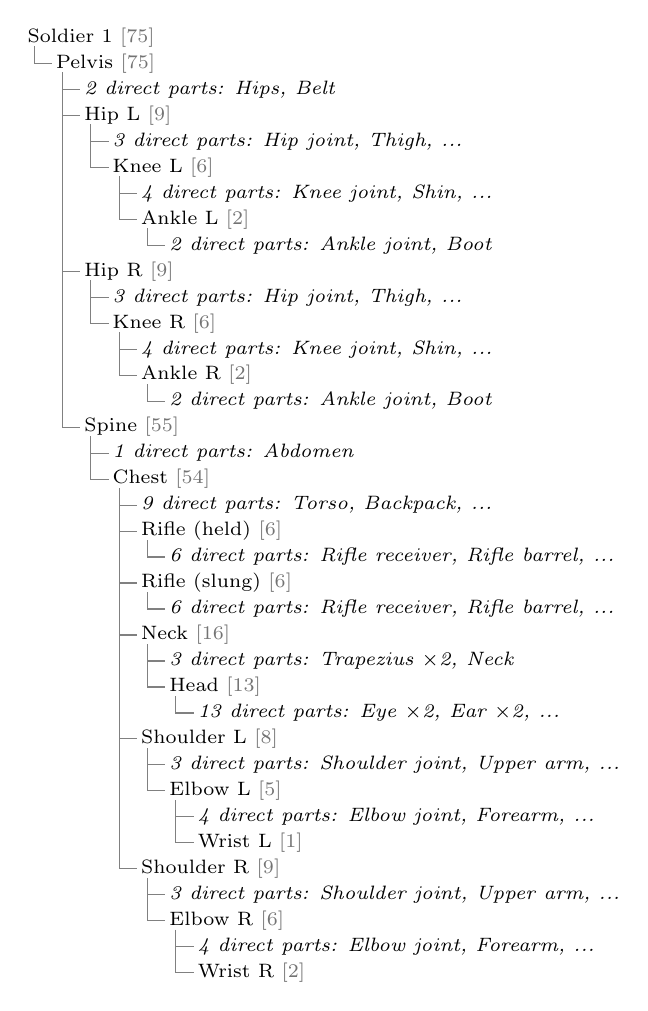
\begin{tikzpicture}[x=0.36cm,y=-0.33cm,font=\scriptsize]
\node[anchor=west,inner sep=0pt] (n0) at (0,0) {Soldier 1 \textcolor{black!55}{[75]}};
\node[anchor=west,inner sep=0pt] (n1) at (1,1) {Pelvis \textcolor{black!55}{[75]}};
\draw[black!50,thin] (0.25,0.35) |- (0.88,1);
\node[anchor=west,inner sep=0pt] (n2) at (2,2) {\textit{2 direct parts: Hips, Belt}};
\draw[black!50,thin] (1.25,1.35) |- (1.88,2);
\node[anchor=west,inner sep=0pt] (n3) at (2,3) {Hip L \textcolor{black!55}{[9]}};
\draw[black!50,thin] (1.25,1.35) |- (1.88,3);
\node[anchor=west,inner sep=0pt] (n4) at (3,4) {\textit{3 direct parts: Hip joint, Thigh, ...}};
\draw[black!50,thin] (2.25,3.35) |- (2.88,4);
\node[anchor=west,inner sep=0pt] (n5) at (3,5) {Knee L \textcolor{black!55}{[6]}};
\draw[black!50,thin] (2.25,3.35) |- (2.88,5);
\node[anchor=west,inner sep=0pt] (n6) at (4,6) {\textit{4 direct parts: Knee joint, Shin, ...}};
\draw[black!50,thin] (3.25,5.35) |- (3.88,6);
\node[anchor=west,inner sep=0pt] (n7) at (4,7) {Ankle L \textcolor{black!55}{[2]}};
\draw[black!50,thin] (3.25,5.35) |- (3.88,7);
\node[anchor=west,inner sep=0pt] (n8) at (5,8) {\textit{2 direct parts: Ankle joint, Boot}};
\draw[black!50,thin] (4.25,7.35) |- (4.88,8);
\node[anchor=west,inner sep=0pt] (n9) at (2,9) {Hip R \textcolor{black!55}{[9]}};
\draw[black!50,thin] (1.25,1.35) |- (1.88,9);
\node[anchor=west,inner sep=0pt] (n10) at (3,10) {\textit{3 direct parts: Hip joint, Thigh, ...}};
\draw[black!50,thin] (2.25,9.35) |- (2.88,10);
\node[anchor=west,inner sep=0pt] (n11) at (3,11) {Knee R \textcolor{black!55}{[6]}};
\draw[black!50,thin] (2.25,9.35) |- (2.88,11);
\node[anchor=west,inner sep=0pt] (n12) at (4,12) {\textit{4 direct parts: Knee joint, Shin, ...}};
\draw[black!50,thin] (3.25,11.35) |- (3.88,12);
\node[anchor=west,inner sep=0pt] (n13) at (4,13) {Ankle R \textcolor{black!55}{[2]}};
\draw[black!50,thin] (3.25,11.35) |- (3.88,13);
\node[anchor=west,inner sep=0pt] (n14) at (5,14) {\textit{2 direct parts: Ankle joint, Boot}};
\draw[black!50,thin] (4.25,13.35) |- (4.88,14);
\node[anchor=west,inner sep=0pt] (n15) at (2,15) {Spine \textcolor{black!55}{[55]}};
\draw[black!50,thin] (1.25,1.35) |- (1.88,15);
\node[anchor=west,inner sep=0pt] (n16) at (3,16) {\textit{1 direct parts: Abdomen}};
\draw[black!50,thin] (2.25,15.35) |- (2.88,16);
\node[anchor=west,inner sep=0pt] (n17) at (3,17) {Chest \textcolor{black!55}{[54]}};
\draw[black!50,thin] (2.25,15.35) |- (2.88,17);
\node[anchor=west,inner sep=0pt] (n18) at (4,18) {\textit{9 direct parts: Torso, Backpack, ...}};
\draw[black!50,thin] (3.25,17.35) |- (3.88,18);
\node[anchor=west,inner sep=0pt] (n19) at (4,19) {Rifle (held) \textcolor{black!55}{[6]}};
\draw[black!50,thin] (3.25,17.35) |- (3.88,19);
\node[anchor=west,inner sep=0pt] (n20) at (5,20) {\textit{6 direct parts: Rifle receiver, Rifle barrel, ...}};
\draw[black!50,thin] (4.25,19.35) |- (4.88,20);
\node[anchor=west,inner sep=0pt] (n21) at (4,21) {Rifle (slung) \textcolor{black!55}{[6]}};
\draw[black!50,thin] (3.25,17.35) |- (3.88,21);
\node[anchor=west,inner sep=0pt] (n22) at (5,22) {\textit{6 direct parts: Rifle receiver, Rifle barrel, ...}};
\draw[black!50,thin] (4.25,21.35) |- (4.88,22);
\node[anchor=west,inner sep=0pt] (n23) at (4,23) {Neck \textcolor{black!55}{[16]}};
\draw[black!50,thin] (3.25,17.35) |- (3.88,23);
\node[anchor=west,inner sep=0pt] (n24) at (5,24) {\textit{3 direct parts: Trapezius $\times$2, Neck}};
\draw[black!50,thin] (4.25,23.35) |- (4.88,24);
\node[anchor=west,inner sep=0pt] (n25) at (5,25) {Head \textcolor{black!55}{[13]}};
\draw[black!50,thin] (4.25,23.35) |- (4.88,25);
\node[anchor=west,inner sep=0pt] (n26) at (6,26) {\textit{13 direct parts: Eye $\times$2, Ear $\times$2, ...}};
\draw[black!50,thin] (5.25,25.35) |- (5.88,26);
\node[anchor=west,inner sep=0pt] (n27) at (4,27) {Shoulder L \textcolor{black!55}{[8]}};
\draw[black!50,thin] (3.25,17.35) |- (3.88,27);
\node[anchor=west,inner sep=0pt] (n28) at (5,28) {\textit{3 direct parts: Shoulder joint, Upper arm, ...}};
\draw[black!50,thin] (4.25,27.35) |- (4.88,28);
\node[anchor=west,inner sep=0pt] (n29) at (5,29) {Elbow L \textcolor{black!55}{[5]}};
\draw[black!50,thin] (4.25,27.35) |- (4.88,29);
\node[anchor=west,inner sep=0pt] (n30) at (6,30) {\textit{4 direct parts: Elbow joint, Forearm, ...}};
\draw[black!50,thin] (5.25,29.35) |- (5.88,30);
\node[anchor=west,inner sep=0pt] (n31) at (6,31) {Wrist L \textcolor{black!55}{[1]}};
\draw[black!50,thin] (5.25,29.35) |- (5.88,31);
\node[anchor=west,inner sep=0pt] (n32) at (4,32) {Shoulder R \textcolor{black!55}{[9]}};
\draw[black!50,thin] (3.25,17.35) |- (3.88,32);
\node[anchor=west,inner sep=0pt] (n33) at (5,33) {\textit{3 direct parts: Shoulder joint, Upper arm, ...}};
\draw[black!50,thin] (4.25,32.35) |- (4.88,33);
\node[anchor=west,inner sep=0pt] (n34) at (5,34) {Elbow R \textcolor{black!55}{[6]}};
\draw[black!50,thin] (4.25,32.35) |- (4.88,34);
\node[anchor=west,inner sep=0pt] (n35) at (6,35) {\textit{4 direct parts: Elbow joint, Forearm, ...}};
\draw[black!50,thin] (5.25,34.35) |- (5.88,35);
\node[anchor=west,inner sep=0pt] (n36) at (6,36) {Wrist R \textcolor{black!55}{[2]}};
\draw[black!50,thin] (5.25,34.35) |- (5.88,36);
\end{tikzpicture}
}\end{minipage}\hfill
\begin{minipage}[c]{0.58\linewidth}\centering
\picsix{soldier_closeup}{0.49\linewidth}\hfill\picsix{soldier_axes}{0.49\linewidth}\\[1mm]
\picsix{soldier_exploded}{0.49\linewidth}\hfill\picsix{soldier_possess_tp}{0.49\linewidth}
\end{minipage}
\caption{Left: node tree of soldier 1 (generated from the export; [n] = leaves below). Right: close-up, joint frames (\texttt{H}), primitive colours (\texttt{E}; the soldier roots are not yet in the explode list, so the parts stay assembled) and a possessed soldier in third person.}\label{fig:soldiertree}\label{fig:soldierviews}
\end{figure}

\subsection{Routes: centripetal Catmull--Rom splines}
\autofig{diagrams}{H3_catmull_rom}
A route through control points $P_0..P_n$ must pass through them, have a continuous tangent and no cusps or loops. A Catmull--Rom spline with knots $t_{i+1}=t_i+|P_{i+1}-P_i|^\alpha$ meets the first two for every $\alpha$; Yuksel et al.\ showed that only the \emph{centripetal} choice $\alpha=\tfrac12$ guarantees no cusp or self-intersection inside a segment. Each segment $P_1\to P_2$ is evaluated as a cubic Hermite curve in $u\in[0,1]$ with end tangents
\begin{equation}
\vect m_1=(t_2-t_1)\Bigl(\tfrac{P_1-P_0}{t_1-t_0}-\tfrac{P_2-P_0}{t_2-t_0}+\tfrac{P_2-P_1}{t_2-t_1}\Bigr),\qquad
\vect m_2=(t_2-t_1)\Bigl(\tfrac{P_2-P_1}{t_2-t_1}-\tfrac{P_3-P_1}{t_3-t_1}+\tfrac{P_3-P_2}{t_3-t_2}\Bigr),
\end{equation}
$\vect r(u)=h_{00}P_1+h_{10}\vect m_1+h_{01}P_2+h_{11}\vect m_2$ with the Hermite basis $h_{00}=2u^3-3u^2+1$, $h_{10}=u^3-2u^2+u$, $h_{01}=-2u^3+3u^2$, $h_{11}=u^3-u^2$. This equals the Barry--Goldman pyramid and is $C^1$ in the knot parameter. Open routes get mirrored phantom end points $2P_0-P_1$. The first and second derivatives come from the same basis, so the curvature is analytic:
\begin{equation}\kappa=\frac{|\vect r'\times\vect r''|}{|\vect r'|^3}\qquad\text{(independent of the parameterisation).}\end{equation}
\lstSplineSeg
\paragraph{Arc length.} Walking at a speed needs $\vect r(s)$ with $s$ in metres. Each segment is cut into 64 chords; their cumulative lengths form a monotone table and $s\mapsto t$ is a binary search plus a linear blend inside the chord (Listing~\ref{lst:ArcLen}). T200 checks interpolation, the joint kink, length and curvature errors (\tobs{T200}).
\lstArcLen

\subsection{Speed along a curve}
People slow down in tight turns. The soldier's speed limit is a function of the curvature,
\begin{equation}v_\kappa(s)=\max\bigl(0.25,\ v_\text{max}/(1+1.5\,\kappa(s))\bigr),\end{equation}
taken as a minimum over the next 0.5\,m. Braking is planned ahead: with a deceleration of $2.5$\,m/s$^2$ a speed $v$ can still reach $v_\kappa(s+a)$ after $a$ metres if $v\le\sqrt{v_\kappa(s+a)^2+2\cdot2.5\,a}$, so the target is the minimum of that bound over $a\in[0,2]$\,m, and $\sqrt{2\cdot1.2\,d}+0.15$ before a stop $d$ metres ahead. The speed approaches the target at $+1.6$/$-4$\,m/s$^2$ and is clamped again at the end of the step because $\kappa$ is only piecewise continuous on a $C^1$ curve (T213: \tobs{T213}).
\lstSpeedLaw

\subsection{The site planner: A*, string pulling, spline}
Routes between camp sites are planned, not drawn. \code{SitePlanner} rasterises the camp onto $72\times72$ cells of 1\,m. Every static part that reaches into the body band (0.15--1.8\,m above the ground) contributes its exact oriented plan footprint (the convex hull of the projected unit primitive under its world matrix); fences, the trench and the HESCO ring are added as segments. A cell is free when its centre keeps 0.40\,m from every footprint. Then:
\begin{enumerate}
\item \textbf{A*} on the 8-connected free cells with the octile heuristic $h=\max(\Delta i,\Delta j)+(\sqrt2-1)\min(\Delta i,\Delta j)$, which is the exact distance on an obstacle-free 8-grid and therefore admissible and consistent; diagonal moves may not cut a blocked corner (Listing~\ref{lst:AStar}).
\item \textbf{String pulling}: from each kept point, the farthest later grid point whose straight segment keeps the clearance (sampled every 0.1\,m) is kept; the staircase of grid steps collapses to a few corners (Listing~\ref{lst:StringPull}).
\item \textbf{Spline} through the kept points, validated every 0.1\,m against a body clearance of 0.28\,m. Where a sample fails, the grid points around it are re-inserted; in the limit the spline passes through every cell centre, whose edges are clear by construction.
\end{enumerate}
The bunker is reached by a hand-authored leg (ramp, blast doors, tunnel, rooms) with floor heights from the walk space. For the \nRoutes{} routes of the roster ($\routeTotal$\,m in total) the smallest clearance is \routeMinClear\,m (Table~\ref{tab:routes}; T205: \tobs{T205}).
\begin{figure}[h]
\centering
\begin{subfigure}{0.495\linewidth}\picsix{plan_routes}{\linewidth}\caption{Tactical map (\texttt{M}): soldier splines and rover via chains}\end{subfigure}
\begin{subfigure}{0.495\linewidth}\picsix{day_patrol_spline}{\linewidth}\caption{Spline routes drawn over the camp by day}\end{subfigure}
\caption{Planned routes (captures).}\label{fig:routes}
\end{figure}
\lstAStar
\lstStringPull
\begin{table}[h]
\centering\scriptsize
\caption{Roster routes (generated from \code{v6.garrison.routes}).}\label{tab:routes}
\tabRoutes
\end{table}

\subsection{Gait: forward kinematics driven by a foot trajectory}
\autofig{diagrams}{H4_gait_cycle}
A walk cycle is defined by where the feet must be, not by key frames. Leg 0 touches down at phase 0, leg 1 at 0.5; the stance lasts the duty fraction $\beta$ of the cycle. With the stride $L$ the ankle position relative to the hip is
\begin{equation}
x_\text{stance}(\sigma)=x_f-(x_f-x_b)\,\sigma,\qquad
x_\text{swing}(\sigma)=x_b+(x_f-x_b)\Bigl(\sigma-\frac{\sin2\pi\sigma}{2\pi}\Bigr),\qquad y_\text{swing}\mathrel{+}=\ell\sin\pi\sigma,
\end{equation}
$x_{f,b}=\pm\tfrac12L\beta-r$ ($\sigma$ = fraction of the stance or swing done, $r$ a push-off offset). In stance the ankle moves backwards at exactly the body speed, so it stands still in the world; the swing is a cycloid, whose velocity relative to the body is zero at lift-off and touch-down (no foot skating). The pelvis bobs twice per cycle, the trunk counter-rotates and each arm swings against its leg (T204: \tobs{T204}). Walk and run differ only in parameters (Table~\ref{tab:gait}). The joint angles that place the ankle there come from IK.
\begin{table}[h]
\centering\small
\caption{Gait parameters (generated from \code{v6.garrison.gait}).}\label{tab:gait}
\tabGait
\end{table}
\lstFootPath

\subsection{Two-link inverse kinematics}
\autofig{diagrams}{H5_two_link_ik}
Thigh $L_1=\gaitThigh$\,m and shin $L_2=\gaitShin$\,m form a triangle with the hip--ankle distance $d=|(x,y)|$, clamped to $[\,|L_1-L_2|,\,L_1+L_2]$. The law of cosines gives
\begin{equation}
\theta_k=\pi-\arccos\frac{L_1^2+L_2^2-d^2}{2L_1L_2},\qquad
\theta_h=\operatorname{atan2}(x,-y)+\arccos\frac{L_1^2+d^2-L_2^2}{2L_1d},
\end{equation}
knee bend $\theta_k$ (0 = straight) and thigh angle $\theta_h$ from the vertical, with the knee in front of the hip--ankle line. Forward kinematics, $x=L_1\sin\theta_h+L_2\sin(\theta_h-\theta_k)$, $y=-L_1\cos\theta_h-L_2\cos(\theta_h-\theta_k)$, closes the loop: T203 measures $|FK(IK(\vect p))-\vect p|$ (\tobs{T203}). In the scene the stance foot's world point is \emph{locked} at touch-down and the IK solves for that point every frame, so the foot does not slide on slopes or in turns (T202: \tobs{T202}). The ankle keeps the sole level (ankle $=\theta_k-\theta_h$) and pivots on the toe at push-off.
\lstLegIK

\paragraph{Arms: two-bone IK with a pole vector (v7).} Armed soldiers hold the rifle with both hands. For a shoulder $S$, a hand target $T$ on the rifle grip and a pole direction $\vect p$ (where the elbow should point), the solver in the chest frame takes $\hat{\vect e}=(T-S)/d$, the pole's part perpendicular to it $\hat{\vect p}_\perp$ and the angle $A$ at the shoulder from the law of cosines; the upper arm is $\hat{\vect u}=\hat{\vect e}\cos A+\hat{\vect p}_\perp\sin A$, the elbow $S+\ell_u\hat{\vect u}$, the forearm $\hat{\vect v}$ points from the elbow to $T$ and the elbow bend is $\arccos(\hat{\vect u}\cdot\hat{\vect v})$. The shoulder rotation is the basis $(\vect x,\vect y,\vect z)=(\vect y\times\vect z,\ -\hat{\vect u},\ \text{forearm direction}\perp\hat{\vect u})$, converted to the rig's Euler order $M=R_yR_xR_z$ by $\text{pitch}=\arcsin(-z_y)$, $\text{yaw}=\operatorname{atan2}(z_x,z_z)$, $\text{roll}=\operatorname{atan2}(x_y,y_y)$.
\lstArmIK

\subsection{Roster, shifts and behaviour}
Each soldier has a duty with a day and a night program (Table~\ref{tab:roster}). The day shift runs from \shiftStart{} to \shiftEnd, matching the DayBreak and Dusk crossings of Section~\ref{sec:daycycle}. At dusk the departures are staggered; soldiers going below walk the ramp, wait at closed blast doors, pass the tunnel and sit down in the bunk room or the mess (T207: \tobs{T207}). A soldier's state machine cycles through Idle, Guard, Work, Sit, Walk, Run, Wait, Duck, Crouch and Wave; work loops play at the vehicles (mechanic's wrench at the tank deck and the helicopter, logistics carrying crates; T210). Walkers yield or pass on the side away from each other with a validated lateral offset (T214: \tobs{T214}). In the thermal view a soldier is warm but never engine-hot: face and hands 0.82, torso 0.70, below the 0.90 core of a rover (T209), and each soldier carries a friendly radius of \soldierFriendly\,m for the squad (Section~\ref{sec:realcv}).
\begin{table}[h]
\centering\scriptsize
\caption{Duty roster (generated from \code{v6.garrison.soldiers}).}\label{tab:roster}
\tabRoster
\end{table}
\begin{figure}[h]
\centering
\begin{subfigure}{0.495\linewidth}\picsix{day_mechanic}{\linewidth}\caption{Mechanic at the tank (wrench)}\end{subfigure}
\begin{subfigure}{0.495\linewidth}\picsix{day_logistics}{\linewidth}\caption{Logistics carrying a crate}\end{subfigure}\\[1mm]
\begin{subfigure}{0.495\linewidth}\picsix{dusk_shift_change}{\linewidth}\caption{Dusk: shift-change banner}\end{subfigure}
\begin{subfigure}{0.495\linewidth}\picsix{bunker_offduty}{\linewidth}\caption{Off duty in the bunk room (night)}\end{subfigure}\\[1mm]
\begin{subfigure}{0.495\linewidth}\picsix{soldier_possess_fp}{\linewidth}\caption{Possessed soldier, first person}\end{subfigure}
\caption{Duties over the day (captures, RTX\,4070).}\label{fig:duties}
\end{figure}
\sheetfig{sheet_soldiers}

% =====================================================================
\section{Random Intruder Paths and Seeded Runs}\label{sec:randompaths}
\pipestrip{10}
In v5 every run replayed the same intruders: a legacy first rover, spawns from a fixed stream and one cost field per objective. Version~6 makes each night different but reproducible: the routes are drawn from distributions (\code{Mission::randomRoute}), every random source is a stream derived from one run seed, and the day cycle adds two rules: waves only at night, and a withdrawal at dawn. The rover's planner itself is unchanged: the weighted Dijkstra field of Section~\ref{sec:rover}, now steered by via points and a personality.

\subsection{Ring spawns, via sectors and personalities}
\autofig{diagrams}{H6_spawn_ring}
A spawn bearing $\phi$ is drawn uniformly on $[0,2\pi)$ and rejected while it lies within $\pm\rrNorthGapDeg^\circ$ of the gate road (north), so the accepted bearings stay uniform on the remaining $360-2\cdot\rrNorthGapDeg$ degrees (T219: \tobs{T219}). The radius is uniform in $16.8\pm\rrSpawnJitter$\,m, just inside the fence. The rover then gets one of the five camp assets as objective and, with equal probability, $0$--$\rrMaxVia$ via points: each at bearing $\phi+U(-\rrViaSectorDeg^\circ,\rrViaSectorDeg^\circ)$ and radius $U(\rrViaMinR,\rrViaMaxR)$\,m, rejected if it is not a free planner cell or lies within 3\,m of the spawn or the objective. Vias are visited outermost first, so the chain closes in on the camp from the rover's own side instead of crossing it (T215: \tobs{T215}).

A \emph{personality} changes how the rover moves between vias: the weight of the random noise field in the route cost $U(8,40)$, the weight of cells a UAV can see $U(12,48)$, a speed factor $U(0.8,1.25)$, a probability $U(0,0.5)$ of pausing 1.5--4\,s on entering cover and a noise lattice of 3--7 cells. The Dijkstra cost of a cell becomes
\begin{equation}c=d+w_e\,[\text{visible to a UAV}]+w_n\,n(\text{cell}),\end{equation}
so a cautious rover detours through cover and a bold one drives straight (T216, three routes from one spawn: \tobs{T216}; T217: \tobs{T217}). With probability \rrSwitchProbability{} the rover switches to a different asset after $U(\rrSwitchMinS,\rrSwitchMaxS)$\,s (T218: \tobs{T218}).
\begin{table}[h]
\centering\small
\caption{Random-route constants (generated from \code{v6.random\_routes}).}\label{tab:rrconst}
\tabRandomRoutes
\end{table}
\lstRandomRoute

\subsection{Day rules and the dawn withdrawal}
Waves start only in the NIGHT phase (T220: \tobs{T220}). At the Dawn event the mission ends the current wave (\code{endNight}) and every intruder still alive is given a retreat goal: the free cell on its own bearing near the fence ring ($r=17.5$\,m). A rover that gets there leaves the field with a \emph{Withdraw} event, which scores nothing and costs no integrity; one that cannot reach an exit within 90\,s (\code{kRetreatTimeout}) is withdrawn anyway (T221: \tobs{T221}). By day the searchlight cones, UAV~1's light and the beacon are off (T222). Figure~\ref{fig:dawn} shows the banner of a real withdrawal.
\begin{figure}[h]
\centering
\picsix{dawn_withdraw}{0.7\linewidth}
\caption{Dawn (05:47): the HUD's DAWN and INTRUDER WITHDRAWS banners after a real Withdraw event (capture, seed 1).}\label{fig:dawn}
\end{figure}

\subsection{One seed, independent streams}
A run has one 32-bit seed: \cli{seed N}, or by default the mix of \code{std::random\_device} and the clock, printed at start and shown in the HUD and the trace header. Each subsystem draws from its own stream $k$:
\begin{equation}
z=b\oplus(k\cdot\texttt{0x9E3779B9}),\quad z\leftarrow(z\oplus z\gg16)\cdot\texttt{0x85EBCA6B},\quad z\leftarrow(z\oplus z\gg13)\cdot\texttt{0xC2B2AE35},\quad z\leftarrow z\oplus z\gg16 .
\end{equation}
This is the splitmix32 finaliser: an invertible avalanche mix in which flipping one input bit flips each output bit with probability $\approx\tfrac12$, so neighbouring stream numbers give unrelated seeds. Streams 1--4 seed the mission, combat effects, the UAV patrol and the garrison; 100 and 101 the two sensors (Table~\ref{tab:seeds}). Seed 0 maps to the legacy v5 constants, which keeps every v5 test bit-exact; a seeded patrol differs from it (base radii \patrolRadii\,m, breathing amplitudes \patrolAmps\,m for seed \seedBase; T223: \tobs{T223}).
\begin{table}[h]
\centering\small
\caption{Derived stream seeds for the example base seed (generated from \code{v6.seeds}).}\label{tab:seeds}
\tabSeeds
\end{table}
\lstDeriveSeed
Same seed, same run: two 600\,s traces with seed 42 are byte-identical and seed 43 differs (Section~\ref{sec:v6results}).

% =====================================================================
\section{Real Computer Vision: Sensor Model, Persons and Guarantees}\label{sec:realcv}
\pipestrip{9}
Up to v5 the vision of Section~\ref{sec:vision} read the ideal heat image the renderer produced. A real uncooled microbolometer adds optics blur, per-pixel gain and offset errors, column stripes, temporal noise, dead pixels, pointing jitter and lost frames. Version~6 models all of them (\code{vision/SensorModel}), adds a person class to the blob filter, and removes every scripted shortcut: a rover can now only be killed through pixels. Figure~\ref{fig:sensorchain} is the per-UAV loop in \code{App::step}.
\begin{figure}[h]
\centering
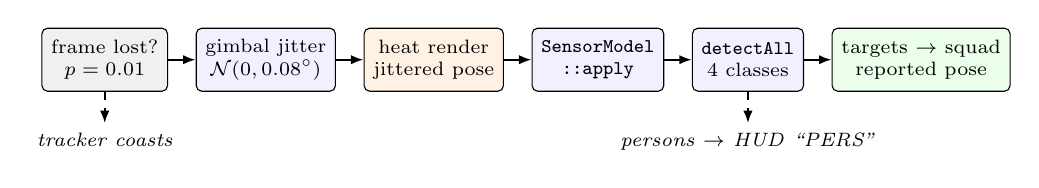
\begin{tikzpicture}[node distance=3mm and 3.5mm, every node/.style={font=\scriptsize},
  box/.style={draw,rounded corners=2pt,minimum height=8mm,align=center,fill=blue!6},arr/.style={-{Latex[length=1.6mm]},thick}]
  \node[box,fill=black!6] (d) {frame lost?\\$p=\snDropProb$};
  \node[box,right=of d] (j) {gimbal jitter\\$\mathcal N(0,\snJitterDeg^\circ)$};
  \node[box,right=of j,fill=orange!10] (r) {heat render\\jittered pose};
  \node[box,right=of r] (s) {\code{SensorModel}\\\code{::apply}};
  \node[box,right=of s] (c) {\code{detectAll}\\4 classes};
  \node[box,right=of c,fill=green!8] (t) {targets $\to$ squad\\reported pose};
  \foreach \x/\y in {d/j,j/r,r/s,s/c,c/t} \draw[arr] (\x)--(\y);
  \node[below=4mm of d,font=\scriptsize\itshape,align=center] (k) {tracker coasts};
  \draw[arr,dashed] (d)--(k);
  \node[below=4mm of c,font=\scriptsize\itshape] (p) {persons $\to$ HUD ``PERS''};
  \draw[arr,dashed] (c)--(p);
\end{tikzpicture}
\caption{One UAV frame in v6. The image is rendered from the jittered gimbal pose, but the detections are reported with the commanded pose, so the pointing error reaches the tracker as measurement noise, as on a real platform.}\label{fig:sensorchain}
\end{figure}

\subsection{The sensor model}
With $x$ the ideal heat image (8-bit digital numbers, DN), the sensor output is
\begin{equation}
y=Q\bigl(g\odot(h*x)+o+c+n\bigr),\qquad n\sim\mathcal N(0,\text{NETD}^2),\qquad
h=\tfrac1{16}\begin{bmatrix}1&2&1\\2&4&2\\1&2&1\end{bmatrix}=\tfrac14[1\ 2\ 1]^\top\,\tfrac14[1\ 2\ 1],
\end{equation}
where $h$ is the optics point-spread function (binomial, applied separably as two 3-tap passes), $g=1+\sigma_g\,\mathcal N$ and $o=\sigma_o\,\mathcal N$ are per-pixel gain and offset, $c$ a per-column offset (readout stripes), $\odot$ the element-wise product and $Q$ rounding to the nearest DN with clamping to $[0,255]$. A fraction $\snStuckFrac$ of the pixels is stuck at 255. $g$, $o$, $c$ and the stuck set are the \emph{fixed pattern}: drawn once per image size from their own random stream, a property of the physical sensor. $n$, the jitter and the drops come from a second, temporal stream (both PCG32 generators; normal deviates by Box--Muller, $z_{0,1}=\sqrt{-2\ln u_1}\,(\cos,\sin)(2\pi u_2)$, the second value kept for the next call). Table~\ref{tab:sensor} lists the defaults.
\begin{table}[h]
\centering\small
\caption{Sensor model and CV thresholds (generated from \code{v6.sensor}).}\label{tab:sensor}
\tabSensor
\end{table}

\paragraph{Non-uniformity correction.} A new sensor is uncalibrated. \code{nuc()} models the two-point shutter calibration of real cameras: the fixed pattern shrinks to $\snNucResidual$ of its raw size, and the stuck pixels seen on the shutter are \emph{mapped out}, each replaced by the mean of its four neighbours (stuck pixels are drawn isolated, so the neighbours are good). Each UAV sensor is seeded from its stream and calibrated once at start. T225 measures the NETD from the difference of two flat frames, in which the fixed pattern cancels (\tobs{T225}); T226 the fixed pattern before and after NUC (\tobs{T226}); T227 the PSF (\tobs{T227}).
\lstSensorApply

\paragraph{Jitter and drops.} Each frame the gimbal is off by $\mathcal N(0,\snJitterDeg^\circ)$ per axis; at $40^\circ$ over 240 rows that is \cvJitterPx\,px. \code{jitterCamera} turns the camera matrix by $R_y R_x$ about its own axes for the render only (T232: \tobs{T232}). With probability $\snDropProb$ a frame is lost; the Kalman tracker predicts through it (confirmed tracks coast, T231: \tobs{T231}). Same seed, same frames: T233 (\tobs{T233}).

\subsection{Four blob classes}
The v5 target filter is kept bit for bit (T236: \tobs{T236}); \code{detectAll} labels every other blob instead of dropping it, from the moments of Section~\ref{sec:vision} (area $A$, peak value, elongation $\varepsilon=\sqrt{\lambda_1/\lambda_2}$, major-axis angle $\theta$):
\begin{center}\small
\begin{tabular}{@{}lp{11.8cm}@{}}\toprule
Class & Rule (in order)\\\midrule
target & $2\le A\le2500$, peak $\ge\snCvCore$ (an engine core) and ($A<6$ or $\varepsilon\le6$)\\
hot clutter & peak $\ge\snCvCore$ but not a target: a fire (too big), a tracer (too thin), a glint\\
person & no hot core; $4\le A\le600$, $\varepsilon\le5$ and upright ($|\theta|\ge45^\circ$ from the image $x$ axis) or compact ($\varepsilon<1.25$, seen from above)\\
clutter & everything else (warm walls, pipes, lying shapes)\\\bottomrule
\end{tabular}
\end{center}
A soldier is warm (face 0.82, $\approx209$\,DN) but has no pixel near the engine level, so he can only become a target if noise lifts a pixel by $\snCvCore-209\approx21$\,DN. Only the target class reaches the squad; persons are drawn as ``PERS'' brackets in the thermal FPV (Figure~\ref{fig:cvnoisecap}). T230: \tobs{T230}; T235 (fire, tracer, pipe): \tobs{T235}.
\lstClassify
\begin{figure}[h]
\centering
\begin{subfigure}{0.49\linewidth}\picsix{lab_cv_noise}{\linewidth}\caption{Ideal vs.\ sensor image, difference, classes}\end{subfigure}
\begin{subfigure}{0.49\linewidth}\picsix{day_thermal_fpv_persons}{\linewidth}\caption{Day thermal FPV: a soldier boxed as PERS}\end{subfigure}
\caption{Real-CV captures. (a) One UAV frame through an ideal and through the modelled sensor, the amplified difference (fixed pattern, stripes, noise) and \code{detectAll}'s classes on the noisy frame. (b) By day the soldiers are the warmest passive shapes; the CV boxes the head and shoulders as a person, not a target.}\label{fig:cvnoisecap}
\end{figure}

\subsection{Detection probability and false alarms against NETD}
\autofig{diagrams}{H7_pd_netd}
The figure-data tool runs the full model on synthetic frames with a rover and a soldier, \cvFrames{} frames per noise level (Table~\ref{tab:pd}). The rover's core reads about 244\,DN after the PSF (T227), 14\,DN above the core threshold; at the default NETD of \snNetdDn\,DN that is 7$\sigma$, and since one core pixel suffices, $P_d=1$ up to NETD \cvNetdWorst. A rover at half size loses more of its small core to the PSF: $P_d$ \cvPdFarNom{} at the default noise, \cvPdFarWorst{} at NETD \cvNetdWorst. False alarms appear only at NETD \cvNetdWorst{} (\cvFalseWorst{} per frame): the 21\,DN margin of a soldier's warmest pixels is then 2.6$\sigma$, $P(z>2.6)\approx0.005$ per pixel, and over the 10--20 pixels of a distant soldier this gives a few per cent, the order of the measured person$\to$target rate. Without NUC at the default noise a stuck pixel on a soldier becomes a ``hot core'': \cvNoNucFalse{} false targets and \cvNoNucPerson{} person-as-target per frame, which is why the sensors are calibrated at start.
\begin{table}[h]
\centering\small
\caption{Detection statistics against NETD (generated from \code{cv\_noise.json}, \cvFrames{} frames per row, after NUC except the last row).}\label{tab:pd}
\tabPd
\end{table}

\subsection{Why a blind squad never fires}
Version~5 had capture-only shortcuts (a scripted strike, forced kills). They are gone; a kill now needs the whole chain. The guarantee rests on four facts that tests or the trace check:
\begin{enumerate}
\item Rounds are launched only from the squad's launch orders, which aim at a \emph{confirmed} track of the shared tracker (Section~\ref{sec:squad}).
\item The tracker is fed only by \code{submitVision}, i.e.\ by Target blobs of a noisy sensor image; with no image there are no tracks: 120\,s of rovers infiltrating in front of a squad without frames (T234: \tobs{T234}).
\item Persons are never targets in the test frames (T229: \tobs{T229}; T230), and a blob whose ground point lies inside a friendly mark is discarded before the tracker: every controllable reports a friendly radius (soldier \soldierFriendly\,m, vehicle 4.5\,m; T224: \tobs{T224}).
\item The 600\,s traces count rounds without a confirmed vision track, kills without a UAV round and spawns by day: all zero (Section~\ref{sec:v6results}).
\end{enumerate}
\sheetfig{sheet_cvnoise}

% =====================================================================
\section{Version 6 Results}\label{sec:v6results}
All v6 numbers below were produced by the program on the RTX\,4070 machine (\runGpu, EPIC preset) or by the CPU test binary; the tables are generated from the trace logs and \code{test\_results.json} by \code{report/gen\_v6.py}.

\paragraph{Unit tests.} \nVsixTests{} v6 tests, \nVsixPass{} pass (Table~\ref{tab:v6tests}); together with v5 and the later v7 work, \nTests{} tests run, \nPass{} pass (Table~\ref{tab:testareas}).
\begin{table}[h]
\centering\small
\caption{v6 tests by work package (generated).}\label{tab:v6tests}
\tabVsixTests
\end{table}

\paragraph{Determinism and game rules (600\,s traces).} \code{-{}-trace FILE 600 -{}-time cycle -{}-seed S} plays two full day--night cycles from 23:00 with the auto clock and writes a 4\,Hz state CSV, an event CSV and a rule check. Seed 42 was run twice: the trace and event files are \runSame{} (MD5 \runMdA{}); seed 43 gives a different game (\runMdC{}). Phase events of both seeds: \runPhaseEvents. Intruders spawned only in the \runSpawnPhases{} phase. Withdrawals for seed 42 at \runWithdrawA{} and for seed 43 at \runWithdrawC: one in the Dawn step itself and one exactly \code{kRetreatTimeout} later, a rover that found no exit cell. Table~\ref{tab:v6runs} lists the game outcome and the rule check.
\begin{table}[h]
\centering\scriptsize\setlength{\tabcolsep}{3.5pt}
\caption{600\,s traces, two cycles each. $^*$Rule violations: spawns by day / kills without a UAV round blast / rounds without a confirmed vision track (computed by \code{traceMode} from the event stream).}\label{tab:v6runs}
\tabRuns
\end{table}
Every kill followed a UAV round on a vision track, so the guarantee of Section~\ref{sec:realcv} holds in play, not only in tests. About 1\,\% of the frames are dropped, as configured. The balance is open: the breaches are as many as the kills.

\paragraph{Night regression against v5.} The v5 shot list was re-captured with \code{-{}-time night -{}-seed 0 -{}-no-garrison} (night preset, legacy seeds, no soldiers) and compared with the v5 figures pixel by pixel (Table~\ref{tab:nightreg}, mean absolute error on 0--255 and PSNR). The \nrStaticN{} static views (no game event in the frame) differ by at most \nrStaticMax{} (PSNR $\ge$ \nrStaticMinPsnr\,dB): smoke and fire positions, nothing structural. The event shots differ because the game differs: v5's frames came from the removed scripted strike, v6's from real kills under sensor noise; the HUD also gained the clock panel. Median over all \nrCount{} shots: \nrMedian. The night preset therefore reproduces the v5 renderer.
\begin{table}[h]
\centering\scriptsize\setlength{\tabcolsep}{4pt}
\caption{Night regression, v6 night preset vs.\ the v5 captures (generated from the two image sets).}\label{tab:nightreg}
\tabNightReg
\end{table}

\paragraph{Captures.} The 18 v6 shots were rendered headless on the RTX\,4070 (EPIC, $1920\times1080$, seed 1; \code{report/figures\_v6}) and each image was reviewed. Most wait for a real game state (a Withdraw event, a mechanic ``WORKING AT MBT-2'', three soldiers seated off duty) rather than a fixed time, so they show the simulation, not a staged pose. They appear in Figures~\ref{fig:sky}, \ref{fig:soldierviews}, \ref{fig:routes}, \ref{fig:duties}, \ref{fig:dawn} and~\ref{fig:cvnoisecap}.

\paragraph{Open issues.} The soldier roots are not in the explode list, so the \texttt{E} view shows them assembled (Figure~\ref{fig:soldierviews}). The day sky's straight cloud seams seen in the first v6 captures came from a float lattice hash and were fixed in v7 by an integer hash; the published day captures predate that fix. A v6 demo video has not been recorded yet (the recorder works: H.264 1080p30 + AAC), and frame times on the RTX are still not measured.

% =====================================================================
\section{Limitations and Conclusion}\label{sec:results}
\subsection{What was measured}
\sheetfig{s00_cover_kpis}
\begin{table}[h]
\centering\small
\caption{Quantities taken from the program output of this report's build (not from memory).}
\label{tab:measure}
\begin{tabular}{@{}p{8.7cm}p{7.2cm}@{}}
\toprule
Quantity & Value (source)\\\midrule
Leaf parts in the scene, in \nObjects{} export objects & \nLeaves{} (\code{scene\_export.json}, Table~\ref{tab:parts})\\
Parts with emissive $>0$ & \nEmissive{} (\code{scene\_export.json})\\
Track links of the tank & \nTrackLinks{} (export; T80)\\
Mesh memory, indexed vs non-indexed & \memIndexed{} B vs \memNonIndexed{} B (Table~\ref{tab:memory})\\
Automated tests & \nTests{} run, \nPass{} pass, \nFail{} fail (\code{test\_results.json})\\
Terrain & 49\,921 vertices, 97\,440 triangles, 36\,m radius (T13, T61)\\
Bunker clear height / walk eye height & 2.60\,m / 1.7\,m (T62, T51)\\
Missile: first launch request after lock & 1.53\,s (T108); detonation 0.50\,m from the spot (T100)\\
Shell range on level ground & 203.8\,m, $-0.24$\,\% from theory (T101)\\
Debris: pieces at rest within 8\,s & 23 of 23 (T106)\\
180\,s headless run: UAV max radius, min clearance, rover hidden & 15.57\,m, 5.62\,m, 61\,\% of frames (T45)\\
Full base, 120\,s simulated & 9 controllables (7 possessable), finite state (T113)\\
\textbf{FPS / ms per frame on the RTX 4070} & \sNM; command in Section~\ref{sec:platform}\\\bottomrule
\end{tabular}
\end{table}

Up to v5 no frame time was measured, and the EPIC preset was exercised only on llvmpipe; the v6 and v7 runs on the RTX 4070 are covered in Section~\ref{sec:v6results}. The GPU timer labels in Section~\ref{sec:pipeline} are what \cli{benchmark} reports on the RTX machine.

\subsection{Limitations}
\begin{itemize}
  \item \textbf{Verification environment.} Up to v5, every capture and test run used Mesa llvmpipe, and the visual tuning (explosion brightness, interior exposure) was done on llvmpipe images. From v6 on, captures and tests run on the RTX 4070 through the WSL2 D3D12 driver; Section~\ref{sec:v6results} gives those results.
  \item \textbf{Windows.} The executable is cross-compiled with zig and has never been run natively.
  \item \textbf{Soft particles.} The effect shader supports a soft depth fade but the renderer passes \code{uHasSceneDepth=0}, so smoke clips hard against geometry.
  \item \textbf{Combat scope.} Hit tests use spheres (rovers, radius 0.4\,m) and boxes (static solids), not part meshes. The player's machines have no damage state other than camouflage scorching, and nothing can hit a UAV.
  \item \textbf{Exporter.} It labels surfaces 12--18 as ``Other'' and the terrain mesh function string with radius 20 (stale labels).
\end{itemize}

\subsection{Conclusion}
ThermalSense is a night military base built within the lab's rules: \nLeaves{} parts, all unit cubes, spheres, cylinders and cones with $T\,R\,S$ transforms,
share six indexed meshes. It has a walkable underground bunker with eased blast doors, a base apron with an animated flag, windsock and gate, and machines with
non-trivial motion (arc-length track links, skid steer with a stabilised turret, a cyclic rotor with a spring-damper attitude, a spooling Gatling gun, three radar modes). Two UAVs render the scene as heat, a computer-vision
pipeline and a multi-target tracker turn it into tracks, and a squad coordinates proportional-navigation strikes on armoured, infiltrating rovers (Chapters~\ref{sec:vision}, \ref{sec:squad}); the game logic is deterministic and covered by \nTests{} CPU tests, \nPass{} of which pass.
The remaining work is measurement, not construction: FPS on the RTX 4070 and a native Windows run. The audit in Appendix~\ref{app:audit} lists every item and its evidence.


\appendix
\section{Audit}\label{app:audit}
Each requirement with a status, evidence and remark. \sDone{} = implemented and verified by a test, a measurement or a code reading; \sPart{} = implemented but not fully verified or with a known gap;
\sNM{} = not measured (hardware not available). Evidence is \code{file:line} (lines may drift), a test id (T..; Table~\ref{tab:alltests}) or a figure.

{\scriptsize\setlength{\tabcolsep}{2.5pt}
\renewcommand{\arraystretch}{1.05}
\begin{longtable}{@{}p{0.4cm}p{4.3cm}p{1.15cm}p{4.9cm}p{5.5cm}@{}}
\toprule \# & Item & Status & Evidence & Remarks\\\midrule\endfirsthead
\toprule \# & Item & Status & Evidence & Remarks\\\midrule\endhead
\bottomrule\endfoot
\multicolumn{5}{@{}l}{\textbf{A. Lab sheet and proposal (R01--R26 of docs/PLAN.md)}}\\
A1 & Unit cube / sphere / cylinder centred at origin & \sDone & \code{src/primitives/*}; T01--T09 & ext.\ $\pm0.5$ verified\\
A2 & Unique vertices + index buffer; saving & \sDone & \code{MeshData}; T12; Table~\ref{tab:memory} & 66.6\,\% sphere, 66.5\,\% terrain\\
A3 & VAO/VBO/EBO, stride 24\,B & \sDone & \code{rendering/Mesh.cpp}; \S\ref{sec:prims} & not run on a GPU\\
A4 & CCW front faces + culling & \sDone & T03, T09, T10, T11 & \\
A5 & 36 slices, sphere by reflection, cylinder on $z$ & \sDone & T04--T08 & \\
A6 & $M=T\cdot R\cdot S$, $W=$ parent$\cdot$local & \sDone & T14, T15; \S\ref{sec:transform} & workbook check: max $|M-M_\text{code}|=2.4\times10^{-5}$\\
A7 & Flat bunker / Gouraud terrain / Phong UAV & \sDone & T19 & per-object shading assignment\\
A8 & Three lights (moon, beacon, searchlight) & \sDone & \code{Lighting.h}; \code{Scene.cpp:updateLightsAndBeam} & keys 1--3\\
A9 & Z-buffer; depth test off (\texttt{Z}) & \sDone & Fig.~\ref{fig:diag}; \code{Interactive.cpp} key Z & \\
A10 & Hidden-line / x-ray edges (\texttt{X}) & \sDone & \code{Interactive.cpp} key X & \\
A11 & Hierarchical searchlight & \sDone & T21 & \\
A12 & Thermal colour map, 4 palettes & \sDone & \code{ThermalPalette.h} & \\
A13 & Only primitives, no models / textures & \sDone & T38, T70, T67, T96, T99 & procedural shader patterns only\\
A14 & Excel workbook from program output & \sDone & \code{tools/build\_workbook.py}, \code{verify\_workbook.py} & verify PASS; crops in this report\\
A15 & Real measurements only; FPS on RTX 4070 & \sNM & \S\ref{sec:platform} & \code{-{}-benchmark} command given\\
\midrule
\multicolumn{5}{@{}l}{\textbf{B. Objects (part counts from the export)}}\\
B1 & Underground bunker (\partsBunker{} parts) & \sDone & \code{objects/Bunker.cpp}; T60--T69 & rooms: \S\ref{sec:walk}\\
B2 & Blast doors & \sDone & \code{Bunker.cpp:28}; T64, T65 & starts open\\
B3 & Base apron (\partsBase{} static) & \sDone & \code{objects/Base.cpp}; T70--T79 & \\
B4 & HESCO wall (204 cells), 4 towers, gate, helipad, motor pool, depot, barracks & \sDone & T72, T71, T77 & \\
B5 & UAV with launcher rails (\partsUav{}) & \sDone & \code{objects/Uav.cpp:100}; T112 & 4 rounds\\
B6 & Intruder rover (\partsRover{} each, up to 6) & \sDone & \code{objects/Rover.cpp}; \code{kMaxRovers} & \\
B7 & Tank (\partsTank{}, 80 links) & \sDone & \code{objects/Tank.cpp}; T80--T87 & \\
B8 & AA Gatling gun (\partsAa{}, 6 barrels) & \sDone & \code{objects/AaGun.cpp}; T88, T89 & \\
B9 & Helicopter (\partsHeli{}, 5 blades) & \sDone & \code{objects/Helicopter.cpp}; T90--T96 & \\
B10 & Radar (\partsRadar{}, 21 tiles) & \sDone & \code{objects/Radar.cpp}; T97--T99 & \\
B11 & Gate barrier (\partsBarrier{}) & \sDone & \code{Base.cpp:682}; T73 & \\
B12 & Windsock (\partsWindsock{}, 5 segments), flag (\partsFlag{}, 12 strips) & \sDone & \code{Base.cpp:743, 804}; T74, T75 & scenery, not possessable\\
B13 & Environment (\partsEnv{}), backdrop (\partsBackdrop{}), terrain 36\,m & \sDone & T13, T38--T43, T60, T78, T79 & \\
B15 & Hierarchy diagrams and $M$ examples & \sDone & Figs.\ \ref{fig:tree-bunker}--\ref{fig:tree-air}; Table~\ref{tab:mexamples} & generated from export\\
B16 & Exploded view & \sPart & \code{updateNode()} & bunker, UAV, rover only\\
\midrule
\multicolumn{5}{@{}l}{\textbf{C. Controllable objects and key bindings}}\\
C1 & Keys 5/6/7/8/9/0 possess tank/heli/AA/radar/doors/UAV & \sDone & \code{Interactive.cpp:173--178}; \code{Control.cpp:9}; T127 & \\
C2 & \texttt{[ ]} cycle, \texttt{Backspace} release & \sDone & \code{Interactive.cpp:179--181}; T128 & 9 possessable\\
C3 & \texttt{Enter}/\texttt{Ctrl} fire, door toggle in walk mode & \sDone & \code{Interactive.cpp:183}; T128 & 3.5\,m\\
C4 & \texttt{\textbackslash} action & \sDone & \code{Interactive.cpp:182} & heli, radar, UAV assist, doors\\
C5 & \texttt{C} camera cycle; sight toggle & \sDone & \code{Interactive.cpp:153}; T55 & \\
C6 & \texttt{K} director (13 shots, 120\,s) & \sDone & \code{Director.cpp}; T125, T129 & \\
C7 & \texttt{V Y T Q X Z O F G P} & \sDone & \code{Interactive.cpp:189--212} & view, thermal, edges, shading\\
C8 & \texttt{1 2 3 4}, \texttt{B N}, \texttt{E H M I} & \sDone & \code{Interactive.cpp:198--205} & \\
C9 & \texttt{F5--F10, L J R, +/-, U, Tab, Space, F1, F12, Esc} & \sDone & \code{Interactive.cpp:207--226} & read from code, not pressed on a display\\
C10 & Tank motion: arc-length links, skid steer, stabilised turret & \sDone & \code{Tank.cpp:72, 479}; T80--T86 & \\
C11 & Helicopter state machine, cyclic, spring attitude & \sDone & \code{Helicopter.cpp:409, 453}; T90--T95 & \\
C12 & Gatling spin-up / 30 rps tracers & \sDone & \code{AaGun.cpp:168}; T88 & \\
C13 & Radar modes ROTATE / SECTOR / STOP & \sDone & T97--T99 & \\
C14 & Door easing, barrier easing & \sDone & \code{Bunker.cpp:28}, \code{Base.cpp:682}; T65, T73 & \\
C15 & Flag travelling wave, windsock chain & \sDone & T74, T75 & \\
C16 & UAV manual flight + gimbal assist & \sDone & \code{Scene.cpp:96} & no dedicated test beyond T113 (\sPart)\\
C17 & Interactive input on a real display & \sNM & --- & keys read from code; GLFW path not exercised\\
\midrule
\multicolumn{5}{@{}l}{\textbf{D. Game logic}}\\
D1 & Intruder life cycle & \sDone & \code{Scene.cpp}; T107 & \\
D2 & Locks: lead 0.8\,s, wing 0.5\,s, solo 1.3\,s & \sDone & \code{Squad.h}; T108, T141 & \\
D3 & Laser spot, 4 rails, 6\,s reload & \sDone & \code{Scene.cpp:388}; T112 & \\
D4 & Friend or foe, keep-out, wreck discrimination & \sDone & \code{DroneController.cpp:123, 166}; T109--T111 & \\
D5 & PN homing, ballistic shell, tracer segment tests & \sDone & \code{Combat.cpp:296, 315}; T100--T102 & \\
D6 & Blast damage, explosion effects, cap & \sDone & \code{Combat.cpp:164}; T103--T105 & \\
D7 & Rigid-body debris, burning wreck, respawn & \sDone & \code{Scene.cpp:418, 462, 490}; T106, T107 & \\
D8 & Hiding planner (flood fill + LFR) & \sDone & \code{HideController.cpp}; T26--T28, T44 & \\
D9 & Behaviour statistics (90\,s game trace) & \sDone & \code{docs/v5\_notes/runs/trace\_v5\_low\_90s.csv} & 21 rounds, 12 hits, 3 kills\\
\midrule
\multicolumn{5}{@{}l}{\textbf{E. Render passes (GPU timer labels) and shaders}}\\
E1 & uav camera (CV) raw heat & \sPart & \code{Renderer.cpp} & seen only via llvmpipe\\
E2 & shadow maps: moon $\times2$, static cache, spot & \sDone & \code{RendererFrame.cpp:124}; T33--T35 & \\
E3 & pre-pass, SSAO & \sPart & \code{RendererFrame.cpp} & llvmpipe images only\\
E4 & volumetric fog + shaft & \sPart & \code{ShadersPost.cpp:228} & ditto\\
E5 & scene: sky, parts, grass, foliage, rain, effects & \sPart & \code{Renderer.cpp:468} & ditto\\
E6 & combine + SSR, TAA, exposure / AGC & \sPart & \code{ShadersPostFx.cpp} & ditto\\
E7 & lens flare, DOF, bloom, composite (ACES / FLIR) & \sPart & \code{ShadersPostFx.cpp} & ditto\\
E8 & Surfaces 12--18 & \sDone & \code{ShaderSources.cpp:340--383}; Table~\ref{tab:surfaces} & exporter shows ``Other''\\
E9 & 16 practical lights + dynamic lights & \sDone & \code{Renderer.h:207}; \code{RendererFrame.cpp:268} & no unit test (GPU)\\
E10 & Indoor mask & \sDone & \code{ShaderSources.cpp:79, 177} & T69 (volumes)\\
E11 & Effects renderer, 8 particle types, soft particles & \sDone & \code{Effects.h}, \code{RendererFrame.cpp} & pre-pass depth fade\\
E12 & GLSL compile on an NVIDIA driver & \sNM & --- & only Mesa\\
\midrule
\multicolumn{5}{@{}l}{\textbf{F. Builds and targets}}\\
F1 & Linux headless \code{make HEADLESS=1} & \sDone & this report's test build & \\
F2 & Test binary, JSON output & \sDone & \nTests{} tests, \nFail{} fail & \\
F3 & Exporter / \code{make docs} & \sDone & \code{build/scene\_export.json} & \\
F4 & Linux GLFW, CMake & \sPart & \code{Makefile}, \code{CMakeLists.txt} & not re-run\\
F5 & Windows exe (zig cross-link) & \sPart & \code{tools/cross\_build\_windows.sh} & never run natively\\
F6 & Windows MinGW \code{build.bat}/\code{run.bat} & \sNM & --- & \\
F7 & RTX 4070 run, FPS, NVENC & \sPart & \S\ref{sec:platform}, \S\ref{sec:v6results} & v6 captures and traces on the RTX (d3d12, EPIC); FPS and NVENC not measured\\
F8 & 120\,s demo video & \sDone & \code{report/demo\_v5.mp4} & 1280$\times$720, 30\,fps, AAC audio\\
\midrule
\multicolumn{5}{@{}l}{\textbf{H. Squad, mission, camp and course checklist}}\\
H1 & Waves of rovers that keep spawning, random paths, MicroMouse + line follower & \sDone & \code{Mission.cpp}; \code{HideController.cpp:222}; T143, T144, T180 & weighted Dijkstra + noise\\
H2 & Two UAVs patrol constantly & \sDone & \code{ai/Squad.cpp}; T139 & opposite phase, 21.6\,m apart\\
H3 & Coordinated tracking with computer vision & \sDone & \code{vision/CvPipeline.cpp}, \code{MultiTracker.cpp}; T130--T137, T142 & Kalman, Hungarian, triangulation\\
H4 & Combined attack, two rounds, time-on-target & \sDone & \code{Squad.cpp:43}; T138, T141 & flight-time error 0.7\,\%; blast pair 0.00\,s apart\\
H5 & Hits marked like a game (markers, score, banners) & \sDone & \code{HudMath.cpp}, \code{AppHud.cpp}; T170--T178 & HUD seen only on llvmpipe captures\\
H6 & Sound & \sDone & \code{src/audio}; T160--T169 & RMS $-22$\,dBFS; not tuned by ear\\
H7 & Pro reflection / colour / shading & \sPart & \code{ShaderSources.cpp} & bump + SSR done; no reflection probe\\
H8 & Hidden army camp, launchers, tanks & \sDone & \code{Launchers.cpp}, \code{Base.cpp}; T150--T159 & lights 21 $\to$ 11; SAM, MLRS, 2 parked tanks\\
H9 & Rule ``4--5 shots = 1 kill'' & \sDone & \code{Scene.h:62--63}, \code{Scene.cpp:501}; T105, T140 & 100 HP, 30 $\times$ power $\times$ falloff\\
H10 & Base integrity, base lost, score & \sDone & \code{Mission.cpp}; T181 & \\
H11 & Headless real-render run (LOW, 90\,s) & \sDone & \code{docs/v5\_notes/runs/} & 21 rounds, 12 hits, 3 kills\\
H12 & v5 captures in \code{report/figures\_v5} & \sDone & Figs.\ \ref{fig:v5game}, \ref{fig:v5camp}, \ref{fig:strike} & \\
H13 & Course: 10-slide deck, outline on slide 2 & \sDone & \code{report/ThermalSense\_Presentation.pptx} & \code{tools/build\_slides.py}\\
H13b & Course: 2-minute video at the end of the slides & \sDone & slide 10 & \code{demo\_v5.mp4} embedded\\
H14 & Course: dynamic and controllable objects, complex motion & \sDone & \S\ref{sec:control}; SAM and MLRS slews & 7 + SAM + MLRS\\
H15 & Course: report with audit & \sDone & this document & \\
\midrule
\multicolumn{5}{@{}l}{\textbf{I. Version 6: day cycle, soldiers, random routes, real CV}}\\
I1 & Solar position, phases with hysteresis, phase events & \sDone & \code{DayCycle.cpp}; T190, T194, T199 & sunrise \dcSunrise, sunset \dcSunset, noon $\dcNoonElev^\circ$; Excel recomputes $e$ (sheet 21)\\
I2 & Night preset = v5; day preset; log-space blend & \sDone & T192, T193; Table~\ref{tab:nightreg} & static v5 shots MAE $\le$ \nrStaticMax\\
I3 & Kasten--Young sun colour, quantised key direction & \sDone & T193, T195; Fig.~\ref{fig:diagrams:H2_kasten_young} & \\
I4 & Clouds and cloud shadows (shared CPU / GLSL field) & \sDone & T198; Fig.~\ref{fig:sky} & seams fixed in v7; day captures predate the fix\\
I5 & Solar loading below the CV floor & \sDone & T196 & passive surfaces $\le0.75<0.80$\\
I6 & SKY clock controllable (sun sphere) & \sDone & T197 & \\
I7 & Soldier figure from primitives (\soldierParts{} leaves, depth \soldierDepth) & \sPart & T201; Fig.~\ref{fig:soldiertree} & explode view (\texttt{E}) skips the soldier roots\\
I8 & Centripetal Catmull--Rom, arc length, curvature speed law & \sDone & \code{Spline.cpp}; T200, T213 & \\
I9 & Site planner A* $\to$ string pulling $\to$ spline, clearance & \sDone & \code{Garrison.cpp}; T205 & min clearance \routeMinClear\,m over \nRoutes{} routes\\
I10 & Gait by FK + two-link leg IK, planted feet & \sDone & \code{Gait.cpp}; T202--T204 & \\
I11 & Arm IK rifle hold (v7) & \sPart & \code{Gait.cpp:armIK} & no dedicated test; checked on captures\\
I12 & Roster, shifts, bunker legs, work loops, separation & \sDone & T206, T207, T210, T214 & \\
I13 & Soldier possession, blast duck, heat & \sDone & T208, T209, T211, T212 & no damage model by design\\
I14 & Random routes: ring, vias, personality, switch & \sDone & \code{Mission.cpp}; T215--T219 & \\
I15 & Waves only at night, dawn withdrawal, day lights & \sDone & T220--T222; Table~\ref{tab:v6runs} & 0 spawns by day in 1200\,s of traces\\
I16 & One run seed, derived streams, reproducibility & \sDone & T223, T233; Table~\ref{tab:v6runs} & seed 42 twice: identical traces\\
I17 & Sensor model (PSF, FPN, NUC, NETD, stuck, jitter, drops) & \sDone & \code{SensorModel.cpp}; T225--T228, T231, T232 & \\
I18 & Person class; persons never targets & \sDone & T229, T230, T235, T236 & person$\to$target 0 up to NETD 4\\
I19 & Kills only through vision (no scripted strikes) & \sDone & T234; traces' rule check & 0 violations\\
I20 & CLI, keys, HUD clock and banners, v6 director cut & \sDone & T237--T239; Table~\ref{tab:keysv6} & \\
I21 & v6 captures on the RTX\,4070 (18) & \sDone & \code{report/figures\_v6} & all reviewed\\
I22 & v6 demo video & \sPart & --- & recorder verified; v6 cut not recorded yet\\
\midrule
\multicolumn{5}{@{}l}{\textbf{G. Known issues}}\\
G1 & Verification on llvmpipe only (v2--v5) & \sPart & \S\ref{sec:v6results} & v6 visuals checked on the RTX\,4070; v5 figures still llvmpipe\\
\end{longtable}}



\section{Controls}\label{app:controls}
The key map follows the program's help screen (F1). The possession cycle \texttt{[ ]} also visits the SAM and MLRS launchers (\texttt{\textbackslash} stows or readies, arrows aim, \texttt{Enter} fires).

\begin{table}[h]
\centering\small
\caption{Key bindings (verified in \code{Interactive.cpp}, \code{Control.cpp}; F1 shows the same list in the program).}
\label{tab:keys}
\begin{tabular}{@{}p{3.6cm}p{12.4cm}@{}}
\toprule
Key & Action\\\midrule
\texttt{5} \texttt{6} \texttt{7} & possess the tank / the helicopter / the AA gun\\
\texttt{8} \texttt{9} \texttt{0} & possess the radar / the blast doors / the UAV (manual flight)\\
\texttt{[} \texttt{]} & cycle through the possessable objects (the flag and windsock are skipped; \nPossessable{} possessable, including the soldiers and the SKY clock)\\
\texttt{Backspace} & release the possessed object (the UAV flies itself again)\\
\texttt{W A S D} & drive / fly / turn (in walk mode: walk, \texttt{Shift} runs; free camera: move)\\
\texttt{PgUp PgDn} & climb and descend (helicopter, UAV); free camera\\
\texttt{Arrows}, mouse & aim: turret and gun, AA gun, gimbal, searchlight, radar (arrows held; mouse look as a delta)\\
\texttt{Enter} / \texttt{L-Ctrl} & fire (tank shot, AA burst while held, UAV missile) or toggle (doors, barrier, searchlight, radar TX)\\
\texttt{\textbackslash} & secondary action: start / land (helicopter), radar mode, gimbal assist (UAV), doors / barrier\\
\texttt{Shift} & boost (tank $\times1.5$, helicopter 25\,m/s, UAV 9\,m/s)\\
\texttt{C} & camera cycle: Orbit, Free, Chase, UAV CAM, Walk (T55); while possessing: switch chase view $\leftrightarrow$ sight\\
\texttt{K} & cinematic director (restarts the world; v6 cut: 15 shots in 120\,s, night battle, dawn time-lapse, day duties, dusk, searchlights, the clock forced per shot); again to leave\\
\texttt{V} / \texttt{Y} / \texttt{T} / \texttt{Q} & view: thermal, visible, diagnostic, depth; first-person or external thermal; palette; force a NUC\\
\texttt{X} \texttt{Z} & edges (solid, hidden-line, x-ray); depth test on/off\\
\texttt{O} \texttt{F} \texttt{G} \texttt{P} & shading: per object, all Flat, all Gouraud, all Phong\\
\texttt{1} \texttt{2} \texttt{3} \texttt{4} & toggle moon, beacon, searchlight, practical lights\\
\texttt{B} \texttt{N} & PBR vs Blinn--Phong; full pipeline vs the v1 look\\
\texttt{E} \texttt{H} \texttt{M} \texttt{I} & explode view; local axes; MicroMouse flood field and line guide; indexed or flat drawing\\
\texttt{F5}--\texttt{F10} & quality preset; TAA; SSR; lens flare; auto-exposure; depth of field\\
\texttt{L} \texttt{J} \texttt{R} & foliage cards; fireflies; rain\\
\texttt{+} \texttt{-} & exposure\\
\texttt{U} \texttt{Tab} \texttt{Space} \texttt{F1} \texttt{F12} \texttt{Esc} & UAV feed; HUD; pause; help; screenshot; quit\\\bottomrule
\end{tabular}
\end{table}

\begin{table}[h]
\centering\small
\caption{Keys added in v6 (generated from \code{v6.keys}, the same table as \code{HudMath::keyBindingsV6()} and the F1 overlay). Command line: \cli{seed N}, \cli{time day|night|dusk|dawn|cycle|HH:MM}, \cli{cycle-seconds N}, \cli{no-garrison}.}
\label{tab:keysv6}
\tabVsixKeys
\end{table}



\end{document}
